%! Author = Matthew Magin
%! Date = 17.06.2023

% Preamble
\documentclass[dvipsnames, 11pt]{article}
\usepackage{stmaryrd}

% Packages


%вставка изображений и картинок всяких

\usepackage{graphicx}
\newcommand{\incfig}[1]{%
    \def\svgscale{1.5}
    \import{./figures/}{#1.pdf_tex}
}
\graphicspath{{pictures/}}
\DeclareGraphicsExtensions{.pdf,.png,.jpg, .jpeg, .tex}

\usepackage{booktabs} % для таблиц
\usepackage{enumitem} % для списков


% Шрифты

\usepackage[english,russian]{babel}
\usepackage[T1]{fontenc}
\usepackage{libertine}


\usepackage{titling} % для \maketitle
\usepackage{textcomp}% специальные символы в тексте

\usepackage{mathtext}
\usepackage{amsmath,amsfonts,amssymb,amsthm,mathtools} % математика
\usepackage{icomma} % умная запятая
\usepackage{import} %  импортирование


\usepackage{pdfpages} % мультри-пдф страницы
\usepackage{transparent} % что-то про цвета


\usepackage{caption} % комментарии к figure
\usepackage{epigraph} % эпиграфы

\usepackage{comment} % удобные комментарии
\usepackage{xfrac} % дроби
\usepackage{moresize} % все размеры шрифтов
\usepackage{dsfont} % mathbb для всего


% Окружения для математики:

\newtheorem{statement}{Утверждение}
\newtheorem{corollary}{Следствие}
\newtheorem{theorem}{Теорема}
\theoremstyle{definition}
\newtheorem{definition}{Определение}


\newtheorem{example}{Пример}
\newtheorem{homework}{Домашнее задание}
\newtheorem{antiexample}{Антиример}
\newtheorem{lemma}{Лемма}
\theoremstyle{remark}
\newtheorem*{remark}{Замечание}
\newtheorem*{exercise}{Упражнение}

% Настройки счетчиков:

%\numberwithin{equation}{section} % Number equations within sections (i.e. 1.1, 1.2, 2.1, 2.2 instead of 1, 2, 3, 4)
%\numberwithin{figure}{section} % Number figures within sections (i.e. 1.1, 1.2, 2.1, 2.2 instead of 1, 2, 3, 4)
%\numberwithin{table}{section} % Number tables within sections (i.e. 1.1, 1.2, 2.1, 2.2 instead of 1, 2, 3, 4)

% Геометрия файла:

\usepackage{geometry}

\setlist{noitemsep} % No spacing between list items

\geometry{left=1.5cm,right=1.5cm,top=2.5cm,bottom=2cm, a4paper}

% Счётчики разделов:


%\sectionfont{\vspace{6pt}\centering\normalfont\scshape} % \section{} styling
%\subsectionfont{\normalfont\bfseries} % \subsection{} styling
%\subsubsectionfont{\normalfont\itshape} % \subsubsection{} styling
%\paragraphfont{\normalfont\scshape} % \paragraph{} styling

\newcommand{\RNumb}[1]{\uppercase\expandafter{\romannumeral #1\relax}}

\renewcommand\thesection{\arabic{section}.}
\renewcommand\thesubsection{\thesection\arabic{subsection}}
\renewcommand\thesubsubsection{\RNumb{\arabic{subsubsection}}}
\renewcommand{\bf}{\textbf}

% Колонтитулы

\usepackage{fancyhdr}
\pagestyle{fancy}
\fancyhf{} % clear all fields
\fancyhead[L]{\rightmark}
\fancyhead[R]{\thepage}

\renewcommand{\sectionmark}[1]{%
  \markright{\thesection\ #1}}%
\setlength{\headheight}{17.0pt}
\addtolength{\topmargin}{-2.49998pt}



% Операторы:

\DeclareMathOperator{\ord}{ord}
\DeclareMathOperator{\ld}{ld}
\DeclareMathOperator{\exi}{exi}
\DeclareMathOperator{\osc}{osc}
\DeclareMathOperator{\num}{num}
\DeclareMathOperator{\card}{Card}
\DeclareMathOperator{\sk}{sk}
\DeclareMathOperator{\den}{den}
\DeclareMathOperator{\essup}{essup}
\DeclareMathOperator{\ran}{ran}
\DeclareMathOperator{\rank}{rank}
\DeclareMathOperator{\dom}{dom}
\DeclareMathOperator{\diam}{diam}
\DeclareMathOperator{\dist}{dist}
\DeclareMathOperator{\disc}{disc}
\DeclareMathOperator{\rad}{rad}
\DeclareMathOperator{\supp}{supp}

\DeclareMathOperator{\sign}{sign}
\DeclareMathOperator{\Int}{Int}
\DeclareMathOperator{\RelInt}{RelInt}
\DeclareMathOperator{\Cl}{Cl}
\DeclareMathOperator{\CW}{CW}
\DeclareMathOperator{\Ideals}{Ideals}
\DeclareMathOperator{\pr}{pr}
\DeclareMathOperator{\ind}{ind}
\DeclareMathOperator{\Af}{Aff}
\DeclareMathOperator{\Aut}{Aut}
\renewcommand{\Im}{\mathop{\mathrm{Im}}\nolimits}
\DeclareMathOperator{\Conv}{conv}
\DeclareMathOperator{\Fr}{Fr}
\DeclareMathOperator{\Tr}{Tr}
\DeclareMathOperator{\Nm}{\mathrm{N}}
\DeclareMathOperator{\Span}{span}
\DeclareMathOperator{\Map}{Map}
\DeclareMathOperator{\Hom}{Hom}
\DeclareMathOperator{\Ker}{Ker}
\DeclareMathOperator{\Ext}{Ext}
\DeclareMathOperator{\Coker}{Coker}
\DeclareMathOperator{\Gal}{Gal}
\DeclareMathOperator{\Specm}{Specm}
\DeclareMathOperator{\Spec}{Spec}
\DeclareMathOperator{\res}{res}
\DeclareMathOperator{\mult}{mult}
\DeclareMathOperator{\cont}{cont}
\DeclareMathOperator{\area}{area}
\DeclarePairedDelimiter\lr{(}{)}
\DeclareRobustCommand{\divby}{%
     \mathrel{\text{\vbox{\baselineskip.65ex\lineskiplimit0pt\hbox{.}\hbox{.}\hbox{.}}}}%
}
\newcommand{\eqdef}{\stackrel{\mathrm{def}}{=}}
\DeclareRobustCommand{\notdivby}{%
     \!\!\not\;\divby%
}
\newcommand{\Mod}[1]{\ (\mathrm{mod}\ #1)}


%%%% гиперссылки
\usepackage{xcolor} % цвета
\usepackage[unicode, pdftex]{hyperref}
\hypersetup{%
  colorlinks=false,
  linkbordercolor=cyan
}

% Буковы

\newcommand{\N}{\mathbb{N}}			 		
\newcommand{\Z}{\mathbb{Z}}			
\newcommand{\Q}{\mathbb{Q}}		
\newcommand{\R}{\mathbb{R}}	
\let\oldC\C
\renewcommand{\C}{\mathbb{C}} 				
\newcommand{\F}{\mathbb{F}}	
 
\let\oldAA\AA
\renewcommand{\AA}{\mathbb{A}}				
\newcommand{\DD}{\mathbb{D}}  						
\newcommand{\EE}{\mathbb{E}} 			
\newcommand{\HH}{\mathbb{H}}					
\newcommand{\KK}{\mathbb{K}} 					
\newcommand{\OO}{\mathbb{O}} 		
\newcommand{\PP}{\mathbb{P}}			
\let\oldSS\SS		
\renewcommand{\SS}{\mathbb{S}}						
\newcommand{\TT}{\mathbb{T}} 			

\newcommand{\cA}{\mathcal{A}}
\newcommand{\cB}{\mathcal{B}}
\newcommand{\cC}{\mathcal{C}}
\newcommand{\cD}{\mathcal{D}}
\newcommand{\cE}{\mathcal{E}}
\newcommand{\cF}{\mathcal{F}}
\newcommand{\cG}{\mathcal{G}}
\newcommand{\cH}{\mathcal{H}}
\newcommand{\cI}{\mathcal{I}}
\newcommand{\cJ}{\mathcal{J}}
\newcommand{\cK}{\mathcal{K}}
\newcommand{\cL}{\mathcal{L}}
\newcommand{\cM}{\mathcal{M}}
\newcommand{\cN}{\mathcal{N}}
\newcommand{\cO}{\mathcal{O}}
\newcommand{\cQ}{\mathcal{Q}}
\newcommand{\cP}{\mathcal{P}}
\newcommand{\cR}{\mathcal{R}}
\newcommand{\cS}{\mathcal{S}}
\newcommand{\cT}{\mathcal{T}}
\newcommand{\cU}{\mathcal{U}}
\newcommand{\cV}{\mathcal{V}}
\newcommand{\cW}{\mathcal{W}}
\newcommand{\cX}{\mathcal{X}}
\newcommand{\cY}{\mathcal{Y}}
\newcommand{\cZ}{\mathcal{Z}}
			
\newcommand{\rD}{\mathrm{D}}
\newcommand{\rK}{\mathrm{K}}			
\newcommand{\rP}{\mathrm{P}}
\newcommand{\rT}{\mathrm{T}}			

\newcommand{\fA}{\mathfrak{A}}
\newcommand{\fB}{\mathfrak{B}}
\newcommand{\fT}{\mathfrak{T}}
\newcommand{\fK}{\mathfrak{K}}
\newcommand{\fM}{\mathfrak{M}}
\newcommand{\fL}{\mathfrak{L}}
\newcommand{\fR}{\mathfrak{R}}
\newcommand{\fP}{\mathfrak{P}}
\newcommand{\fC}{\mathfrak{C}}
\newcommand{\fX}{\mathfrak{X}}
\newcommand{\fS}{\mathfrak{S}}

\newcommand{\fm}{\mathfrak{m}}
\newcommand{\fb}{\mathfrak{b}}
\newcommand{\ff}{\mathfrak{f}}
\newcommand{\fp}{\mathfrak{p}}
\newcommand{\fq}{\mathfrak{q}}
\newcommand{\fh}{\mathfrak{h}}
\newcommand{\fo}{\mathfrak{o}}
\newcommand{\fe}{\mathfrak{e}}
\newcommand{\ft}{\mathfrak{t}}
\newcommand{\fr}{\mathfrak{r}}
\newcommand{\fg}{\mathfrak{g}}
\newcommand{\fl}{\mathfrak{l}}
\newcommand{\fa}{\mathfrak{a}}
\newcommand{\fd}{\mathfrak{d}}
\newcommand{\Aff}{\fA\ff\ff}
\newcommand{\Alg}{\fA\fl\fg}
\newcommand{\Set}{\fS\fe\ft}
\usepackage{esint}
\newcommand{\vp}{\upsilon_{p}}

% Tikz и графика:


\usepackage{pgfplots}
\usepackage{tikz}
\usetikzlibrary{3d,perspective}
\usetikzlibrary{animations}
\usepackage{tikz-cd}
\usepackage{mathtools}
\pgfplotsset{width=6cm,compat=newest}





% Document
\begin{document}

    
    \tableofcontents


    \section{Коммутативная алгебра с прицелом на алгебраическую геометрию}

    % В очень драфт версии. К январю будет в полной версии со свсеми доказательствами. 

    % Предварительные сведения. Словарик Коммутативная алгебра <-> алгебраическая геометрия. 
    
$\fA^{op} \cong R-Alg$.
    % Локализация. Поведение спектра при локализации. Радикал идеала равен пересечению всех простых идеалов, содержащих данный. Нильпотентный радикал равен пересечению всех простых идеалов.  Локальный принцип в алгебраической геометрии. 
    	\subsection{Локализация. Поведение спектра при локализации.}

	Напомним основные примеры локализаций:

	\begin{enumerate}
		\item Для $s \in R$ можно рассмотреть мультипликативное подмножество $\langle s \rangle = \{ s^n \ \vert \ n \in \N \}$.  Локализация $\langle s \rangle^{-1}R$ называется \emph{главной локализацией} и обозначается $R_{s}$.

		\item Если $\fp$~--- простой идеал кольца $R$, то $R \setminus \fp$~--- мультипликативное подмножество. В этом случае локализация $R_{\fp} \eqdef (R\setminus \fp)^{-1}R$ называется локализацией кольца $R$ в простом идеале $\fp$.

	\end{enumerate}

	\begin{definition} 
		Кольцо называется \emph{локальным}, если оно имеет ровно один максимальный идеал и \emph{полулокальным}, если максимальных идеалов конечное число. 
	\end{definition}

	Если $\fp$~--- прсотой идеал, то $R_{\fp}$~--- локальное кольцо с единственным максимальным идеалом $\fp R_{\fp}$. 

	Пусть теперь $\varphi\colon R \to A$~--- гомоморфизм коолец, тогда он индуцирует следующие отображения на идеалах: 
	\begin{itemize}
		\item $\varphi^{*}\colon \Ideals{A} \to \Ideals{R}, \ \varphi^{*}(J) \eqdef \varphi^{-1}(J)$.
		\item $\varphi_{*}\colon \Ideals{R} \to \Ideals{A}, \ \varphi_{*}(I) \eqdef  \varphi(I)A$.
	\end{itemize}

	Заметим, что так как прообраз простоого идеала прост, $\varphi^{*}$ можно сузить до отображения $\Spec{A} \to \Spec{R}$.

	\begin{lemma} 
		Если $I \in \Im{\varphi^{*}}$, то $I = \varphi^{*}(\varphi_{*}(I))$.
	\end{lemma}
	\begin{proof}
		Пусть $I = \varphi^{*}(J) = \varphi^{-1}(J)$, тогда $\varphi(I) \subseteq J \implies  \varphi_{*}(I) = \varphi(I)A \subseteq JA \subseteq J$. Но тогда $\varphi^{*}(\varphi_{*}(I)) \subseteq \varphi^{-1}(J) = I$. С другой стороны, $I \subseteq \varphi^{-1}(\varphi(I)) \subseteq \varphi^{*}(\varphi_{*}(I))$.
	\end{proof}

	Предыдущее утверждение можно \emph{сузить} на простые идеалы:
	\begin{lemma} 
		Пусть $\varphi\colon R \to A$~--- произвольный гомоморфизм колец. Тогда $\fp \in \varphi^{*}\lr*{\Spec{A}}$ тогда и только тогда, когда $\fp = \varphi^{*}(\varphi_{*}(\fp))$.
	\end{lemma}

	Теперь посмотрим на поведение спектра кольца при локализации. Пусть $\lambda\colon R \to S^{-1}R $~--- локализационный гомоморфизм. 

	\begin{lemma} 
		$\lambda_{*} \circ \lambda^{*} = \id$. Следовательно, $\lambda^*$ инъективно, а $\lambda_*$~--- сюръективно. 
	\end{lemma}

	\begin{proof}
		Пусть $I \lei  S^{-1}R$, тогда ясно, что $\lambda_{*}\lr*{\lambda^{*}\lr*{I}} \subset I$. Действительно, 
		\[
			\lambda_{*}\lr*{\lambda^{*}(I)} = \lambda(\lambda^{-1}(I))S^{-1}R \subset I S^{-1}R  \subset I.
		\]
		Теперь докажем включение в другую сторону. Пусть $\frac{r}{s} \in I$, тогда $s \cdot \frac{r}{s}  = \frac{r}{1} \in I \supset \lambda(\lambda^{-1}(I)) \implies \frac{r}{1} \in \lambda(\lambda^{-1}(I)) \implies \frac{r}{1} \cdot \frac{1}{s} \in \lambda(\lambda^{-1}(I))S^{-1}R = \lambda_{*}(\lambda^{*}(I))$.
	\end{proof}

	\begin{corollary}
		Локализация нётерова кольца нётерова.
	\end{corollary}

	\begin{proof}
		Действительно, по предыдущей лемме $J = \lambda_{*}\lr*{\lambda^{*}(J)} = \lambda_{*}(I) = \lambda^(I)S^{-1}R$, а так как $I$~--- конечнопорождён, $\lambda^(I)S^{-1}R$~--- конечнопорождён. 
	\end{proof}

	\begin{lemma} 
		Идеал $I \lei R$ лежит в образе $\lambda^*$ (т.е. является прообразом какого-то идеала из локализации) тогда и только тогда, когда образ $S$ в $R/I$ не содержит делителей нуля. 
	\end{lemma}

	\begin{proof}
		Итак, как мы помни, $I \in \Im{\lambda^*} \Leftrightarrow I = \lambda^*(\lambda_*(I))$. Пусть $\rho$~--- гомоморфизм факторизации $R \to R/I$. Пусть для некоторых $r \in R, \ s \in S \ \rho(r)\rho(s) = 0$. Тогда $\rho(rs) = 0 \implies rs = j \in I$. Тогда $\frac{r}{1} = \frac{\lambda(j)}{s} \in \lambda_*(I) \implies r \in \lambda^*(\lambda_*(I)) = I \implies \rho(r) = 0$, то есть $\rho(s)$~--- не делитель нуля. 

		Пусть $r \in \lambda^*(\lambda_*(I)) \setminus I$. Тогда мы можем его представить в виде $\lambda(r) = \lambda(j) \frac{t}{s}, t \in R, s \in S, j \in I$. Но тогда $\exists s' \in S\colon r s s' = j t s' \implies \rho(r)\rho(s s') = \rho(j) \rho(t s') = 0$, а так как $\rho(r) \neq 0$ по предположению, $\rho(s s')$~--- делитель нуля. 
	\end{proof}

	Отсюда мы получаем такое следствие. 

	\begin{corollary}
		Отображение $\lambda^*\colon \Spec{S^{-1}R} \to \Spec{R}$ инъективно, а его образ равен множеству простых идеалов, не пересекающихся с $S$. 

		Сужение $\lambda_*$ на множество простых идеалов $R$, не пересекающихся с $S$, инъективно.

		Таким образом, $\lambda^{*}$ и $\lambda^{*}$~--- взаимнообратные биекции между $\Spec{S^{-1}R}$ и множеством простых иедалов кольца $R$, не пересекающихся с $S$.
	\end{corollary}

	Применяя это к главной локализации $\langle s \rangle$, мы получаем, что $\Im{\lambda^{*}} = \Spec{R}\setminus V(s)$~--- отркытое подмножество, а  $\{ \Spec{R_{s}} \ \vert \ s \in R\}$~--- база топологиии Зарисского. 

	\begin{definition} 
		Пусть $I \lei R$~--- идеал в кольце $R$. Его \emph{радикалом} называется 
		\[
			\sqrt{I} \eqdef \{x \in R \ \vert \exists n \colon x^n \in I  \}.
		\]
		\emph{Нильпотентным радикалом} кольца $R$ называется $\NRad(R) = \sqrt{0}$~---  множество всех нильпотентных элементов кольца $R$. 
	\end{definition}

	\begin{theorem} 
		Пусть $I \lei R$. Тогда $\sqrt{I}$ равен пересечению всех простых идеалов, содержащих $I$, то есть 
		\[
			\sqrt{I} = \bigcap_{\fp \in \Spec{R}, \ \fp \supset I} \fp. 
		\]
		В частности, нильпотентный радикал равен пересечению всех простых идеалов кольца $R$.
	
	\end{theorem}
	\begin{proof}
		Начнём с того, что если $\fp \supset I$, то $\fp \supset \sqrt{I}$, так как если $x \in \sqrt{I}$, то для некоторого $n$ мы имеем $x^n \in I \implies x^n = x \cdot \ldots \cdot x \in \fp \implies x \in \fp$. То есть, радикал $\sqrt{I}$ идеала  $I$ содержится в любом простом идеале $\fp$, содержащем сам $I$.

		Пусть сначала $I = 0$, т.е. Возьмём 

		\[
		 	f \in \bigcap_{\fp \in \Spec{R}} \fp 
		 \]
		  Тогда из предыдещего следствия $\Spec{R_{f}} = \varnothing$, так как с $\langle f \rangle $ пересекаются все простые идеалы.  Отсюда $R_{f} = 0$. Но тогда мы имеем равенство 
		  \[
		  	\frac{1}{1} = \frac{0}{1} \implies \exists n \colon f^n = 0. 
		  \]

		  Теперь рассмотрим для произвольного идеала $I$ каноническую проекцию $\rho \colon R \to R/I$. Заметим, что 
		  \[
		  	 \rho^{-1}\lr*{\NRad(R/I)} = \sqrt{I}.
		  \]
		  В самом деле, $\rho(y) = x \in \NRad(R/I) \Leftrightarrow \exists n \colon \rho(y^n) = x^n = 0$ в  $R/I \Leftrightarrow \rho^{-1}(y)^n \in I$.

		  Теперь вспомним, что при эпиморфизме проораз простого идеала прост, то есть $\rho^{-1}(\fp)$~--- простой идеал $\forall \fp \in \Spec(R/I)$. Ну и кроме того, он содержит $I$ (так как содержит 0). Тогда мы имеем такую цепочку включений: 
		  \[
		   	\sqrt{I} \subset \bigcap_{I \subset \fq \in \Spec{R}} \fq \subset \bigcap_{\fp \in \Spec{R/I}} \rho^{-1}(\fp) = \rho^{-1}\lr*{\bigcap_{\fp \in \Spec{R/I}} \fp } = \rho^{-1}\lr*{\NRad\lr*{R/I}} = \sqrt{I}.
		   \] 
	\end{proof}

	

	







    %лекция 3: 
    	\subsection{Локализация модуля и плоские модули. Локальный принцип.}

	Пусть $M$~--- $R$-модуль, а $S$~--- мультипликативное подмножество в $R$.

	\begin{definition} 
		Множество $M \times S / \sim$, где $(m, s) \sim (m', s') \Leftrightarrow \exists s'' \in S \colon m s' s'' = m' s s''$ с ествественно заданными операциями называется \emph{локализацией} модуля $M$ в $S$.
	\end{definition}

	\begin{lemma} 
		$S^{-1}M \cong M \otimes_{R} S^{-1}R$.
	\end{lemma}

	\begin{proof}
		Рассмотрим отображение $\varphi\colon S^{-1}M \to M \otimes_{R} S^{-1}R$, заданное как 
		\[
			\frac{m}{s} \mapsto m \otimes \frac{1}{s}.
		\]

		Ясно, что это сюръективный и инъективный гомоморфизм модулей. 
	\end{proof}

	\begin{definition} 
		Модуль называется \emph{плоским}, если тензорное домножение на него~--- точный функтор. 
	\end{definition}

	\begin{statement} 
		Локализация $S^{-1}R$ плоска, как $R$-модуль. 
	\end{statement}

	\begin{proof}
		Ясно, что достаточно показать, что оно переводит мономорфизмы в мономорфизмы (т.к. точность справа есть всегда). 

		Пусть $\varphi\colon M \to N$~--- мономорфизм $R$-модулей. Рассмотрим 
		\[
			\varphi_{S}\colon S^{-1}M = M \otimes S^{-1}R \to N \otimes S^{-1}R = S^{1}N.
		\]

		Тогда $\varphi_{S}\lr*{\frac{m}{s}} = 0 \Leftrightarrow \frac{\varphi(m)}{s} = 0 \Leftrightarrow \exists s' \in S\colon s'\varphi(m) = 0$. Тогда $\varphi(s' m) = 0$, а так как $\varphi$ инъективен, отсюда $s' m = 0 \implies \frac{m}{s} = 0$.  
	\end{proof}

	\begin{corollary}
		Локализация модуля сохраняет ядра, коядря и конечные пересечения пдодмодулей. 
	\end{corollary}

	\begin{proof}
		Тензорное умножение на $S^{-1}R$ является точным функтором, а точный функтор всегда сохраняет ядра и коядра. 

		Рассмотрим пересечение $\bigcap_{i = 1}^{n} M_i \subset M$. Тогда 
		\[
			\bigcap_{i = 1}^{n} M_i = \Ker\lr*{M \to \bigoplus_{i = 1}^{n} M/M_i}, 
		\]
		а ядра, как мы уже убедились, локализация сохраняет. 
	\end{proof}

	\begin{lemma} 
		Отображение 
		\[
			M \to \prod_{\fm \in \Specm{R}} M_{\fm}
		\]

		инъективно. 
	\end{lemma}

	\begin{proof}
		 Пусть есть $m \in M$ такой, что $m \mapsto 0$. Это означает, что $\forall \fm \in \Specm{R} \ \exists s \in S = R \setminus \fm$ (т.е. $s \notin \fm)\colon sr = 0$. Напомним такое определение: 

		 \begin{definition} 
		 	Пусть $M$~--- $R$-модуль, $N \subset M$. Тогда \emph{аннулятор $N$} определяется как 
		 	\[
		 		\Ann(N) \eqdef \{ r \in R \ \vert \ rn = 0  \ \forall n \in N \}.
		 	\]
		 \end{definition}

		 \begin{remark}
		 	Если $N \le M$, то $\Ann(N)$~--- идеал в $R$.
		 \end{remark}

		 Так вот, предыдущее равенство означает, что $s \in \Ann(r) \setminus \fm$. Но так как $\Ann(r)$~--- идеал, а мы имеем такое для любого максимального идеала $\fm$, это означает, что $\Ann(r) = R$, откуда $r = 0$.
	\end{proof}

	Свойство $\fP$ для $R$-модулей называется \emph{локальным}, если 

	\[
		\fP(M) \Leftrightarrow \forall \fp \in \Spec{R} \quad \fP(M_{\fm}).
	\]

	\begin{theorem} 
		Следующие свойства модулей и их гомоморфизмов являются локальными: 

		\begin{enumerate}
			\item $M = 0$.

			\item $\varphi$~--- инъективен, $\varphi$~--- сюръективен. 

			\item $M$~--- плоский. 

			\item $M$~--- проективный. 
		\end{enumerate}
	\end{theorem}

	\begin{proof}
		Вообще говоря, во всех этих свойствах достаточно пользоваться $\Specm{R}$. 

		\bf{(1.)} В одну сторону очевидно, докажем в другую. Пусть $M_{\fm} = 0 \ \forall \fm \in \Specm{R}$. Тогда нужно сделать примерно то же самое, что мы уже делали в доказательстве предыдущего утверждения. Условие выше означает, что $\forall x \in M \ \exists s \in R \setminus \fm\colon sx = 0$, откуда следует, что $\Ann(x) \not\subset \fm \ \forall \fm \in \Specm{R}$, а аннулятор элемента~--- идеал кольца $R$. Значит, $\Ann(x) = R \implies x = 0$. 

		\bf{(2.)} В одну сторону это будет выполнено просто в силу того, что локализация плоская. Докажем теперь в другую сторону. Пусть $\forall \fm \in \Specm{R} \ \varphi_{\fm}\colon M_{\fm} \to N_{\fm}$ инъекьивен. Так как локализация сохраняет ядра, это означает, что 

		\[
			\forall \fm \in \Specm{R} \quad \Ker\lr*{\varphi_{\fm}} = \Ker\lr*{\varphi}_{\fm} = 0.
		\]

		Т.е. $\forall \fm \in \Specm{R} \ \Ker(\varphi)_{fm} = 0$. Тогда по пункту \bf{(1.)} мы имеем $\Ker\lr*{\varphi} = 0$. Для сюръектвности нужно совершенно аналогично доказать, что коядро будет нулевым. 

		\bf{(3.)} Заметим, что если $M$~--- плоский, то так как $R_{\fm}$~--- плоскй, 
		\[
			M \otimes R_{\fm} = M_{\fm}
		\]
		тоже будет плоским. 

		Теперь докажем в обратную сторону. Надо доказать, что если функтор $\_ \otimes M_{\fm}$ точен $\forall \fm \in \Specm{R}$, то функтор $\_ \otimes M$ будет точным. Так как достаточно проверять, что моно переходит в моно, можно просто воспользоваться пунктом \bf{(2)}. 
	\end{proof}

	\begin{lemma} 
		Для любого $\fp \in \Spec{R} \ M_{\fp} \neq 0 \Leftrightarrow \Ann(M) \le \fp$.
	\end{lemma}

	

	

    % Теорема Гамильтона-Кэли, лемма Накаямы.
    	
	\subsection{Лемма Накаямы}

	Пусть $I \subset R$~--- идеал, $M$~--- конечнопорожденный $R$-модуль. 

	Из базового курса алгебры мы знаем такой факт: 

	\begin{theorem}[Гамильтона-Кэли]\label{standard_GK}
		Пусть $A \in \mathrm{M}_{n}(R)$, где $R$~--- коммутативное кольцо. Тогда $\chi_{A}(A) = 0$.
	\end{theorem}

	Докажем теперь некоторое его обобщение. 

	\begin{theorem}[Гамильтона-Кэли]
		Пусть $\varphi \in \End(M)$ такой, что $\Im{\varphi} \subset IM$. Тогда существует многочлен $p(t) = t^n + \alpha_{n - 1}t^{n - 1} + \ldots + \alpha_0$ такой что: 
		\begin{itemize}
			\item $\alpha_i \in I^{n - i}$.
			\item $p(\varphi) = 0$.
		\end{itemize}
	\end{theorem}

	\begin{proof}
		Пусть у модуля $M$ есть $n$ образующих, тогда есть сюръективное отображение $R^n \twoheadrightarrow M$ (а значит и $IR^n \twoheadrightarrow IM$) и вообще есть следующая коммутативная диаграмма: 
		\begin{center}
		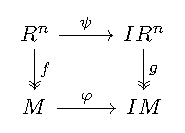
\includegraphics{lectures/3/commutative diagramms/GK.pdf}
 		\end{center}

 		Верхняя стрелка $\psi$ есть из универсального свойства свободного модуля. Так как каждый базисный элемент переходит в элемент с коэффициентами из $I$, $\psi \in M_{n}(I)$. Положим $p = \chi_{\psi}$. Тогда, так как $f$~--- сюръективно, $\forall m \in M \ \exists x\colon f(x) = m$. Тогда:
 		\[
 			p(\varphi)(m) = p(\varphi)(f(x)) = p(\psi)(g(x)) = 0 \implies p(\varphi) = 0.
 		\]
	\end{proof}

	\begin{theorem}[Лемма Накаямы]\label{Nakayama} 
		Пусть $M = IM$. Тогда $\exists a \in M\colon \forall m \in I \  am = m$
	\end{theorem}
	\begin{proof}
		$\id_{M}(M) = IM \implies $, а значит, по теореме Гамильтона-Кэли $\exists p(t) = t^n + \alpha_{n - 1}t^{n - 1} + \ldots + \alpha_0, \ \alpha_i \in I \colon p(\id_{M}) = 0$. Тогда 
		\[
			\id_{M}(1 + \alpha_{n - 1} + \ldots + \alpha_{0}) = 0 \implies \id_{M}(-(\alpha_{n - 1} + \ldots  + \alpha_0)) = 1.
		\]
		Тогда $a = -(\alpha_{n - 1} + \ldots  + \alpha_0)$ подходит. В самом деле, 
		\[
			am = \id_{M}(m) = m \quad \forall m \in M.
		\]
	\end{proof}

	\begin{corollary}
		Если $\varphi \in \End(M)$ и $\varphi$~--- эпиморфизм, то $\varphi$~--- изоморфизм. 
	\end{corollary}

	\begin{proof}
		Определим действие $R[t]$ на $M$ при помощи гомоморфизма $\theta$:
		\[
			\theta\colon R[t] \to \End(M) \quad \theta(t) = \varphi.
		\]

		Так как $\varphi$~--- эпиморфизм, $tR[t]M = M$. 

		Тогда по лемме Накаямы существует $f \in (t) = t R[t]$ такой, что $fm = m \ \forall m \in M$. Запишем $f = tg$ для некоторого $g \in R[t]$ и спроектируем результат в $\End(M)$:
		\[
			t g(t) \cdot m = m \implies \varphi(g(\varphi)(m)) = m \Leftrightarrow \varphi \circ g(\varphi) = \id.
		\]

		Но, по определению, $g(\varphi) = \varphi(g)$, тогда 
		\[
			g(\varphi)(\varphi(m)) = m,
		\]

		$g(\varphi)$~--- обратный к $\varphi$.
	\end{proof}

	\subsection{Радикал Джекобсона}

	Кольцо $R$, рассматриваемое, как модуль над собой, называется \emph{регулярным} $R$-модулем. 

	\begin{definition} 
		Аннулятором $R$-модуля $M$ называется множество $\{ r \in R \ \vert \ rM = 0 \}$.
	\end{definition}

	\begin{lemma} 
		Ненулевой простой $R$-модуль $M$ изоморфен $R/\fm$ для некоторого $\fm \in \Specm{R}$. Таким образом, $\Ann{M}$ является максимальным идеалом кольца $R$. 
	\end{lemma}

	\begin{proof} \ 
	\vspace{30mm}
	\end{proof}





    % Кольца дискретного нормирования 
    
	\subsection{Кольца нормирования, кольца дискретного нормирования и Дедекиндовы области}

	\begin{definition} 
		Пусть $R$~--- область целостности, $F$~--- её поле частных. $R$ называется \emph{кольцом нормирования}, если $R \cup (R \setminus 0)^{-1} = F$. То есть, $\forall x \in F$  либо $x \in R$, либо $x^{-1} \in R$.
	\end{definition}

	\begin{example}
		Например, кольцами нормирования являются $\Z_{(p)}, \ \Z_{p}, \ F[[x]]$. 
	\end{example}

	\begin{definition} 
		Пусть $F$~--- поле, а функция $\v\colon F^{*} \to \Gamma$, где $\Gamma$~--- линейно упорядоченная абелева группа, гомоморфизм, т.е. $\v(ab) = \v(a) + \v(b)$, причём выполнено 
		$\v(a + b) \ge \min(\v(a), \v(b))$ называется \emph{нормированием}.

		Если $\v$ действует в $\Z$ и сюръективна, то её называют \emph{дискретным нормированием} на $F$.
	\end{definition}

	Следующая теорема устанавливает связь между нормированием на поле и кольцами нормирования. 

	\begin{theorem} 
	\begin{enumerate}
		\item Пусть $\v$~--- нормирование на $F$, тогда $R \eqdef \{ x \in F \ \vert \ \v(x) \ge 0 \}$~--- кольцо нормирования.  	

		\item Если $R$~--- кольцо нормирования с полем частных $F$, то можно положить  $\Gamma = F^{*}/R^{*}$\footnote{в аддитивной записи\ldots} и задать на ней порядок следующим образом:
		\[
		 	aR^{*} \ge bR^{*} \Leftrightarrow ab^{-1} \in R.
		 \] 

		 и задать $\v\colon F^{*} \to F^{*}/R^{*}$. Тогда такое $\v$ будет нормированием. 

		 \item Процедуры из пунктов $(1)$ и $(2)$ взаимнообратны с точностью до изоморфизма на $\Im{\v}$ (как упорядоченных групп). 
	\end{enumerate}
	\end{theorem}
	\begin{proof}
		Докажем сначала (1):
		\[
			\v(x) + \v(x^{-1}) = 0 \implies \v(x) \ge 0 \text{ или }  \v(x^{-1}) \ge 0 \Leftrightarrow x \in R \text{ или } x^{-1} \in R.
		\]

		Теперь докажем $(2)$. Действительно, если $R$~--- кольцо номрирования, то либо $ab^{-1} \in R$, откуда $\v(a) \ge \v(b)$, либо $a^{-1}b \in R$, откуда $\v(b) \ge \v(a)$, то есть на $\Gamma = F^{*}/R^{*}$ порядок будет линейным. Кроме того, 
		\[
			\begin{cases} \v(a) \ge \v(b) \\ \v(b) \ge \v(a) \end{cases} \Leftrightarrow a b^{-1} \in R^{*} \Leftrightarrow aR^{*} = bR^{*} \Leftrightarrow \v(a) = \v(b),		\]
		что показывает антисимметричность. 

		Кроме того, $\v(a + b) \ge \v(a)$, либо $\v(a + b) \ge \v(b)$, откуда 
		\[
			\frac{a + b}{a} = 1 + \frac{b}{a} \in R, \text{  либо  } \frac{a + b}{b} = 1 + \frac{a}{b} \in R.
		\]

		Доказательство взаимной обратности остается в качестве простого \bf{упражнения}.
	\end{proof}

	\begin{statement} 
		Пусть $R$~--- кольцо нормирования, тогда $R$~---- локально и целозамкнуто. 
	\end{statement}
	\begin{proof}
		Положим $\fm \eqdef \{ a \in R \ \vert \ \v(a) > 0 \}$. Ясно, что $\forall x \in R, a \in \fm \ \v(ax) = \v(a) + \v(x) \ge \v(a) > 0$ и $\forall a, b \in \fm \ \v(a + b) \ge \min(\v(a), \v(b)) > 0$, что показывает нам, что $\fm$~--- идеал. Все остальные элементы имеют нормирвоание, равное нулю, и поэтому они обратимы (просто по определению), значит $\fm$~---  единственный максимальный идеал кольца $R$.  

		Теперь докажем целозамкнутость. Действительно, пусть $a \in F$
		\begin{multline*}
		  	a^n + r_{n - 1} a^{n - 1} + \ldots + r_0 = 0, \ r_i \in R \implies a^n = r_{n - 1}' a^{n - 1} + \ldots + r_0' \implies \v\lr*{\sum_{i = 1}^{n - 1} r_{i}' a^i} \ge \\ \ge \min\v\lr*{r_i' a^i} \ge \min{\v\lr*{a^i}} = \min(i \cdot \v(a)) \implies \v(a) \ge 0 \implies a \in R.
		\end{multline*}  
	\end{proof}

	\begin{statement}\label{DVR_Spec} 
		Пусть $R$~--- кольцо дискретного нормирования с нормированием $R$. Тогда 
		\begin{enumerate}
		 	\item $R \setminus \{ 0 \} \cong R^{*} \times \langle \pi \rangle$\footnote{тут имеется в виду изоморфизм моноидов. }

		 	\item $\Ideals(R) = \{0, R, \pi^n R, \text{ где } n \in \N \}$. 

		 	\item $\Spec{R} = \{ 0, \pi R\}$.

		 	\item $\Specm{R} = \{ \pi R \}$. 
		 \end{enumerate} 
	\end{statement}

	\begin{proof}
		Докажем сначала (1). Возмём $\pi\colon \v(\pi) = 1$ (мы можем так сделать, так как дискретное нормирование сюръективно). Возьмём $a \in R$, $\v(a) = n \in \Z \implies \v(a \pi^{-n}) = 0 \Leftrightarrow a \pi^{-n} \in R^{*} \Leftrightarrow a \in \pi^nR$ (причем очевидно, что такое представление единственно. 

		Рассмотрим $I \in \Ideals(R)$, возьмём $n = \min_{a \in I}{\v(a)} = \v(b) = \v(\pi^n \alpha)$, где $\alpha \in R^*$, а значит, $\forall c \in I\colon c = \pi^k \beta, \ k \ge n \implies c \in \pi^nR$. 
	\end{proof} 

	\begin{lemma}\label{Descanding_Filtration_By_Degrees_of_maximal_ideal} 
		Пусть $R$~--- нётерова область целостности, $\fm \in \Specm{R}, \ \fm \neq 0$, тогда $\fm^k \neq \fm^{k + 1} \ \forall k \in \N$.
	\end{lemma}
	\begin{proof}
		Рассмотрим $\fm^{k}/\fm^{k + 1}$~--- векторное пространство над $R/\fm$. Тогда 
		\[
			\fm^{k}/\fm^{k + 1} \otimes_{R} R_{\fm} \cong (\fm R_{\fm})^{k} / (\fm R_{\fm})^{k + 1} = 0 \implies \fm R_{\fm} (\fm^{k}R_{\rm}) = (\fm^{k}R_{\fm}) \implies \fm^k R_{\fm} = 0 \implies \fm = 0.
		\]
		В предпоследнем переходе мы используем лемму Накаямы (там конечнопорожденный модуль $\fm^{k} R_{\fm}$ умножается на $\fm R_{\fm} = \Rad(R_{\fm})$).
	\end{proof}

	\begin{theorem}\label{DVR_equiv} 
		Пусть $R$~--- область целостности. Тогда следующие условия эквивалентны: 
		\begin{enumerate}
			\item $R$~--- кольцо дискретного нормирования. 
			\item $R$~--- нётерово локальное целозамкнутое кольцо размерности Крулля 1. 
			\item $R$~--- локальное нётерово неполе, в котором максимальный идеал главный. 
			\item $R$~--- факториальное кольцо с единственным (с точностью до ассоциированности) неприводимым элементом. 
			\item Локальное неполе, идеалы которого имеют вид $\Ideals(R) = \{ 0, \fm^k \ \vert \ k \in \N_{0}\}$
		\end{enumerate}
	\end{theorem}
	\begin{proof}
		$(1) \implies (2)$ мы уже по сути доказали в утверждении~\ref{DVR_Spec}. Докажем теперь $(2) \implies (3)$. Мы знаем, что $\Specm{R} = \{ \fm \}$, возьмём $a \in \fm \setminus \fm^2$  по лемме~\ref{Descanding_Filtration_By_Degrees_of_maximal_ideal}. Рассмотрим $aR \subset \fm$. Из примарного разложения $aR$ следует, что $aR$~--- $\fm$-примарный. Тогда существует $k\colon \fm^{k} \subset aR \subset \fm$, выберем наименьшее из таких $k$. Теперь заметим, что 
		\[
			b \in \fm^{k - 1} \setminus aR \Leftrightarrow \frac{b}{a} \in \frac{\fm^{k - 1}}{a}
		\]

		\bf{\textcolor{red}{Дописать этот кусок.}}

		$(3) \implies (4):$ Возьмём $\pi \in R$~--- неприводимый, тогда $\pi \in \fm = aR$,  а значит, $\pi$~--- ассоциирован с $a$.

	\end{proof}



	

    % Дедекиндовы кольца 
    	
	\subsection{Дедекиндовы кольца}

	\begin{statement}\label{Dedekind_domain} 
		Пусть $R$~--- нётерова одномерная область целостности. Тогда следующие условия эквивалентны: 
		\begin{enumerate}
			\item $R$ целозамкнуто. 
			\item Любой примарный идеал имеет вид $\fm^k$ для некоторого $\fm \in \Specm{R}$.
			\item $\forall \fm \in \Specm{R}$ кольцо $R_{\fm}$~--- кольцо дискретного нормирования. 
		\end{enumerate}
	\end{statement}

	\begin{proof}
		$(1) \Leftrightarrow (3)$ просто в силу того, что целозамкнутость~--- локальное свойство и теоремы~\ref{DVR_equiv}. Ну и, в силу того, что $R_{\fm}$~--- нётеровы одномерные локальные. 

		$(3) \implies (2):$ В таком кольце любой ненулевой примарный идеал $I$ является $\fm$-примарным, а такие однозначно соотвествуют примарным идеалам локализации $R_{\fm}$. Так как $R_{\fm}$~--- $\mathrm{DVR}$, там все примарные идеалы имеют вид $\fm^n R_{\fm}$ (так как $R_{\fm}$~--- локальное кольцо с единственным максимальным идеалом $\fm R_{\fm}$), а $\lambda_*$~--- биекция на множестве примарных идеалов, не пересекающихся с мультипликативным подмножеством (которое тут $R \setminus \fm$, да), мы имеем $\lambda_*(I) = \lambda_*(\fm^n) \implies I = \fm^n$. 

		$(2) \implies (3):$ Любой идеал в $R_{\fm}$ имеет примарное разложение $\implies$ является примарным. $\lambda^{*}(J)$~--- $\fm$-примарный  $\implies \lambda^*(J) = \fm^n \implies \lambda_{*}(\lambda^*(J)) = \lambda_*(\fm^n) = (\fm R_{\fm})^n$, откуда по теореме~\ref{DVR_equiv} $R_{\fm}$~--- кольцо дискретного нормирования.  
	\end{proof}

	\begin{definition} 
		Кольца, удовлетворяющие условию~\ref{Dedekind_domain} называют \emph{дедекиндовыми}. 
	\end{definition}

	\begin{theorem} 
		Пусть $Z$~--- Дедекиндово кольцо, $Q$~--- его поле частных, $F/Q$~--- конечное расщирение (полей), а $R = \Int_{F}{Z}$. Тогда $R$~--- дедекиндово. 
	\end{theorem}

	\begin{proof}
		Так как $R$~--- целое замыкание, $\dim{R} = 1$. Так как $F$~--- конечное расширение, $\forall \alpha \in F$ является корнем многочлена 
		\[
			\alpha^n + \frac{a_{n - 1}}{b_{n - 1}}\alpha^{n - 1} + \ldots + \frac{a_0}{b_0} = 0, \quad a_i, b_i \in \Z \implies b \alpha^n + c_{n - 1} \alpha^{n - 1} + \ldots + c_0 = 0 \implies (b\alpha)^n + d_{n - 1} (b\alpha)^{n - 1} + \ldots + d_0 = 0
		\]
		Значит, $b\alpha \in R$, откуда $\alpha \in \lr*{Z \setminus 0}^{-1}R$.

		Так как $F$~--- поле частных $R$, $R$ целозамкнуто. Для дедекиндовости нам не хватает Нётеровости. 

		Рассмотрим $F$, как векторное пространство над $Q$. Рассмотрим оператор 
		\[
			m_{\alpha} \in \End_{Q-\fm \fo \fd}\lr*{F}, \ m_{\alpha}(x) = \alpha x.
		\]

		\emph{Далее доказательство приводится только для случая сепарабельного расширения}. 
		Так вот, если расширение сепарабельно, $\exists \alpha\in F \colon \Tr{m_{\alpha}} \neq 0$. Рассмотрим невырожденную билинейную форму $B(x, y) = \Tr{m_{xy}}\colon F \times F \to Q$.

		Возьмём базис $u_1, \ldots, u_n$~--- базис $F$ над $Q$ (можно полагать, что $u_i \in R$) и $v_1, \ldots, v_n$~--- двойственный базис относительно $B$. Возьмём $x \in F$, тогда 
		\[
			x = \sum_{k = 1}^{n} B(x, u_k) v_k.
		\]
		$x \in R, \ u_k \in R$, тогда $x u_k \in R$, а значит, его минимальный многочлен над $Q$ имеет коэффициенты из $Z$ (\textcolor{red}{была такая теорема, надо найти и вставить ссылку}). В то же время ясно, что минимальный многочлен $x u_k$ равен минимальному многочлену эндоморфизма $m_{x u_k}$. Собственные числа $m_{x u_k}$~--- это корни минимального многочлена, а они являются целыми над $Z$, следовательно и их сумма (с учетом кратности)~--- целая над $Z$, а это в точности след. Значит, $R$~--- подмодуль конечнопорожденного $Z$-модуля, а значит, так как $Z$~--- дедекиндово, $R$ конечнопорождено, как $Z$-модуль $\implies R$~--- нётерово.  
	\end{proof}

	В случае $Z = \Z$, кольцо $R$ называется дедекиндовым кольцом \emph{арифметического типа} или \emph{кольцом целых числового поля}. В случае $Z = K[t]$ кольцо $R$ называется дедекиндовым кольцом \emph{функционального} типа. 

	\subsection{Hauptidealsatz}

	\begin{definition} 
		Пусть $I$~--- идеал. Тогда  его \emph{высота} $\Ht(I)$~--- длина наибольшей цепочки вложенных в него простых идеалов. 
	\end{definition}

	\begin{theorem}[Крулль, о высоте]\label{hauptidealsatz}
	 	Пусть $x \in R$~--- нётерово коммутативное кольцо с единицей, $\fp$~--- минимальный простой идеал, содержащий $(x) = xR$. Тогда $\Ht(\fp) \le 1$. 	 
	 \end{theorem}  
	 \begin{proof}
	 	Во-первых, условие теоремы располагает к замене $R$ на $R_{\fp}$, т.е. далее будем считать, что $R$~--- локально с единственным максимальным идеалом $\fp$. Так что $\fp$~--- единственный минимальный простой, содержащий $xR$, а $xR$~--- $\fp$-примарным, откуда $\dim\lr*{R/xR} = 0$. Значит, $R/xR$~--- нульмерное нётерово, то есть Артиново. Действительтно, $\sqrt{xR} = \fp \implies \exists n \in \N \colon \fp^n = xR$, откуда $(\fp/xR)^n = 0$. Значит, если $p' \in \Spec{R/xR}$, то 
	 	\[
	 		\lr*{\fp/xR}^n \subset \fp' \subset \fp/xR \implies \fp/xR \subset \fp' \subset \fp/xR.
	 	\]

	 	\begin{definition} 
	 		Пусть $\fq \in \Spec{R}, \ \lambda = \lambda_{\fq}\colon R \to R_{\fq}$. Тогда \emph{символическая степень} идеала $\fq$ используется, как 
	 		\[
	 			\fq^{(n)} \eqdef \lambda^*\lr*{\lambda_*(\fq^n)}.
	 		\]
	 	\end{definition}

	 	\begin{lemma} 
	 		Идеал $\fq^{(n)}$~--- примарный. 
	 	\end{lemma}

	 	\begin{proof}
	 		$\lambda_{*}(\fq) \in \Spec{R_{\fq}} \implies \lambda_{*}(\fq^n) = \lambda_{*}(\fq)^n$~--- примарный, а $\lambda^*$ отображает примарные в примарные.  
	 	\end{proof}

	 	Пусть $\overline{\cdot}\colon R \to R/xR$~--- канонический гомоморфизм. Рассмотрим в $R/xR$ такую убывающую цепочку идеалов: 
	 	\[
	 		\overline{q} \supset \overline{\fq^{(2)}} \supset \ldots \supset \overline{\fq}^{(n)} = \overline{\fq}^{n + 1},
	 	\]
	 	так как $R/xR$~--- артиново. Возьмём $q^{(n)} \ni z = y + xr, \ y \in \fq^{(n + 1)}, r \in R$. Тогда $xr \fq^{(n)}$ и $x \notin \fq = \sqrt{\fq^{(n)}}$. Тогда отсюда следует, что $r \in q^{(n)}$


		Теперь $\fq^{(n)} = \fq^{(n + 1)} + x \cdot \fq^{(n)}$. Тогда в $R/\fq^{(n + 1)}$ мы имеем $\widetilde{x} \widetilde{q^{(n)}} = \widetilde{\fq^{(n)}}, \ \widetilde{x} \in \Rad{R/\fq^{(n + 1)}}$ и тогда по лемме Накаямы $\fq^{(n)} = 0$. 

		Значит, $\fq^{(n)} = \fq^{(n + 1)} \implies \lambda^{*}\lr*{\lambda_{*}(\fq^n)} = \lambda^*(\lambda_*(\fq^{n + 1})) \implies \lambda_*(\fq)^n = \lambda_*(\fq)^n \cdot \lambda_*(\fq)$, а $\lambda_*(\fq) \subset \Rad(R_{\fq})$ и тогда опять же по лемме Накаямы мы имеем $\lambda^*(\fq^n) = 0$. 

		Значит, $\Spec{R_{\fq}} = \{ \fq \} \implies $ в $R$ нет простых, содержащихся в $\fq \implies \Ht(\fq) = 0 \implies \Ht(\fp) \le 1$.  
	 \end{proof}
    % Пополнения
    
	\subsection{Пополнения}

	Пусть $A$~--- абелева группа с убывающей фильтрацией 
	\[
		A \supset A_0 \supset A_1 \supset \ldots A_n \supset
	\]

	$A$ можно сделать топологической группой, взяв в качестве базы окрестностей нуля $\{ A_n\}$. В нашем случае $A$ обычно будет кольцом или модулем, а фильтрация будет степенями идеала. 

	Ясно, что если $0 \neq a \in \bigcap A_i$, то её отделить от остальных не получится. Соотвественно, можно просто декларировать, что топология, заданная этой фильтрацией Хаусдорфова тогда и только тогда, когда 
	\[
		\bigcap_{i} A_i = 0. 
	\]

	Также заметим, что в этой топологии каждая $A_i$ будет не только открытой, но и замкнутой, так как все их сдвиги $x + A_i$ открыты, значит все смежные классы открыты и достаточно перейти к дополнению всех, кроме одного, откуда мы получим, что этот один смежный класс $y + A_j$ замкнут, следовательно $A_j$ замкнуто.

	Возьмём теперь пополнение по этой топологии. А именно, возьмём  прямой предел по следуюдщей последовательности: 
	\[
		\ldots \xrightarrow{\theta_2} A/A_2 \xrightarrow{\theta_1} A/A_1 \xrightarrow{\theta_0} A/A_0, \quad \widehat{A} \eqdef  \varprojlim A/A_{n}.
	\]

	\begin{definition} 
		Соотвественно, \emph{пополнением} $A$ в топологии, связанной с фильтрацией $\{ A_n \}$ называется определённое выше $\widehat{A}$.
	\end{definition}

	\begin{example}
		Например, $\Z_p = \varprojlim \Z/p^k\Z$ или $F[[t]] = \varprojlim F[t]/(t)^n$. 
	\end{example}

	Говорят, что фильтрации $(A_n)$ и $(B_n)$ имеют ограниченую разность, если 
	\[
		\exists n_0 \in \N \colon A_{n + n_0} \subset B_n \text{ и } B_{n + n_0} \subset A_n \ \forall \N.
	\]

	Ясно, что такие фильтрации задают одну и ту же топологию, но, на самом деле это условие сильнее (это мы поймём чуть попозже). 

	Напомним лемму о змее: 

	\begin{center}
		\textcolor{red}{сюда диаграмму про лемму о змее}
	\end{center}

	\begin{lemma} 
		Рассмотрим точную последовательность 
		\[
			0 \to A' \to A \to A'' \xrightarrow{p} 0, 
		\]
		$(A_n)$~--- фильтрация на $A$, $((A_n) \cap A')$~--- фильтрация на $A'$ и $(p(A_n))$ на A''. Тогда после перехода к пополнениям мы также получим точную последовательность 
		\[
			0 \to \widehat{A'} \to \widehat{A} \to \widehat{A''} \to 0.
		\]
	\end{lemma}
	\begin{proof}[Рабоче крестьянское доказательство] 
		Перейдём к точной последовательности: 
		\[
			0 \to A'/A_n \cap A' \to A/A_n \to A''/p(A_n)
		\]
		Определим теперь $\widetilde{A}$ и гомоморфизм $d$, как
		\[ 
			\widetilde{A} = \prod_{n = 0}^{\infty} A/A_n \xrightarrow{d} \widetilde{A}, \quad d((c_n)) = (c_n - \theta(c_{n + 1})). 
		\]

		Несложно заметить, что $\Ker{d} = \widehat{A}$. Соотвественно, надо рассмотреть диаграмму 
		\begin{center}
			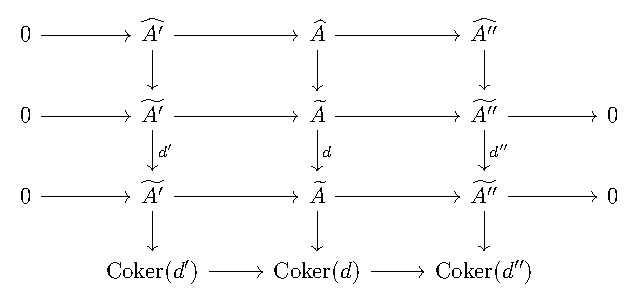
\includegraphics{lectures/3/commutative diagramms/snake_2.pdf}
		\end{center}

		и применить лемму о змее. Засчет сюръективности $\theta'$ $\ \forall (b_n)$ мы сможем подобрать $(c_n)$ такие, что $d'(c_n) = (b_n)$. А если $d'$ сюръективен, то $\Coker{d'} = 0$ и из леммы о змее мы получаем нужную  диаграмму:
		\[
			0 \to \widehat{A'} \to \widehat{A} \to \widehat{A''} \to \Coker{d'} = 0.
		\]

	\end{proof}
	\begin{proof}[Умновое доказательство]
		Оказывается, если существуют пределы $\lim{X_n}, \lim{Y_n}, \lim{Z_n}$ (где речь идет об объектах абелевой категории), то последовательность 
		\[
			0 \to \lim{X_n} \to \lim{Y_n} \to \lim{Z_n} 
		\]
		точна вообще всегегда, так как ядро~--- это предел, а пределы коммутируют, так как предельный функтор сопряжен к диагональному, а значит, сохраняет пределы. 
	\end{proof}

	\begin{corollary}
		$\widehat{A}/\widehat{A_n} \cong A/A_n$.
	\end{corollary}
	\begin{proof}
		Из прошлой леммы, полагая $A' = A_n$, мы получаем короткую точную последовательность 
		\[
			0 \to \widehat{A_n} \to \widehat{A} \to \widehat{A/A_n} \to 0
		\]

		А теперь заметим, что 
		\[
			(A/A_n) \supset A_1 / A_n \supset \ldots \supset A_n/A_n \supset 0 \supset \ldots, 
		\]
		откуда $\widehat{A/A_n} = A/A_n$ и из точности последоватльности выше мы получаем нужное. 
	\end{proof}

	\begin{corollary}
		Переходя в предыдущем следствии к пределу, мы получаем, что 
		\[
			\widehat{\widehat{A}} = \varprojlim \widehat{A}/\widehat{A_n} \cong \widehat{A},
		\]
		то есть пополение полно\footnote{что вполне логично. }
	\end{corollary}

	\begin{example}
		На простых примерах видна некоторая эвристика: $\Z \hookrightarrow \Z_{p}, \ F[t] \hookrightarrow F[[t]]$.
	\end{example}

	На самом деле, верно такое общее утверждение 
	
	\begin{theorem} 
		$\Ker\lr*{A \to \widehat{A}} = \bigcap_{n = 0}^{\infty} A_n$. 
	\end{theorem}

	\subsection{Градуированные алгебры и модули}

	\begin{definition} 
		Пусть $R_i$~--- $A$-модули. $R$ называют \emph{$\N$-градуированной $A$-алгеброй}, если 
		\[
			R = \bigoplus_{i = 0}^{\infty} R_i, \quad R_i \cdot R_j \subset  R_{i + j}.		
	 	\] 	

	 	\emph{Градуированным} $R$-модулем называют $M = \bigoplus M_i$ c условием $R_i M_j \subset M_{i + j}$.
	\end{definition}

	\begin{statement} 
		Градуированное кольцо $R$ является Нётеровым тогда и только тогда, когда $R_0$~--- нётерово и $R$~--- конечнопорожденная $R_0$-алгебра. 
	\end{statement}

	\begin{proof}
		В обратную сторону это почти очевидно: достаточно применить теорему Гильберта о Базисе и то, что нётеровость сохраняется при эпиморфизме. 

		Теперь докажем в обратную сторону.  Положим 
		\[
			R_{+} = \bigoplus_{n = 1}^{\infty} R_n \lei R,
		\]
		пусть $R_+$ порождён $\{ x_1, \ldots, x_s \}$  над $R$. Эти $x_i$ можно считать однородными, т.к. иначе разобьем на однородные компоненты, которые всё еще будут порождать. Таким образом, $x_i \in R_{k_i}$ для некоторого $k_i$. Возмём $y \in R_n$, 
		\[
			y = \sum_{j = 1}^{m} x_j z_j, \quad z_j \in R_{n - k_j}.
		\]

		По индукционному предположению $z_j \in R_0[x_1, \ldots, x_s] \implies y \in R_{0}[x_1, \ldots, x_s]$.
	\end{proof}

	Пусть $I \lei R$, расммотрим \emph{алгебру раздутия}: 
	\[
		\Bl_{I}\lr*{R} = \bigoplus_{n = 1}^{\infty} I^{n}. 
	\]
	







    \newpage

    \section{Алгебраическая теория чисел}
    % Тут я немножко факапнул с конспектом, так что лекции тут пока что что-то типа  с третьей. Остальное тоже допишу, обязательно.  

    % лекция 1: алгебраические числа, целые алгебраические числа 
    \subsection{Алгебраические числа и целые алгебраические числа}

	\begin{definition} 
		Число $\alpha \in \C$ называется \emph{алгебраическим}, если существует $p \in \Z[x]$, аннулирующий $\alpha$. 
	\end{definition}

	\begin{remark}
		Это частный случай общей терминологии, тут речь о том, что $\alpha$ алгебраичен над $\Q$.
	\end{remark}

	\begin{statement} 
		Пусть $\alpha \in \C$. Тогда следующие утверждения эквивалентны: 
		\begin{enumerate}
			\item $\alpha$~--- алгебраическое. 
			\item $\Q[\alpha]$~--- конечномерное векторное пространство над $\Q$.
		\end{enumerate}
	\end{statement}

	\begin{proof}
		$\mathbf{(1) \implies (2)}$: очевидно, так как если $\alpha$~--- алгебраичен над $\Q$,  базисом $\Q[\alpha]$ над $\Q$ будет множество $\{ 1, \alpha, \ldots, \alpha^{n - 1} \}$.

		$\mathbf{(2) \implies (1)}$: действительно, если $\dim_{\Q} \Q[\alpha] = n$, то $1, \alpha, \ldots, \alpha^n$ линейно зависимы, то есть $\exists a_0, \ldots, a_n \in \Q$:
		\[
			a_n \alpha^n + \ldots + a_1 \alpha + a_0 = 0.
		\]
		Домножая на знаменатель, мы имеем нужный многочлен. 
	\end{proof}

	\begin{statement} 
		Множество алгебраических чисел является полем. 
	\end{statement}
	\begin{proof}
		Пусть $\alpha$~--- алгебраическое число. Тогда 
		\[
			a_n \alpha^n + a_{n - 1}\alpha^{n - 1} + \ldots + a_1 \alpha + a_0 = 0, \ a_i \in \Z.
		\]
		Но тогда $a_n + \ldots + a_1 \lr*{\alpha^{-1}}^{n - 1} + a_0 \lr*{\alpha^{-1}}^{n} = 0$, то есть $\alpha^{-1}$ алгебраическое. Теперь, пусть $\alpha$ и $\beta$ алгебраические. Тогда 
		$\dim_{\Q}\Q[\alpha, \beta] < \infty \implies \dim_{\Q}\Q[\alpha \beta], \ \dim_{\Q}\Q[\alpha + \beta] < \infty$.    

	\end{proof}

	\begin{remark}
		Искушенный читатель сразу заметит, что это поле~--- это в точности $\Q^{alg}$.
	\end{remark}

	\begin{definition} 
		$\alpha \in \C$ мы будем называть \emph{целым алгебраическим числом}, если существует унитарный многочлен $p \in \Z[x]$, аннулирующий $\alpha$.
	\end{definition}

	\begin{example}
		$\sqrt{2}$~--- целое алгебраическое число, а вот $\sqrt{2}/2$~--- нет!
	\end{example}

	\begin{statement} 
		Следующие утверждения эквивалентны: 
		\begin{enumerate}
			\item $\alpha$~--- целое алгебраическое число. 
			\item $\Z[\alpha]$~--- конечно-порожденный $\Z$-модуль. 
		\end{enumerate}
	\end{statement}

	\begin{proof}
		Опять же, $\mathbf{(1) \implies (2)}$ следует просто из того, что если $\alpha$~--- целое алгебраическое, то $\{ 1, \ldots, \alpha^{n - 1} \}$~--- базис $\Z[\alpha]$ над $\Z$. 

		Теперь докажем $\mathbf{(2) \implies (1)}$. Ясно, что все образующие $\Z[\alpha]$ над $\Z$~--- многочлены от $\alpha$, пусть они $p_1(\alpha), \ldots, p_m(\alpha)$. Пусть $N = \max{\deg(p_i)}$, тогда 
		\[
			\alpha^{N + 1} = \sum_{i = 1}^{m} a_i p_i(\alpha), \quad \alpha^{N + 1} - \sum_{i = 1}^{m} a_i p_i(\alpha) = 0.
		\]
	\end{proof}

	\begin{theorem} 
		Множество целых алгебраических чисел является кольцом. 
	\end{theorem}
	\begin{proof}
		Возьмём $\alpha, \beta$~--- целые алгебраические. Тогда по предыдущему предложению $\Z[\alpha, \beta]$~--- конечнопорожденный $\Z$-модуль, а так как $\Z$~--- нётерово, тогда подумодули $\Z[\alpha + \beta]$ и $\Z[\alpha \beta]$ конечнопорождены, откуда $\alpha\beta$ и $\alpha + \beta$ целые алгебраические (также по предыдущему предложению). 
	\end{proof}

	Обозначим кольцо целых алгебраических чисел, как $\cO$. В основном в этом курсе мы будем изучать подкольца в $\cO$, а именно

	\begin{definition} 
		Пусть $K/\Q$~--- конечное расширение. Тогда 
		\[
			\cO_{K} \eqdef \cO \cap K
		\]
		мы будем называть \emph{кольцом целых} числового поля $K$. Иными словами, $\cO_{K}$~--- множество элементов $K$, для которых существует унитарный целочисленный многочлен, аннулирующий их. 
	\end{definition}

	\subsection{След элемента и целый базис кольца $\cO_{K}$}

	Заведём теперь некоторый полезный аппарат. 

	\begin{definition} 
		Пусть $L/K$~--- конечное расширение, $[L : K] = n$. Возьмём $\alpha \in L$, его можно рассматривать, как эндоморфизм понятным образом
		\[
			T_{\alpha}\colon L \to L, \quad x \mapsto \alpha x. 
		\]

		Соотвественно, след этого оператора называют следом элемента $\alpha$ относительно расширения $L/K$ и обозначают $\Tr_{L/K}(\alpha)$.

		У этого оператора есть характеристический многочлен $\chi_{\alpha}$. Выбрав базис $L/K$, мы можем записать матрицу оператора $T_{\alpha}$  и тогда 
		\[
			\chi_{\alpha}(t) = \det\lr*{Et - T_{\alpha}} = t^n - \Tr_{L/K}(\alpha)t^{n - 1} + \ldots 
		\]
		Если $L/K$~--- расширение Галуа, то можно определять след, как 
		\[
			\Tr_{L/K}(\alpha) = \sum_{\sigma \in \Gal(L/K)} \sigma(\alpha).
		\]
	\end{definition}

	Соотвественно, след~--- это $K$-линейный функционал $L \to K$, то есть 
	\[
		\forall \alpha, \beta \in K \quad \Tr_{L/K}(\alpha a + \beta b) = \alpha \Tr_{L/K}(a) + \beta \Tr_{L/K}(b).
	\]
	Кроме того, для $\alpha \in K$ $\Tr_{L/K}(\alpha) = [L : K] \cdot \alpha$. Кроме того, след хорошо ведёт себя относительно башни расширений. Если $M$~--- расширение $K$, а $K$~--- расширение $L$, то 
	\[
		\Tr_{M/K} = \Tr_{M/L} \circ \Tr_{L/K}.
	\]

	Кроме того, след можно рассматривать и как невырожденную билинейную симметричную форму 
	\[
		K \times K \to \Q, \ (x, y) \mapsto \Tr_{K/\Q}(xy).
	\]

	\begin{remark}
		Если $\alpha \in \cO_{K}$, то $\Tr_{K/\Q}(\alpha) \in \Z$. Действительно, во-первых, $\sigma(\alpha) \in \cO_k \ \forall \sigma \in \Gal(K/\Q)$, так как если $\alpha \in \cO_{K}$, то 
		\[
			\alpha^n + a_{n - 1} \alpha^{n - 1} + \ldots + a_0 = 0 \implies (\sigma\alpha)^n + a_{n - 1} (\sigma \alpha)^{n - 1} + a_0 = 0 \implies \sigma\alpha \in \cO_{K}
		\]

		, откуда $\Tr_{K/\Q}(\alpha) \in \cO_{K}$.

		С другой стороны, по первому определению $\Tr_{K/\Q} \in \Q$, а $\cO_{K} \cap \Q = \Z$. 
	\end{remark}

	\begin{statement}
		Любой элемент поля $K$ представим в виде $\frac{\beta}{d}$, где $\beta \in \cO_{K}$, $m \in \Z$. Иными словами, $K$~--- поле частных кольца $\cO_{K}$. 
	\end{statement}
	\begin{proof}
		Во-первых, $\alpha$ является корнем некоторого унитарного многочлена с коэффициентами из $\Q$:
		\[
			\alpha^n + c_{n - 1}\alpha^{n - 1} + \ldots + c_{1}\alpha + c_0 = 0, \quad c_i \in \Q.
		\]
		Запишем $c_i = \frac{b_i}{d}$, $b_i, d \in \Z$. Тогда, домножив равенство выше на $d^n$, мы получаем  
		\[
			(\alpha d)^n + b_{n - 1}(\alpha d)^{n - 1} + b_{n - 2} d (\alpha d)^{n - 2} + \ldots + b_0 d^{n - 1} = 0.
		\]
		Соотвественно, полагая $\beta = d\alpha$ мы видим, что $\beta \in \cO_{K}$ и $\alpha = \beta / d$. 
	\end{proof}

	Так вот, возьмём базис $K/\Q$. Из предыдущего предложения ясно, что можно полагать, что этот базис состоит из элементов $\cO_{K}$. Обозначим их за $\omega_1, \ldots, \omega_n$. Выберем для этого базиса взаимный базис $\omega_1^*, \ldots, \omega_n^*$ относительно формы $\Tr_{K/\Q}$, т.е. такой базис, что 
	\[
		\Tr(\omega_i \omega_j^*) = \begin{cases} 0, i \neq j \\ 1, i = j \end{cases} = \delta_{i j}.
	\]
	Покажем, что выполнено 
	\[
		\bigoplus_{i} \Z \omega_i \subset \cO_{K} \subset \bigoplus_{i} \Z \omega_i^{*}.
	\]

	Первое включение очевидно, докажем второе. Возмём $\alpha \in \cO_{K}$,
	\[
	 	\alpha = \sum_{i = 1}^{n} x_i \omega_i^{*}, \quad x_i \in \Q.
	 \] 
	 Покажем, что на самом деле $x_i \in \Z$. 
	 \[
	 	\alpha \omega_j = \sum_{i = 1}^{n} x_i \omega_j \omega_i^{*} \implies \Tr_{K/\Q}(\alpha \omega_j) = x_j. 
	 \]
	 С другой стороны, так как $\alpha \omega_j \in \cO_{K}$, $\Tr_{K/\Q}(\alpha \omega_j) \in \Z$ (как мы отвечали выше). Таким образом, мы имеем  
	 \[
		\bigoplus_{i} \Z \omega_i \subset \cO_{K} \subset \bigoplus_{i} \Z \omega_i^{*}.
	\]
	Так как слева и справа конечнопорождённые абелевы группы ранга $n$, мы только что доказали такую теорему: 

	\begin{theorem}\label{integral_basis_O_K} 
		Пусть $\cO_{K}$~--- кольцо целых числового поля $K/\Q$, где $K/\Q$~--- расширение степени $n$. Тогда, как абелева группа оно изоморфно конечнопорожденной свободной абелевой группе ранга $n$:
		\[
			\cO_{K} \cong \bigoplus_{i = 1}^{n} \Z u_i,
		\]
		где $\{ u_i \}$~--- базис $K/\Q$, состоящий из элементов кольца $\cO_{K}$. 

		В данном контексте $\{ u_i \}_{i = 1}^{n}$ называют \emph{целым базисом}. 
	\end{theorem}

	Из этой теоремы сразу следует вот такой факт:

	\begin{theorem} 
		Кольцо $\cO_{K}$~--- нётерово. 
	\end{theorem}
	\begin{proof}
		В самом деле, по теореме~\ref{integral_basis_O_K} кольцо $\cO_{K}$ конечно порождена, как абелева группа, а значит, любой его идеал $I \subset \cO_K$ тоже конечно порожден, как абелева группа, откуда следует, что он конечно порожден и как идеал. 
	\end{proof}

	\begin{example}\label{ring_of_integers_Q(sqrt(-3))}
		Рассмотрим поле $K = \Q(\sqrt{-3})$. Чему равно его кольцо целых $\cO_{K}$?

		Ясно, что $\Z[\sqrt{-3}] \subset \cO_{K}$, но вот равенства нет, так как можно рассмотреть 
		\[
			\alpha = \frac{1 + \sqrt{-3}}{2}, \quad 2\alpha - 1 = \sqrt{-3} \implies 4\alpha^2 - 4\alpha + 4 = 0 \implies \alpha^2 - \alpha + 1 = 0,		
		\]
		то есть $\alpha \in \cO_{K}$ и $\alpha \notin \Z[\sqrt{-3}]$. 
	

	Воспользуемся понятием \emph{нормы}:

	\begin{definition} 
		Пусть $L/K$~--- конечное расширение, $[L : K] = n$. Возьмём $\alpha \in L$, его можно рассматривать, как эндоморфизм понятным образом
		\[
			T_{\alpha}\colon L \to L, \quad x \mapsto \alpha x. 
		\]
		\emph{Нормой элемента $\alpha$ относительно расширения $L/K$} мы будем называть $\Nm_{L/K}(\alpha) = \Nm(\alpha) = \det(T_{\alpha})$. В случае, когда расширение сепарабельно, норму можно определять, как 
		\[
			\Nm(\alpha) = \prod_{\sigma \in \Gal(L/K)} \sigma(\alpha).
		\]
	\end{definition}

	\begin{remark}
		Как и в случае со следом, для $\alpha \in \cO_{K}$ $\Nm_{K/\Q}(\alpha) \in \cO_{K}$ (доказывается это так же, как для следа), а из определения через определитель ясно, что $\Nm_{K/\Q}(\alpha) \in \Q$, то есть $\Nm_{K/\Q}(\alpha) \in \Z$.
	\end{remark}

	Ясно, что в случае квадратичного расширения $\Q(\sqrt{d})$ норма $a + b\sqrt{d}$ норма элемента~--- произведение его на его сопряженный:
	\[
		\Nm(a + b\sqrt{d}) = (a + b\sqrt{d}))(a - b\sqrt{d}) = a^2 - d b^2
	\]

	Соотвественно, рассмотрим $a + b\sqrt{-3} \in \Q(\sqrt{-3})$ (т.е. $a, b \in \Q$) и пусть $\alpha = a + b\sqrt{-3} \in \cO_{K}$. Тогда 
	\[
		\Nm_{K/\Q}(a + b\sqrt{-3}) = (a + b\sqrt{-3})(a - b\sqrt{-3}) = a + 3b^3 \in \Z, \quad \Tr_{K/\Q}(a + b\sqrt{-3}) = (a + b \sqrt{-3}) + (a - b\sqrt{-3}) = 2a \in \Z. 
	\]

	Соответственно, $2a \in \Z$, то есть или $a = n/2$, где $n \in \Z$ и нечётное, или $a \in \Z$. 

	\begin{enumerate}
		\item Пусть $a \in \Z$, тогда так как $a^2 + 3b^2 \in \Z$, $3b^2 \in \Z \implies b \in \Z$. 

		\item Пусть $2a = 2n + 1$, тогда $4(a^2 + 3b^2) = 4a^2 + 12b^2 \in 4\Z \implies 12b^2 \in 4\Z$, откуда $2b \in \Z$. 
	\end{enumerate}

	Значит, либо $a$ и $b$ одновременно целые, либо $a$ и $b$ одновременно полуцелые. То есть 
	\[
	 	\alpha = \frac{2n + 1}{2} + \frac{2m + 1}{2}\sqrt{-3} = (n + m\sqrt{-3}) + \frac{1 + \sqrt{-3}}{2} = (n - m) + (2m + 1)\frac{1 +\sqrt{-3}}{2},
	 \] 
	 откуда $\cO_{K} \cong \Z \oplus \Z \cdot \frac{1 + \sqrt{-3}}{2}$.

	\end{example}

	\begin{example}
		Если $K = \Q(i)$, то $\cO_{K} = \Z[i]$.
	\end{example}

	\begin{homework}\label{hw_1}
		Задачи:
		\begin{enumerate}
			\item Опишите $\cO_{K}$ для $K = \Q(\sqrt{d})$, где $d \in \Z$ и $d$ свободно от квадратов. 

			\item Докажите, что любое конечное целостное кольцо является полем. 

			\item Рассмотрим поле $K = \Q(\sqrt{-5})$, $\cO_{K} = \Z[\sqrt{-5}]$ и идеал $I = (2, 1 + \sqrt{-5})$. Покажите, что он не является главным. 

			\item Докажите, что кольцо $\Z[\sqrt{-5}]$  не факториальное. А именно, рассмотрите
			\[
				21 = 3 \cdot 7 = (1 + 2\sqrt{-5})(1 - 2\sqrt{-5})
			\]
			и покажите: что это два существенно различных разложения в произвдение простых. 
		\end{enumerate}
	\end{homework}

	\subsection{Размерность кольца целых $\cO_{K}$}

	Докажем теперь, что для любого числового поля $K$ кольцо целых $\cO_{K}$ одномерно. 

	\begin{lemma}\label{integer_in_ideal_of_O_K} 
		Пусть $K/\Q$~--- конечное расширение и  $0 \neq I$~--- идеал кольца $\cO_{K}$. Тогда $I \cap \Z \neq 0$, то есть $I$ содержит целое число. 
	\end{lemma}

	\begin{proof}
		Возьмём $\alpha \in I$, $\alpha \neq 0$. Тогда 
		\[
			\alpha^n + a_{n - 1} \alpha^{n - 1} + \ldots + a_{1}\alpha + a_0 = 0, \quad a_i \in \Z.
		\]
		Не умаляя общности, $a_0 \neq 0$. Но тогда 
		\[
			a_0 = - (\alpha^n + a_{n - 1} \alpha^{n - 1} + \ldots + a_{1}\alpha) \implies a_0 \in \Z \cap I.
		\]
	\end{proof}

	\begin{corollary}\label{O_K/I}
		Пусть $I$~--- ненулевой идеал в $\cO_{K}$. Тогда $\cO_{K}/I$ конечно. 
	\end{corollary}
	\begin{proof}
		По лемме~\ref{integer_in_ideal_of_O_K} выберем $n \in I \cap \Z$, $n \neq 0$. Тогда 
		$(n) = n\cO_{K} \lei I$, значит достаточно доказать, что $\cO_{K}/n\cO_{K}$ конечно. А это сразу же следует из того, что $\cO_{K}$~--- это конечнопорожденная свободная абелева группа ранга $n$. 
	\end{proof}
	
	\begin{theorem} 
		Кольцо $\cO_{K}$ одномерно, т.е. $\dim(\cO_{K}) = 1$. 
	\end{theorem}

	\begin{proof}
		Пусть $\fp \in \Spec(\cO_{K})$. Тогда $\cO_{K}/\fp$~--- область целостности и конечно по  следствию~\ref{O_K/I}. Но тогда по задаче 2 в~\ref{hw_1} $\cO_{K}/\fp$~--- поле, что равносильно тому, что $\fp$~--- максимальынй. 
	\end{proof}

	\begin{remark}
		Эквивалентная формулировка этой теоремы состоит в том, что любой ненулевой простой идеал  кольца $\cO_{K}$ является максимальным. 
	\end{remark}

	Поговорим теперь еще про строение идеалов в кольце $\cO_{K}$. Как мы уже убеждались в задаче 3 Д/З~\ref{hw_1}, кольцо $\cO_{K}$ далеко не всегда является областью главных идеалов. 

	\subsection{Примеры евклидовых колец целых алгебраических чисел}

	\begin{statement} 
		Рассмотрим $K = \Q(\sqrt{-3})$. Тогда $\cO_{K}$~--- евклидово. 
	\end{statement}

	\begin{proof}
		Как мы убедились в примере~\ref{ring_of_integers_Q(sqrt(-3))}, 
		\[
			\cO_{K} \cong \Z \oplus \Z \omega, \quad \omega = \frac{1 + \sqrt{-3}}{2}. 
		\]
		Рассмотрим $a + b \omega$, тогда  положим
		\[
			\Nm(\alpha) = (a + b\omega)(a + b\overline{\omega}) = a^2 + ab + b^2.
		\]

		Пусть $a, b, c, d \in \Z$, тогда
		\[
			\frac{a + b\omega}{c + d\omega} = \alpha + \beta \omega, \quad \alpha, \beta \in \Q.
		\]

		Тогда существуют $u, v \in \Z$ такие, что $|u - \alpha| \le \frac{1}{2}$, $|v - \beta| \le \frac{1}{2}$. Положим $\alpha - u = \alpha'$, $\beta - v = \beta'$.

		\[
			a + b\omega = (c + d\omega)(\alpha + \beta \omega) = (c + d\omega)(u + v\omega) + (c + d\omega)(\alpha' + \beta' \omega) = (c + d \omega)(u + v \omega)  + r.
		\]
		\[
			\Nm(r) = \Nm((c + d\omega)(\alpha' + \beta' \omega)) = \Nm(c + d \omega)\Nm(\alpha' + \beta' \omega) = \Nm(c + d\omega)(\alpha'^2 + \alpha'\beta' + \beta'^2) < \Nm(c + d \omega),
		\]
		так как $\alpha'^2 + \alpha'\beta' + \beta'^2 \le \frac{1}{4} + \frac{1}{4} + \frac{1}{4} = \frac{3}{4}$, что и требовалось. 
			
	\end{proof}

	Сейчас мы посмотрим 
	\begin{statement} 
		Уравнение $y^2 = x^3 - 2$ над $\Z$ в качестве решений имеет лишь $(3, \pm 5)$.
	\end{statement}
	\begin{proof}
		Во-первых заметим, что можно сразу полагать $y$ нечётным. 

		Попробуем решить уравнение в $\Z[\sqrt{-2}] = \cO_{K}$ для $K = \Q(\sqrt{-2})$. 
		\[
			(y + \sqrt{-2})(y - \sqrt{-2}) = x^3.
		\]
		Пусть $d = (y + \sqrt{0-2}, y - \sqrt{-2})$. Покажем, что $d = 1$. Действительно, 
		\[
			\begin{cases} y + \sqrt{-2} \divby d \\ y - \sqrt{-2} \divby d \end{cases}	\implies \begin{cases} 2y \divby d \\ 2\sqrt{-2} \divby d \end{cases}.
		\]	
		Заметим, что $2\sqrt{-2} \divby d \implies \Nm(2 \sqrt{-2}) \divby \Nm(d)$. Пусть $d = a + b \sqrt{-2}, \ a, b \in \Z$. Тогда  мы имеем $8 \divby (a^2 + 2b^2)$. 
		
		Т.е. $a^2 + 2b^2 = 1, 2, 4$ или 8. Разберём соотвествующие случаи: 
		\begin{enumerate}
			\item $a^2 + 2b^2 = 1  \rightsquigarrow a = \pm 1,\  b = 0$. 

			\item $a^2 + 2b^2 = 2 \rightsquigarrow a = 0, \ b = \pm 1$. 

			\item $a^2 + 2b^2 = 4 \rightsquigarrow a = \pm 2, \ b = \pm 0$. 

			\item $a^2 + 2b^2 = 8 \rightsquigarrow a = \pm 0, \ b = \pm 2$. 
		\end{enumerate}

		Заметим, что так как $y$~--- нечётное целое, 
		\[
			\Nm(y + \sqrt{-2}) = y^2 + 2 \notdivby \Nm(\sqrt{-2}) = 2,
		\]
		откуда следует, что случаи $(2)$ и $(4)$ нам не годятся. Случай $(3)$ нам не подходит просто в силу того, что $y$ нечётное. 

		Значит, мы доказали, что $y + \sqrt{-2}$ и $y - \sqrt{-2}$~--- взаимнопросты, а так как кольцо $\Z[\sqrt{-2}]$ факториально, отсюда мы имеем, что 
		\[
			y + \sqrt{-2} = z^3, \quad y - \sqrt{-2} = t^3. 
		\]
		Пусть опять же $z = a + b \sqrt{-2}$. Честно возведём в куб: 
		\[
			y + \sqrt{-2} = (a + b\sqrt{-2})^3 = a^3 + 3a^2 b \sqrt{-2} - 6 a b^2 - 2 b^3 \sqrt{-2},
		\]
		октуда мы имеем 
		\[
			\begin{cases} a^3 - 6ab^2 = y \\ 3a^2 b - 2b^3 = 1 \end{cases}
		\]
		Соотвественно, из второго уравнения ясно, что $b = \pm1$, откуда либо $3a^2 = 3 \implies a = \pm 1$, либо $3a^2 = -1$, чего быть не может ($a \in \Z$). Соотвественно, мы получили, что 
		\[
			y = a^3 - 6ab^2 = \pm 5 \implies y = \pm 5.
		\]
	\end{proof}







    % лекция 2:
    \textcolor{red}{Вот тут началась лекция 2, её пока что тут нет}
    % лекция 3: разложение идеалов в произведение простых в колцье \cO_{K}
    	\subsection{Разложение идеалов в произведение простых в кольцах целых числовых полей}

	\begin{lemma}\label{prime_ideals_product_lemma}
		Пусть $A$~--- нётерово, $I \subset A$~--- ненулевой идеал. Тогда существуют такие простые идеалы $\fp_{1}, \ldots, \fp_{k}$, что $\fp_{1} \fp_{2} \ldots \fp_{k} \subset I$.
	
	\end{lemma}

	\begin{proof}
		Предположим противное, то есть, что существуют идеаы, для которых не выполнено условие леммы. Выберем среди таких максимальный (мы можем так сделать в силу нётеровости кольца), назовём его $I$. Заметим, что $I$~--- не простой идеал, что означает, что $\exists x, y\colon \notin I\colon xy \in I$. Кроме того, $I$~--- собственный идеал. Значит, 
		\[
			I + (x) \supset (x), \quad I + (y) \supset I,
		\]
		причем включение строгое. Тогда для идеалов $I + (x)$ и $I + (y)$ условие леммы уже выполняется, то есть $\exists \fp_{1}, \ldots, \fp_{k}$ и $\fq_{1}, \ldots, \fq_{m}$ такие, что $\fp_{1}\ldots \fp_{k} \subset I + (x)$, $\fq_{1} \ldots \fq_{m} \subset I + (y)$.
		Но тогда мы имеем 
		\[
			\fp_{1}\ldots\fp_{k}\fq_{1}\ldots\fq_{m} \subset (I + (x))(I + (y)) \subset I, \text{ так как } xy \in I,
		\]
		что даёт нам противоречие. 
	\end{proof}


	\begin{definition} 
		Пусть $K/\Q$~--- конечное расширение, $0 \neq I \subset \cO_{K}$~--- идеал. Тогда введём 
		\[
			I^{-1} \eqdef \{ x \in K \ \vert \ xI \subset \cO_{K} \}.
		\]
	\end{definition}

	\noindent\bf{Свойства:}

	\begin{enumerate}
		\item $x, y \in I^{-1} \implies x + y \in I^{-1}$.
		
		\item Если $x \in I^{-1}$, а $a \in \cO_{K}$, то $ax \in I^{-1}$.
	\end{enumerate}
	\begin{proof}
			Действительно, $(x + y)I \subset xI + yI \subset \cO_{K}$. Если $xI \subset \cO_{K}$, то для $a \in \cO_{K}$
			мы получим $axI = xaI = xI$, так как $I$~--- идеал в $\cO_{K}$.
		\end{proof}

	\begin{remark}
		Заметим, что $I^{-1}$~--- $\cO_{K}$-модуль. Кроме того, если $a \in I$, то $aI^{-1}$~--- идеал в $\cO_{K}$.
		В частности, $aI^{-1}$ конечнопорожден,  а значит, $aI^{-1}$~--- конечнопорожденный $\cO_{K}$-модуль. 
	\end{remark}

	\begin{example}
		Пусть $K = \Q,$ тогда $\cO_{K} = \Z$ и любой идеал $I \subset \Z$ имеет вид $I = (a)$. Тогда $(a)^{-1} = a^{-1}\Z$.
	\end{example}

	\begin{lemma}\label{frac_ideal_is_not_ring}
		Пусть $I \subset \cO_{K}$~--- ненулевой собственный идеал. тогда $I^{-1} \neq \O_{K}$.
	\end{lemma}

	\begin{proof}
		Докажем, что существуует $x \in K$ такой, что $x \notin \cO_{K}$ и при этом $xI \in \cO_{K}$.
		Выберем в $I$ ненулевой элемент $a$. Рассмотрим $(a) \subset I$, по лемме~\ref{prime_ideals_product_lemma} найдутся такие ненулевые 
		$\fp_{1}, \ldots, \fp_{k} \in \Spec{\cO_{K}}$, что $\fp_{1}\ldots\fp_{k} \subset (a)$. 

		Так как $I$~--- собственный, а кольцо $\cO_{K}$ одномерно, $I$ лежит в некотором простом идеале $\fp$. Так мы получаем цепочку включений 
		\[
			\fp_{1}\ldots \fp_{k} \subset (a) \subset \fp \implies \ \exists i\colon \fp_{i} \subset \fp.
 		\]
 		Так как оба идеала максимальны, это не включение, а равенство. Не умаляя общности, пусть $\fp_{1} = \fp$. Теперь, пусть $k = 1$. 
 		Тогда мы имеем $\fp \subset (a) \subset  I \subset \fp \implies I = \fp = (a) \implies I^{-1} = a^{-1}\cO_{K}$. 
 		Значит, $x = a^{-1} \notin \cO_{K}$, так как иначе $I = \cO_{K}$. 

 		Теперь пусть $k \ge 2$, выберем $k$ минимально возможным.  Тогда 
 		\[
 			\fp_{2}  \ldots \fp_{k} \not\subset (a) \implies \exists b \in \fp_{2}\ldots \fp_{k} \setminus (a).
 		\]
 		Тогда мы можем взять $x = \frac{b}{a}$ и тогда $xI = \frac{b}{a}I \subset \frac{b}{a}\fp_{1} \subset \frac{\fp_{1}\ldots \fp_{k}}{a} \subset \frac{(a)}{a} = \cO_{K}$. Остаётся проверить, что $\frac{b}{a} \notin \cO_{K}$.В самом деле, если $\frac{b}{a} \in \cO_{K}$, то $b \in (a)$, что противоречит выбору $b$.
	\end{proof}

	\begin{remark}
		Ясно, что включение $\cO_{K} \subset I^{-1}$ верно всегда, так как просто по определению идеала $\forall x \in \cO_{K} \ xI \subset \cO_{K}$
	\end{remark}

	Возьмём $\fp \in \Spec{\cO_{K}}$ и рассмотрим $\fp \fp^{-1}$. С одной стороны, это идеал в $\cO_{K}$, причём он содержит $\fp$.

	\begin{lemma}\label{p p^{-1} = (1)} 
		Пусть $\fp \in \Spec{\O_{K}}$, тогда $\fp \fp^{-1} = (1) = \cO_{K}$.
	\end{lemma}
	\begin{proof}
		Предположим противное, тогда в силу максимальности идеала $\fp$ мы имеем $\fp \fp^{-1} = \fp$. 
		Пусть $\fp = (u_{1}, \ldots, u_{n})$, тогда если $\alpha \in \fp^{-1} \setminus \cO_{K}$ (тут мы пользуемся леммой~\ref{frac_ideal_is_not_ring}), то $\alpha u_{1} \in \fp$ и мы можем написать систему уравнений 
		\[
			\begin{cases} \alpha u_{1} = \sum\limits_{u = 1}^{n} a_{1 i} u_{i}   \\
			\alpha u_{2} = \sum\limits_{u = 1}^{n} a_{2 i} u_{i} \\ 
			\vdots \\ 
			\alpha u_{n} = \sum\limits_{i = 1}^{n} a_{n i} u_{i} \end{cases}
		\]
		В матричной форме эта система будет иметь вид 
		\[
			\underbrace{\begin{pmatrix} \alpha - a_{11} & \ldots & \ldots & \ldots \\ \ldots & \alpha - a_{22} & \ldots & \ldots \\ \vdots & \vdots & \ddots & \vdots \\ \ldots & \ldots & \ldots & \alpha - a_{nn} \end{pmatrix}}_{= B} \cdot \begin{pmatrix} u_{1} \\ u_{2} \\ \vdots \\ u_{n} \end{pmatrix} = 0.
		\]
		Значит, $\det{B} = 0$, что даёт нам унитарный многочлен с коэффициентами из $\cO_{K}$, обнуляющий $\alpha$. Тогда, так как $\cO_{K}$~--- целозамкнуто, $\alpha \in \cO_{K}$, противоречие. 
	\end{proof}

	Теперь мы достаточно подготовились, чтоб доказать, что в кольце $\cO_{K}$ любой идеал раскладывается в произведение простых единственным образом. 

	\begin{theorem}[О разложении идеалов в произведение простых]\label{ideal_factorization}
		Пусть $0 \neq I \subset \cO_{K}$~--- идеал. Тогда $I$ однозначно (с точностью до перестановки сомножителей) раскладывается в произведение простых идеалов. 
	\end{theorem}

	\begin{proof} Как обычно, проходит в два этапа. \\
		\emph{Существование:} Предположим, что существуют идеалы, не раскладывающиеся в произведение простых. Среди таких идеалов возьмём максимальный, обозанчим его $I$ (мы можем так сделать, потому что $\cO_{K}$~--- нётерово кольцо). Он содержистся в некотором максимальном идеале $\fp \in \Specm{\cO_{K}}$. Тогда $I \fp^{-1} \subset \fp \fp^{-1} = \cO_{K}$~--- идеал. Значит, нам остаётся показать, что $I \fp^{-1} \neq I$. Покажем, что $I I^{-1} = \cO_{K}$, тогда мы сможем просто домножить и всё получистя. 

		\begin{lemma} 
			Для любого идеала $I \subset \cO_{K}$ мы имеем $I I^{-1} = \cO_{K}$. 
		\end{lemma}

		\begin{proof}
			Пусть это не так, тогда $I I^{-1} \subset \fq$, где $\fq$~--- максимальный идеал. Тогда $I I^{-1} \fq^{-1} \subset \fq \fq^{-1} = \cO_{K} \implies  I^{-1}\fq^{-1} \subset I^{-1}$. Так как $\fq^{-1}$ не совпадает с $\cO_{K}$, мы можем выбрать $\alpha \in \fq^{-1}\setminus \cO_{K}$. Проделывая рассуждение, аналогичное лемме~\ref{p p^{-1} = (1)} мы получаем, что $\alpha \in \cO_{K}$, что даёт нам противоречие. 
		\end{proof}

		Итак, если $I \fp^{-1} = I$, то $\fp^{-1} = \cO_{K}$, что противоречит лемме~\ref{frac_ideal_is_not_ring}. Значит, $I \subset I\fp^{-1} $, следовательно мы можем разложить $I \fp^{-1}$ в произведение простых:
		\[
			I \fp^{-1} = \fp_{1} \fp_{2} \ldots \fp_{k} \implies I = \fp_{1} \fp_{2} \ldots \fp_{k} \cdot \fp, 
		\]
		что и требовалось. \\
		\emph{Единственность:} Пусть $\fp \fp_{1} \ldots \fp_{m} = \fp \fq_{1} \ldots \fq_{n}$, тогда $\fp_{1} \fp_{2} \ldots \fp_{m} \subset \fq_{1} \implies \ \exists i\colon \fp_{i} \subset \fq_{i}$, а так как они максимальны, $\fp_{i} = \fq_{1}$, что даёт нам противоречие. 
	\end{proof}

	\begin{definition} 
		Пусть $I \subset K$. $I$ называется \emph{дробным идеалом}, если $\exists x \neq 0\colon x I \subset \cO_{K}$~--- идеал.
	\end{definition}

	\begin{example}
		$I^{-1}$~--- дробный идеал. 
	\end{example}

	\begin{statement} 
		Ненулевые дробные идеалы образуют группу по умножению. 
	\end{statement}

	\begin{proof}
		Легко заметить, что произведение дробных идеалов~--- дробный идеал. Обратный определяется как и раньше:
		\[
			I^{-1} \eqdef \{ x \in K \ \vert \ xI \subset \cO_{K} \}.
		\]
		Нетрудно убедиться в том, что $I I^{-1} = \cO_{K}$. 
	\end{proof}

	Из теоремы~\ref{ideal_factorization} следует, что любой дробный идеал раскладывается в произведение простых идеалов (возможно, с отрицательными степенями). Действительно, пусть $J$~--- дробный идеал, тогда для некоторого $x \in K \ xJ = I$~--- идеал в $\cO_{K}$, тогда 
	\[
		J = (x)^{-1}I = \fp_{1}^{-1} \ldots \fp_{k}^{-1} \fq_{1}\ldots \fq_{m}.
	\]

	Значит, группа дробных идеалов~--- свободная абелева группа, образующие которой~--- элементы $\Spec{\cO_{K}}$.

	\begin{example}
		Для кольца $\Z$ дробные идеалы соотвествуют рациональным числам. 
	\end{example}


	



	
    % лекция 4: дискриминант в числовых полях и его приложения. 
    
	\subsection{Дискриминант}

	\begin{definition}\label{discriminant} 
		Пусть $K/F$~--- конечное сепарабельное расширение, $[K : F] = n$ и $\alpha_1, \ldots, \alpha_n \in K$.
		Тогда \emph{дискриминант} набора $\alpha_1, \ldots, \alpha_n$~--- это 
		\[
			\disc(\alpha_1, \ldots, \alpha_n) \eqdef \det\lr*{\Tr_{K/F}(\alpha_i \alpha_j)}.
		\]
	\end{definition}
		Так как расширение $K/F$ сепарабельно, у нас есть ровно $n = [K : F]$ вложений $\sigma_1, \ldots, \sigma_n\colon K \to \C$ (на самом деле, мы знаем, что в  $\Q^{alg}$).

		\begin{statement}\label{disc_prop_1} 
			$\disc(\alpha_1, \ldots, \alpha_n) = \lr*{\det(\sigma_{i}(\alpha_j)}^{2}$.	
		\end{statement}
		\begin{proof}
			Положим $(\sigma_{i}(\alpha_j))_{i,j = 1}^{n} = A$ и рассмотрим $A^{t} A$, тогда 
			\[
				(A^{t} A)_{i j} = \sum_{k = 1}^{n} \sigma_{k}(\alpha_i) \sigma_k(\alpha_j) = \sum_{k = 1}^{n} \sigma_{k}(\alpha_i \alpha_j) = \Tr_{K/F}(\alpha_i \alpha_j).
			\]
		\end{proof}

		Посмотрим теперь, как дискриминант меняется при линейном преобразовании. Пусть $(\beta_1, \ldots, \beta_n) = (\alpha_1, \ldots, \alpha_n)M, \ M \in M_{n}(F)$.

		\begin{statement}\label{disc_prop_2} 
			$\disc(\beta_1, \ldots, \beta_n) = \disc(\alpha_1, \ldots, \alpha_n) \cdot \lr*{\det{M}}^{2}$.
		\end{statement}
		\begin{proof}
			Действительно, это напрямую следует из предложения~\ref{disc_prop_1}:
			\[
			 	\disc(\beta_1, \ldots, \beta_n) = \det\lr*{\sigma_{i}(\beta_{j})}^{2} = \det{\lr*{\sigma_{i}(\alpha_{j})M}}^2 = \disc(\alpha_1, \ldots, \alpha_n) \cdot \lr*{\det{M}}^{2}. 
			 \] 
		\end{proof}

		\begin{statement} 
			$\disc(\alpha_1, \ldots, \alpha_n) = 0 \Leftrightarrow \alpha_1, \ldots, \alpha_n$~--- линейно зависимы. 
		\end{statement}
		\begin{proof}
			Пусть $\alpha_1, \ldots, \alpha_n$~--- линейно зависимы, $e_1, \ldots, e_n$~--- базис $K/F$. Тогда
			\[
				(\alpha_1, \ldots, \alpha_n) = (e_1, \ldots, e_n)M, \quad \det{M} = 0.
			\]
			Значит, по предложению~\ref{disc_prop_2} мы имеем $\disc(\alpha_1, \ldots, \alpha_n) = 0$. 

			Теперь докажем в обратную сторону. 
			Предположим, что $\alpha_1, \ldots, \alpha_n$~--- линейно независимы, но $\disc(\alpha_1, \ldots, \alpha_n) = \det\lr*{\Tr_{K/F}(\alpha_i \alpha_j)} = 0$. Рассмотрим систему линейных уравнений 
			\[
				\Tr_{K/F}\lr*{(x_1 \alpha_1 + \ldots + x_n \alpha_n)\alpha_j} = 0, \ldots 1 \le j \le n.
			\]
			Так как матрица коэффициентов этой системы~--- $\Tr_{K/F}(\alpha_i \alpha_j)$, а она вырождена, система имеет нетривиальное решение $(x_1, \ldots, x_n)$. Так как $\alpha_1, \ldots, \alpha_n$~--- линейно независимы, 
			\[
				y = x_1 \alpha_1 + \ldots +  x_n \alpha_n \neq 0.
			\]

			С другой стороны, $\Tr_{K/F}(y \alpha_{j}) = 0 \ \forall j$. Так как $\alpha_i$ образуют базис $K/F$, по линейности мы получаем, что $\Tr_{K/F}(y u) = 0 \ \forall u \in K$. Но, так как расширение $K/F$ сепарабельно, $\Tr_{K/F}$ должен быть невырожденной формой\footnote{Этим утверждением из теорией полей мы пользуемся без доказательств. Доказательство этого утверждения можно прочитать в S. Lang ``Algebra''. }.
			

		\end{proof}

		\begin{lemma}\label{free_abelian_groups_prop} 
			Пусть $B \subset A$~--- свободные абелевы группы ранга $n$. Пусть $\omega_1, \ldots, \omega_n$~--- базис $A$, а $\left\{\sum_{j = 1}^{n} a_{i j} w_{j}\right\}$~--- базис $B$, $a_{i j} \in \Z$. Тогда $|A / B| = |\det(a_{i j})|$.
		\end{lemma}
		\begin{proof}
			Приведём матрицу $(a_{i j})$ нормальной форме Смита. Перечислим теперь элементы $A/B$: это в точности элементы $x_1 \omega_1 + \ldots + x_n \omega_n, \ 0 \le x_i \le a_{ii} - 1$. Если мы докажем, что это в точности все попарно-различные элементы группы $A/B$, то утверждение будет ясно. 

			Пусть $\sum_{i = 1}^{n} x_i \omega_i = \sum_{i = 1}^{n} y_i \omega_i$, тогда $\sum_{i = 1}^{n}(x_i - y_i) \omega_i \in B$. Посмотрим на коэффициент при $\omega_{11}$, он может получаться только из первой строки матрицы (так как матрица верхнетреугольная), тогда   $\ell a_{11} = x_{1} - y_{1}$, но это равенство возможно только в случае, когда $x_1 = y_1$ (так как есть ограничения на $x_i$ и $y_i$). Далее мы проделаем аналогичное рассуждение $\sum_{i = 2}^{n} (x_i - y_i) \omega_i \in B$ и в итоге получим, что все такие элементы разлчины. 

			Теперь рассмотрим $a = x_1 \omega_1 + \ldots + x_n \omega_n, \ x_i \in \Z$. Поделим с остатком: $x_1 = a_{11}q + r, \ 0 \le r  < a_{11}$, и рассмотрим $x_{1} \omega_{1} + \ldots + x_n \omega_n - q(a_{11}\omega_1 + \ldots + a_{1n}\omega_n) = r\omega_1 + x_{2}'\omega_{2} + \ldots$.  Так как мы вычли из $a$ элемент из $B$, класс $\overline{a} \in A/B$ не изменился, а старшим коэффициентом стал $r$, лежащий в нужном диапазоне. Продолжая в том же духе, мы полчми, что все коэффициенты лежат в нужном диапазоне. 
		\end{proof}

		Как мы помним из теоремы~\ref{integral_basis_O_K}, $\cO_{K}$~--- конечнопорожденная свободная абелева группа ранга $n = [K : \Q]$ и $\cO_{K} = \bigoplus_{i = 1}^{n} \Z \omega_{i}$, где $\{ \omega_i \}$~--- целый базис. 

		\begin{definition} 
			Пусть $K/\Q$~--- расширение степени $n$,  $\cO_{K} = \bigoplus_{i = 1}^{n} \Z \omega_{i}$. Тогда 
			\[
				\disc(K) \eqdef \disc\lr*{\omega_{1}, \ldots, \omega_{k}}.
			\]
		\end{definition}
	
		\begin{remark}
			Дискриминант поля не зависит от выбора целого базиса. Действительно, если у нас есть какой-то другой целый базис $(u_1, \ldots, u_n)$, то 
			\[
				(\omega_{1}, \ldots, \omega_{n})M = (u_1, \ldots, u_n), \quad M \in \mathrm{SL}_{n}(\Z).
			\]
			\[
				 (u_1, \ldots, u_n)M^{-1} = (\omega_{1}, \ldots, \omega_{n}) 
			\]
			\[
				\disc(u_1, \ldots, u_n) = \disc(\omega_1, \ldots, \omega_n) \cdot \underbrace{\lr*{\det{M}}^{2}}_{= 1}
			\]
		\end{remark}

		\begin{definition}[Индекс целого алгебраического числа] 
			Пусть $K = \Q(\theta)$, $\theta \in \cO_{K}$, положим $\ind(\theta) = [\cO_{K} : \Z[\theta]] = \left\lvert \cO_{K}/\Z[\theta] \right\rvert$. 	
		\end{definition}

		

		\begin{statement}\label{dic_and_ind} 
			В описанной выше сиутации $\disc(1, \theta, \ldots, \theta^{n - 1}) = \ind(\theta)^{2} \cdot \disc(K)$.
		\end{statement}
		\begin{proof}
			Пусть $\omega_{1}, \ldots, \omega_{n}$~--- целый базис. Тогда 
			\[
				(1, \theta, \ldots, \theta^{n - 1}) = (\omega_{1}, \ldots, \omega_{n})M \implies \disc(1, \ldots, \theta^{n - 1}) = \disc(K) \lr*{\det{M}}^{2}.
			\]
			Нетрудно заметить, что по лемме~\ref{free_abelian_groups_prop} для $\Z[\theta] = B \subset A = \cO_{K}$ мы имеем $\left\lvert \det{M} \right\rvert = \ind(\theta)$.
			
		\end{proof}

		\begin{example}
			Пусть $K = \Q(\theta)$, где $\theta^3 - \theta - 1 = 0$. Как мы помним из домашнего задания, $\disc(1, \theta, \theta^2) = -23$.  Пользуясь предложением~\ref{dic_and_ind} мы получаем, что $-23 = (\ind(\theta))^2 \cdot \disc{K} \implies \ind{\theta} = 1$, из чего следует, что $\cO_{K} = \Z[\theta]$.
		\end{example}

		\begin{example}
			Пусть $K = \Q(\theta)$, где $\theta^3 - \theta - 4 = 0$. Как мы помним, $\disc(1, \theta, \theta^2) = -4 \cdot 107 = (\ind{\theta})^2 \cdot \disc{K}$, Тогда $\ind{\theta} = 1$ или $\ind{\theta} = 2$. С другой стороны, так как $\frac{\theta + \theta^2}{2} \in \cO_{K}, \notin \Z[\theta]$, $\ind(\theta) \neq 1$. Значит, $\ind{\theta} = 2$,  из чего мы имеем разложение 
			\[
				\cO_{K} = \Z \oplus \Z\theta \oplus \Z \frac{\theta + \theta^2}{2}.
			\]
		\end{example}

		\begin{homework}\label{hw_4}
			Задачи:
			\begin{enumerate}
				\item Предположим, что $K/F$~--- расширение Галуа, $[K : F]$~--- нечётна. Докажите, что тогда 
				для любого базиса $e_1, \ldots, e_n$ расширения $K/F$ будет выполнено $\disc(e_1, \ldots, e_n) \in F^{*^{2}}$.

				\item Рассмотрим $K = \Q(\sqrt[p]{1})$. Тогда $\zeta, \zeta^2, \ldots \zeta^{p - 1}$ образуют базис $K/\Q$. Докажите, что $|\disc(\zeta, \zeta^2, \ldots, \zeta^{p - 1})| = p^{p - 2}$.
				\emph{Hint:} тут можно действовать строго согласно определению~\ref{discriminant}.

				\item Пусть $K/\Q$~--- расширение степени $n$, $K = \Q(\theta)$, где $\theta^n + a_{n - 1}\theta^{n - 1} + \ldots + a_0 = 0$ и пусть $p$~--- такое простое число, что $\vp(a_0) = 1$ и $\vp(a_i) \ge 1$. Докажите, что тогда $p \not \ \mid \ind(\theta)$.

				\item Докажите, что если $K = \Q(\sqrt[p]{1})$, где $p$~--- простое, то $\cO_{K} = \Z[\zeta]$, где $\zeta^p = 1$.

				\item Пусть $\fp_{1}, \ldots, \fp_{k}$~--- максимальные идеалы кольца $\cO_{K}$, $n_{1}, \ldots, n_{k} \in \Z$. Докажите, что существует $\alpha \in K^{*}\colon \upsilon_{\fp_{i}}(\alpha) = n_{i} \ \forall 1 \le i \le n_{k}$.

				\item Пусть $I \subset \cO_{K}$~--- идеал, $J$~--- дробный идеал. Докажите, что $\exists x \in K^{*}\colon x J + I = \cO_{K}$.

				\item Докажите, что любой дробный идеал порождается двумя элементами. 
			\end{enumerate}

			Приведём сейчас другое, конструктивное доказательство того, что $\cO_{K}$~--- конечнопорожденная абелева группа. 

			Возьмем $\omega_{1}, \omega_{2}, \ldots, \omega_{n} \in \cO_{K}$, где $\omega_{1}, \ldots, \omega_{n}$~--- базис $K$ на $\Q$.
			Тогда $\disc(\omega_{1}, \ldots, \omega_{n}) \in \Z$, возьмем набор $(\omega_1, \ldots, \omega_n)$ с минимальным модулем дискриминанта. Докажем, что тогда он и будет целым базисом. 

			Возьмем $x \in \cO_{K}, \ x = \sum a_i \omega_i, \ a_i \in \Q$ и покажем, что $a_i \in \Z$. Предположим противное, не умаляя общности $a_{1} \notin \Z$. 


			\[
				x \in \cO_{K} \implies \sum \{ a_i \}\omega_{i} = x - \sum [a_i] \omega_i \in \cO_{K}.
			\]

			Перейдём к набору $(\sum \{ a_i \}\omega_{i}, \omega_{2}, \ldots, \omega_{n})$. Покажем, что модуль его дискриминанта уменьшился. Действительно, 
			\[
				(\sum \{ a_i \}\omega_{i}, \omega_{2}, \ldots, \omega_{n}) = (\omega_{1}, \ldots, \omega_{n}) \cdot \begin{pmatrix} \{ a_{1}\} & 0 & \ldots & 0 \\ \{ a_{2}\} & 1 & \ldots & 0 \\ \vdots & \vdots & \ddots & \vdots \\ \{ a_n\} & 0 & \ldots & 1 \end{pmatrix}.
			\]
			а определитель матрицы, написаной справа равен $\{ a_1 \} \le 1$ (так как матрица нижнетреугольная).
		\end{homework}

		\begin{theorem} 
			Пусть $p$~--- простое, а $K = \Q\lr*{\sqrt[p]{1}}$. Тогда $\cO_{K} = \Z[\zeta]$, где $\zeta^p = 1$.
		\end{theorem}
		\begin{proof}
			Вычислим сначала $\disc(1, \zeta, \ldots, \zeta^{p - 2}) = \det\lr*{\Tr(\zeta^{i + j})}_{i, j = 1}^{n}$. Ясно, что для каждого $i = 2, \ldots, p - 2$ найдётся единственный $j = 2, \ldots, p - 2$ такой, что $i + j \equiv 0 \pmod{p}$\footnote{Действительно, это $p - i$.}. Значит, в каждом столбце, кроме второго, будет стоять элемент $\Tr(\zeta^0) = \Tr(1) = [K : \Q] = p - 1$, причем ровно один раз (и аналогичное верно для строк).

			Минимальным многочленом для $\zeta$ является 
			\[
			  	\frac{t^p - 1}{t - 1} = 1 + \ldots + t^{p - 1},
			  \]  
			  откуда $\Tr(\zeta^{k}) = 0, k = 1, \ldots, p - 2$. Значит, нам нужно вычислить вот такой определитель: 
			  \[
			  	\det\begin{pmatrix} p - 1 & -1 & -1 & \ldots & - 1 \\ 
			  						-1    & -1 & -1 & \ldots &  -1 \\ 
			  						\vdots & \vdots & \vdots & \ldots & \vdots \\
			  						-1 & -1 & p - 1 & \ldots & -1  \end{pmatrix}.
			  \]
			\[
			  	\begin{pmatrix} p - 1 & -1 & -1 & \ldots & - 1 \\ 
			  						-1    & -1 & -1 & \ldots &  -1 \\ 
			  						\vdots & \vdots & \vdots & \ldots & \vdots \\
			  						-1 & -1 & p - 1 & \ldots & -1  \end{pmatrix} \sim \begin{pmatrix} p  & 0 & 0 & \ldots & 0 \\ 
			  						-1    & -1 & -1 & \ldots &  -1 \\ 
			  						\vdots & \vdots & \vdots & \ldots & \vdots \\
			  						0 & 0 & p  & \ldots & 0  \end{pmatrix}	\sim \begin{pmatrix} p  & 0 & 0 & \ldots & 0 \\ 
			  						0    & -1 & 0 & \ldots &  0 \\ 
			  						\vdots & \vdots & \vdots & \ldots & \vdots \\
			  						0 & 0 & p  & \ldots & 0  \end{pmatrix}
			 \]  
			 Отсюда уже ясно, что $\disc(1, \zeta, \ldots, \zeta^{p - 2}) = (-1)^{\frac{p - 1}{2}} p^{p - 2}$. 

			 Теперь воспользуемся одной из домашних задач. Заметим, что в нашем случае совершенно ясно, что минимальный многочлен $\zeta$ Эйзенштейнов, а тогда $\ind(\zeta) \notdivby p$. С другой стороны, по предложению~\ref{dic_and_ind} $\ind(\zeta) \mid \disc(1, \zeta, \ldots, \zeta^{p - 2}) (-1)^{\frac{p - 1}{2}} p^{p - 2}$. Значит, $\ind(\theta) = 1$ то есть 
			 \[
			 	|\cO_{K}/\Z[\theta]| = 1 \implies \cO_{K} = \Z[\theta].
			 \]
		\end{proof}	 

		\begin{theorem}[Д/З №7, задача 2] 
			Пусть $K = \Q\lr*{\sqrt[n]{1}}$, то $\cO_{K} = \Z[\zeta]$, где  $\zeta^{p^n} = 1$
		\end{theorem}
		\begin{proof}
			В доказательстве первообразный корень степени $m$ мы будем обозначать, как $\zeta_{m}$.
			Воспользуемся задачей 4 Д/З №5, то есть вот таким фактом 
			\begin{lemma} 
				Пусть $K/F$~--- конечное сепарабельное расширение, $K = F(\theta)$, $[K : F] = n$. Докажите, что 
			\[
				\disc(1, \theta, \theta^2, \ldots, \theta^{n - 1}) = \prod_{i \neq j} (\sigma_{i}(\theta) - \sigma_{j}(\theta)) = \Nm_{K/F}(f'(\theta)), \text{ где }
			\]
			$f$~--- минимальный многочлен $\theta$.
			\end{lemma}

			Минимальный многочлен $\zeta_{p^n}$~--- это
			\[
				\Phi_{p^n}(x) = \frac{x^{p^n} - 1}{x^{p^{n - 1}} - 1}, \quad \disc(1, \zeta_{p^n}, \ldots, \zeta_{p^n}^{\varphi(p^n) - 1}).
			\]
			Значит, нам надо вычислить норму числа 
			\[
				\Phi'_{p^n}(\zeta_{p^n}) = \frac{p^n \zeta_{p^n}^{p^n - 1}}{\zeta_{p^n}^{p^{n - 1}} - 1} = \frac{p^n \zeta_{p^n}^{-1}}{\zeta_{p^n}^{p^{n - 1}} - 1} = \frac{p^n \zeta_{p^n}^{-1}}{\zeta_{p} - 1}.
			\]
			так как $\zeta_{p^n}^{p^{n - 1}} = \zeta_{p}$. Теперь, так как $p^n \in \Q$, а $[\Q(\zeta_{p^n}) : \Q] = p^n - p^{n - 1}$, мы имеем
			\[
				\Nm_{\Q(\zeta_{p^n})/\Q}(p^n\zeta^{-1}) = p^{n (p^n - p^{n - 1})}.
			\]
			Так как $\Nm_{\Q(\zeta_p)/\Q}(\zeta_p - 1) = p$. Тогда мы можем вычислить норму телескопически. Так как $\zeta_p - 1 \in \Q(\zeta_p)$, а $[\Q(\zeta_{p^n}) : \Q(\zeta_p)] = p^{n - 1}$, мы имеем
			\[
				\Nm_{\Q(\zeta_{p^n})/\Q}(\zeta_{p} - 1) = \Nm_{\Q(\zeta_p)/\Q}\lr*{\Nm_{\Q(\zeta_{p^n}/\Q(\zeta_p)}(\zeta_{p - 1})} = \Nm_{\Q(\zeta_p)/\Q}(\zeta_{p} - 1)^{p^{n - 1} } = \lr*{\Nm_{\Q(\zeta_p)/\Q}(\zeta_{p} - 1)}^{p^{n - 1}}   = p^{p^{n - 1}}. 
			\]
			Таким образом, мы наконец получаем, что 
			\[
				\Nm_{\Q(\zeta_{p^n})/\Q}\lr*{\frac{p^n \zeta_{p^n}^{-1}}{\zeta_{p} - 1}} = \frac{p^{n (p^n - p^{n - 1})}}{p^{p^{n} - 1}} = p^{p^{n - 1}(np - n - 1)}.
			\]
			
		\end{proof}	

    % лекция 5: норма идеала, индекс ветвления и степень инерции
    	
	\noindent\bf{Напоминание про нормальную форму Смитта:}\hypertarget{smith_normal_form}{}\\
	Пусть $B \subset A$~--- свободные абелевы группы ранга $n$, причем $A = \bigoplus \Z x_{i}$, $B = \langle \sum_{j = 1}^{n} a_{i j} x_{j}, \ 1 \le i \le n \rangle$.  Тогда мы можем явно вычислить задание факторгруппы $A/B$ образующими и соотношениями. 

	Рассмотрим матрицу 
	\[
		\begin{pmatrix} a_{11} & a_{12} & \ldots & a_{1n} \\ \vdots & \ldots & \ldots & \vdots \\ a_{n 1} & a_{n 2} & \ldots & a_{n n} \end{pmatrix}
	\]
	Рассмотрим автоморфизм группы $A$, который переводит $x_{1}$ в $x_{1} + c x_{2}, \ c \in \Z$, а остальные образующие переводит в себя. 
	Что произойдет с матрцией в результате этого изоморфизма?  Ко второму столбцу прибавится первый, умноженный на $c$.  Аналогично мы можем делать для любых столбцов. Кроме того, мы можем менять их местами посредством изоморфизмов вида $x_{1} \mapsto x_{2}, x_{2} \mapsto x_{1}$. При таких преобразованиях факторгруппа $B/A$ будет оставаться такой же, так как: $A/B \cong A / f(B)$. Соотвественно, с помощью таких операций матрицу мы можем диагонализовать. В итоге мы получим диагональную матрциу 
	\[
		\begin{pmatrix} \alpha_{1} & 0 & 0 & \ldots & 0 \\ 0 & \alpha_{2} & 0 & \ldots & 0 \\ 0 & 0 & \alpha_{3} & \ldots &  0  \\ \vdots & \vdots & \vdots & \ddots & \vdots  \\ 0 & 0 & 0 & \ldots & \alpha_{nn}\end{pmatrix}
	\]

	\subsection{Норма идеала}

	\begin{definition} 
		Пусть $K/\Q$~--- конечное расширение, $0 \neq I \subset \cO_{K}$~--- идеал. Тогда, как мы знаем из теоремы~\ref{O_K/I}, $|\cO_{K}/I| < \infty$. \emph{Нормой идеала $I$} мы будем называть целое число
		\[
			\mathrm{N}_{K/\Q}\lr*{I} \eqdef \left\lvert \cO_{K} / I \right\rvert
		\]
	\end{definition}

	\begin{remark}
		Вообще говоря, норма идеала определяется для любого дедекиндова кольца, соответствующего некоторому расширению и обычно является идеалом. В нашем случае мы рассматриваем кольцо целых, где для любого идеала можно выбрать наименьшую по модулю неотрицательную порождающую, поэтому у нас норма~--- число. 
	\end{remark}

	Хотелось бы, чтоб норма главного идеала была равна норме порождающего его элемента (в смысле нормы для расширения полей). 
	\begin{statement} 
		 Пусть $a \in \cO_{K}$, тогда $\mathrm{N}((a)) = \left\lvert\mathrm{N}_{K/\Q}(a)\right\rvert$.
	\end{statement}
	\begin{proof}
		Пусть $\omega_{1}, \ldots, \omega_{n}$~--- целый базис $\cO_{K}$, а 
		\[
			a \omega_{i} = \sum\limits_{j = 1}^{n} b_{i j} \omega_{j}, \ b_{i j} \in \Z	
		\]
		Тогда с одной стороны мы посчитали оператор умножения на $a$ на базисных векторах, то есть по определению $\N_{K/\Q}(a) = \det((b_{i j}))$. 

		 С другой стороны, по предложению~\ref{free_abelian_groups_prop} мы имеем $|\det{(b_{i j})}| = \left\lvert \cO_{K}/a\cO_{K} \right\rvert$, что и требовалось. 
	\end{proof}

	Заметим, что тогда мы получаем и мультипликативность для главных идеалов: 
	\[
		\Nm((a))\Nm((b)) = |\Nm_{K/\Q}(a)||\Nm_{K/\Q}(b)| = |\Nm_{K/\Q}(ab)| = \Nm((ab)).
	\]

	Хотелось бы теперь обобщить это на произвольные идеалы. Для этого нам понадобятся задачи из ДЗ~\ref{hw_4}. 

	\begin{lemma}[Задача 5 из ДЗ~\ref{hw_4}]\label{hw_4_task_3} 
		 Пусть $\fp_{1}, \ldots, \fp_{k}$~--- максимальные идеалы кольца $\cO_{K}$, $n_{1}, \ldots, n_{k} \in \Z$. Докажите, что существует $\alpha \in K^{*}\colon \upsilon_{\fp_{i}}(\alpha) = n_{i} \ \forall 1 \le i \le n_{k}$.
	\end{lemma}
	\begin{proof}
		Заметим, что идеалы $\fp_{i}^{n_{i}}$ попарно взаимнопросты. Выберем $x_{i} \in \fp_{i}^{n_i} \setminus \fp_{i}^{n_i + 1}$. Тогда по КТО существует $x \equiv x_{i} \pmod{\fp_{i}^{n_{i} + 1}}$. Тогда 
		\[
			\upsilon_{\fp_{i}}(x) = \upsilon_{\fp_{i}}((x - x_{i}) + x_{i}) = \min(\v_{\fp_{i}}(x - x_i), \v_{\fp_i}(x_i)) = \min(n_i, n_i + 1) = n_{i}.
		\]
	\end{proof}

	\begin{lemma}[Задача 6 из ДЗ~\ref{hw_4}]\label{hw_4_task_6}
		Пусть $I \subset \cO_{K}$~--- идеал, $J$~--- дробный идеал. Докажите, что $\exists x \in K^{*}\colon x J + I = \cO_{K}$.
	\end{lemma}
	\begin{proof}
		Во-первых,  $J$ сразу можно полагать целым, так как мы можем сначала домножить его на элемент, превращающий его в целый, а потом уже что-то с ним делать. Разложим $I$ в произведение простых: 
		\[
			I = \fp_{1}^{k_1} \cdot \ldots \cdot \fp_{m}^{k_m}.
		\]
		Соотвественно, легко найти $y \in K^{*}\colon \upsilon_{\fp_{i}}(yJ) = 0$. Проблема в том, что $yJ$ может оказаться не целым идеалом. Предположим, что это так.
		\[
			yJ = \prod_{i = 1}^{\ell} \fq_{i}^{-r_{i}} \cdot \prod_{j = 1}^{r} \fr_{j}^{\ell_{i}}, \text{ где } \ell_i \ge 0, \ r_i \ge 0.
		\]

		По лемме~\ref{hw_4_task_3} $\widetilde{y} \in \cO_{K}\colon \upsilon_{\fq_{i}}(\widetilde{y}) = r_i, \ \upsilon_{\fp_{i}}(\widetilde{y}) = 0$, тогда ясно, что $y \widetilde{y} J$~--- целый идеал, который не делится на $\fp_{i}$, следовательно он взаимнопрост с $I$, что и требовалось.
	\end{proof}

	\begin{theorem} [Задача 7 из ДЗ~\ref{hw_4}]
		Любой дробный идеал $I$ порождается двумя элементами. 
	\end{theorem}
	\begin{proof}
		Возьмем $x \in \cO_{K}$ такой, что $x I^{-1} \subset \cO_{K}$~--- целый идеал. Тогда по лемме~\ref{hw_4_task_6} (тут у нас $x I^{-1}$~--- целый идеал, $I^{-1}$~--- дробный) найдётся $y \in K^{*}$ такой, что 
		\[
			xI^{-1} + yI^{-1} = \cO_{K} \implies x I^{-1}I + y I^{-1}I = I \implies I = (x) + (y) = (x, y).
		\]
	\end{proof}

	\begin{homework}[Осторожно, открытая задача]
		Существует ли кольцо, в котором каждый идеал порождается тремя элементами, причём, есть идеал, который не порождается двумя элементами. 
	\end{homework}

	\begin{theorem}[Мультипликативность нормы идеала]
		Если $I, J$~--- два ненулевых идеала в $\cO_{K}$, то для их норм верно равенство $\Nm(I J) = \Nm(I) \Nm(J)$.
	\end{theorem}
	\begin{proof}
		Сравним индексы: $\left\lvert \cO_{K}/IJ \right\rvert = \left\lvert \cO_{K}/I \right\rvert \cdot \left\lvert I/IJ \right\rvert$. Значит, остаётся показать, что $\left\lvert \cO_{K}/J \right\rvert = \left\lvert I/IJ \right\rvert$. По лемме~\ref{hw_4_task_6} найдём $x \in K^{*}\colon xI + J = \cO_{K}$. Тогда воспользуемся теоремой о гомоморфизме и взаимной простотой:
		\[
			\left\lvert  \cO_{K} / J \right\rvert = \left\lvert \lr*{xI + J} / J \right\rvert = \left\lvert xI / xI \cap J \right\rvert = \left\lvert xI / x I J \right\rvert = \left\lvert I / IJ \right\rvert.
		\]
	\end{proof}

	\subsection{Индекс ветвления и степень инерции}

	Возьмем простое число $p \in \Z$ и рассмотрим главный идеал $(p) = p\Z \subset \Z$. Этот же идеал мы можем рассматривать, как главный идеал в коьлце $\cO_{K}$. Там он уже не обязательно будет простым, но будет раскладываться в произведение простых: 
	\[
		p\cO_{K} = \fp_{1}^{e_1} \fp_{2}^{e_2} \cdot \ldots \cdot \fp_{k}^{e_k},
	\]
	причем набор идеалов $\fp_{i}$ будет своим для каждого простого числа $p$ (т.е. для различных простых чисел эти наборы не будут пересекаться). Кроме того, если $\fp \subset \cO_{K}$~--- простой идеал, то $\fp \cap \Z$ будет идеалом в $\Z$, причем простым, значит для некоторого простого $p$ мы получим $(p) \subset \fp$. Тогда $(p) \fp^{-1} \subset \cO_{K}$, следовательно мы можем разложить его на простые: 
	\[
		(p) = \fp \cdot \ldots.
	\]
	Таким образом, простые идеалы в $\cO_{K}$ находятся в соотвествии с простыми числами. 

	Иными словами, над каждым простым числом $p, q, \ldots \in \Z$ находится сколько то идеалов $\{ \fp_{1}, \ldots, \fp_{2}, \ldots, \}$,  $\{ \fq_{1}, \fq_{2}, \ldots\}$. Эти наборы не будут пересекаться и, кроме того, будут покрывать все простые идеалы в $\cO_{K}$.
	\begin{definition} 
		Степень $e_i$ называется \emph{индексом ветвления} идеала $\fp_{i}$.
	\end{definition}

	\begin{definition} 
		Как известно, для $\fp \in \Spec{\cO_{K}}$ факторкольцо $\cO_{K}/\fp$ будет полем. Это поле~--- конечное расширение $\F_{p}$ так как у нас есть естественное вложение $\F_{p}  = \Z/p\Z \to \cO_{K}/\fp$. Значит, $\left\lvert \cO_{K}/\fp \right\rvert = p^{f}$. Число $f$ называется \emph{степенью инерции} идеала $\fp$. Иными словами, \emph{степень инерции}~--- это $[\cO_{K}/\fp : \F_{p}]$.
	\end{definition}

	Заметим, что $|\cO_{K}/\fp| = \Nm(\fp)$. Возьмем простое число $p$ и рассмотрим главный идеал $p\cO_{K}$. Тогда  если $n = [K : \Q]$, то
	\[
		p^n = \Nm_{K/\Q}(p) = \Nm\lr*{p\cO_{K}} = \prod_{i = 1}^{k} \Nm\lr*{\fp_{i}}^{e_{i}} = \prod_{i = 1}^{k} \lr*{p^{f_{i}}}^{e_i}.
	\]

	Тогда, приравнивая степени, мы получаем формулу, устанавливающую соотношение между \emph{индексом ветвления}, \emph{степенью инерции} и степенью расширения: 
	\begin{equation}
		\sum\limits_{i = 1}^{k} e_i f_i = n. \label{deg_ind_eq}
	\end{equation}

	Нетрудно заметить, что случае квадратичного расширения индекс ветвления, как и степень инерции, будут равны единице.  Таакэе ясно, что $1 \le e_{i} f_{i} \le n$, то есть, эти числа не могут быть произвольными. \\

	\noindent\bf{Ветвление при расширении Галуа:}

	Пусть $K/\Q$~--- конечное расширение. Тогда группа Галуа $\Gal(K/\Q)$ действует и на идеалах кольца $\cO_{K}$. Кроме того, она оставляет на месте $\Spec{\cO_{K}}$, так как $ \forall \sigma \in \Gal(K/\Q) \ \cO_{K}/\fp \cong \sigma\cO_{K}/\sigma \fp \cong \cO_{K}/\sigma \fp$. 

	\begin{theorem} 
		Действие $\Gal(K/\Q)$ на множестве простых идеалов, висящих над простым числом $p$.
	\end{theorem}
	\begin{proof}
		Предположим, что есть два простых идеала $\fp, \widetilde{\fp}\colon \fp \cap \Z = (p) = \widetilde{\fp} \cap \Z$, для которых утверждение теоремы не верно.  Тогда 
		\[
			\{ \sigma \fp \ \vert \ \sigma \in \Gal(K/\Q) \} \cap \{ \sigma \widetilde{\fp} \ \vert \ \sigma \in \Gal(K / \Q) \} = \varnothing.
		\]

		По КТО мы можем выбрать такой элемент $x \in \cO_{K}$, что 
		\[
			x \equiv 0 \pmod{\sigma \fp} \quad x \equiv 1 \pmod{\sigma \widetilde{\fp}} \quad \forall \sigma \in \Gal(K/\Q).			
		\]
		Применим теперь норму: 
		\[
			\Nm_{K/\Q}(x) = \prod_{\tau \in \Gal(K/Q)}\tau x \in \fp \cap \Z = p\Z = \widetilde{p} \cap \Z \implies \Nm_{K/\Q}(x) \in \widetilde{\fp}. 
		\]
		Значит, так как $\widetilde{\fp} \in \Spec{\cO_{K}}$, $\exists \tau \in \Gal(K/\Q)\colon \tau x \in \widetilde{\fp} \Leftrightarrow x \in \tau^{-1}\widetilde{\fp}$. Но, с дугой стороны, ранее мы отметили, что $\forall \tau \in \Gal(K/\Q)$ $\tau x \equiv 1 \pmod{\widetilde{\fp}}$.
	\end{proof}


	Так как действие транзитивно, $\exists \sigma \in \Gal(K/\Q) \colon \sigma\fp_{1} = \fp_{2}$
	\[
		\fp \cO_{K} = \fp_{1}^{e_1} \fp_{2}^{e_2} \cdot \ldots \fp_{k}^{e_k} = \sigma(\fp \cO_{K}) = \sigma(\fp_{1})^{e_1} \cdot \ldots \cdot \sigma(\fp_{k})^{e_k} = \fp_{2}^{e_{1}} \cdot \ldots. 
	\]
	Значит, в силу единственности разложения, мы получаем $e_{1} = e_{2}$. В силу транзитивности, мы можем сделать так для любой пары индексов, из чего следует нужное нам. Тогда в случае расширения галуа все индексы ветвления равны. Аналогично мы можем сделать и для степеней инерции. Тогда равенство~\eqref{deg_ind_eq} примет весьма простой вид: $e f k = n$.\\


	\noindent\bf{Ветвление при квадратичном расширении:}

	Пусть $p \neq 2$~--- простое число, рассмотрим расширение $\Q\lr*{\sqrt{d}}/\Q$, где $d$~--- целое и свободно от квадратов. Тогда в силу формулы $\sum e_i f_i = 2$ мы получаем, что возможны такие варианты разложения:
	\[
		(p) = \fp_1 \fp_2, \ \fp_1 \neq \fp_2, \quad (p) = \fp, \quad (p) = \fp^2.
	\]

	Пусть $p \mid d$, тогда $(p) = (p, \sqrt{d})^2$. Действительно, нам надо проверить
	\[
		(p) = (p^2, p\sqrt{d}, d) \Leftrightarrow (1) = \lr*{p, \sqrt{d}, \frac{d}{p}},
	\]
	а это так, потому что $(p, \frac{d}{p}) = 1$. Кроме того, заметим, что отсюда в частности следует, что идеал $(p, \sqrt{d})^2$~--- простой. 

	Теперь рассмотрим случай, когда $p \not\mid d$. Начнём со случая, когда $\lr*{\frac{d}{p}} = 1$. Тогда $x^2 - d = pm$. Тогда 
	\[
		(p) = \fp_{1} \fp_{2}, \text{  где } \fp_{1} = (p, x + \sqrt{d}), \ \fp_{2} = (p, x - \sqrt{d}).
	\]
	Действительно, перемножим эти идеалы: 
	\[
		\fp_{1}\fp_{2} = (p^2, p(x - \sqrt{d}), p(x + \sqrt{d}), pm) = (p) \Leftrightarrow (p, x - \sqrt{d}, x + \sqrt{d}, m) = (1). 
	\]
	Идеал слева не будет единичным тогда и только тогда все образующие делятся на $p$. На $m$ здесь вообще можно не смотреть.  Но, $p \not \ \mid x \implies (p, 2x) = (1)$.

	Остаётся случай, когда $\lr*{\frac{d}{p}} = -1$. Предположим, что $d \not\equiv 1 \pmod{4}$. Тогда 
	\[
		\cO_{K} = \Z[\sqrt{d}] = \Z[x]/(x^2 - d) \implies \cO_{K}/(p) \cong \Z[x] /(x^2 - d, p) = \F_{p}[x]/(x^{2} - d) \text{~--- поле}
	\]
	откуда следует, что идеал $(p)$ максимален.  Тепеь, если $d \equiv 1 \pmod{4}$, 
	\[
		\cO_{K} = \Z\left[ \frac{1 + \sqrt{d}}{2} \right] \implies \cO_{K}\bigg/(p) \cong \Z[x]\bigg/\lr*{x^2 - x + \frac{1 - d}{4}, p} \cong \F_{p}\bigg/\lr*{x^2 - x + \frac{1 - d}{4}} \text{~--- поле,}
	\]

	так как дискриминант многочлена $x^2 - x + \frac{1 - d}{4}$ равен $d$, а $d$~--- невычет по модулю $p$.

	\begin{homework}\label{hw_5}
	Задачи:
		\begin{enumerate}
			\item Разобрать случай $p = 2$ в выкладках выше. 
			\item Пусть $K/\Q$~--- расширение степени $n$, $K = \Q(\theta)$, где $\theta^n + a_{n - 1}\theta^{n - 1} + \ldots + a_0 = 0$ и пусть $p$~--- такое простое число, что $\vp(a_0) = 1$ и $\vp(a_i) \ge 1$. Докажите, что тогда $p \not \ \mid \ind(\theta)$.
			\emph{Hint 1:} рассмотрите $x \in \cO_{K}\colon px \in \Z[\theta]$. Покажите, что достаточно доказать, что в этом случае $x \in \Z[\theta]$. \emph{Hint 2:} докажите, что если $\fp \mid (p)$~, то $\upsilon_{\fp}(\theta) = 1$ и индекс ветвления числа $p$ равен $n$. \emph{Hint 3:} $px = b_0 + b_1 \theta + \ldots + b_{n - 1}\theta^{n - 1}$. Предположите, что не все $b_i$ делятся на $p$ и прийдите к противоречию. 
			\item Исследуйте разложение идеала $2\cO_{K}$, где $K = \Q\lr*{\sqrt{d}}$.
			\item Пусть $K/F$~--- конечное сепарабельное расширение, $K = F(\theta)$, $[K : F] = n$. Докажите, что 
			\[
				\disc(1, \theta, \theta^2, \ldots, \theta^{n - 1}) = \prod_{i \neq j} (\sigma_{i}(\theta) - \sigma_{j}(\theta)) = \Nm_{K/F}(f'(\theta)), \text{ где }
			\]
			$f$~--- минимальный многочлен $\theta$.
			\item Докажите, что для $\zeta = \sqrt[p^n]{1}$ и $K = \Q(\zeta)$ будет справедлив результат, аналогичный~\ref{hw_4}, то есть $\cO_{K} = \Z[\zeta]$.
			\item Пусть $f, g \in \cO_{K}[x]$, то $\cont(fg) = \cont(f) \cdot \cont(g)$. \emph{Hint:} применить локальный принцип. 
		\end{enumerate}
		
	\end{homework}


	








	

	
    % лекция 6: группа классов идеалов, её конечность и вычисление. 
    	\subsection{Группа классов идеалов и её элементарное вычисление}

	Понятие нормы легко распространить на дробные идеалы: если $I, J \subset \cO_{K}$~--- целые идеалы, то мы можем положить 
	\[
		\Nm(I J^{-1}) \eqdef \frac{\Nm(I)}{\Nm(J)} 
	\]

	Проверим, что это определение корректно. Действительно, пусть $I_1 J_1^{-1} = I_{2} J_{2}^{-1}$, тогда  $I_1 J_2 = I_2 J_1$, что означает, что 
	\[
		\Nm(I_1)\Nm(J_2) = \Nm(I_2)\Nm(J_1) \implies \Nm(I_1)\Nm(J_1)^{-1} = \Nm(I_2) \Nm(J_2)^{-1}.
	\]

	\begin{definition} 
		Как мы помним, у нас есть понятие группы дробных идеалов $\mathrm{I}(K)$ (и в силу основной теоремы арифметики, она порождена простыми идеалами).В ней есть подгруппа из \emph{главных дробных идеалов} $a\cO_{K}, \ a \in K^{*}$.  Эту подгруппу мы будем обозначать, как $\mathrm{PI}(K)$. Факторгруппу $\mathrm{I}(K)/\mathrm{PI}(K)$ называют \emph{группой классов идеалов} и обозначают 
	\[
		\Class(K) \eqdef \mathrm{I}(K)/\mathrm{PI}(K).
	\]
	\end{definition}

	

	% Ну и, как Вам кажется, какой ответ? 
	% Какой порядок? Ну, 4. 
	% Да, это правильно. Значит, либо C_4, либо C_2 \times C_2. Какой вариант реализуется? 
	% Ну, интуитивно кажется, что второй. 
	% Интуитивно -- да. А на самом деле -- нет. 

	\begin{theorem} 
		Пусть $K/\Q$~--- конечное расширение. Тогда группа $\Class(K)$ конечна. 
	\end{theorem}

	\begin{proof}
		Итак, пусть $n = [K : \Q]$, $\omega_1, \ldots, \omega_n$~--- целый базис. Пусть $\sigma_i\colon K \to \C$~--- все вложения $K$ в $\C$, а $C = \max|\sigma_i(\omega_j)| > 0$. Возьмём произвольный элемент $\alpha \in \Class(K)$, тогда 
	\[
		\alpha^{-1} = [J], \ J \text{~--- целый идеал в кольце } \cO_{K}.
	\]

	Тогда $\alpha = [J^{-1}]$. Рассмотрим множество 
	\[
		S = \left\{ \sum_{i = 1}^{n} x_{i} \omega_{i} \ \bigg\vert \ 0 \le x_i \le \left[\Nm\lr*{J}^{\frac{1}{n}}\right]\right\}, \quad \left\lvert S \right\rvert > \lr*{|\Nm(J)|^{\frac{1}{n}}}\Nm(J) = \lvert \cO_{K}/J \rvert.
	\]
	Из оценки на порядок следует, что найдутся $\sum_{i = 1}^{n} x_i \omega_i, \ \sum_{j = 1}^{n} y_i \omega_i \in S$ такие, что 
	\[
		z = \sum_{i = 1}^{n}(x_i - y_i)\omega_i \in J.
	\]

	Рассмотрим идеал $I = z J^{-1}$, это целый идеал кольца $\cO_{K}$ (так как $z \in J$), $[I] = [J^{-1}] = \alpha$, так как они отличаются на главный идеал. Рассмотрим $[I] \cdot [J] = (z) = z\cO_{K}$ и оценим норму этого главного идеала:
	\begin{multline*}
		\Nm(I)\Nm(J) = \Nm(IJ) = \Nm((z)) = \left\lvert \Nm(z)\right\rvert =  \prod\limits_{j = 1}^{n}\left\lvert \sigma_j\lr*{\sum_{i = 1}^{n}(x_i - y_i)\omega_i} \right\rvert  \le  \prod_{j = 1}^{n}\lr*{\sum_{i = 1}^{n}|x_i - y_i|\left\lvert\sigma_{j}(\omega_i)\right\rvert} \le \\ \underbrace{\le}_{|x_i - y_i| < 2\Nm(J)^{\frac{1}{n}}, \ |\sigma_j(\omega_i) < C|}    \prod_{j = 1}^{n} \lr*{n \cdot 2 \Nm(J)^{\frac{1}{n}} \cdot C} = 2 n^n C^n \Nm(J) \implies \Nm(I) \le 2 n^n \cdot C^n.
	\end{multline*}

	Таким образом мы показали, что для любого класса из $\Class(K)$ мы можем выбрать представителя с ограниченной нормой. Но, идеалов с ограниченной нормой лишь конечное число, так как 
	\[
		I = \fp_{1}^{k_1} \cdot \ldots \cdot \fp_m^{k_m} \implies \Nm(I) = \prod_{i = 1}^{m} \Nm\lr*{\fp_{k}}^{k_i} \le n^n C^n.
	\]
	, а для выполнения этого неравенства  можно подобрать  лишь конечное число $\fp_i$, так как $\Nm(\fp_{i}) = \left\lvert \cO_{K}/\fp_i \right\rvert \ge p$ (так как $\cO_{K}/\fp_i$~--- это векторное пространство над $\F_{p}$, где $p\Z = \Z \cap \fp_{i}$).  Это даёт нам, что у нас конечное число классов идеалов. 	

	\end{proof}

	\begin{example}
		Вычислим группу классов идеалов для поля $K = \Q\lr*{\sqrt{-14}}$.

		Основной факт состоит в том, что произвольный $\fp \in \Spec{\cO_{K}}$ выражается через максимальные идеалы, висящие над $(2)$ и $(3)$. Пока что поверим в этом и посчитаем при помощи этого факта группу $\Class(K)$.

		Нетрудно убедиться в том, что 
		\[
			2\cO_{K} = (2) = (2, \sqrt{-14})^{2} = \fp_{2}^{2}, \quad \Nm(\fp_{2}) = 2. 
		\]

		Так как $\lr*{\frac{-14}{3}} = 1$, $3\cO_{K} = \fp_{3} \fp_{3}'$. Как мы знаем, $\cO_{K} = \Z[\sqrt{-14}]$, а в этом кольце 
		\[
			\Nm_{K/\Q}(a + b \sqrt{-14}) = a^2 + 14b^2 \neq 2 \implies \fp_{2} \text{~--- не может быть главным идеалом,}
		\]
		из чего следует, что образ $\fp_{2}$ нетривиален в группе $\Class(K)$. 
		Кроме того, так как $\Nm((3)) = 9,$  $\Nm(\fp^{3}) = \Nm(\fp_{3}') = 3$, что даёт нам то же самое. Заметим, что $\fp_{3}^2$ не является глаынм идеалом, но $[\fp_{3}^2] = [\fp_{2}]$. Действительно, возьмем $(2 + \sqrt{-14}), \ \Nm((2 + \sqrt{-14}) = 18$, но идеал $(2 + \sqrt{-14})$ раскладывается в произведение максимальных, лежащих либо над $(2)$, либо над (3), так $\Nm(2 + \sqrt{-14}) = 18 = 2 \cdot 3^2$. Это даёт нам, что 
		\[
			(2 + \sqrt{-14}) = \fp_{2} \fp_{3}^{(?)}\fp_{3}^{(?)}.
		\]

		Так как $(1 + \sqrt{-14})(1 - \sqrt{-14}) = 15$, мы можем положить $\fp_{3} = (3, 1 + \sqrt{-14})$, а $\fp_{3}' = (3, 1 - \sqrt{-14})$. Так как $(2 + \sqrt{-14}) \in (3, 1 - \sqrt{-14})$, мы можем заключить, что $\fp_{2}\fp_{3}^{(?)}\fp_{3}^{(?)} \subset \fp_{3}'$, что даёт нам 
		\[
		 	[\fp_{2}] [\fp_{3}']^{2} = [1], \quad [\fp_{2}] = [\fp_{3}]^{2}
		\] 

		Теперь докажем озвученное в начале примера утверждение индукцией по \( p \colon p\Z = \Z \cap \fp \). 
		\[
			\fp_{2}^{2} = (2), \quad \fp_{7}^{2} = (7), \quad \fp^{2}_{2} \fp_{7}^{2} = (14) = (\sqrt{-14})^2 \implies \fp_{2} \fp_{7} = (\sqrt{-14}) \implies [\fp_{2}]^{-1} = [\fp_{7}] \implies [\fp_{2}] = [\fp_{2}]^{-1} = [\fp_{7}].
		\]

		Теперь рассмотрим остальыне простые числа. Все они делятся на две группы: по модулю которых $-14$~--- квадратичный вычет или невычет. 

		Пусть сначала $-14$~--- невычет по модулю $p$. Тогда идеал $p\Z$ остаётся простым в $\cO_{K}$, таким образом, мы имеем единственный простой идеал, сидящий над $p$ и этот идеал главный, что даёт нам что $[\fp]$ тривиален в $\Class(K)$. 

		Теперь пусть $-14$~--- квадратичный вычет по модулю $p$. Тогда $\exists x \in \Z \colon p \mid x^2 + 14$. Можно считать, что $0 \le x \le \frac{p - 1}{2}$.  Тогда мы имееем, что $x^2 + 14 = pm \le \lr*{\frac{p - 1}{2}}^2 + 14$. Кроме того, в этом случае 
		\[
			p\cO_{K} = \fp_{1}\fp_{2}, \quad \Nm(\fp_{1}) = \Nm(\fp_{2}) = p, \quad \fp'_{1} = (p, x + \sqrt{-14}), \ \fp'_{2} = (p, x - \sqrt{-14}). 
		\]
		
		Если $p \ge 5$, то $m < p$, так как  будут справделивы такие неравенства:
		\[
			m  < \frac{\frac{p^2}{4} + 14}{p} < p.
		\]
		Кроме того, \( (x + \sqrt{-14}) \subset \fp'_{1} \implies (x + \sqrt{-14}) \subset \fp'_{1}I\). Заметим, что $pm = \Nm(x + \sqrt{-14}) = \N(\fp'_{1})\Nm(I)$, а $\Nm(\fp'_{1}) = p$, то есть $\Nm(I) = m < p$. Это даёьт нам, что в разложении $I$  на максимальные лежат только идеалы, лежащие над меньшими простыми числами. Иными словами, если 
		\[
			I = \fq_{1}^{k_1} \cdot \ldots \cdot \fq_{s}^{k_s}, \ \fq_{i} \cap \Z = q_i\Z, \ q_i \le p, q_i \text{~--- простое}.
		\]
		Это даёт нам возможность применить индукционное предположение: $[\fq_{i}]$ выражаются только через $\fp_{2}$ и $\fp_{3}$. Теперь заметим, что $[\fp'_{1}] = [I^{-1}]$, из чего следует, что $\fp = \fp'_{1}\fp'_{2}$  тоже выражается через $\fp_{2}$ и $\fp_{3}$, что и требовалось. 

	\end{example}

	\noindent\bf{Группа классов идеалов мнимого квадратичного поля $\Q\lr*{\sqrt{d}}$}
	\vspace{-2mm}
	\begin{enumerate}
		\item Если $d = -1, -2, -3, -7$, то $\cO_{K}$~--- еклидово, а значит, кольцо главных идеалов, то есть $\Class(K) = e$. 

		\item Если $d = -11, -19$, то справедлив аналогичный результат. Кольцо $\Z\left[\sqrt{-11}\right]$ также евклидово, но установить это сложнее. Кольцо $\Z[\sqrt{-19}]$ уже не является евклиовым, но является кольцом главных идеалов. Аналогичное верно и для $d = -43, -67, -163$.

		\item Невероятно, но выполняется следующий факт: 
		\[ 
			\cfrac{\log{\left\lvert \Class(\Q\sqrt{-d}) \right\rvert}}{\log{\sqrt{\disc{K}}}} \xrightarrow{d \to \infty} 1.
		\]

		\item Табличку с группами классов идеалов мнимых квадратичных полей можно найти в конце книжки Боревич-Шафаревич. 
	\end{enumerate}

	\noindent\bf{Следствия из теоремы о конечности групп классов идеалов:}

	\bf{1.} Если $h = \left\lvert \Class(K) \right\rvert$,  то для любого дробного идеала $I\colon I^{h}$ является главным.

	\bf{2.} Если $(\ell, h) = (1)$ и $I^{\ell}$ главный, то $I$~--- главный. Действительно, 
	\[
		a\ell + bh = 1 \implies I = I^{a\ell + bh} = \lr*{I^{\ell}}^{a} \lr*{I^{h}}^{b}.
	\]

	\bf{3.} Существует такое конечное расщирение $L/K$, что любой дробный идеал $I$ кольца $\cO_{K}$ идеал $I\cO_{L}$ будет главным. (см. \emph{проблема башни полей классов}).
	\begin{proof}
		Итак, пусть $I_1, \ldots, I_{m}$~--- представители группы классов идеалов. Пусть $I_i^{h} = (x_i)$. В качестве поля $L$ мы возьмём: 
		\[
			L = K\lr*{\sqrt[h]{x_1}, \ldots, \sqrt[h]{x_m}}.
		\]

		\[
			I_{j}^h \cO_{L} = \lr*{\sqrt[h]{x_j}}^{h}\cO_{L} \implies I_j\cO_{L} = (\sqrt[h]{x_j})\cO_{L}. 
		\]

		Кроме того, $\exists j\colon I I_{j}^{-1}$~--- главный. Тогда $I \cO_{L} \lr*{I_{j}\cO_{L}}^{-1}$~--- главный, из чего следует, что $I \cO_{L}$~--- главный. 
	\end{proof}

	\begin{homework}\label{hw_6}
		Задачи: 
		\begin{enumerate}
			\item Вычислите группу классов идеалов для $K = \Q\lr*{\sqrt{-5}}, \ \Q\lr*{\sqrt{-6}}, \ \Q\lr*{\sqrt{10}}, \ \Q\lr*{\sqrt{-19}}$.

			\item Положим $\cO_{K}^{*} = \{ x \in K \ \vert \ \Tr_{K/\Q}(xy) \in \Z \ \forall y \in \cO_{K} \}$.
				\begin{enumerate}
					\item Доказать, что $\cO_{K}^{*}$~--- дробный идеал и $\cO_{K} \subset \cO_{K}^{*}$.

					\item Доказать, что $\left\lvert \disc(K) \right\rvert = \left\lvert \cO_{K}^*/\cO_{K} \right\rvert$.

					\item Доказать, что $\left\lvert \disc(K) \right\rvert$ есть норма некоторого идеала в $\cO_{K}$.
				\end{enumerate}
			\item Пусть $V$~--- конечномерное векторное пространство над полем $F$, $A \in \mathrm{End}(V)$, причём $A$~--- нильпотентный. Докажите, что тогда $\Tr(A) = 0$.

			\item Пусть $I$~--- дробный идеал. Докажите, что как абелева группа $d\lr*{\Nm(I)}$ (дробный идеал в $\Z$) порождается элементами $\Nm(x), x \in I$.
		\end{enumerate}

	\end{homework}




	
    % лекция 7: Дифферента числового поля и её связь с дискриминантом. Связь разветвлённости, дифференты и дискриминанта. 
    
	\subsection{Дифферента и ветвление}

	\begin{definition} 
		Пусть $K/\Q$~--- конечное расширение. Простое число $p$ называется \emph{неразветвлённым} в числовом поле $K$, если 
		\[
			p\cO_{k} = \fp_{1} \cdot \fp_{2} \cdot \ldots \cdot  \fp_{k}, \ \fp_{i} \neq \fp_{j} \text{~--- максимальные.}
		\]
		Иными словами, $p$ неравзетвлено, если все индексы ветвления равны единице.  

		Если же выполнкено
		\[
			p\cO_{K} = \fp_{1} \cdot \fp_{2}^{e_2} \cdot \ldots,
		\]
		то идеал $\fp_1$ называется \emph{неравзветвлённым}. 
	\end{definition}

	

	Рассмотрим  $\cO_{K}^{*} = \{ x \in K \ \vert \ \Tr_{K/\Q}(xy) \in \Z \ \forall y \in \cO_{K} \}$ и покажем, что это дробный идеал. 

	Пусть $\omega_1, \ldots, \omega_n$~--- целый базис, а $\omega_1^*, \ldots, \omega_n^*$~--- взаимный базис, то есть  
	\[
		\Tr(\omega_i \omega_j^*) = \begin{cases} 1, i = j \\ 0, i \neq j \end{cases}
	\]

	Возьмём $x \in \cO_{K}^{*}$ и разложим его по взаимному базису;
	\[
		x = a_1 \omega_1^* + \ldots + a_n \omega_n^*, \ a_i \in \Q.
	\]

	Тогда $\Tr(x \omega_i) = a_i \implies a_i \in \Z$ по определению $\cO_{K}^*$. Таким образом мы показали, что 
	\[
		\cO_{K}^{*} \subset \bigoplus \Z \omega_i^{*}. 
	\]
	Теперь рассмотрим $\sum a_i \omega_i^{*} $, тогда 
	\[
		\Tr\lr*{\sum a_i \omega_i^{*} \omega_j} = a_j \in \Z \implies \forall y \in \cO_{K} \ \Tr(\sum a_i \omega_i^{*} y) \in \Z
	\]
	по линейности следа. Это доказывает, что $\bigoplus \Z \omega_{i}^{*} \subset \cO_{K}^{*}$. 

	 Таким образом, $\cO_{K}^{*}$~--- просто свободная абелева группа, порожденная взаимным базисом. Заметим также, что $\forall y \in \cO_{K}, \ x \in \cO_{K}^{*} \ yx \in \cO_{K}^{*}$. Действительно, 
	 \[
	 	\Tr\lr*{xy \cO_{K}} = \Tr\lr*{x\cO_{K}} \subset \Z \implies yx \in \cO_{K}^{*}. 
	 \]
	 Так как $K$~--- поле частных кольца $\cO_{K}$, каждую образующую $\cO_{K}^{*}$ мы можем записать в виде $\omega_i^{*} = \frac{u_i}{v_i}$, где $u_i, v_i \in \cO_{K}$. Положим $x = v_1 \ldots v_n$, тогда $x \cO_{K}^{*}$~--- целый идеал, так как 
	 \[
	 	x \cO_{K} = x \lr*{\frac{u_1}{v_1}, \ldots, \frac{u_n}{v_n}} \subset \cO_{K},
	 \]
	 а то, что оно уважает домножение на элементы $\cO_{K}$ мы уже проверили выше. Таким образом, $\cO_{K}^{*}$~--- дробный идеал. 

	 \begin{definition} 
	 	\emph{Дифферентой} числового поля $K$ называют идеал $\cD = \cO_{K}^{{*}^{-1}}$.
	 \end{definition}

	 Как мы помним, дискриминант числового поля $K$~--- это 
	 
	 \[
	 		\disc(K) =  \det\lr*{\Tr(\omega_i \omega_j)}_{i, j = 1}^{n}, \text{ где } \{ \omega_i \} - \text{ целый базис. }
	 \]

	 \begin{statement} 
	 	$\Nm(\cD) = \left\lvert \disc(K) \right\rvert$.
	 \end{statement}

	 \begin{proof}
	 	Будем действовать строго по определению: 
	 	\[
	 		\Nm(\cD) = \left\lvert \cO_{K}/\cD \right\rvert = \left\lvert \cO_{K} / \cO_{K}^{*^{-1}}\right\rvert = \left\lvert \cO_{K}^{*}/\cO_{K} \right\rvert
	 	\]

	 	Как мы уже замечали выше, $\cO_{K} = \bigoplus \omega_i \Z \subset \bigoplus \Z \omega_i^{*} = \cO_{K}^*$. Разложим элемент целого базиса по взаимному базису: 

	 	\[
	 		\omega_i = \sum_{j = 1}^{n} a_{i j} \omega_j^* \implies \Tr(\omega_i \omega_j) = a_{i j}.
	 	\]
	 	Тогда по лемме~\ref{free_abelian_groups_prop} об индексе подгруппы ранга $n$ в свободной абелевой группе ранга $n$ мы имеем нужное: 

	 	\[
	 		\left\lvert \cO_{K}^{*}/\cO_{K} \right\rvert = \det\lr*{\Tr(\omega_i \omega_j)}_{i, j = 1}^{n} =  \left\lvert \disc(K)\right\rvert. 
	 	\]
	 \end{proof}

	 Сейчас мы покажем, что дифферента числового поля $K$ отвечает за ветвление и выведем из этого хороший критерий разветвлённости простых чисел. 

 	 \begin{theorem}\label{diff_ram} 
	 	Максимальный идеал $\fp \subset \cO_{K}$ разветвлён тогда и только тогда, когда $\cD \subset \fp$.
	 \end{theorem}
	 \begin{proof} В процессе доказательства нам понадобиться несколько лемм.  Докажем сначала импликацию $(\mathbf{\Rightarrow})$:

	 	\begin{lemma}[Задача 3 ДЗ~\ref{hw_6}]\label{nilp_trace}
	 		Пусть $V$~--- конечномерное векторное пространство над полем $F$, $A \in \mathrm{End}(V)$, причём $A$~--- нильпотентный. Докажите, что тогда $\Tr(A) = 0$.
	 	\end{lemma}
	 	\begin{proof}[Доказательство леммы]
	 	Приведём, например, доказательство без Жордановой формы. Ясно, что достаточно показать, что характеристический многочлен является чистой степенью переменной $t$.

	 	\[
	 		t^m E - A^m = (tE - A)((tE)^{m - 1} + (tE)^{m - 2} A + \ldots) = (tE - A) \cdot B.
	 	\]

	 	Применим к этом равенству $\det$:
	 	\[ 
	 		t^{mn} = \det{\lr*{t^m E - A^m}} = \det\lr*{tE - A}\det\lr*{B} \implies \det\lr*{tE - A} = t^n. 
		\]
		\end{proof}

		Пусть $p$~--- простое число. Тогда, как мы помним,  $\cO_{K}/p\cO_{K}$~--- векторное пространство над $\F_{p}$. Пусть $x \in \cO_{K}$, а $\overline{x} = x + p\cO_{K}$~--- его образ в факторкольце. Рассмотрим оператор умножения на $\overline{x}$:

		\[
			\cO_{K}/p\cO_{K} \to \cO_{K}/p\cO_{K}, \ y + p\cO_{K} \mapsto xy + \cO_{K}.
		\]

		Тогда ясно, что $\Tr(\overline{x}) = \Tr(x) + p\Z$.  Тогда из леммы~\ref{nilp_trace} мы получим вот такое следствие:

		\begin{corollary}\label{TraceCor}
			Пусть $x \in \cO_{K}$, $x^m \in p\cO_{K}$. Тогда $\Tr_{K/\Q}(x) \in p\Z$. 
		\end{corollary}
		\begin{proof}[Доказательство следствия]
				Действительно, так как $x^m \in p\cO_{K}$, умножение $\overline{x}$ будет нильпотентным оператором $\cO_{K}/p\cO_{K} \to \cO_{K}/p\cO_{K}$, а значит, по лемме~\ref{nilp_trace} $\Tr(\overline{x}) = 0$ (в $\Z/p\Z$),  что и означает, что $\Tr(x) \in p\Z$.
			\end{proof}	
	 	

	 	Перейдём теперь к доказательству теоремы. Пусть $\fp_{1}$ разветвлён,  то есть 

	 	\[
	 		p\cO_{K} = \fp_1^{e_1} \cdot \fp_{2}^{e_2} \cdot \ldots \cdot \fp_{k}^{e_k}, e_1 > 1.
	 	\]

	 	Докажем, что $\forall x \in \fp_{1}^{-1}$ выполнено $\Tr(x) \in \Z$. Этого будет достаточно, так как тогда
	 	\[
	 		\forall y \in \cO_{K}, \ \forall x \in \fp_{1}^{-1} \quad   \lr*{xy \in \fp_{1}^{-1} \implies \Tr(xy) \in \Z} \implies x \in \cO_{K}^{*} \implies \fp_{1}^{-1} \subset \cO_{K}^{*} = \cD^{-1} \implies \cD \subset \fp_{1}.    
	 	\]

	 	Докажем теперь само утвердждение. Заметим, что так как $x \in \fp_{1}^{-1}$,  $px \in \fp_{1}^{e_1 - 1} \fp_{2}^{e_2} \cdot \ldots \cdot \fp_{k}^{e_k}$, а тогда
	 	\[
	 		(px)^2 \in \fp_1^{2(e_1 - 1)} \fp_{2}^{2e_2} \cdot \ldots \cdot \fp_{k}^{2e_k}
	 	\]

	 	Так как $2(e_1 - 1) \ge e_1$, мы получаем, что 

	 	\[
	 		(px)^2 \in \fp_1^{2(e_1 - 1)} \fp_{2}^{2e_2} \cdot \ldots \cdot \fp_{k}^{2e_k} \subset p\cO_{K}.
	 	\]

	 	Тогда, по следствию~\ref{TraceCor} мы получаем, что $\Tr(px) \in p\Z \implies \Tr(x) \in \Z$.

	 	Докажем теперь импликацию $(\mathbf{\Leftarrow})$. Вспомним для начала такое утверждение:

	 	\begin{statement}\label{Trace of finite extension of finite fileds} 
	 		Если $F$~--- конечное поле, а $L/F$~--- конечное расширение, то $\Tr_{L/F} \neq 0$.
	 	\end{statement}

	 	\begin{remark}
	 		В случае характеристики 0 это утверждение очевидно,  так как можно рассматривать след единицы. 
	 	\end{remark}

	 	\begin{proof}[Доказательство предложения~\ref{Trace of finite extension of finite fileds}]
	 		Если $|F| = q$, то $\Gal(L/F) = \langle \sigma \rangle$~--- циклическая и она порождена автоморфизмом Фробениуса $\sigma(x) = x^q$ (множество неподвижных элементов~--- как раз поле). Предположим, что $[L \colon F] = m$. Тогда Группа Галуа будет иметь вид 
	 		\[
	 			\Gal(L/F) = \langle \id, \sigma, \sigma^2, \ldots, \sigma^{m - 1} \rangle,
	 		\]
	 		а значит, след будет иметь вид 
	 		\[
	 			\Tr(x) = x + \sigma x + \sigma^2 x = \ldots + \sigma^{m - 1}x = x + x^q + x^{q^2} + \ldots + x^{q^{m - 1}}.
	 		\]

	 		Заметим, что многочлен выше не может быть тождественно нулём. Действительно, он имеет не больше, чем $q^{m - 1}$ корней, а $|L| = q^m > q^{m - 1}$.
	 	\end{proof}

	 	Итак,  вернёмся к доказательству теоремы.  Предположим, что $\fp_{1}$ неразветвлён, то есть
	 	\[
	 		p\cO_{K} = \fp_{1} \fp_{2}^{e_{2}} \cdot \ldots \cdot \fp_{k}^{e_k}.
	 	\]

	 	По китайской теореме об остатках:
	 	\[
	 		\cO_{K}/p\cO_{K} \cong \cO_{K}/\fp_{1} \oplus \cO_{K}/\fp_{2}^{e_2} \oplus \cdot \ldots \cdot \oplus \cO_{K}/\fp_{k}^{e_k}.
	 	\]

	 	Пусть $x \in \fp_{2}^{e_2} \cdot \fp_{3}^{e_3} \cdot \ldots \fp_{k}^{e_k} \setminus \fp_{1}$. Тогда в разложении в прямую сумму такой $x$ будет иметь лишь одну ненулевую координату (первую). Значит, так как след можно вычислять покоординатно, достаточно посчитать след в первом прямом слагаемом, которое является полем (так как мы факторизуем по максимальному идеалу), причём, конечным расширением $\Z/p\Z$. По утверждению~\ref{Trace of finite extension of finite fileds} существует такой $\overline{x} \in \cO_{K}/\fp_{1}$, что $\Tr(\overline{x}) \neq 0$ в $\Z/p\Z$. Тогда существует $x \in \cO_{K}$ такой, что $\Tr(x) \notin p\Z$, то есть $\Tr\lr*{\frac{x}{p}} \notin \Z$. Но тогда 
	 	\[
	 		\begin{cases} \frac{x}{p} \in \fp^{-1} \\ \Tr\lr*{\frac{x}{p}} \notin \Z \end{cases} \implies \frac{x}{p} \notin \cO_{K}^{*} \implies \fp_{1}^{-1} \not\subset \cO_{K}^{*} \implies \cD \not\subset \fp_{1},
	 	\]
	 	что мы и хотели доказать. 
	 \end{proof}

	 \begin{theorem} 
	 	Простое число $p$ разветвлено тогда и только тогда, когда $p \mid \disc(K)$.
	 \end{theorem}
	 \begin{proof}
	 	Докажем сначала $\mathbf{(\Rightarrow)}$. Так как $p$ разветвлено, по определению 
	 	\[
	 		p \cO_{K} = \fp_{1}^{e_1} \cdot \fp_{2}^{e_2} \cdot \ldots \cdot \fp_{k}^{e_k}, e_1 > 1.
	 	\]
	 	Тогда по теореме~\ref{diff_ram} $\cD \subset \fp_{1}$, но тогда  
	 	\[
	 		|\disc(K)| = \Nm(\cD) \divby \Nm(\fp_{1}) = p^{f_1} \implies \disc(K) \divby  p.
	 	\]
	 	Теперь докажем $\mathbf{(\Leftarrow)}$. Теперь пусть $p$ неравзеветвлено, то есть 
	 	\[
	 		p\cO_{K} = \fp_{1} \fp_{2} \cdot \ldots \cdot \fp_{k}, \ \cD \not\subset \fp_{1}.
	 	\]

	 	Разложим дифференту в поизведение постых идеалов. 
	 	\[
	 		\cD = \fq_{1} \cdot \fq_{2} \cdot \ldots \cdot \fq_{m}.
	 	\]
	 	Так как каждый $\fp_i$ неравзетвлён, $\cD \not\subset \fp_i \implies \fp_i \neq \fq_j$ для всех $i$ и $j$. 

	 	Применим к этому равенству норму:
	 	\[
	 		\left \lvert \disc(K) \right\rvert = \Nm(\cD) = \Nm(\fq_1) \cdot \Nm(\fq_2) \cdot \ldots \cdot \Nm(\fq_m) = p_1^{f_1} \cdot p_2^{f_2} \cdot \ldots \cdot p_m^{f_m}, \ p_i \neq p \text{~--- простые.}
	 	\]
	 	Значит, $\disc(K) \notdivby p$.
	 \end{proof}

	 Отсюда ясно, что для каджого расщирения разветвлённых простых чисел только конечное число~--- простые делители дискриминанта. Иными словами, для каждого конкретного расширения почти все  простые числа являются неравзетвленными. 

	 \subsection{Кольцо целых композита расширений}

	 В общем случае о вычислении кольца целых композита расширений сказать что-то сложно. Мы будем рассматривать один из частых  случаев, который также весьма полезен при вычислении колец целых числовых полей. 

	 \begin{theorem} 
	 	Рассмотрим композит расщирений $K_1/\Q$ степени $m$ и $K_2/\Q$ степени $n$, причем таких, что $[K_1 K_2 \colon \Q] = mn$ (что равносильно тому, что $K_1 K_2 = K_1 \otimes_{\Q} K_{2}$), а также $(\disc(K_1), \disc(K_2)) = 1$. 

	 	Пусть $\{u_i \}$~--- целый базис $\cO_{K_1}$, а $\{ v_i \}$~--- целый базис $\cO_{K_2}$. Тогда $\{ u_i v_j \}$~--- целый базис $\cO_{K_1 K_2}$. 	
	 \end{theorem}
	 \begin{proof}
	 	Нарисуем композит расширений:
	 \begin{center}
	 	\begin{tikzpicture}

		    \node (Q1) at (0,0) {$\mathbb{Q}$};
		    \node (Q2) at (2,2) {$K_2$};
		    \node (Q3) at (0,4) {$K_1  K_2$};
		    \node (Q4) at (-2,2) {$K_1$};

		    \draw (Q1)--(Q2) node [pos=0.7, below,inner sep=0.25cm] {\( n \)};
		    \draw (Q1)--(Q4) node [pos=0.7, below,inner sep=0.25cm] {\( m \)};
		    \draw (Q3)--(Q4);
		    \draw (Q2)--(Q3);
		    \draw (Q1)--(Q3);

	    \end{tikzpicture}
	\end{center}

	Пусть $\tau_i, \ 1 \le i \le m$~--- вложения $K_1$  в $\Q^{alg}$, а $\sigma_i, \ 1 \le i \le n$~--- вложения $K_2$ в $\Q^{alg}. $ Во-первых, заметим, что $\{ u_i v_{j} \}$~--- базис композита $K_1 K_2$ над $\Q$. Тогда элементы 
	\[
		\tau_i \otimes \sigma_j  (u_k v_{\ell}) = \sigma_j(u_k) \tau_i(v_{\ell})
	\]
	будут попапрно различными, а $\tau_i \otimes \sigma_j$ будут давать все вложения $K_1 K_2 \to \Q^{alg}$. Рассмотрим $\alpha \in \cO_{K_1 K_2}$, разложим его по базису:

	\[
		\alpha = \sum a_{i j} u_i v_j \in \cO_{K_1 K_2}, \ a_{i j} \in \Q
	\]
	и докажем, что $a_{i j} \in \Z$. 

	Рассмотрим $\beta_j = \sum_{i = 1}^{m} a_{i j } u_j$. Тогда выполняется следующее матричное тождество (которое мы преобразовываем далее, домножая на транспонированную, а после на взаимную к $A^{t}A$):
	\[
		\underbrace{(\sigma_i v_j)}_{A} \cdot \begin{pmatrix} \beta_1 \\ \beta_2 \\ \vdots \\ \beta_n \end{pmatrix} = \begin{pmatrix} (1 \otimes \sigma_1)(\alpha) \\ (1 \otimes \sigma_2)(\alpha) \\ \vdots \\ (1 \otimes \sigma_n)(\alpha) \end{pmatrix} \implies A^t A \begin{pmatrix} \beta_1 \\ \beta_2 \\ \vdots \\ \beta_n \end{pmatrix} = A^t \cdot \begin{pmatrix} (1 \otimes \sigma_1)(\alpha) \\ (1 \otimes \sigma_2)(\alpha) \\ \vdots \\ (1 \otimes \sigma_n)(\alpha) \end{pmatrix} \implies \disc(K_2) \cdot \begin{pmatrix} \beta_1 \\ \beta_2 \\ \vdots \\ \beta_n \end{pmatrix} = \begin{pmatrix} \gamma_1 \\ \gamma_2 \\ \vdots \\ \gamma_n \end{pmatrix},
	\]

	где $\gamma_i \in \cO_{K_1}$. Тогда $\disc(K_1) \cdot a_{i j} \in \Z$. Заметим, что такое же рассуждение мы могли проделать, заменив $u_i$ на $v_j$ в определении $\beta_j$, и получить, что $\disc(K_1) a_{i j} \in \Z$. Тогда, так как $(\disc(K_1), \disc(K_2)) = 1$, мы имеем $a_{i j} \in \Z$.
	\end{proof}


	\begin{homework}\label{hw_7}
		Задачи:
		\begin{enumerate}
			\item Пусть $K/\Q$~--- расширение степени $n$, $K = \Q(\theta)$, где $\theta^n + a_{n - 1}\theta^{n - 1} + \ldots + a_0 = 0$ и пусть $p$~--- такое простое число, что $\vp(a_0) = 1$ и $\vp(a_i) \ge 1$. Докажите, что тогда $p \not \ \mid \ind(\theta)$.
			\emph{Hint 1:} рассмотрите $x \in \cO_{K}\colon px \in \Z[\theta]$. Покажите, что достаточно доказать, что в этом случае $x \in \Z[\theta]$. \emph{Hint 2:} докажите, что если $\fp \mid (p)$~, то $\upsilon_{\fp}(\theta) = 1$ и индекс ветвления числа $p$ равен $n$. \emph{Hint 3:} $px = b_0 + b_1 \theta + \ldots + b_{n - 1}\theta^{n - 1}$. Предположите, что не все $b_i$ делятся на $p$ и прийдите к противоречию. 

			\item Докажите, что если $K = \Q\lr*{\sqrt[n]{1}}$, то $\cO_{K} = \Z[\zeta]$, где  $\zeta^{p^n} = 1$. 

			\item  Пусть $a_1, \ldots, a_n \in \Q, \quad b_1, \ldots, b_n \in \Q, \ b_i > 0$, $k \ge 2$ и $\sqrt[k]{\frac{b_i}{b_j}} \notin \Q$. Предположим, что 
			\[
				a_1 \sqrt[k]{b_1} + \ldots + a_n \sqrt[k]{b_n} = 0.
			\]
			Докажите, что тогда $a_i = 0 \quad \forall i$. 
			\item \begin{theorem}[Баше] 
				Пусть $d \in \N$, $d$ свободно от квадратов, $d \not\equiv_{4} 3$ и $|\Class(\Q\lr*{\sqrt{-d}})| \notdivby 3$. Тогда 
				\[
					y^2 = x^3 - d
				\]
				не имеет решений в $\Z$, если $d$ не имеет вид $3 a^2 \pm 1, \ a \in \Z$. А если $d = 3a^2 \pm 1$, то  уравнение имеет целое решение 
				\[
					x = a^2 + d, \quad y = \pm a (a^2 - 3d).
				\]
			\end{theorem}

		\end{enumerate}
	\end{homework}




    % лекция 8
    	\subsection{Теорема Куммера}

	Начнём с вот такой полезной леммы:

	\begin{lemma}\label{ind_and_p}
		Следующие условия равносильны:
		\begin{enumerate}
			\item $p \not\ \mid \ind(\theta) = |\cO_{K}/\Z[\theta]|$.
			\item $\Z[\theta]/p\Z[\theta] \to \cO_{K}/p\cO_{K}$~--- изоморфизм.
		\end{enumerate}
	\end{lemma}

	\begin{proof}
		\textcolor{red}{Дописать! Не очень сложно. Но, надо аккуратнее. }
	\end{proof}

	\begin{theorem}[Куммер]\label{Kummer_theorem} 
		Пусть $K = \Q(\theta)$, $\theta \in \cO_{K}$, а $p$~--- такое простое число, что $p \not \ \mid \ind(\theta)$. Пусть $f$~--- минимальный многочлен $\theta$, причем над полем $\Z/p\Z$ его редукция $\overline{f}$ раскладывается в непривыодимые, как 
		\[
			\overline{f} = \prod_{i} \overline{g_i}^{a_i} \in \F_{p}[t], \ \deg{g_i} = d_i, \ g_i \text{~--- унитарные.}
		\]

		Тогда:
		\vspace{-1mm}
		\begin{enumerate}
			\item Идеалы $\fp_i = (g_i(\theta), p)$~--- все простые идеалы, висящие над простым числом $p$. Причём, они попарно различны. 
			\item $\left\lvert \cO_{K}/\fp_i \right\rvert = p^{d_i}$, а значит, $d_i$~--- степень инерции идеала $\fp_i$.
			\item $p\cO_{K} = \prod \fp_i^{a_i}$, то есть $a_i$ есть индексы ветвления идеалов $\fp_i$.
		\end{enumerate}
 	\end{theorem}
 	\begin{proof}
 		\bf{\RNum{1}.} Покажем, что $\fp_i$ максимальны. Для этого достаточно проверить, что фактор~--- поле. Дейстивтельно, это простое вычисление: 
 		\[
 			\cO_{K}/\fp_{i} = \cO_{K}/(g_i(\theta), p) \underbrace{=}_{\bf{Л.}~\ref{ind_and_p}.} \Z[\theta]/(g_i(\theta), p) \cong \Z[t]/(f(t), p, g_i(t)) \cong \F_{p}[t]/\overline{g_i},
 		\]
 		которое является полем, так как многочлен $g_i$ неприводим над $\F_{p}$. 

 		\bf{\RNum{2}.} Теперь покажем, что $\fp_i \neq \fp_j$ при $i \neq j$. Предположим противное. Тогда 
 		\[
 			\fp_i = \fp_j = (g_i(\theta), p, g_j(\theta)).
 		\]

 		Но, $\overline{g_i}$ и $\overline{g_j}$~--- различные неприводимые многлчлены из $\F_p[t]$, а мы можем линейно представить их НОД: 
 		\[
 			\exists \overline{h_i}, \overline{h_j}\colon \overline{h_i} \overline{g_i} + \overline{h_j} \overline{g_j} = \overline{1} \implies h_i g_i + h_j g_j = 1 + p \cdot q(t) \in \Z[t].
 		\]
 		Подставляя в последнее равенство $\theta$, мы получаем, что $1 \in (g_i(\theta), g_j(\theta), p) = \fp_i = \fp_j$, что противоречит тому, что $\fp_i$ и $\fp_{j}$ максимальны. 

 		\bf{\RNum{3}.} Теперь провреим, что $d_i$~--- степень инерции. Действительно, 
 		\[
 			\cO_{K}/\fp_i \cong \F_{p}[t]/(\overline{g_i}) \implies \left\lvert \cO_{K}/\fp_i \right\rvert = p^{d_i},
 		\]
 		так как $\F_{p}[t]/(\overline{g_i})$~--- расширение $\F_{p}$ степени $d_i$ (так как многочлен $g_i$ неприводим). 

 		Из условия теоремы мы знаем, что 
 		\[
 			f(t) = \prod g_{i}(t)^{a_i} + p h(t) \implies 0 = f(\theta) = \prod g_{i}(\theta)^{a_i} + p h(\theta) \implies   \prod g_{i}(\theta)^{a_i} \in p\cO_{K} \implies \prod \fp_{i}^{a_i} \subset p\cO_{K}.
 		\]

 		Отсюда уже видно, что над $p$ не висит никаких других идеалов. Действительно,  
 		\[
 			p\cO_{K} \subset \fq \implies \prod \fp_i^{a_i} \subset \fq \implies \fp_i \subset \fq \implies \fp_i  = \fq.
 		\]
 		Значит, $\prod \fp_i^{a_i} = p\cO_{K} \cdot I$. Из этого следует, что $a_i \ge e_i$. Остается заметить, что 
 		\[
 			\sum a_i d_i = n, \quad a_i \ge e_i \implies a_i = e_i \forall n. 
 		\]
 	\end{proof}

 	Имеет смысл разобрать полезный частный случай этой теоремы: когда  все $a_i$ равны $1$. 

 	\begin{theorem}\label{Criterion_for_Kummer} 
 		Пусть $K = \Q(\theta), \ \theta \in \cO_{K}$, $f$~--- минимальный многочлен $\theta$, а  $p$~--- простое число. Предположим, что 
 		\[
 		 	\overline{f} = \overline{g_1} \cdot \overline{g_2} \cdot \ldots \cdot \overline{g_k} \in \F_{p}[t], \text{ причем}
 		 \] 

 		 $\overline{g_i}$~--- попарно различые и унитальные.  Тогда $p \not \ \mid \ind(\theta)$.
 	\end{theorem}

 	\begin{proof}
 		 Пусть $I = (p, g_i(\theta)) = I \lei \Z[\theta]$~--- идеал. По тем же соображениям, что и в предыдущей теореме, $I \in \Specm(\Z[\theta])$:
 		 \[
 		 	\Z[\theta]/(g_i(\theta), p) \cong \Z[t]/(f(t), p, g_i(t)) \cong \F_{p}[t]/\overline{g_i}.
 		 \]

 		  Покажем, что $I\cO_{K} \neq \cO_{K}$. Предположим противное и выберем в $\cO_{K}$ целый базис $\omega_1, \ldots, \omega_n$. Тогда мы можем записать каждый элемент базиса с коэффициентами из идеала: 
 		\[
 			\omega_i = \sum a_{i j} \omega_{j}
 		\]
 		Перенося всё в одну часть и обозначая $A = (a_{i j})$, мы имеем такую систему уравнений:
 		\[
 			\lr*{E - A} \cdot \begin{pmatrix} \omega_1 \\ \omega_2 \\ \vdots \\ \omega_n \end{pmatrix} = \begin{pmatrix} 0\\ 0  \\ \vdots \\ 0\end{pmatrix}
 		\]
 		В таком случае $\det{(E - A)} = 0$, из чего следует, что $1 \in I$ (так как $\det(E - a) \in 1 + I$), что противоречит тому, что $I \in \Specm(\Z[\theta])$.

 		Тогда $I\cO_{K}$~--- собственный идеал в $\cO_{K}$, а значит, содержится в некотром максимальном идеале, $(p, g_i(\theta)) \subset \fp_i \subset \cO_{K}$. Теперь нам достаточно показать, что (по лемме \ref{ind_and_p})
 		\[
 		 	\Z[\theta]/(p) \cong \cO_{K}/(p).
 		 \] 
 		 Рассмотрим следующую коммутативную диаграмму: 

 		 \begin{center}
 		 	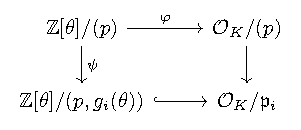
\includegraphics{lectures/4/pictures/cd_1.pdf}
 		 \end{center}

 		 Достаточно проверить, что $\Ker{\varphi} = 0$. Дейстивтельно, пусть $\overline{\alpha} \in \Ker{\varphi}$, тогда $\psi(\overline{\alpha}) = 0$, а значит, $\alpha \in (p, g_{i}(\theta)) \ \forall i$, из чего следует, что 
 		 \[
 		 	\alpha^k \in \prod_{i} (p, g_{i}(\theta)) \in p\Z[\theta] \implies \overline{\alpha}^k = \overline{0} \text{ в } \Z[\theta]/(p),
 		 \]
 		 то есть мы нашли нильпотентный элемент. С другой стороны, 
 		 \[
 		 	\Z[\theta]/(p) \cong \F_{p}[t]/\lr*{\overline{f}} \cong \bigoplus \F_{p}[t]/(\overline{g_i}), 
 		 \]
 		 а то, что написано справа~--- прямое произведение полей. Значит, $\overline{\alpha} = 0$  и ядро тривиально. 
 	\end{proof}

 	\noindent\bf{Ветвление при круговом расширении}

 	Оказывается, теорема Куммера~\ref{Kummer_theorem} позволяет полностью исследовать ветвление при круговом расширении. 

 	Пусть $p$~--- простое число, $K = \Q(\zeta_m)$ и $m \notdivby p$. Как мы знаем, минимальный многочлен $\zeta_m$~--- это круговой многочлен $\Phi_m$. Ясно, что 
 	\[
 		x^m - 1 \divby \Phi_m,
 	\]
 	так как $\Phi_m$~--- минимальный. С другой стороны, многочлен $\overline{x^m - 1}$ имеет $m$ попарно различных корней в $\F_{p}^{alg}$, так как он взаимнопрост со своей производной:
 	\[
 		(x^m - 1, (x^m - 1)') = (x^m - 1, m x^{m - 1}) = 1.
 	\]
 	Но тогда, так как $x^m - 1 \divby \Phi_m$,
 	\[
 		\overline{\Phi_m} = \overline{g_1} \cdot \ldots \overline{g_n},
 	\]
 	где $\overline{g_i}$~--- попарно различные и неприводимые. Тогда по теореме~\ref{Criterion_for_Kummer} $p \not \ \mid \ind(\zeta_m)$, то есть мы можем применить теорему Куммера~\ref{Kummer_theorem}:
 	\[
 	 	p\cO_{K} = \fp_{1} \cdot \ldots \fp_{k}, \quad \fp_{i} = (p, g_i(\zeta_m)). 
 	 \] 

 	 С другой стороны, так как $\Q(\zeta_m)/\Q$~--- расширение Галуа, все степени инерции равны. Значит, достаточно вычислить хотя бы одну. 

 	 \begin{statement} 
 	 	Степени инерции $f$ идеалов $\fp_i$~--- это минимальные такие $f$, что $(p^{f} - 1) \divby m$. 
 	 \end{statement}
 	 \begin{proof}
 	 	Корни многочлена $\overline{x^m - 1}$  образуют циклическую группу, так как это подгруппа в мультипликативной группе конечного расширения $\F_{p}$. Пусть $\theta$~--- образующая этой группы, $\theta \in \F_{p}^{alg}$. 

 	 	\[
 	 		x^m - 1 = \Phi_m(x) \cdot \prod_{k \mid m, k \neq m} \Phi_k(x) \implies \overline{x^m - 1} = \overline{\Phi_m(x)} \cdot \prod_{k \mid m, k \neq m} \overline{\Phi_k(x)}. 
 	 	\]
 	 	Пусть $\Phi_k(\theta) = 0$, тогда так как $x^k - 1 \divby \Phi_k$, $\theta^k - 1 = 0$, откуда $k \divby m$ (так как $\theta$~--- образующая циклической группы из $m$ элементов). Значит, $\overline{\Phi_m} = 0$. 

 	 	Не умаляя общности, пусть $\overline{g_{1}}(\theta) = 0$. Тогда 
 	 	\[
 	 		\{ 1, \theta, \ldots, \theta^{m - 1} \} = \langle \theta \rangle \le \lr*{\F_{p}[x]/(g_1)}^{*}.
 	 	\]
 	 	Тогда, если $\deg{g_1} = f_1$, мы имеем 
 	 	\[
 	 		\left\lvert \lr*{\F_{p}[x]/(g_1)}^{*} \right\rvert = p^{f_1} - 1, \quad \langle \theta \rangle \le lr*{\F_{p}[x]/(g_1)}^{*} \implies p^{f_1} - 1 \divby m,
 	 	\]
 	 	откуда $f_1 \ge f$.  Теперь докажем, что $f_1 \le f$. Действительно, 
 	 	\[
 	 		\begin{cases} \theta^m = 1 \\ m \mid p^{f} - 1 \end{cases} \implies \theta^{p^{f} - 1} = 1 \implies \theta^{p^f} = \theta.
 	 	\]
 	 	Значит, $\theta \in \F_{p^{f}} \implies \F_{p}[x]/(g_1) = \F_{p}[\theta] \le \F_{p^{f}}$, откуда $p^{f} \divby p^{f_1} \implies f_1 \le f$.    
 	 \end{proof}

 	

 		\begin{homework}
 			Задачи:
 			\begin{enumerate}
 				\item Рассмотрим кубическое расщирение $K = \Q(\sqrt[3]{15}) = \Q(\rho)$. 

 				0) Посчитать кольцо $\cO_{K}$.

 				а) Вычислить $\Nm(\rho), \ \Nm(\rho - 1), \ \Nm(\rho + 1), \Nm(\rho - 3)$.

 				б) Докажите, что над простым числом 3 лежит ровно один простой идеал $\rho_3$.

 				в) Докажите, что $\rho_3$~--- главный. Найдите его образующую с помощью разложений $(\rho - 3)$ и $(\rho + 3)$.

 				г) Докажите, что $\frac{9(\rho + 1)^3}{(\rho  - 3)^6}  \in \cO_{K}^{*}$. 

 				\item Вычислить $\cO_{K},$ где $K = \Q(\sqrt{p_1}, \ldots, \sqrt{p_k})$, если $p_i$~--- простые и $p_i \equiv 1 \pmod{4}$.
 				\item  Доказать, что $\upsilon_{\fp}(\cD) \ge e - 1$, где $ e = e(\fp)$~--- индекс ветвления. 

 			\end{enumerate}
 		\end{homework}

 		
 	

    % лекция 9: Первый случай Большой теоремы Ферма. Теорема Софи-Жермен, 
    	
	\subsection{Первый случай Last Fermat's theorem}

	Мы можем полагать, что показатель $n$~--- простое число, а также рассматривать уравнение в виде 
	\begin{equation}
		x^p + y^p + z^p = 0, \quad (x, y = z) = 1. \label{1_st_Last_Fermat's_Theorem}
	\end{equation}
	

	\begin{theorem}[Первый случай Большой теоремы Ферма]
		Уравнение~\ref{1_st_Last_Fermat's_Theorem} не имеет целых решений, если $p \not \mid xyz$.
	\end{theorem}

	\begin{theorem}[Софи Жермен] 
		Если простое число $p$ таково, что $2p + 1 = q$~--- простое число, то имеет место первый случай Большой теоремы Ферма. 
	\end{theorem}
	\begin{proof}
		Перепишем уравнение в виде 
		\[ 
			y^p + z^p = (-x)^p \Leftrightarrow (y + z)(y^{p - 1} + y^{p - 2}z + \ldots + z^{p - 1}) = (-x)^{p}.
		\]

		Покажем, что $(y + z, y^{p - 1} + y^{p - 2}z + \ldots + z^{p - 1}) = 1$. Пусть $r$~--- простое ($r \neq p$) и такое, что $r \mid y + z, \ r \mid y^{p - 1} + y^{p - 2}z + \ldots + z^{p - 1}$. Тогда 
		\[
			y \equiv -z \pmod{r}, \quad py^{p - 1} \equiv 0 \pmod{r} \implies py^{p - 1}\equiv 0 \pmod{r},
		\]
		что противоречит взаимной простоте. Тогда мы имеем 
		\[
			\begin{cases} 
				y + z = A^p \\
				y^{p - 1} + y^{p - 2}z + \ldots + z^{p - 1} = T^p
			\end{cases}
		\]

		Так как наше условие симметрично относительно переменных, $x + y = B^p, \ x + z = C^p$, откуда 
		\begin{equation}
				x^{\frac{q - 1}{2}} + y^{\frac{q - 1}{2}} + z^{\frac{q - 1}{2}} = 0. \label{ferm_2}
		\end{equation}

		Заметим, что если $q \not \mid x$,  то по малой теореме Ферма:
		\[
				x^{q - 1} \equiv 1 \pmod{q} \implies x^{\frac{q - 1}{2}} \equiv \pm 1 \pmod{q}.
			\]	
		Ясно, что отсюдо следует протвиоерчие~\eqref{ferm_2}. Значит, $q \mid xyz$.  Не умаляя общности, $q \ \mid x$. Тогда 
		\[
			2x = B^p + C^p - A^p = B^{\frac{q - 1}{2}} + C^{\frac{q - 1}{2}} - A^{\frac{q - 1}{2}} \ \vdots \ q.
		\]

		Заметим, что $q \not \ \mid B, \ q \not\  \mid C$, значит $q \not \ \mid BC \implies q \mid A$. Тогда $q \mid y + z$.  

		Заметим, что  $T^p \equiv py^{p - 1} \pmod{q}$. Так как $(A, T) = 1$, $q \not\  \mid T$. Тогда $T^{\frac{q - 1}{2}} \equiv py^{p - 1} \pmod{q}$, тогда по малой теореме Ферма $\pm 1 = p y^{p - 1} \pmod{q}$.  Так как $q \mid x$,  $B^p = x + y \equiv y \pmod{q}$. Значит, 
		\[
			y \equiv B^{\frac{q - 1}{2}} \equiv \pm 1 \pmod {1}, \text{ так как } q \not \ \mid B.
		\]

		Знчит, $\pm 1 \equiv \pm p \pmod{q}$, а этого быть не может, так как $q = 2p + 1$.

	\end{proof}

	\begin{homework}
		Получите элементарное доказательство случая $p = 5$ в первом случае большой теоремы Ферма. 
	\end{homework}

	Как мы знаем, если мы рассматриваем расширение $K = \Q(\zeta_m)$ над $\Q$ и простое число $q \not \mid m$, число $q$ не равзетвлено. 

	В частности для $m = p$~--- простого, $q \neq p \implies q$ неразветвлено в $\Q(\zeta_p)$.

	\begin{statement}\label{stm:11} 
		Простое число $p$ полностью разветвлено в $\Q(\zeta_{p})$.
	\end{statement}
	\begin{proof}
		\[
	 	x^p - 1 = (x - 1)(x - \zeta)(x - \zeta^2)\ldots(x - \zeta^{p - 1})
	 \] 
	 \[
	 	x^{p - 1} + \ldots + x + 1 = (x - \zeta)(x - \zeta^2)\ldots(x - \zeta^{p - 1})
 	 \]

 	 Подставим $x = 1$ и от числового равенства перейдём к равенству идеалов: 
 	 \[
 	 	p = ((1 - \zeta))((1 - \zeta^2))\ldots((1 - \zeta^{p - 1})),
 	 \]
 	 отсюда, так как $\zeta = \lr*{\zeta^i}^j$, все идеалы в правой части совпадают, а значит, $(p) = ((1 - \zeta))^{p - 1}$, а это означает, что $p$ полностью разветвлено. Действительно, пусть 
 	 \[
 	 	1 - \zeta = \fp_{1}\fp_{2} \ldots \fp_{k} \implies (1 - \zeta)^{p - 1} = \fp_{1}^{p - 1}\fp_{2}^{p - 1} \ldots \fp_{k}^{p - 1},
 	 \]
 	 из чего следует, что степень ветвления каждого $\fp_i$ хотя бы $p - 1$. С другой стороны, $\sum e_j f_j = p - 1$, то есть $(p) = \fp^{p - 1}$.
	\end{proof}

	\begin{lemma} 
		Пусть $p$~--- простое число, не равное двум. Множество корней из единицы\footnote{не обязательно степени $p$} в поле $\Q(\zeta_{p})$ равно $\{ \pm \zeta_{p}^{i} \}.$
	\end{lemma}
	\begin{proof}
		Возьмем $\zeta_n \in \Q(\zeta_{p})$. Предположим, что $n \equiv 0 \pmod{4}$. Тогда $i = \zeta_{4} \in \Q(\zeta_{p})$. Заметим, что $2i = (1 + i)^2$ а значит, $(2) = ((1 + i))^2$. Значит, двойка разветвлена в $\Q(\zeta_{p})$ (а это противоречит предыдущему утверждению). Значит $n \not\equiv 0 \pmod{4}$. 

		Теперь рассмотрим случай  $n = 2n_{0}$, $n \equiv 1 \pmod{2}$. Тогда $\{\zeta^{i}_{n}\} = \{ \pm \zeta_{n_0}^{i}\}$ и нам достаточно рассматривать $n_0$. Предположим, что существует простое $p' \neq p \colon p \ \mid \ n_0$. Тогда $\zeta_{p'} \in \Q(\zeta_{p})$, но $\zeta_{p'} \in \Q(\zeta_{p'})$, а так как $p' \mid n_0$, $\Q(\zeta_{p'}) \subset \Q(\zeta_{n_0}) \subset \Q(\zeta_{p})$. Простое число $p'$ будет полностью разветвлено в $\Q(\zeta_{p'})$, а значит, оно будет полностью разветвлено и $\Q(\zeta_{p})$, но это противоречит утверждению~\ref{stm:11}.
		

		Значит, $n_0 = p^a$, а тогда $\zeta_{p^{a}} \in \Q(\zeta_{p})$. Но это приводит нас к тому, что $n_0 = p$, ведь 
		\[
			[\Q(\zeta_{p^{a}}) : \Q] = p^{a} - p^{a - 1} \le [\Q(\zeta_{p}) : \Q] = p - 1 \implies a - 1 \implies n_0 = p 
		\]
	\end{proof}

	\begin{lemma}\label{lemma:14}
		Пусть $K/\Q$~--- конечное расширение, $\sigma_i \colon K \to \Q^{alg}$~--- все вложения ($1 \le i \le n$, $n = [K : \Q]$). Предположим, что $\alpha \in \cO_{K}$ и $\forall i \ |\sigma_{i}\alpha| = 1$. Тогда $\alpha$ является корнем из единицы какой-то степени. \footnote{Обратное утверждение очевидно.}
 	\end{lemma}
 	\begin{proof}
 		Выпишем многочлен с целыми коэффициентами, корнем которого является $\alpha$:
 		\[
 			\prod_{i} (x - \sigma_{i} \alpha) \in \Z[x].
 		\]
 		В силу предположения теоремы, его коэффиценты ограничены, так как они являются симметрическими функциями от $\sigma_{i}\alpha$. Заметим теперь, что из условия следует, что $|\sigma_{i}(\alpha^k)| \le 1$, а значит, для $\alpha^k$ мы также получим многочлен с ограниченными коэффициентами. Заметим, что $k$~--- произвольное натуральное, а значит, мы получаем бесконечное число $\alpha^k$, которые являются корнями коненого набора многочленов над $\Z$ (так как коэффициенты  каждого мы можем ограничить одной и той же константой).  Значит, $\exists m, n \colon \alpha^m = \alpha^n$, что и даёт нам, что $\alpha$~--- корень из 1. 
 	\end{proof}

 	\begin{lemma} 
 		Пусть $u \in \cO_{K}^{*} = \Z[\zeta_{p}]$ для $K = \Q(\zeta_{p})$. Тогда $\exists s \colon u \zeta^{s} \in \R$.

 		\begin{proof}
 			Рассомтрим $v = u / \overline{u}$ и возьмем $\rho \in \Gal\lr*{\Q(\zeta_{p})/\Q} \cong (\Z/p\Z)^{*}$. Тогда по лемме~\ref{lemma:14}:
 			\[
 				\rho(v) = \frac{\rho(u)}{\rho(\overline{u})}  = \frac{\rho(u)}{\overline{\rho(u)}}	 \implies |\rho(v)| = 1 \implies v = \pm \zeta_{p}^{n}.
		 	\] 	

		 	Рассмотрим $\lambda = 1 - \zeta$, тогда 
		 	\[
		 		\rho(\zeta) \equiv \zeta^k \equiv \zeta \pmod{\lambda} \implies \rho(\zeta^i) \equiv \zeta^i \pmod{\lambda},
		 	\]
		 	а так как $\cO_{K} = \Z[\zeta_{p}]$, мы имеем такое сравнение для всеё элементов $\cO_{K}$. В частности, из этого следует, что $\rho(u) \equiv u \pmod{\lambda}$. В частности, мы можем положить $\rho(\cdot) = \overline{\cdot}$ и отсюда получить, что $\overline{u} \equiv u \pmod{\lambda}$. Из этого следует, что 
		 	\begin{multline*}
		 		\pm \zeta^{n}_{p} \overline{u} \equiv u \equiv \overline{u} \pmod{\lambda}, \text{пусть } -\zeta^{n}_{p}u \equiv u \pmod{\lambda}, \\ -\zeta^{n}_{p}\overline{u} \equiv \overline{u} \pmod{\lambda} \implies -u \equiv u \pmod{\lambda} \implies 2u \equiv 0 \pmod{\lambda},
		 	\end{multline*}
		 	но если $2u \ \vdots \  (1 - \zeta)$, то так как $u$ обратим, $2 \ \vdots \ (1 - \zeta)$.  Но, если $2 \in (1 - \zeta)$, то $2^{p - 1} \in ((1 - \zeta))^{p - 1} = (p)$. Значит, знак минус невозможен и реализуется случай 
		 	\[
		 		\zeta^n_{p} \overline{u} \equiv \overline{u} \equiv u \pmod{\lambda}. 
		 	\]
		 	Так как $u - v \overline{u}$, $u = \zeta^{n}_{p} \overline{u}$, тогда $u \zeta_{p}^{s} = \zeta_{p}^{n + s}\overline{u}$. Найдём такое $s$, что $\overline{\zeta_{p}^{n + s} \overline{u}} = u$. То есть, такое $s$, что $\overline{\zeta^{n + s}} = \zeta^{s} \implies 2s + n \equiv 0 \pmod{p}$, что вполне возможно реализовать. 
 		\end{proof}
 	\end{lemma}

 	\begin{lemma}\label{lemma:15}
 		Пусть $x^p + y^p = z^p, \ p \not \ \mid xyz, \ (x, y, z) = 1$, разложим левую часть в линейные множители:
 	\[
 		(x + y)(x + \zeta y)\ldots(x + \zeta^{p - 1}y)
 	\]
 	Тогда  эти сомножители взаимнопросты. 	
 	\end{lemma}
 	

 	\begin{proof}
 		Предположим противное, тогда $x + \zeta^i y, \ x + \zeta^{j} y \in \fq$ для некоторых $i, j$. Тогда $\zeta^i(1 - \zeta^{j - i}) y \in \fq$, но $((1 - \zeta^{j - i}))^{p - 1} = (p)$ и если $\fq \neq (1 - \zeta)$, мы получаем, что $y \in \fq$, но тогда и $x \in \fq$, а это противоречит взаимной простоте $x$ и $y$. Если же $\fq = (1 - \zeta)$, мы получаем, что $x + y = x + \zeta^{i}y + (y - \zeta^{i})y \in \fq$, откуда следует, что $z \in \fq$, а значит, $z^{p - 1} \ \vdots p$, а этого не может быть по предположению. 
 	\end{proof}


 	\begin{theorem} 
 		Пусть $p \not \ \mid |\Cl(\Q_{\zeta_{p}})|$\footnote{такие простые числа называются регуярными}. Тогда имеет место первый случай Великой теоремы Ферма.  
 	\end{theorem}
 	\begin{proof}
 		Пусть $x^p + y^p = z^p$, разложим левую часть на множители: 
 		\[
 			\prod_{i = 0}^{p - 1} (x + \zeta^{i}y) = z^p,
 		\]
 		а так как все сомножители в левой части равенства взаимнопросты по лемме~\ref{lemma:15}. Значит, все они являются $p$-ми степенями, в частности для $i = 1$. То есть 
 		\[
 			(x + \zeta y) = I^{p},
 		\]
 		значит $I$ находится в $p$-кручении $\Cl(\Q_{\zeta_{p}})$, но так как $p$ не делит порядок группы классов, оно тривиально, значит  $I$--- главный, то есть  $I = (\alpha)$.  Значит,

 		\[
 			(x + \zeta y) = (\alpha^p) \implies x + \zeta y = \varepsilon \alpha^p, \ \varepsilon \in \Z[\zeta]^{*}, \ \varepsilon = \zeta^s u \implies x + \zeta y = \zeta^s u \alpha^p.
 		\]

 		С другой стороны, $\alpha = a_0 + a_1 \zeta_{p} + \ldots + a_{p - 2}\zeta^{p - 2}$. Тогда 
 		\[
 		 	\alpha^p \equiv \underbrace{a_0^p + a_1^p + \ldots + a_{p - 2}^{p}}_{\eqdef n} \pmod{p}.
 		 \] 

 		 Тогда $x + \zeta y \equiv \zeta^s u n \pmod{p}$. Переходя в этом сравнении к сопряженным, мы получаем 
 		 \[
 		 	x + \zeta y \equiv \zeta^s u n \pmod{p}, \quad x + \zeta^{-1}y \equiv \zeta^{-s} \overline{u} n = \zeta^{-s} u n \pmod{p}, \text{ так как } u \in \R.
 		 \]

 		 Отсюда мы получаем, что $\zeta^{-s}(x + \zeta y) \equiv \zeta^{s} (x + \zeta^{-1}y)\pmod{p}$. Значит, $x + \zeta y - \zeta^{2s} x - \zeta^{2s - 1}y \in p\Z[\zeta]$. Теперь рассмотрим несколько случаев: 

 		 \begin{enumerate}
 		 	\item Элементы $S = \{ 1, \zeta, \zeta^{2s}, \zeta^{2s - 1}\}$~--- попарно различны. 
 		 	\begin{enumerate}
 		 		\item Если $\zeta^{p - 1} \notin S$, то $p \mid x, p \mid y$. 

 		 		\item Если $\zeta^{p - 1} \in S$, то $p = 2s - 1$ и тогда $s \ \vdots p $, а значит $(\zeta - \zeta^{-1})y \in p\Z[\zeta]$ откуда следует, что $p \mid 1 - \zeta^2$, что даёт нам противоречие. 

 		 		\item Если $\zeta^{p - 1} = -(1 + \zeta + \ldots + \zeta^{p - 2})= \zeta^{2s}$, то $x + \zeta y - \zeta^{-1}x - \zeta^{-2}y \in \Z[\zeta]$, а тогда 
 		 		\[
 		 			x + \zeta y + ((1 + \zeta + \ldots + \zeta^{p - 2}))x - \zeta^{p - 2}y \ \vdots \ p \implies x + y \ \vdots \  p \implies z \ \vdots \ p,
 		 		\]
 		 		что даёт нам противоречие. 
 		 	\end{enumerate}

 		 	\item Некоторые из этих степеней совпадают. 
 		 		\begin{enumerate}
 		 			\item $\zeta^{2s} = 1$. В этом случае $(\zeta - \zeta^{-1})y \ \vdots \ p$,  а мы уже видели, что это невозможно. 

 		 			\item $\zeta^{2s - 1} = 1$.  В этом случае $x - y + \zeta y - \zeta x \ \vdots \ p \implies (x - y)(1 - \zeta) \ \vdots \ p \implies x - y \ \vdots \ p$, то есть $x \equiv y \pmod{p}$. Исходное уравнение мы можем записать в виде 
 		 			\[
 		 				z^p + (-y)^p = x^p,
 		 			\]
 		 			и рассуждая аналогично, мы можем получить, что $z \equiv - y \pmod{p}$. Тогда 
 		 			\[
 		 				x^p + x^p \equiv (-x)^{p} \pmod{p} \implies 3x^{-} \equiv 0 \pmod{p}.
 		 			\]
 		 			Значит, либо $p = 3$ (в этом случае мы полностью разобрали вообще всю теорему Ферма), либо $p \mid x$, что даёт нам противоречие. 
 		 			

 		 			\item $\zeta = \zeta^{2s - 2}$. Тогда $x - \zeta^2 x \ \vdots \ p$, откуда следует, что $1 - \zeta^2 \ \vdots \ p$, а это, как мы уже видели, противоречие. 
 		 		\end{enumerate}
 		 \end{enumerate}

 		 Дадим теперь хороший критерий для проверки условия теоремы. Этот критерий мы дадим без доказательства, так как он доказывается методами аналитической теории чисел. 

 		 Как мы помним, числа Бернулли можно начинать через экспоненциальную производящую функцию: 
 		 \[
 		 	\frac{t}{e^t - 1} = \sum_{m = 0}^{\infty} B_{m} \frac{t^m}{m!}.
 		 \]
 		 Подставим $-t$:
 		 \[
 		 	\frac{-t}{\frac{1}{e^{t}} - 1} = \frac{t e^{t}}{e^{t} - 1} = \frac{t(e^t - 1) + t}{e^t - 1} = t + \frac{t}{e^t - 1}.
 		 \]

 		 Отсюда мы можем понять, чему равны коэффициенты: 
 		 \[
 		 	m > 1, \ m \equiv_{2} 1 \implies B_m = -B_m \implies B_m = 0.
 		 \]
 		 \[
 		 	-(n + 1)B_n = \binom{n + 1}{n - 1} B_{n - 1} + \ldots + \binom{n + 1}{k}B_{k} + \ldots + \binom{n + 1}{1} B_{1} + 1. 
 		 \]
 		 Так как все нечётные коэффициенты равны нулю, авторы часто используют обозначение $B_n$ для $2n$-го числа Бернулли. Например, известно, что 
 		 \[
 		 	B_{n} = -n \zeta(1 - n), n > 1.
 		 \]

 		 \begin{theorem} 
 		 	Простое число $p$~--- регулярно тогда и только тогда, когда числители всех чисел Бернулли $B_{2}, B_{3}, \ldots, B_{p - 3}$ не делятся на $p$.
 		 \end{theorem}

 		 Из этого рекуррентного соотношения следует, что знаменатели $B_n$ не делятся на $p$ при $n \le p - 3$ , так как 
 		 \[
 		 	\upsilon_{p}((n + 1)B_n) \ge 0 \implies \upsilon_{p}(B_n) \ge 0.
 		 \]

 		 \begin{example}
 		 	Например, таким образом нетрудно показать, что число 7 является регулярным. 
 		 \end{example}

 	\end{proof}

 	Теперь, немного отвлечёмся и приведём алгоритм построение целого базиса.

 	\subsection{Алгоритм построения целого базиса}

 	Итак, для $d = \disc(1, \alpha, \alpha^2, \ldots, \alpha^{n - 1})$ мы наем, что 
 	$d \cO_{k} \subset \Z[\alpha] \subset \cO_{k}$, откуда 
 	\[
 		\Z[\alpha] \subset \cO_{K} \subset d^{-1}\Z[\alpha].
 	\]

 	Тогда, как мы помним, $\bigcup (\omega_i + \Z[\alpha]) = d^{-1}\Z[\alpha]$, причем, каждый класс, либо вообще не содержит целых алгебраических чисел, либо целиком из них состоит. То есть, отсюда мы имеем 
 	\[
 		\cO_{K} = \bigcup_{i \in I} (\omega_{i} + \Z[\alpha]),
 	\]
 	откуда следует, что $\cO_{K}$ порождена $\omega_{i}$ и $\alpha^s$ при $0 \le s \le n - 1$. Значит, $d \cO_{K}$ будет порождена  $d\omega_{i}$ и $d \alpha^s$. С другой стороны, $d\cO_{K}$~--- подгруппа свободной абелевой группы $\Z[\alpha]$, значит мы попадаем в контекст \hyperlink{smith_normal_form}{нормальной формы Смита}.

 	\begin{homework}

 	\begin{enumerate}
 		\item \begin{theorem}[Штикельберг] 
 			Дискриминант конечного расширения $K/\Q$ сравним с нулём или единицей по модулю 4. 
 		\end{theorem}
 		\emph{Hint:} Можно действовать так: $\disc(K) = \lr*{\det(\sigma_i)}^2$, и раскрывая определитель, мы получаем $\det(\sigma_{j}\omega_{j}) = P - N$, где $P$~--- сумма произведений со знаком +, а $N$~--- сумма произведений со знаком минус. Тогда $\disc(K) = (P - N)^2 = (P + N)^2 - 4 PN$. Значит, достаточно показать, что числа $P + N$ и $PN$~--- целые.  \emph{Hint:} Целое число~--- это рациональное число, которое еще и целое алгебраическое. 
 		\item
 	\end{enumerate}
 		
 	\end{homework}





	
    % лекция 10: Решетки, теорема Минковского, оценка на порядок группы классов идеалов 
    
\subsection{Геометрия чисел}

	Рассмотрим евклидово пространство $\R^n$ и выберем в нём набор из $k$ линейно независимых векторов $e_1, \ldots, e_k$ и рассмотрим порожденную ими свободную абелеву группу:
	\[ L = \bigoplus_{i = 1}^{k} \Z e_i \]
	Тогда $L$ мы будем называть \emph{решёткой}, натянутой на вектора $e_1, \ldots, e_k$. В случае $k = n$ решётка $L$ называется \emph{полной}. 

	\begin{example}
		Картинка для $L \subset \R^2$.
	\end{example}

	\begin{statement} 
		В любом ограниченном подмножестве $\R^n$ лежит конечное число точек решётки. 
	\end{statement}

	\begin{proof}
		Очевидно.
	\end{proof}

	Оказывается, верно и обратное утверждение. 

	\begin{statement} 
		Пусть $A \le \R^n$~--- подгруппа (как абелевой группы), причем такая, что в любом ограниченном подмножестве $\R^n$ лежит конечное число элементов из $A$. Тогда $A$~--- решётка. 
	\end{statement}

	\begin{proof}
		Рассмотрим подпространство $\Span(A)$ в $\R^n$. Оно прождено некоторым линейно независимым набором векторов: 
		\[
			\Span(A) = \langle e_1, \ldots, e_m \rangle, \ e_i \in A \text{~--- линейно независимы}.
		\]
		Рассмотрим свободную абелеву группу, порожденную этими векторами: 
		\[
			A_0  = \Z e_1 + \ldots + \Z e_m.
		\]
		Покажем, что $A/A_0$ конечна. Расммотрим \emph{фундаментальную область}
		\[
			\Delta = \left\{  \sum_{i = 1}^{m} x_i e_i \ \bigg\vert \ 0 \le x_i < 1 \right\}
		\]
		Ясно, что $\forall a \in A \ \exists a_0 \in A_0\colon a - a_0 \in \Delta$. Но так как $\Delta$ ограничено, в нём может лежать только конечное число элементов решётки, значит количество значений, которые может принимать $a - a_0$ конечно и $A/A_0$ конечна. 

		Значит, $\exists s \in \Z \setminus \{ 0 \}\colon sA \subset A_0$.  Тогда $A \subset \frac{1}{s}A_0 = \Z \frac{e_1}{s} \oplus \Z \frac{e_2}{s} \oplus \ldots \oplus \Z \frac{e_m}{s} = A'$. Значит, $A_0 \subset A \subset A'$ и $A_0$ и $A'$~--- свободные абелевы группы одного и того же ранга. Значит и $A$~--- свободная абелева группа, 
		\[
		 	A = \Z u_1 \oplus \Z u_2 \oplus \ldots \oplus \Z u_m.
		 \] 

		 Кроме того, $\dim\langle u_1, \ldots, u_m \rangle \ge m$, откуда следует, что $u_1, \ldots, u_m$~--- линейно незавимы над $\R$, откуда $A$~--- решётка. 
	\end{proof}

	Это предложение даёт хороший критерий для проверки, является ли какое-то подпространство решёткой. 

	\begin{definition} 
		Если $L \le \R^n$~--- решётка с порождающим набором $e_1, \ldots, e_m$, то множество 
		\[
			\Delta = \left\{  \sum_{i = 1}^{m} x_i e_i \ \bigg\vert \ 0 \le x_i < 1 \right\}
		\]
		называют \emph{основным параллелипипедом} решётки или же \emph{фундаментальной областью} решётки. 
	\end{definition}

	Если $e_1, \ldots, e_m$~--- порождающий набор решётки $L$, то $\R^m = \Span\{ e_1, \ldots, e_m \}$ и тогда 
	мы можем вычислить объем фундаментальной области, как
	\[
		\Vol(\Delta) = \det\left\lvert (a_{i j})\right\rvert,  
	\]
	где $e_i = (a_{i 1}, a_{i 2}, \ldots, a_{i n})$.

	\begin{lemma}\label{lattice_prop_volume}
		Пусть $T$~--- ограниченное измеримое множество в $\R^m$, $L$~--- решётка ранга $m$ в $\R^m$, $\Delta$~--- её фундаментальная область. Предположим, что $\forall \ell_1, \ell_2 \in L $ множества $T + \ell_1$ и $T + \ell_2$ не пересекаются.  Тогда 
		\[
			\Vol(T) \le \Vol(\Delta).
		\]
	\end{lemma}
	\begin{proof}
		В самом деле, так как множества  $T + \ell$ дизъюнктны, 
		\[
			\Vol(\Delta) \ge \sum_{\ell \in L} \Vol(\Delta \cap T_{\ell}) = \sum_{\ell \in L} \Vol(\Delta_{-\ell} \cap T) = \Vol\lr*{\ \bigcup_{\ell \in L} \Delta_{\ell} \cap T} = \Vol(\R^m \cap T) = \Vol(T).
		\]
	\end{proof}

	\begin{lemma}[Г. Минковский, О выпуклом теле]\label{Mink_theorem}
		Пусть $T$~--- ограниченное выпуклое центрально-симметричное (относительно нуля) измеримое подмножество $\R^n$, $L$~--- решётка ранга $n$ в $\R^n$, $\Delta$~--- её фундаментальная область. Предположим, что выполнена следующая оценка на объемы:
		\[
			\Vol(T) > 2^n \Vol(\Delta).
		\]
		Тогда $\exists 0 \neq \ell \in L\colon \ell \in T$. Кроме того, если $T$ компактно, то это будет верно и в случае нестрогого неравенства $\Vol(T) \ge 2^n \Vol(\Delta)$.
	\end{lemma}
	\begin{proof}
		Рассмотрим тело $\frac{1}{2}T$, тогда $\Vol\lr*{\frac{1}{2}T} = \frac{1}{2^n} \Vol(T) > \Vol(\Delta)$. Тогда по предыдущей лемме~\ref{lattice_prop_volume}  $\exists \ell_1, \ell_2 \in L\colon \frac{1}{2}T_{\ell_1} \cap \frac{1}{2}T_{\ell_{2}} \neq \varnothing$. Это означает, что
		 \[ \exists t_1, t_2 \in T\colon \frac{x_1}{2} + \ell_1 = \frac{x_2}{2} + \ell_2 \implies 0 \neq \frac{x_1 - x_2}{2} = \ell_1 - \ell_2 \in L \cap T.\]

		 В последнем равенстве $\frac{x_1 - x_2}{2} \in T$ так как $T$~--- выпукло и центрально симметрично. 

		 Теперь докажем вторую часть теоремы. Рассмотрим $T_{\varepsilon} = (1 + \varepsilon)T$, для него неравенство уже будет строгим и по первой части теоремы мы получим $0\neq \ell \in L \cap T_{\varepsilon}$. Понятно, что если $\ell \in T$, всё доказано. Пусть теперь $\ell \in T_{\varepsilon} \setminus T$. Вообще говоря, в $T_{\varepsilon} \setminus T$  лежит лишь конечное число точек из $L$. Так как $T_{\varepsilon}$ замкнуто, мы можем уменьшить $\varepsilon$ так, чтоб все точки из $\ell$, лежащие в $T_{\varepsilon}\setminus T$ уже не лежали там. 
	\end{proof}

	\hypertarget{real_and_complex_inclusions}{}
	Рассмотрим теперь конечное расширение $K/\Q$, $[K : \Q] = n$. Тогда у нас есть $n$ вложений $\sigma_i \colon K \to \Q^{alg}$. Среди них есть \emph{вещественные} вложения, то есть такие, что $\Im(\sigma_i) \subset \R$. Остальные вложения  называют \emph{невещественными}. С каждым невещественным вложением $\sigma_i$ связано вложение $\overline{\sigma_i} \neq \sigma_i$. Пронумеруем наши вложения следующим образом: $\sigma_1, \ldots, \sigma_s$~--- вещественные вложения, $\sigma_{s + 1}, \overline{\sigma_{s + 1}}, \sigma_{s + 2}, \overline{\sigma_{s + 2}}, \ldots, \sigma_{s + t}, \overline{\sigma_{s + t}}$~--- невещественные вложения. Так как количество вложений равно степени расширения, $s + 2t = n$.

	Рассмотрим отображение $\varphi\colon K \to \R^n$, которое действует так:
	\[
		\alpha \in K, \ \alpha \mapsto (\sigma_1(\alpha), \sigma_2(\alpha), \ldots, \sigma_s(\alpha), \Re(\sigma_{s + 1}(\alpha)), \Im(\sigma_{s + 1}(\alpha)),  \ldots, \Re(\sigma_{s + t}(\alpha)), \Im(\sigma_{s + t}(\alpha))) \in \R^n.
	\]
	\hypertarget{phi_from_this}{}

	Пусть $I$~--- ненулевой идеал в $\cO_{K}$. Возьмём его базис как абелевой группы~--- $\alpha_1, \ldots, \alpha_n$. Тогда $\varphi(I)$~--- решётка в $\R^n$ с базисом $\varphi(\alpha_1), \ldots, \varphi(\alpha_n)$. Нужно проверить равзе что линейную независимость. 

	Пусть $\sigma_{s + 1}(\alpha) = a + bi$, будем делать слудеющие преобразование: $(a, b) \mapsto (a, bi) \mapsto (a + bi, bi) \mapsto (a + bi, 2bi) \mapsto (a + bi, -a + bi) \mapsto (a + bi, a - bi)$. Посмотрим, что будет происходить с определителем при проделывании этих операций. Нетрудно проследить, что по итогу определитель умножится на $-2i$. В итоге мы получим, что 
	\[
		\det\lr*{\begin{pmatrix} \varphi(\alpha_1) \\ \varphi(\alpha_2) \\ \vdots \\ \varphi(\alpha_n) \end{pmatrix}} = \frac{1}{(2i)^t} \det{\begin{pmatrix} \sigma_{1}(\alpha_1) & \ldots& \sigma_{s + 1}(\alpha) & \sigma_{s + 1}(\alpha_1) & \ldots \overline{\sigma_{s + t}(\alpha)} \\ \vdots & \vdots & \vdots & \vdots & \vdots & \vdots\end{pmatrix}} = \pm \sqrt{\disc(\alpha_1, \ldots, \alpha_n)}.
	\]

	А теперь заметим, что 
	\[
		\Vol(\Delta) = \det(M)
 = \frac{1}{2^t} \sqrt{\disc(\alpha_1, \ldots, \alpha_n)} = \frac{1}{2^t} \sqrt{\disc(K) \cdot [\cO_{K} : I]^2} = \frac{1}{2^t} \Nm(I) \sqrt{\disc(K)}.	\]

 	Рассмотрим теперь для некоторого фиксированного $a > 0$.
 	\[
 		T = \{ (x_1, x_2, \ldots, x_{s}, y_{1}, z_{1}, \ldots, y_{t}, z_{t}), \ |x_1| + \ldots + |x_1| + 2\sqrt{y_1^2 + z_1^2} + \ldots + 2\sqrt{y_t^2 + z_t^2} \le a \}. 
 	\]

 	$T$~--- выпуклое, центрально-симметричное и $\Vol(T) = 2^s \lr*{\frac{\pi}{2}}^t \frac{a^n}{n!}$.
 	Пусть $I$~--- ненулевой идеал в $\cO_{K}$. Подберём $a$ так, что будет выполнено неравенство 
 	\begin{equation}
 		2^s \lr*{\frac{\pi}{2}}^t \frac{a^n}{n!} > 2^n \frac{\sqrt{\disc(K)}}{2^t} \Nm(I). \label{calculating_a}
 	\end{equation}

 	Тогда по лемме Минковского~\label{Mink_theorem} $\exists 0 \neq \alpha \in I\colon$
 	\[
 	 	|\sigma_1(\alpha)| + \ldots + |\sigma_{s}(\alpha)| + 2 |\sigma_{s + 1}(\alpha)| + \ldots +  2|\sigma_{s + t}(\alpha)| \le a.
 	 \] 
 	 Это неравенство мы можем переписать в виде: 
 	 \[
 	 	|\sigma_1(\alpha)| + \ldots + |\sigma_{s}(\alpha)| + |\sigma_{s + 1}(\alpha)| + |\overline{\sigma_{s + 1}}(\alpha)| + \ldots +  |\sigma_{s + t}(\alpha)| + |\overline{\sigma_{s + t}}(\alpha)| \le a.
 	 \]

 	  Тогда по неравенству о среднем мы имеем 
 	  \[
 	  	\left\lvert \sigma_{1}(\alpha) \cdot \ldots \cdot \sigma_{s}(\alpha)\overline{\sigma_{s + 1}(\alpha)} \cdot \ldots \cdot \sigma_{s + t}(\alpha) \overline{\sigma_{s + t}}(\alpha) \right\rvert \le \lr*{\frac{a}{n}}^n \Leftrightarrow \Nm(\alpha) \le \lr*{\frac{a}{n}}^n
 	  \]

 	  Заметим, что в неравенстве~\eqref{calculating_a} равенство будет достигаться при 
 	  \[
 	  	a^n = \frac{2^n \sqrt{\disc(K)} \Nm(I) n!}{2^t 2^s} \cdot \lr*{\frac{2}{\pi}}^t = \lr*{\frac{4}{\pi}}^{t} n! \Nm(\alpha) \sqrt{\disc{K}}.
 	  \]
 	  В этом случае будет выполняться неравенство
 	  \[
 	  		\Nm(\alpha) \le \lr*{\frac{a}{n}}^n = \lr*{\frac{4}{\pi}}^t \frac{n!}{n^n} \Nm(I) \sqrt{\disc{K}}.
 	  \]

 	  Подставим в этом неравенство, например, единичный идеал. Тогда мы получим неравенство 
 	  \[
 	  	1 \le \lr*{\frac{4}{\pi}}^t \frac{n!}{n^n} \sqrt{\disc{K}}.
 	  \]

 	  Например, из этого неравенства следует, что $\disc(K) \neq 1$ (в случае нетривиального расширения).  

 	  \begin{theorem} 
 	  	Пусть $K/\Q$~--- конечное расширение, $[K : \Q] = n > 1$. Тогда $\disc(K) \neq 1$. Кроме того, 
 	  	\[
 	  	 	\lim\limits_{n \to \infty} \disc(K) = \infty.
 	  	 \] 
 	  \end{theorem}

 	  Получим теперь при помощи новых методов некоторые результаты, связанные с группой классов идеалов числового поля. 

 	  Мы доказали, что для ненулевого идеала $I$ в $\cO_{K}$ существует $\alpha \in I\colon$
 	  \[
 	  		\Nm(\alpha) \le \lr*{\frac{4}{\pi}}^t \frac{n!}{n^n} \Nm(I) \sqrt{\disc{K}}.
 	  \]

 	  Возьмём класс $[I^{-1}] \in \Cl(K)$ и представим его идеалом $I \subset \cO_{K}$. С одной стороны, $\alpha I^{-1}$ представляет тот же класс в группе классов, а с другой стороны, 
 	  \[
 	  	\Nm(\underbrace{\alpha I^{-1}}_{\text{целый}}) = \Nm(\alpha) \Nm\lr*{I^{-1}} \le \lr*{\frac{4}{\pi}}^{t} \frac{n!}{n^n} \sqrt{|\disc(K)|}.
 	  \]

 	  Но, как мы уже замечали, существует лишь конечное число целых идеалов с ограниченной нормой. 

 	  \begin{example}
 	  	Рассмотрим $K = \Q\lr*{\sqrt[3]{6}}$. Посмотрим сначала на количество вложений. Нетрудно убедиться в том, что $n = 3, t = 1$. Сосчитаем теперь дискриминант $K$. Для этого покажем, что $\cO_{K} = \Z[\sqrt[3]{6}]$. Обозначим $\theta = \sqrt[3]{6}$ и посчитаем $[\cO_{K} : \Z[\theta]]$.
 	  Заметим, что минимальный многочлен $\theta$~--- это $x^3 - 6$, а минимальный многочлен $\theta^2$~--- это $x^2 - 36$, а тогда 

 	  \[
 	  	\disc(K) \cdot \lr*{\ind(\theta)}^2 = \disc(1, \theta, \theta^2) = \det\begin{pmatrix} \Tr(1) & \Tr(\theta) & \Tr(\theta^2) \\ \Tr(\theta) & \Tr(\theta^2) & \Tr(\theta^3) \\ \Tr(\theta^2) & \Tr(\theta^3) & \Tr(\theta^4) \end{pmatrix} = \det\begin{pmatrix} 3 & 0 & 0 \\ 0 & 0 & 18 \\ 0 & 18 & 0 \end{pmatrix} = - 2^{2} 3^{5}.
 	  \]

 	  Заметим, что многочлен $x^3 - 6$ является многочленом Эйзенштейна относительно и двойки и тройки, а значит, $\ind(\theta)$ не может делиться на $2$ и $3$, откуда $\ind(\theta) = 1$. Значит, $\disc(K) = -2^5 \cdot 3^5$. Подставим это в неравенство выше: 
 	  \[
 	  	\Nm(\underbrace{\alpha I^{-1}}_{\text{целый}}) = \Nm(\alpha) \Nm\lr*{I^{-1}} \le \lr*{\frac{4}{\pi}}^{t} \frac{n!}{n^n} \sqrt{|\disc(K)|} = \frac{4}{\pi} \cdot \frac{6}{27} \cdot \sqrt{2^5 \cdot 3^5} < \frac{16}{\sqrt{3}} < 10. 
 	  \]

 	  То есть, в любом классе есть целый представитель, норма которого меньше 10.  Значит, чтоб показать, что группа классов тривиальна, нам достаточно показать, что любой идеал, висящий над 2, 3, 5, 7~--- главный. 

 	  Из теоремы Куммера~\ref{Kummer_theorem} легко понять, что 
 	  \[
 	    	2\cO_{K} = (2, \theta)^3 = \fp^3.
 	    \]  
 	    С другой стороны, $\Nm(\theta - 2) = -2$~--- простой и он тоже висит над двойкой, откуда 
 	    $(2, \theta) = (\theta - 2)$. 

 	  Аналогичное явление будет и с тройкой: 
 	  \[
 	    	3\cO_{K} = (3, \theta)^3
 	    \]  
 	    $\Nm(\theta) = 6, \ \Nm(\theta - 2) = -2$, откуда $\Nm\lr*{\frac{\theta}{\theta - 2}} = -3$ и по аналогичным соображениям, 
 	    \[
 	    	3\cO_{K} = (3, \theta)^3 = \lr*{\frac{\theta}{\theta - 2}}^3
 	    \]  

 	    Теперь, опять же из теооремы Куммера~\ref{Kummer_theorem}, мы получаем, что 
 	    \[
 	     	5 = (5, \theta - 1)(5, \theta^2 + \theta + 1)^2
 	     \] 
 	     и остается показать, что эти идеалы главные.$\Nm(\theta - 1) = 5$ и при этом 
 	     \[
 	     	\frac{5}{\theta - 1} = \theta^2 + \theta + 1, 
 	     \]
 	     откуда $(5, \theta^2 + \theta + 1) = (\theta^2 + \theta + 1)$, \ $(5, \theta - 1) = (\theta - 1)$.  Теперь, делаем то же самое над семёркой: 
 	     \[
 	     	x^3 - 6 = x^3 + 1 = (x + 1)(x^2 - x + 1) = (x + 1)(x - 3)(x - 5)
 	     \]
 	     Тогда семёрка будет раскладываться, как 
 	     \[
 	     	7\cO_{K} = (7, \theta + 1) (7, \theta - 3)(7, \theta - 5).
 	     \]

 	     Во-первых, заметим, что $\frac{7}{\theta + 1} = \frac{7(\theta^2 - \theta + 1)}{\theta^3 + 1}$, откуда перывй идеал порожден $\theta + 1$. С другой стороны, $\Nm(\theta - 3) = 21$, $\Nm\lr*{\frac{\theta}{\theta - 2}}$, откуда $\Nm\lr*{\frac{(\theta - 3)(\theta - 2)}{\theta}} = 7$. Этот элемент даёт нам максимальный главный идеал, висящий над семёркой. Нетрудно заметить, что $(7, \theta - 3) \subset \lr*{\frac{(\theta - 3)(\theta - 2)}{\theta}}$, а так как оба идеала максимальные, значит совпадают. Значит и третий идеал главный. 

 	     Таким образом, мы показали, что любой идеал кольца $\cO_{K}$ является главным, то есть, что $\Cl(\Q(\sqrt[3]{6})) = 0$.
 	  \end{example}

 	  \begin{homework}\label{hw:10}
 	  	Задачи: 
 	  	\begin{enumerate}
 	  		\item Докажите, что для любого простого $p$ уравнение  
 	  		\[
 	  			3x^2 + 4y^3 + 5z^3 = 0
 	  		\]
 	  		имеет ненулевое решение над $\F_{p}$.
 	  		\item Докажите, что $1 - 6\theta + 3\theta^2 \in \cO_{K}^{*}$, где $K = \Q(\sqrt[3]{6})$.

 	  		\item Докажите, что $\Cl(\Q(\sqrt{-23})) = \Z/3\Z$.
 	  	\end{enumerate}
 	  \end{homework}













    % лекция 11: мультипликативная группа кольца целых числового поля, уравнение Пелля, слабая теорема Дирихле о единицах 
    	
	\subsection{Мультипликативная группа кольца целых числового поля}

	Пусть числа $s$ и $t$, связанные с количеством вложений числового поля $K \to \Q^{alg}$ определены как в \hyperlink{real_and_complex_inclusions}{}. Сегодня мы докажем, что мультипликативная группа кольца целых числового поля имеет вид 
	\[
		\cO_{K}^{*} \cong \mu \oplus \Z^{s + t - 1},
	\]
	Этот факт обычно называют \emph{сильной формой теоремы Дирихле о единицах}.
	где $\mu$~--- группа корней из единицы. Этот факт будет иметь множество приложений. 

	\begin{example}
		Рассмотрим квадратичное расширение $K = \Q(\sqrt{d})$. Если $\Q(\zeta_n) \subset \in \Q(\sqrt{d})$, то $[\Q(\zeta_n) : \Q] \le 2$, но с другой стороны $[\Q(\zeta_n) : \Q] = \varphi(n)$, откуда $n = 1, 2, 3, 4, 6$.  Если $n = 3$, то $d = -3$, если $n = 4$, то $d = -1$, если $n = 6$, то $d = -3$, но $\Q(\zeta_6) = \Q(\zeta_3)$, так как $\zeta_6 = -\zeta_3$, а в остальных случаях нетривиальных корней из единицы в этом поле нет. 

		Пусть $s$ и $t$ опредедлены как \hyperlink{real_and_complex_inclusions}{тут}. Соотвественно, если $d > 0$, то $s = 2, t = 0 \implies s + t - 1 = 1 \implies \cO_{K}^{*} = \{ \pm \theta \ \vert \ m \in \Z\}$.

		Если $d > 0$ и $d \not\equiv 1 \pmod{4} \implies \cO_{K} = \Z[\sqrt{d}]$. Как мы помним, $u \in \cO_{K}^{*} \Leftrightarrow \Nm_{K/\Q}(u) = \pm 1$. В нашем случае 
		\begin{equation}
			\Nm(x + y\sqrt{d}) = x^2 - dy^2 = \pm 1 \label{Pell_equation}
		\end{equation}
		и из другого описания $\cO_{K}^{*}$ мы получаем, что все решения уравнения~\eqref{Pell_equation} имеют вид $\{ \pm \theta^{m} \ \vert \ m \in \Z \}$. Из этого, например, следует, что решений уравнения~\eqref{Pell_equation} бесконечно много. 

		Вообще говоря, этот самый элемент $\theta = \theta_{d}$ может иметь очень неприятный вид. Например, $\theta_2 = 1 + \sqrt{2}, \ \theta_3 = 2 + \sqrt{3}, \ \theta_{94} = 2143295 + 221064\sqrt{94}$.

		Если же $d < 0$, то вполне ясно, что $s = 0, \ t = 1 \implies s + t - 1 = 0$, откуда следует, что $\cO_{K}^{*} = \mu$, откуда, в частности, следует, что уравнение~\eqref{Pell_equation} имеет конечно число решение.
	\end{example}

	\begin{theorem}[Дирихле, о единицах, \emph{слабая форма}] 
		Мультипликативная группа кольца целых $\cO_{K}$ числового поля $K$ имеет вид 
		\[
			\cO_{K}^* \cong \mu \oplus \Z^m, \text{ где } m \le s + t - 1.
		\]
	\end{theorem}
	\begin{proof}
		Рассмотрим отображение $\ell\colon K^* \to \R^{s + t}$, действующее следующим  образом 
		\[
			\ell(\alpha) = \lr*{\log|\sigma_1\alpha|, \log|\sigma_2\alpha|, \ldots, \log|\sigma_s\alpha|, \log|\sigma_{s + 1}\alpha|^2, \ldots, \log|\sigma_{s + t}\alpha|^2}.
		\]
		Заметим, что это гомомомрфизм групп, $\ell(\alpha\beta) = \ell(\alpha) + \ell(\beta)$.
		Рассмотрим сужение $\ell\colon \cO_{K}^* \to \R^{s + t}$. Посчитаем ядро этого отображения: 
		\[
			\alpha \in \Ker{\ell} \Leftrightarrow |\sigma_i \alpha| = 1 \implies \Ker{\ell} = \mu.
		\]
		Для $\alpha \in \cO_{K}$ мы знаем, что $\Nm(\alpha) = \pm 1$, откуда
		\[
			\log|\sigma_1\alpha| + \ldots + \log{|\sigma_{s + 1}\alpha|} + \log{|\overline{\sigma}_{s + 1}\alpha|} + \ldots = \log{|\Nm(\alpha)|} = 0,
		\]
		что даёт нам, что образы всех обратимых элементов лежат в гиперплоскости 
		\[
			x_1 + x_2 + \ldots + x_{s + t} = 0.
		\]

		\begin{lemma} 
			$\Im{\ell}$~--- решётка в $\R^{s + t}$\footnote{ранга $s + t - 1$.}
		\end{lemma}
		\begin{proof}
			Надо проверить, что $\Im{\ell}$~--- это дискретная подгруппа в $\R^{s +t}$ (то, что это подгруппа~--- очевидно). 

			Возмём 
		\end{proof}



	\end{proof}





    % лекция 12:  Сильная теорема Дирихле о единицах. Контр-пример к принципу Минковскогого-Хассе
    	Докажем теперь сильную теорему Дирихле о единицах: 

	\begin{theorem} 
		Пусть $K/\Q$~--- конечное расщирение, $[K : \Q]$, а числа $s, t$ \hyperlink{real_and_complex_inclusions}{связаны с количествами вещественных и комплексных вложений}. Тогда 
		\[
			\cO_{K}^{*} \cong \mu \oplus \Z^{s + t - 1},
		\]
		где $\mu$~--- группа всех корней из единицы в $\cO_{K}$. 
	\end{theorem}
	\begin{proof}
	 Ясно, что для этого нам достаточно доказать оценку $m \ge s + t - 1$, а это равносильно тому, что $\Im{\ell}$~--- полная решётка в гиперплоскости 

	\[
			x_1 + x_2 + \ldots + x_{s + t} = 0.
	\]

	Для этого необходимо найти систему из $(s + t - 1)$-го линейно независимого над $\R$ элемента $\ell\lr*{\cO_{K}^{*}}$. 

	Соотвественно, надо найти $s + t$ элементов $u_{1}, \ldots, u_{s + t} \in \cO_{K}^{*}$, которые дадут нам $s + t - 1$ линейно независимый над $\R$ вектор в образе. Мы постараемся найти такие $u$, что их образы имеют вид 
	\[
		u_1 \mapsto (+, -, - , \ldots, -), u_2 \mapsto (-, +, -, \ldots, -), \ldots u_n \mapsto (-, -, \ldots, +).
	\]

	Обозначение выше означает, что на соовтествующей координате стоит число соотвествующего знака. Покажем сначала, что такие векторы нам подойдут. Возьмём первые $s + t - 1$ координату первых $s + t - 1$ столбцов матрицы, где  $\ell(u_i)$ записаны по строкам и обозначим за $A$. Для ясности, выпишем еще раз эту матрицу: 
	\[
		A = \begin{pmatrix} + & - & - & \ldots & - \\ - & + & - & \ldots & - \\ \vdots & \vdots & \ldots & \ldots & \vdots \\ - & - & - & \ldots & +  \end{pmatrix}, \quad A \in \mathrm{M}_{s + t - 1}(\R).
	\]

	Ясно, что достаточно доказать, что эта матрица имеет полный ранг.  Заметим, что так как образ лежит в гиперплоскости $x_1 + \ldots + x_{s + t} = 0$ изначально сумма по каждой строке равна нулю, то есть 
	\[
		a_{i,1} + a_{i,2} + \ldots + a_{i, s + t} = 0,
	\]
	а так как $\forall i = 1, \ldots, s + t - 1 \quad a_{i, s + t} < 0$, в усеченной матрице (которую мы обозначили за $A$), сумма по каждой строке будет равна 
	\[
	 	a_{i,1} + a_{i,2} + \ldots + a_{i, s + t - 1} > 0.
	 \] 

	 Докажем теперь такую лемму: 

	\begin{lemma} 
		Пусть $A \in \mathrm{M}_{m}(\R)$ такая, что $\forall i  \ a_{ii} > 0$, $\forall i \neq j \ a_{i j } < 0, \ \forall i \ \sum_{j = 1}^{m} a_{i j} > 0$. Тогда $\rank{A} = m$. 
	\end{lemma}

	\begin{proof}
		 Предположим, что $\Ker{A} \neq \{ 0 \}$, то есть система
		 \[
		 	\begin{cases} a_{11} x_1 + \ldots + a_{1 m } x_m = 0 \\ \vdots \\ a_{m 1} x_1 + \ldots + a_{m m} x_m = 0 \end{cases}.
		 \]
		 имеет нетривиальное решение. 

		 Не умаляя общности, $x_1$~--- максимальная по модулю координата. Тогда 
		 \[
		 	 0 = |a_{11} x_1 + \ldots + a_{1m} x_m| \ge |a_{11} x_{1}| - |a_{1 2} x_2| - \ldots - |a_{1 m}||x_m| \ge |x_1|\underbrace{(a_{1 1} - |a_{1 2} | - \ldots - |a_{1 m }|)}_{> 0} \ge 0,
		 \]
		 откуда $|x_1| = 0 \implies |x_i| = 0 \ \forall i = 1, \ldots, m$.
	\end{proof}

	Остаётся найти систему $u_1, \ldots, u_{s + t}$, которые в образе дадут нужные знаки координат. Пусть $n = s + 2t$, рассмотрим множество
	\[
	 	Y = \left\{ (x_1, \ldots, x_{s}, y_1, z_1, \ldots y_t, z_t), \quad |x_i| < C_i \forall 1 \le i \le s, y_i^2 + z_i^2 < C_{s + i} \right\}.
	 \] 

	 Нетрудно проверить, что $Y$~--- ограниченное, выпуклое и центрально-симметричное. Кроме того, 
	 \[
	 	\Vol\lr*{Y} = 2^s \prod_{i = 1}^{s} C_i \cdot \pi^t \cdot \prod_{i = 1}^t C_{s + i} = 2^s \pi^t \cdot \prod_{i = 1}^{s + t} C_i. 
	 \]

	 Пусть $\Gamma$~--- полная решётка, $\Delta$~--- объем фундаментальной области. Тогда, если 
	 \[
	 	2^{s}\pi^{t} \prod_{i = 1}^{s + t} C_i > 2^n \Delta,
	 \]
	 то $Y$ будет содержать точку из решетки $\Gamma$ (по лемме Минковкого о выпуклом теле~\ref{Mink_theorem}).  В качестве $\Gamma$ мы возьмём $\Im{\varphi}$, где 
	 \[	  	
				\varphi(\alpha) = (\sigma_1(\alpha), \sigma_2(\alpha), \ldots, \sigma_s(\alpha), \Re(\sigma_{s + 1}(\alpha)), \Im(\sigma_{s + 1}(\alpha)),  \ldots, \Re(\sigma_{s + t}(\alpha)), \Im(\sigma_{s + t}(\alpha))) \in \R^n.
			\]

	 Заметим, что неравенство выше равносильно тому, что 
	 \[
	 	\prod_{i = 1}^{s + t}C_i >  \lr*{\frac{4}{\pi}}^t \cdot \Delta.
	 \]


	 Возьмём $C > \lr*{\frac{4}{\pi}}^t \Delta$ и рассмотри  все главные идеалы $a_i \cO_{K} \subset \cO_{K}\colon \Nm(a_i \cO_{K}) < C$. 
	 Пусть $\varepsilon = \min\lr*{|\sigma_i a_{j}|, |\sigma_{s + i} a_{j}|^2} > 0$.

	  Зафиксируем теперь некоторый $\sigma_j \in \{ \sigma_{1}, \ldots, \sigma_{s}, \sigma_{s + 1}, \ldots, \sigma_{s + t}\}$ и определим 
	  \[
	  	C_{i} = \begin{cases} \varepsilon, i \neq j \\  C \cdot \varepsilon^{-(s + t - 1)}, i = j\end{cases}.
	  \]
	  Нетрудно заметить, что всё подрбрано таким образом, что 
	  \[
	  		\prod_{i = 1}^{s + t} C_i > \lr*{\frac{4}{\pi}}^{t} \Delta.
	  \]
	  Тогда по лемме~\ref{Mink_theorem} $\exists 0 \neq x \in \cO_{K}\colon $
	  \[
	  		|\sigma_{1}x| < C_1, \ldots, |\sigma_{s}x| < C_{s}, \quad |\sigma_{s + 1}x|^2 < C_{s + 1}, \ldots, |\sigma_{s + t}x|^2 < C_{s + t}.
	  \]
	  Вычислим норму этого $x \in \cO_{K}$
	  \[
	  	\Nm(x\cO_{K}) = |\Nm(x)|  = |\sigma_{1}x| \ldots |\sigma_{s}x| |\sigma_{s + 1}x|^2 \ldots |\sigma_{s + t}x|^2 < \prod_{i = 1}^{s + t} C_{i} = C. 
	  \]
	  Значит, для некоторого $i$ мы имеем $x \cO_{K} = a_i \cO_{K}$. Положим $u = \frac{x}{a_i}$. Тогда $\Nm(u) = 1 \implies u \in \cO_{K}^{*}$. 

	  Так для каждого $\sigma _j$ мы находим свой $u$ (назовём его $u_j$). Проверим, что $\{ u_j \}$ подойдут.  Пусть $\tau = \sigma_i$,
	  \[
	   	|\tau u_j| = \frac{|\tau x|}{|\tau a_k},
	   \] 
	   докажем, что для всех $\tau \neq \sigma_j$ будет выполнено $|\tau u_j| < 1$ (это означает, что в соотвествующей координате будет знак минус). Ясно, что этого будет достаточно, так как сумма координат равна нулю. Рассмотрим два случая: 
	   \begin{itemize}
	   	\item Пусть $\tau \in \{ \sigma_1, \ldots, \sigma_{s} \}, \ \tau = \sigma_i$, тогда 
	   	\[
	   		|\tau u_j| = \frac{|\tau x|}{|\tau a_k|} < \frac{C_i}{\varepsilon} = 1, \text{ так как } i \neq j.
	   	\]
	   	\item Пусть $\tau \in \{ \sigma_{s + 1}, \ldots, \sigma_{s + t} \}$, тогда 
	   	\[
	   		|\tau u_j| = \frac{|\tau x|}{|\tau a_j|} < \frac{\sqrt{C_i}}{\sqrt{\varepsilon}} = 1.
	   	\]
	   \end{itemize}

	   Таким образом, мы показали, что $\Im{\ell}$~--- полная решетка в гипеплоскости, то есть $\Im{\ell} \cong \Z^{s + t - 1}$, откуда, как мы уже замечали в доказательстве слабой теоремы Дирихле о единицах~\ref{Weak_dirichlet_theorem}
	   \[
	   		\cO_{K}^{*} \cong \mu \oplus \Z^{s + t - 1}.
	   \]
	  
	   \end{proof}
	  

	  \subsection{Контр-пример к принципу Минковского-Хассе}

	  Начнём с вот такого утверждения. 

	  \begin{statement}[ДЗ 11, задача 3]\label{prop-alpha} 
	  	Пусть $K = \Q(\alpha), \ \alpha^3 + a \alpha + b = 0$ где $a, b \in \Z$. Пусть $p\cO_{K} = \fp_1 \fp_2 \fp_3$ и $\alpha \in \fp_1 \fp_2$. Тогда $\alpha \in \fp_3$.
	  \end{statement}
	  \begin{proof}
	  	Перепишем данное равенство, как $\alpha(\alpha^2 + a) = - b$ и возьмём норму от обеих частей: 
	  	\[
	  		\Nm(\alpha)\Nm(\alpha^2 + a) = \Nm(-b) = - b^3.
	  	\]
	  	Так как $\Nm(\alpha) = (-1)^3 b = -b$, отсюда $\Nm(\alpha^2 + a) = b^2$.  Сразу заметим, что $b \divby p$, так как 
	  	\[
	  		-b = \Nm(\alpha) , \quad (\alpha) = \fp_1^{k_1} \fp_{2}^{k_2} \cdot \ldots \implies \Nm(\alpha) \divby p,
	  	\]
	  	так как $\Nm(\fp_1), \Nm(\fp_2) \divby p$, так как они висят над $p$.

	  	\begin{enumerate}
	  		\item Пусть $a \in p\Z$. Тогда, так как $\alpha^3 = a\alpha - b$,  а $b \divby p$, в этом случае $\alpha^3 \divby p$, откуда $\alpha^3 \in \fp_{3}$, а так как $\fp_3 \in \Spec{\cO_{K}}$, $\alpha \in \fp_3$, что мы и хотели. 

	  		\item Пусть $a \notin p\Z$. Заметим, что тогда $a \notin \fp_1 \fp_2$, так как если $a$ лежит хоть в одном из них, $a \divby p$.  Но тогда $\alpha^2 + a \notin \fp_1 \fp_2$. Теперь заметим, что 
	  		\[
	  			\Nm(\alpha^2 + a) = b^2 \divby p \implies \alpha^2 + a \in p\cO_{K}, 
	  		\]
	  		а так как $\alpha^2 + a \notin \fp_1\fp_2$, $\alpha^2  + a \in \fp_3$. Пусть $(\alpha^2 + a) = \fp_3^s \fq$, тогда 
	  		\[
	  			b^2 = \Nm(\alpha^2 + a) = \Nm(\fp_3)^s \underbrace{\Nm(\fq)}_{\notdivby p}
	  		\]
	  		Из условия все индексы втевления $e_i$ равны единицы. Но тогда, так как $1 \cdot f_1 + 1 \cdot f_2 + 1 \cdot f_3 = 3$, все степени инерции равны единице, а тогда $\Nm(\fp_3) = p$. Тогда 
	  		\[
	  			p^{2n} \cdot \underbrace{\ldots}_{\notdivby p} = b^2 = p^s \cdot \underbrace{\ldots}_{\notdivby p} \implies s = 2n.
	  		\]
	  		То есть $\v_{\fp_3}(\alpha^2 + a) = 2n$. С другой стороны, $\v_{\fp_3}(\alpha) = 0$, откуда  $\v_{\fp_3}(\alpha^2 + a) = 2n$. Но тогда, так как $\v_{p}(b) = n$
	  		\[
	  			\alpha(\alpha^2 + a) = -b = p^n \cdot d, \quad (p, d) = 1, \quad (\alpha(\alpha^2 + a)) = \fp_1^n \fp_2^n \fp_3^n \cdot \underbrace{\ldots}_{\notdivby \fp_3},
	  		\]
	  		то есть $\v_p(\alpha(\alpha^2 + a)) = n$, что даёт нам противоречие. 
	  	\end{enumerate}
	  	\end{proof}
	  	

	 	\begin{theorem} 
	 		Уравнение $3x^3 + 4y^3 + 5z^3 = 0$ не имеет целых решений. 
	 	\end{theorem}
	 	\begin{proof}
	 		Предположим противное, пусть 
	 		\[
	 			3x_1^3 + 4y_1^3 + 5z_1^3 = 0 \implies 6x_1^3 + 8 y_1^3 + 10 z_1^3 = 0.
	 		\]
	 		Сделаем замены переменных $x = 2y_1, \ y = x_1, z = -z_1,$ получим уравнение 
	 		\begin{equation}
	 			x^3 + 6y^3 = 10z^3. \label{selm_1}
	 		\end{equation}
	 		Выберем среди таких решений решение с минимальным ненулевым $|z|$. Рассмотрим расширение $K = \Q(\theta)$, где $\theta^3 = 6$. Тогда уравнение~\ref{selm_1} выражает тот факт, что 
	 		\begin{equation}
	 			\Nm(x + \theta y) = 10z^3. 
	 		\end{equation}

	 		Положим $\alpha = x + \theta y$. Предположим, что в разложение идеала $(\alpha)$ на простые входит идеал $\fp_1$, не лежащий над двойкой и пятёркой (т.е. $\fp_1 \not \ \mid 2\cO_K, \ \fp_1 \not \ \mid 5\cO_K$) и предположим, что этот $\fp_1$ висит над некоторым простым числом $p$. То есть, пусть $(\alpha) = \fp_1^m \cdot \fq$.  Рассмотрим два случая: 

	 		\begin{enumerate}
	 		 	\item Пусть $\fq \not \mid p\cO_K$. Тогда применим норму: 
	 		 	\[
	 		 		\Nm(\fp_1)^m \cdot \Nm(\fq) = \Nm(\alpha) = \Nm(x + \theta y) = 10z^3.
	 		 	\]
	 		 	Так как степень инерции не больше степени расширения, $\Nm(\fp_1) = p^s$, где $s \in \{1, 2, 3\}$. Так как $\v_{p}(10z^3) \divby 3$ и $\fq \not \mid p\cO_K$, мы имеем $sm \divby 3$, значит либо $m \divby 3$, либо $s = 3$. 
 		 		
 		 		Если $s = 3$, то $\Nm(\fp_1) = p^3$, а тогда $e_{1}(p) = 1$ и так как степень расширения равна трём, $\fp_1 = (p)$. В таком случае $\alpha \divby p \implies x \divby p, \ y \divby p \implies z \divby p$, а тогда мы можем сделать спуск. 

 		 		Отсюда мы заключаем, что $m \divby 3$. 

 		 		\item Пусть $(\fq, (p)) \neq (1)$. Тогда $(\alpha) = \fp_1^m \fp_2 \fq'$ (где $\fp_2$~--- еще один простой идеал, лежащий над $p$). 

 		 		\begin{itemize}
 		 			\item Если $p\cO_K = \fp_1 \fp_2 \fp_3$, то попробуем применить предложение\footnote{С $\alpha = \alpha \theta$, как бы абсурдно это не звучало.}~\ref{prop-alpha} для $\alpha \theta = (x + \theta y)\theta$.  Проверим, что коэффициент при $t^2$ минимального многочлена $\alpha \theta$ равен нулю. В самом деле, так как это многочлен, этот коэффициент с точностью до знака равен следу, а след равен 
 		 			\[
 		 			 	\Tr(\alpha \theta) = \Tr(x\theta) + \Tr(y\theta^2) = 0 + 0 = 0.
 		 			 \] 
 		 			Тогда по предложению~\ref{prop-alpha} мы имеем $\alpha \theta \in \fp_3$, то есть $\alpha \divby p$, то есть $x \theta + y \theta^2 \divby p$,  откуда $x \divby p, \ y \divby p$ и мы снова можем сделать спуск.  

 		 				\item Если $p\cO_K = \fp_1^2 \fp_2$  или $p\cO_K = \fp_1 \fp_2^2$. В любом из этих случаев мы получаем $\alpha^2 \divby p$, но
 		 				\[
 		 				 	\alpha^2 = x^2 + 2xy \theta + y^2 \theta^2 \divby p \implies x \divby p, \ y \divby p
 		 				 \] 
 		 				 и мы можем сделать спуск. 
 		 		\end{itemize}

	 		 \end{enumerate} 

	 		 Итого мы получили, что $(\alpha) = I^3 \cdot \fm$, где $\fm$~--- произведение максимальных идеалов, висящих над 2 и 5. Поймём при помощи теоремы Куммера~\ref{Kummer_theorem}, какие идеалы висят над 2 и 5. Это мы уже делали при вычислении группы классов идеалов $\Q(\sqrt[3]{6})$ (см. пример~\ref{Cl(Q(sqrt[3]{6}))}). 

	 		\[
	 			x^3 - 6 \equiv x^2 \pmod{2} \rightsquigarrow 2\cO_K = (2, \theta)^3  = (\theta - 2)^3, \quad x^3 - 6 = (x - 1)(x^2 + x + 1) \pmod{5} \rightsquigarrow 5 \cO_K = (5, \theta - 1)(5, \theta^2 + \theta + 1) = (\theta - 1)(\theta^2 + \theta + 1).
	 		\]

	 		Заметим, что $(\theta - 1)$ и $(\theta^2 + \theta + 1)$ не могут входить в $\fm$ одновременно, так как тогда $\alpha \divby 5$, откуда $x \divby 5, \ y \divby 5$ и мы можем спустится. 

	 		Так как $\Nm(\alpha) \divby 2, \divby 5$, в разложение $\alpha$ обязательно входит как идеал, всящий над двойкой, так и идеал, висящий над пятеркой. 

	 		Посмотрим сначала на идеалы, висящие над двойкой. Заметим, что с самого начала мы можем полагать $z$ нечётным, так как иначе можно сделать спуск. Но тогда $\v_{2}(10 z^3) = \v_{p}\lr*{\Nm(\alpha)} = 1$. Тогда, так как $\Nm(\theta - 2) = 2$, идеал $(\theta - 2)$ не может входить в разложение $(\alpha)$ в больше чем первой степени. 

	 		Теперь посмотрим на идеалы, висящие над пятеркой. $\v_5(\Nm(\alpha)) = \v_5(10z^3) \equiv 1 \pmod{3}$. Но тогда в $(\alpha)$ может входить либо $(\theta - 1)$ в первой степени, так как $\v_5\lr*{\Nm(\theta - 1) = 1}$, либо $(\theta^2 + \theta + 1)^2$, так как $\v_5((\theta^2 + \theta + 1)^2) = 4 \equiv 1 \pmod{5}$ и других случаев не бывает. 

	 		Соотвественно, $\alpha$ имеет вид 
	 		\[
	 			\alpha = \alpha_0 \cdot t^3, \quad \alpha_0 \in \{ (\theta - 2)(\theta - 1), \ (\theta - 2)(\theta^2 + \theta + 1)^2 \} \cdot \{ 1, \varepsilon, \varepsilon^2, \}. 
	 		\]
	 		где $\varepsilon = 1 - 6\theta + 3\theta^2$~--- основная единица в $\cO_K$. 
	 		Пусть $t = u + v\theta + w \theta^2$. Рассмотрим, например, случай, когда 
	 		\[
  			\alpha = (\theta - 2)(\theta - 1)\lr*{u + v\theta + w\theta^2}^3 = (\theta^2 - 3\theta + 2)(u + v\theta + w\theta^2)^3 = x + y\theta. 
  			\]
  			Раскроем скобки и приравняем коэффициенты при соотвествующих степенях $\theta$, а после, перейдём от равенства к сравнению по модулю 3. Так как $\theta^3 = 6$, 
  			\[
  				\lr*{u + v\theta + w\theta^2}^3 \equiv u^3 \pmod{3}.
  			\]
  			Значит, в левой части равенства коэффициент при $\theta^2$ будет сравним с $u^3$ по модулю 3. С другой стороны, коэффициент при $\theta^2$ в правой части равен нулю, откуда $u \divby 3$. Но тогда  
  			\[
  				\lr*{u + v\theta + w\theta^2}^3 \equiv 0 \pmod{3} \implies x + y \theta \divby 3 \implies x, y \divby 3
  			\]
  			и мы можем сделать спуск. Если 
  			\[
  			\alpha = (\theta - 2)(\theta^2 + \theta + 1)^2\lr*{u + v\theta + w\theta^2}^3 = (\theta^2 - 3\theta + 2)(u + v\theta + w\theta^2)^3 = x + y\theta,
  			\]
  			то будет работать абсолютно такой же аргумент, так как 
  			\[
  				(\theta - 2)(\theta^2 + \theta + 1)^2 \equiv (\theta - 2)(2\theta + 1) \equiv 2\theta^2 - 2 \pmod{3}.
  			\]
  			Остаётся сказать, что если мы вместо единицы возьмём какой-то другой элемент $\cO_{K}^*$, ничего не изменится, так как основная единица $\varepsilon \equiv 1 \pmod{3}$.

  			Таким образом, во всех случаях мы смогли сделать спуск и теорема доказана. 



	 	\end{proof}

	 	



	  	

	  


 




    % лекция 13
     	\subsection{Поле $p$-адических чисел и лемма Гензеля}

	 Напомним вкратце  определение поля $\Q_{p}$. Как мы помним из курса алгебры,  \emph{кольцо целых $p$-адических чисел} определяется как 
	 \[
	 	\Z_{p} = \varprojlim \Z/p^{\ell}\Z
	 \]

	 Соотвественно, его элементы имеют вид $\sum_{k = 1}^{\infty} a_k p^{k}$, а операции определяются покоординатно по модулю $p$. Кроме того ясно, что элемент $\Z_p$ обратим тогда и только тогда, когда $a_0 \neq 0 \pmod{p}$. Отсюда в частности следует, что кольцо $\Z_{p}$ локальное с единственным максимальным идеалом  $(p)$. 

	 Кольцо $\Z_{p}$ целостное и его поле частных мы называем полем $p$-адических чисел $\Q_{p}$. Кроме того, в данном случае оно совпадает с локализацией $\Z_{p}$ в идеале $(p)$. 

	 Отметим также, что кольцо $\Z_{p}$ является кольцом $\mathrm{DVR}$ (со всеми вытекающими из этого хорошими свойствами), нормирование на него естественно продолжается с $\Z$, как 
	 \[
	 	x = p^n u, \quad u \in \Z_{p}^{*} \rightsquigarrow \v_{p}(x) = n. 
	 \]

	 и с него оно также естественно продолжается на $\Q_{p}$. 

	 Полагая $\cU = \Z_{p}^{*}$ мы имеем такую  точную последовательность 
	 \[
	 	1 \to \cU \to \Q_{p}^{*} \xrightarrow{\v} \Z \to 0.
	 \]

	 Кроме того, на $\Q_{p}$ при помощи этой метрики можно определить \emph{неархимедову $p$-адическую норму}
	 \[
	 	|x|_{p} = \begin{cases} p^{-\v_{p}(x)}, \quad x \neq 0 \\ 0, \quad x = 0 \end{cases}
	 \]

	 Она удовлетворяет всем аксиомам нормы, но вместо неравенства треугольника имеет место более сильное \emph{ультраметрическое неравенство}: 
	 \[
	 	\v_{p}(x + y) \ge \min(\v_{p}(x), \v_{p}(y)) \rightsquigarrow |x + y|_{p} \le \max(|x|_{p}, |y|_{p}).
	 \]

	 Соотвественно, нетрудно убедиться в том, что $\Q_{p}$~--- пополнение $\Q$ по $p$-адической норме (и это даёт другую конструкцию этого поля). Одним из самых частых применений $p$-адических чисел является следующая известаня многим со школьных лет лемма:    

	 \begin{lemma}[Лемма Гензеля] 
	 	Пусть $f \in \Z_{p}[x]$, причём  для некоторого $x_0 \in \Z_{p}$
	 	\[
	 		f(x_0) \equiv 0 \pmod{p^{2a + 1}}, \quad f'(x_0) \equiv 0 \pmod{p^{a}}, \quad f'(x_0) \not\equiv 0 \pmod{p^{a + 1}}.
	 	\]

	 	Тогда $\exists x \in \Z_{p}$ такое, что \tabularnewline
	 	\[
	 		x \equiv x_0 \pmod{p^{a + 1}}, \quad f(x) = 0.
	 	\]
	 \end{lemma}

	 \begin{proof}
	 	\emph{Метод касательных Ньютона:}\\

	 	Пусть $x_0 = x_0$, построим далее индуктивно последовательность $\{x_n\}$, предел которой даст нам нужный корень. Положим  
	 	\[
	 		x_{n + 1} = x_n - \frac{f(x_n)}{f'(x_n)}
	 	\]

	 	и докажем, что $x_n \in \Z_{p}$ и они удовлетворяют следующим свойствам: 
	 	\[
	 		\begin{cases} f(\alpha_n) \equiv 0 \pmod{2a + 1 + n}, n \ge 0 \\ x_n \equiv x_{n - 1} \pmod{p^{a + n}}, n \ge 1 \end{cases}.
	 	\]

	 	Докажем это по индукции, \textcolor{red}{мне лень писать сейчас перепишу потом из боревича чесслово. это и так база и все всё это знают зачем вообще я это техаю???? да и вообще как-то многовато вопросов к жизни в последнее время. :( }
	 \end{proof}

	 Итак, мы знаем, что уравнение 
	 \[
	 	3x^3 + 4x^3 + 5z^3 = 0
	 \] 
	 имеет корни над любым $\Z/p\Z$.  Рассмотрим случаи $p \neq 2, 3, 5$. Существуют числа $x_0, y_0, z_0$ такие, что 
	 \[
	 	3x_0^3 + 3y_0^3 + 4 z_0^3 \equiv 0\pmod{p}.
	 \]

	 Тогда по лемме Гензеля с $a = 0$ для многочлена 
	 \[
	 	f(x) = 3x^3 + 4y^3 + 5z^3, \quad f'(x) = 9x^2.
	 \]
	 мы получаем, что существует корень в $\Z_{p}$.  Случаи $p = 2, 3, 5$ разбираютяс отдельно. Для $p = 2$ достаточно рассмотреть набор $(1, 0, 1)$ и применить лемму Гензеля с $a = 0$. Для $p = 3$ с $(0, 2, -1)$ достаточно применить лемму Гензеля с $a = 1$, а для $p = 5$ достаточно рассмотреть набор $(2, -1, 0)$ с $a = 0$. 

	 \subsection{Локально-глобальный принцип для квадратичных форм}

	 \begin{statement} 
	 	При $p \neq 2$ $\Q_{p}^{*}/\Q_{p}^{*2} \cong \Z/2\Z \times \Z/2\Z = \{ 1, \varepsilon, p, \varepsilon p\}$.
	 \end{statement}

	 \begin{proof}
	 	\textcolor{red}{тоже лучщше написать из боревича, а предварительно написать про квадратичные формы оттуда же!!!}
	 \end{proof}

	 \begin{statement} 
	 	В случае $p = 2$ предыдущий результат имеет такой вид 
	 	\[
	 		\Q_{2}^{*}/\Q_{2}^{*2} \cong \{1, 3, 5, 7, 2, 6, 10, 14 \}
	 	\]
	 \end{statement}
	 \begin{proof}
	 	
	 	\begin{lemma} 
	 		Если $x \in \Z_{2}$ и $x \equiv 1 \pmod{8}$, то $x$ является квадратом. 
	 	\end{lemma}
	 	\begin{proof}
	 		Рассмотрим многочлен $t^2 - x$ и применим лемму Гензеля для $a = 1$. Так как $x \in \Z_{2}$.
	 	\end{proof}

	 	Запишем $x \in \Z_2$ в виде 
	 	\[
	 		x = a_0 + 2 a_2 + 2^2 a_2 + 8y.
	 	\]

	 	Если $a_0 = 1$, то  мы можем рассмотреть 
	 	\[
	 		\frac{x}{a_0 + 2 a_1 + 2^2 a_2} \equiv 1 \pmod{8},
	 	\]

	 	а тогда по лемме это число является квадратом, откуда мы получаем конечное число вариантов на $a_i$ (тут реализуются $1, 3, 5, 7)$ . Аналогично разбирается случай $a_0 = 0$.  

	 	Кроме того, ясно, что все эти числа не равны по модулю квадратов. 
	 \end{proof}

	 Рассмотрим поле $\Q_{p}$ и $a \in \Q_{p}^{*} \setminus \Q_{p}^{*2}$, такое $a$ задаёт квадратичное расширение $\Q_{p}(\sqrt{a})$ с соотвествующей нормой. Тогда возникает \emph{группа норм}

	 \[
	 	\Nm \eqdef \{ 0 \neq x^2 - ay^2 \in \Q_{p} \ \vert x, y \in \Q_{p} \}.
	 \]

	 Ясно, что $\Q_{p}^{*2} \subset \N \subset \Q_{p}^{*}$. Индекс подгруппы 
	 \[
	  	[\Q_{p}^{*} : N] = 2,
	  \] 
	  независимо от четности $p$.

	  \begin{proof}
	  Для этого достаточно проверить, что $\Nm \neq \Q_{p}^{*}$ и $\Nm \neq \Q_{p}^{*2}$. Если $-a \not \Q_{p}^{*2}$, то ясно, что $\Nm \neq \Q_{p}^{*2}$. Если же $-a \in \Q_{p}^{*2}$, то $\Nm = \{ 0 \neq x^2 + y^2 \}$, а форма $x^2 + y^2$ представляет все элементы конечного поля $\F_{p}$. Тогда, взяв квадратичный невычет, мы можем поднять его до нужного нам элемента $\Q_{p}$. 

	  Также нетрудно показать, что она не совпадает со всей группой $\Q_{p}^{*}$.

	  В случае $p = 2$ ситуация заметно сложнее. 

	  	Докажем сначала для нечётного $p$. 
	  \end{proof}

	  \begin{definition} 
	  	Определим \emph{символ Гильберта}, для простого $p$ и $a, b \in \Q_{p}^{*}$, как 
	  	\[
	  		(a, b)_{p} = \begin{cases} x^2 - ay^2 - bz^2 \text{ представляет нуль }\end{cases}
	  	\]
	  \end{definition}


	 





       
        
    
    \newpage

    \section{Основы теории гомологий}

    % Лекция 1 (Введение, симплициальные гомологии: примеры вычислений, определение сингулярных гомологий)
     \subsection{Симплициальные гомологии}

    \begin{definition}
        \emph{Цепным комплексом} абелевых групп $(C_{\bullet}, \partial)$ называется последоватекльность абелевых групп и морфизмов вида
        \[ \ldots \xrightarrow{ \partial_{q + 2}} C_{q + 1} \xrightarrow{\partial_{q + 1}} C_{q} \xrightarrow{\partial_{q}} \ldots, \quad \text{ где } C_{i} \text{~--- абелевы группы} \]
        при условии $\partial_{q} \circ \partial_{q + 1} = 0$. Если комплекс обрывается с одной из сторон, то мы считаем, что он дополнен нулями.

        Элементы группы $C_{q}$ называют $q$-мерными цепями, а отображение $\partial$ называют (граничным) дифференциалом.
    \end{definition}

    \begin{remark}
       Ясно, что условие $\partial_{q} \circ \partial_{q + 1} = 0$ равносильно тому, что $\Ker{\partial_{q}} \supset \Im{\partial_{q + 1}}$.
    \end{remark}

    \begin{remark}
       Когда комплекс снабжают отображением $C_0 \xrightarrow{\varepsilon}  \Z$, это отображение называют \emph{аугументацией}.
    \end{remark}


    \begin{definition}
        \emph{Гомологиями} комплекса $(C_{\bullet}, \partial)$ называют абелевы группы
        \[ H_{q}(C_{\bullet}, \partial) \eqdef \Ker{\partial_{q}} / \Im{\partial_{q + 1}}. \]

        Если коплекс снабжен аугументацией и обрывается на нулевом члене, то у него также есть \emph{приведённые гомологии}
        \[ H_{0}(C_{\bullet}, \partial) = C_0/\Im{\partial_{1}}, \quad \widetilde{H_0}(C_{\bullet}, \partial) = \Ker{\partial_{0}}/\Im{\partial_{1}}, \quad \widetilde{H}_{q} = H_{q} \ \forall q > 0, \]
        которые отличаются от обычных только в нулевом члене.
    \end{definition}

    Перед тем как что-то строго определять, посмотрим нестрого на какие-то мотивирующие примеры вычислений. Для этого лучше всего подойдут \emph{симплициальные гомологии}.
    Неформально, идея состоит в том, что мы разбиваем топологическое пространство $X$ на симплексы всех размерностей и говорим, что $C_{q}(X, \Z)$~--- свободная абелева группа, порожденная всеми
    $q$-мерными симплексами (то есть, мы рассматриваем целочисленные формальные линейные комбинации симплексов). Дифференциалом $\partial$ будет оператор взятия границы (топологической).

    \begin{example}[Симплицаильные гомологии отрезка (нестрого)]

        Пусть $X$~--- отрезок $[a, b]$ с ориентацией из $b$ в $a$. В нём две нульмерные клетки, значит $C_0(X, \Z) = \Z^2$, одномерная клетка одна~--- ребро $e$, то есть $C_{1}(X, \Z) = \Z$
        и комплекс устроен следующим образом:
        \[ \ldots 0 \to  C_{1} \xrightarrow{\partial_{1}} C_{0} \xrightarrow{\varepsilon} \Z, \]
        так как мы можем определить аугументацию следующим образом: $x \in C_0 \Rightarrow$ $x = k_1 a + k_2 b$, положим $\varepsilon(x) = k_1 + k_2$.
        То есть, на самом деле комплекс выглядит вот так:
        \[ \ldots \to 0 \to \Z \xrightarrow[e \to \partial e = a - b]{} \Z^{2} \xrightarrow[a \to 1, \ b \to 1]{} \Z.\]
        Заметим, что $\varepsilon \circ \partial = 0$.

        Гомологиями топологического пространства называют гомологии построенного по нему комплекса. В нашем случае
        \[ H_{1}(X, \Z) = \Ker{\partial_{1}}/\Im{\partial_{2}} = 0/0 = 0. \]
        \[ \widetilde{H_{0}}(X, \Z) = \Ker{\varepsilon} / \Im_{\partial_{1}} = \langle a - b \rangle / \langle a - b \rangle = 0. \]
        \[ H_{0}(X, \Z) = C_0(X, \Z) = C_{0}(X, \Z)/\Im_{\partial_{1}} = \Z^2 / \Z = \langle a, b \rangle / \langle a - b \rangle = \langle a \rangle = \Z\]
    \end{example}

    \begin{example}[Симплицальные гомологии треугольника]\label{ex2}
        Рассмотрим треугольник $(a b c)$ с внутренностью $\sigma$, ориентированной против часовой стрелки, и рёбрами $b \xrightarrow{e_1} a$, $c \xrightarrow{e_3} a, c \xrightarrow{e_2} b$.
        \begin{center}
            \begin{tikzpicture}
            \node at (0,0){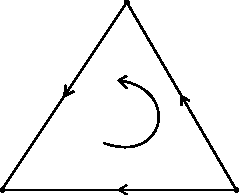
\includegraphics[scale = 0.7]{lectures/0/pictures/pic_1}};
            \node at (0.1, -0.2){\small \( \sigma \)};
            \node at (-0.9, 0){\small \( e_1 \)};
            \node at (1, 0){\small \( e_2 \)};
            \node at (0, -1.3){\small \( e_3 \)};
            \node at (0.2, 1.3){\small \( b \)};
            \node at (-1.4, -1.25){\small \( a \)};
            \node at (1.4, -1.25){\small \( c \)};
            %	\draw[opacity=0.7] \foreach \x in {-4,...,5} {
	   (\x cm, 0.1) -- (\x cm, -0.1) node[below]{\tiny \x}
	   (\x cm - 0.5cm, 0.08) -- (\x cm - 0.5cm, -0.08)
	   \foreach \t in {1,2,3,4,6,7,8,9} {
	      (\x cm - 0.1 * \t cm, 0.055) -- (\x cm - 0.1 * \t cm, -0.055)
	   }
	};
	\draw[opacity=0.7,rotate=90] \foreach \x in {-3,-2,-1,1,2,3,4} {
	   (\x cm, 0.1) -- (\x cm, -0.1) node[right]{\tiny \x}
	   (\x cm - 0.5cm, 0.08) -- (\x cm - 0.5cm, -0.08)
	   \foreach \t in {1,2,3,4,6,7,8,9} {
	      (\x cm - 0.1 * \t cm, 0.055) -- (\x cm - 0.1 * \t cm, -0.055)
	   }
	};

            \end{tikzpicture}
        \end{center}
        Тогда цепной комплекс, построенный по треугольнику будет устроен следующим образом:
        \[ \ldots \to 0 \to \Z \xrightarrow[\sigma \to e_1 + e_2 - e_3]{\partial_{2}} \Z^3 \xrightarrow{\partial_1} \Z^3 \xrightarrow{\varepsilon} \Z \]
        Из ориентации $\sigma$ ясно, что $\partial \sigma = e_1 + e_2 - e_3, \ \partial e_1 = b - c, \ \partial e_2 = a - b, \partial e_3 = a - c$.
        Ясно, что вторые гомологии нулевые:
        \[ H_{2}(X, \Z) = \Ker{\partial_{2}}/0 = 0\]
        Посчитаем теперь первые.
        \begin{multline*} \partial(k_1 e_1 + k_2 e_2 + k_3 e_3) =  k_1(b - c) + k_2(a - b) + k_3(a - c) = a(k_2 + k_3) + b(k_1 - k_2) + c(-k_1 - k_3) \Rightarrow \\ \Rightarrow \Ker\partial_{1} = \langle (k_1, k_2, k_3) \in \Z^3 \ \vert \ k_1 = k_2 = -k_3 \rangle \end{multline*}
        С другой стороны, $\Im{\partial_{2}} = k(e_1 + e_2 - e_3)$. Тем самым, $H_{1}(X, \Z) = 0$. Аналогичным вычислением мы получаем, что $H_{0}(X, \Z) = \Z$.
    \end{example}

    \begin{example}[Спмилициальные гомологии треугольника без внутренности]
        Пусть теперь всё также, как в примере~\ref{ex2}, но у треугольнка нет внутренности.
        Тогда цепной комплекс будет иметь вид
        \[ \ldots \to 0 \to \Z^3 \xrightarrow{} \Z^3 \xrightarrow{} \Z \]
        Из того, как поменялись отображения, ясно, что поменялись только первые гомологии. Теперь $H_{1}(X, \Z) = \Z/\{ 0 \} = \Z$, а
        образующая~--- это цикл $e_1 + e_2 - e_3$. С другой стороны, $\pi_{1}(\Delta) = \Z$.
    \end{example}

    \begin{remark}
       Когда-нибудь позже мы докажем, что для любого симплициального пространства $X$ есть отображение
        \[ \pi_{1}(X) \to H_{1}(X) = \pi_{1}(X)^{ab} = \pi_{1}(X)/[\pi_{1}(X), \pi_{1}(X)].\]
    \end{remark}

    \begin{example}[Симплициальные гомологии тора $\mathbb{T}^2$]
        Рассмотрим двумерный тор $\mathbb{T}^2$, разбитый на симплексы следующим образом:
        \begin{center}
            \begin{tikzpicture}
            \node at (0,0){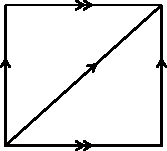
\includegraphics{lectures/0/pictures/pic_2}};
            \node at (-0.5, 0.5){\small \( \sigma_1 \)};
            \node at (0.5, -0.5){\small \( \sigma_2 \)};
            \node at (0.2, -0.2){\small \( e_1 \)};
            \node at (-1.5, 0){\small \( e_2 \)};
            \node at (0, -1.4){\small \( e_3 \)};
            %	\draw[opacity=0.7] \foreach \x in {-4,...,5} {
	   (\x cm, 0.1) -- (\x cm, -0.1) node[below]{\tiny \x}
	   (\x cm - 0.5cm, 0.08) -- (\x cm - 0.5cm, -0.08)
	   \foreach \t in {1,2,3,4,6,7,8,9} {
	      (\x cm - 0.1 * \t cm, 0.055) -- (\x cm - 0.1 * \t cm, -0.055)
	   }
	};
	\draw[opacity=0.7,rotate=90] \foreach \x in {-3,-2,-1,1,2,3,4} {
	   (\x cm, 0.1) -- (\x cm, -0.1) node[right]{\tiny \x}
	   (\x cm - 0.5cm, 0.08) -- (\x cm - 0.5cm, -0.08)
	   \foreach \t in {1,2,3,4,6,7,8,9} {
	      (\x cm - 0.1 * \t cm, 0.055) -- (\x cm - 0.1 * \t cm, -0.055)
	   }
	};

            \end{tikzpicture}
        \end{center}
        Из такой триангуляции ясно, что комплекс будет иметь вид:
        \[ \ldots \to 0 \to \Z^2 \xrightarrow{\partial_{2}} \Z^3 \xrightarrow{\partial_{1}} \Z \xrightarrow{\varepsilon} \Z \]
        Посчитаем дифференциал на двумерных клетках: $\partial{\sigma_1} = e_1 - e_3 - e_2, \ \partial{\sigma_{2}} = e_2 + e_3 - e_1$.
        С другой стороны, ясно, что дифференциал зануляется на любой одномерной клетке, $\partial{e_i} = a - a = 0$.
        \[ H_{2}(\mathbb{T}^2,  \Z) = \Ker{\partial_{2}}/0 = \Z. \]
        так как $\partial{\sigma_{1}} = -\partial{\sigma_{2}} \Rightarrow \Ker{\partial_{2}} = \Z$.

        Также прямыми вычислениями можно убедиться, что $H_{1}(\mathbb{T}^2, \Z) = \Z^2 = \pi_1(\mathbb{T}^2)^{ab}$.
        Образующими первых гомологий будут $e_2$ и $e_3$.

        \noindent\bf{Упражнения.}
        \begin{enumerate}
            \item Посчиать по определению одномерные гомологии связного дерева.
            \item Посчитать по определению все гомологии $n$-мерного симплекса $T^n$
                  \[ T^n \eqdef \left\{ (t_0, \ldots, t_n) \ \vert \ t_i \ge 0, \ \sum_{i = 1}^{n} t_i = 1 \right\}.\]
            \item Покажите, что барицентрическое подразбиение не меняет симплициальных гомологий.
        \end{enumerate}

    \end{example}

    Вообще говоря, далее нужно формально доказывать, что гомологии не зависят от симплициального разбиения пространства (и выяснять, у каких пространств это симплициальное разбиение вообще есть),
    но мы этим всем заниматься не будем, так как в нашем курсе основной будет другая теория.

    \subsection{Сигнулярные гомологии}

    \begin{definition}\label{SingHomology}
        Пусть $X$~--- топологическое пространство.
        \begin{itemize}
            \item \emph{Сингулярным $q$-мерным симплексом} мы будем называть непрерывное отображение $f\colon T^{q} \to X$.
            \item Его граница определяется, как формальная линейная комбинация
                    \[ \partial f \eqdef \sum_{i = 0}^{q} (-1)^i \Gamma_i f,\]
                    где $\Gamma_i f$~--- сужение $f$ на грань $t_i = 0$ (сумма именно такая, так как у $q$-мерного симплекса $q + 1$ грань).
            \item \emph{Сингулярными $q$-мерными цепями} $C_{q}(X, \Z)$ мы будем называть формальные целочисленные линейные комбинации конечного числа $q$-мерных сингулярных симплексов (то есть порожденную ими свободную абелеву группу).
            \item Дифферецниал комплекса\footnote{формально, мы пока еще не знаем, что это комплекс.} $C_{\bullet}$ определяется, как продолжение по линейности оператора взятия границы $q$-мерного сингулярного симплекса.
            \item Комплекс сингулярных цепей может быть снабжен аугументацией $\varepsilon \colon C_{0}\to \Z, \ \sum k_i f_i \to \sum k_i$.
        \end{itemize}
    \end{definition}

    \begin{remark}
       Формально говоря, мы пока не знаем, что комплекс из сингулярных цепей~--- это комплекс. Для этого нам понадобится следующая техническая
    \end{remark}

    \begin{lemma}
        В контексте определения~\ref{SingHomology} $\partial^2 = 0$.
    \end{lemma}
    \begin{proof}
        Посчитаем $\partial \partial f$:
        \[ \partial \partial f = \partial \lr*{\sum_{i} (-1)^i \Gamma_i f} =  \sum_{i, j} (-1)^{i + j} \Gamma_{j}\Gamma_{i}f. \]
        Ясно, что любую грань коразмерности 2 можно получить взятием границы двумя способами.
        Действительно, если $j < i$, то $\Gamma_{i}\Gamma_{j} = \Gamma_{j}\Gamma_{i + 1} $ ($i$-я из оставщихся после выкидывания $j$-й координаты~--- $i+1$-я изначально),
        а в сумме слагаемые $\Gamma_{i}\Gamma_{j}$ и $\Gamma_{j}\Gamma_{i + 1}$ будут с разным знаком, значит $\partial \partial f = 0$.
    \end{proof}

    \begin{definition}
        \emph{Сингулярными гомологиями} топологического пространства $X$ называются гомологии комплекса сингулярных цепей. Мы будем обозначать их, как $H_{k}(X)$ или $H_{\textrm{k}}^{\mathrm{sing}}(X)$.

        В топологическом контексте группу $Z_{q}(X) \eqdef \Ker{\partial_{q}}$ часто называют \emph{$q$-циклами}\footnote{позже мы увидим, какая в этом геометрическая интуиция},
        а группу $B_{q}(X) \eqdef \Im{\partial_{q + 1}}$~--- \emph{q-границами}. В этом смысле $H_{q}(X)$~--- циклы с точностю до границ.
    \end{definition}
    
    \begin{remark}
       Из определения очевидно, что сингулярные гомологии зависят только от класса гомеоморфизма пространства $X$ (их основной плюс и состоит в том, что тут это очевидно). 
    \end{remark}


    

    % Лекция 2 (Сингулярные гомологии точки, категория цепных комплексов и цепные гомотопии, гомотопическая инвариантность гомологий)
        Теперь попробем посчитать по определению сингулярные гомологии для какого-нибудь пространства. 
    Оказывается, что по определению сделать это возможно разве что для точки.

    \begin{theorem}[Сингулярные гомологии точки]
        \[ H_{q}^{\mathrm{sing}}(*, \Z) = 0, \ H_{0}^{\mathrm{sing}}(*, \Z) = \Z, \ \widetilde{H}_{0}^{\mathrm{sing}}(*, \Z) = 0. \]
    \end{theorem}
      Итак, как мы помним, $C_{q}(*)$~--- все линейные комбинации отображений $f\colon T^{q} \to *$.
    Так как отображений из $T^n$ в точку всего одно, $\forall n \ C_{n}(X, \Z)  = \Z$, а значит, наш комплекс
    сингулярных цепей $(C_{\bullet}(*, \Z), \partial)$ будет иметь вид:
    \[ \ldots \Z \xrightarrow{\partial} \Z \xrightarrow{\partial} \ldots \xrightarrow{\partial_2} \Z \xrightarrow{\partial_{1}} \Z \xrightarrow{\varepsilon} \Z. \]
    Теперь посчитаем дифференциалы комплекса.

    Возьмем $f \in C_{1}$, это какая-то формальная линейная комбинация отображений из $[a, b] \to \{ * \}$ Тогда $\partial f$~--- это
    $f\vert_{a} - f\vert_{b} = 0$. Впрочем, и сразу ясно, что в случае любого $n$, так как наше отображение действует в точку (оно постоянно),
    сужения на все грани будут совпадать и результат в сумме будет зависеть лишь от четности $n$, то есть дифференциалы комплекса будут иметь вид:
    \[ \ldots \Z \xrightarrow{\cdot 0} \Z \xrightarrow{\cdot 1} \ldots \xrightarrow{\cdot 1 = \mathrm{id}} \Z \xrightarrow{0} \Z \xrightarrow{\varepsilon} \Z \]
    Иными словами, $\partial_n = 0$, если $n$~--- нечетное и тождественно иначе. Теперь, как нетрудно заметить,
    \[ \forall q > 0 \quad \Ker{\partial_{q}} = \Im{\partial_{q + 1}} \Rightarrow H_{q}^{\mathrm{sing}}(*, \Z) = 0, \ H_{0}^{\mathrm{sing}}(*, \Z) = \Z, \ \widetilde{H}_{0}^{\mathrm{sing}}(*, \Z) = 0. \]


    Трудности, возникшие при подсчетах, намекают на то, что для отрезка, например, это будет сделать еще гораздо труднее.
    С другой стороны, если вдруг окажется, что гомологии гомотопически инвариантны, то мы будем знать, какие гомологии у всех
    стягиваемых пространств (так как для точки мы посчитали).

    В дальнейшем, будем использовать для сингулярных гомологий обозначение $H_{k}$.

    \subsection{Немного гомологической алгеры}

    Рассмотрим категорию цепных комплексов $\fC\fh$ (в нашем случае абелевых групп, но в принципе, всё что тут будет сказано справделиво и в случае $R-\fM\fo\fd$).
    Морфизмом цепных комплексов $(C_{\bullet}, \partial)$ и $(D_{\bullet}, \delta)$ называется набор отображений $f = \{ f_i \}$, где $f_i \in \Hom(C_i, D_i)$ такой, что
    диаграмма
    \begin{center}
        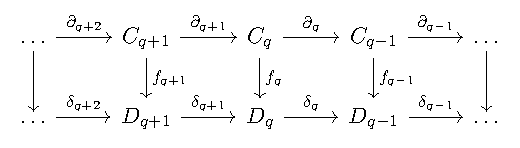
\includegraphics{lectures/0/pictures/cd_1}
    \end{center}
    коммутативна, то есть $\forall i \ f_{i} \circ \partial_{i + 1} = \delta_{i + 1} \circ f_{i + 1}$.

    \begin{lemma}
        Сопоставление цепному комплексу его $k$-й группы гомологий функториально, то есть отображение
        \[ (C_{\bullet}, \partial) \mapsto H_{k}(C_{\bullet}, \delta) \]
        задаёт ковариантный функтор $\fC\fh \to \fA\fb$.
    \end{lemma}
    \begin{proof}
        Всё, кроме того, что композиция переходит в композицию~--- совсем очевидно.
        Нам надо проверить, что отображение $(C_{\bullet}, \partial) \xrightarrow{f} (D_{\bullet}, \delta)$ индуцирует отображение
        $H_{k}(C_{\bullet}) \to H_{k}(D_{\bullet})$, и кроме того,
        \[ (C_{\bullet}, \partial) \xrightarrow{f} (D_{\bullet}, \delta) \xrightarrow{g} (E_{\bullet}, d) \Rightarrow H_{k}(f \circ g) = H_{k}(f) \circ H_{k}(g).\]

        Заметим, что так как $f \in \Hom(C_{\bullet}, D_{\bullet})$, $f_{q}(\Ker{\partial_{q}}) \subset \Ker{\delta_{q}}$.
        Действительно, если $\partial_{q}(x) = 0$, то $0 = f_{q - 1}(\partial_{q}(x)) = \delta_{q}(f_{q}(x)) \Rightarrow f_{q}(x) \in \Ker{\delta_{q}}$.
        Аналогично $f_{q - 1}(\Im{\partial_{q}}) \subset \Im{\delta_{q}}$. Действительно, если $x = \partial_{q}(y)$, то
        \[ f_{q - 1}(x) = f_{q - 1} \circ \delta_{q}(x) = \delta_{q}(f_{q}(y)) \in \Im{\delta_{q}}. \]
        Тогда нужная нам стрелка получается просто из универсального свойства факторгруппы:
        \begin{center}
            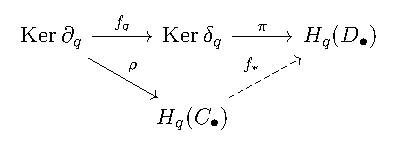
\includegraphics{lectures/0/pictures/cd_2}
        \end{center}
        Действительно, чтоб она существовала, нам нужно, чтоб $\Im{\partial_{q + 1}} \subset \Ker(\pi \circ f_{q})$. Возьмем $x \in \Im{\partial_{q + 1}}$, тогда
        $f_{q}(x) \in \Im_{\delta_{q + 1}} \Rightarrow f_{q}(x) \in \Ker{\pi}$, то есть $x \in \Ker{(\pi \circ f_{q})}$.

        Проверка того, что композиция переходит в композицию тривиальна.
    \end{proof}
    
    \begin{remark}
       Пусть $X, Y \in \fT\fo\fp$, $f\colon X \to Y$~--- непрерывное отображение. Тогда оно индуцирует морфизм
       цепных комплексов $f\colon C_{\bullet}(X) \to C_{\bullet}(Y)$. Действительно, пусть $g \in C_{k}(X)$, тогда $g$~--- это
       непрерывное отображение $T_{k} \to X$ и тогда $f \circ g$~--- непрерывное отображение $T_{k} \to Y$, то есть элемент $C_{k}(Y)$.
       Остается проверить, что полученное отоюражение будет коммутировать с дифференциалом.
       \[ \partial g = \sum_{i = 0}^{k} (-1)^{i} \Gamma_{i}g. \]
       Тогда остается заметить, что взятие грани коммутирует с применением отображения:
       \[ f(\partial{g}) = \sum_{i = 0}^{k} (-1)^{i} \Gamma_{i}f(g) = \partial(f g).   \]

        Значит, если у нас есть непрерывное отображение $f\colon X \to Y$, то есть и индуцированный морфизм гомологий $f_{*}\colon H_{\bullet}(X) \to H_{\bullet}(Y)$.
    \end{remark}   
    
    \begin{statement}
        Если $f\colon X \to Y$~--- гомеоморфизм, то $f_{*}\colon H_{k}(X) \to H_{k}(Y)$~--- изоморфизм (для всех $k$). 
    \end{statement}
    \begin{proof}
        Действительно, если $f$~--- гомеоморфизм, то все индуцированные отображения между цепями~--- изоморфизмы, а значит и все индуцированные отображения в гомологиях
        будут изоморфизмами.
    \end{proof}
    \begin{remark}
       Это утверждение говорит нам о том, что сингулярные гомологии определены для топологических пространств без всякой дополнительной структуры.
    \end{remark}

    \begin{definition}
        Пусть $X$~--- топологическое пространство. Тогда, если группа  $H_{k}(X)$ конечнопорождена, то
        \[ H_{k}(X) \cong \Z^{n} \oplus \mathrm{Tor}(H^{k}(X)). \]
        Тогда число $n$ (то есть, ранг свободной части) называют $k$-м числом Бетти $b_n$. Иными словами, $b_{k}(X) = \rank(H_{k}(X))$.
    \end{definition}

    
    \subsection{Гомотопическая инвариантность гомологий}

    \begin{definition}
        Пусть $(C_{\bullet}, \partial), (D_{\bullet}, \delta) \in \fC\fh$~--- два цепных комплекса. Их морфизмы $f, g \in \Hom_{\fC\fh}((C_{\bullet}, \partial), (D_{\bullet}, \delta))$
        называются \emph{гомотопными} ($f \sim g$), если сущесвует диагональный морфизм $h\colon C_{\bullet} \to D_{\bullet + 1}$ такой, что
        \[ h_{q - 1}\partial_{q} + \delta_{q + 1} h_{q} = f_{q} - g_{q}.  \]
        \begin{center}
            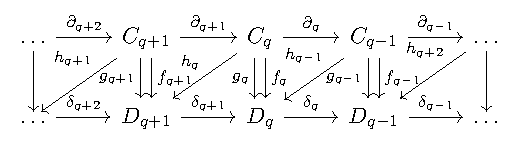
\includegraphics{lectures/0/pictures/cd_3}
        \end{center}
        Кратко это обычно записывают, как $h \partial + \delta h = f - g$.

        Если в категории цепных комплексов $\fC\fh(\fA\fb)$ отождествить гомотопные морфизмы, получится \emph{гомотопическая категория комплексов}, которую обычно обозначают
        $\fK(\fA\fB)$ (или просто $\fK$).
    \end{definition}

    \begin{theorem}\label{HomotopyMorphism}
        Если морфизмы цепных комплексов гомотопны, то есть $f \sim g$, то индуцированные гомоморфизмы когомологий $f_{*} = g_{*}$. Тем самым, функторы гомологий $H_{k}$ пропускаются через гомотопическую категорию.
    \end{theorem}

    \begin{proof}
        Если $x \in \Ker{\partial_{q}}$, то
        \[ f_{q}(x) - g_{q}(x) = \delta_{q + 1} h_{q}(x) + \underbrace{h_{q - 1} \partial_{q}(x)}_{= 0} \in \Im{\delta_{q + 1}},  \]
        а значит в $H_{q}(X)$ эти элементы равны.
    \end{proof}
    \begin{remark}
       Гомотопность морфизмов $f$ и $g$ можно определять, как $\delta h \pm h \partial = f - g$, так как при переходе к гомологиям
       второе слагаемое всё равно обнуляется.
    \end{remark}
    
    \begin{theorem}\label{HomotopyImpliesHomotopy}
        Пусть $f, g\colon X \to Y$, $f \sim g$. Тогда $f_{*} = g_{*}$.
    \end{theorem}
    \begin{proof}
        У нас есть цепные комплексы сингулярных цепей $(C_{\bullet}(X), \partial)$ и $(C_{\bullet}(Y), \partial)$.
        Так как $f \sim g$, существует непрерывное отображение $H\colon X \times I \to Y$, а тогда
        $\forall p\colon T_{q} \to X$ определено непрерывное отобрежение $H(p(\_),\_)\colon T_{q} \times I \to Y$, причем $H(p, 0) = f(p)$
        и $H(p, 1) = g(p)$. Положим
        \[ h(p) = \text{сумма симплексов в разбиении призмы } T_{q} \times I \in C_{q + 1}(Y). \]
        Взглянув на картинку теперь нетрудно заметить, что
        \[ f(p) - h(p) = \text{граница всей призмы} - \text{боковые стенки} = \partial h(p) - h \partial(p) \]
        Таким образом, мы получили, что индуцированные морфизмы цепных комплексов гомотопны, а значит, по теореме~\ref{HomotopyMorphism}, индуцированные
        гомоморфизмы в гомологиях совпадают.
    \end{proof}

    \noindent\bf{Упражнение.}
        Разбить $T_{q} \times I$ на $q + 1$-мерные симплексы формально. А именно, пусть $T_{q} \times \{ 0 \} = a_0 \ldots a_{q}$.
        Пусть вершины $T_{q} \times \{ 1 \}$~--- это $a_0', \ldots, a_q'$. Тогда предлагается брать вершины $a_{0}\ldots a_k a_k' \ldots a_{q}'$.

    \begin{corollary}\label{HomologiesContractible}
        Пусть $X$~--- стягиваемое. Тогда $\widetilde{H}_{\bullet}(X, \Z) = 0$, или, иными словами,
        $\forall k > 0 \ H_{k}(X, \Z) = 0, \ H_{0}(X, \Z) = \Z$.
    \end{corollary}
    
    \noindent\bf{Упражнение.}
        Придумайте пример нестягиваемого $X$ с нулевыми приведёнными гомологиями. 
    
    \begin{lemma}
       Если $X$~--- линейно связно, то $H_{0}(X) = \Z$.
    \end{lemma}
    \begin{proof}
        Выберем в нашем пространстве некоторую фиксированную точку $a$, тогда
        \[ \lr*{\sum k_i f_i} = \lr*{\sum k_i}a \pmod{\Im{\partial_{1}}}, \text{ (то есть, в } H_{0}(X)) \]
        так как все $f_i$ можно соединить путями (а это отображения $T^{1} = [0, 1] \to X$) с $a$ и значит $\Im{\partial_{1}}$ будет содержать
        все разности $f_i - a$. Значит, $H_{0}(X) \cong \Z$.
    \end{proof}

    \begin{corollary}
        Пусть у топологического пространства $X$ $n$ компонент линейной связности. Тогда
        \[ H_{0}(X) \cong \Z^{n}. \]
    \end{corollary}

    \noindent\bf{Упражнение.}
    Дркажите, что непрерывное отображение между линейно связными пространствами индуцирует изоморфизм нулевых гомологий.


    






    

    

    


    % Лекция 3 (Относительные гомологии, гомологически точная последовательность пары)
    \subsection{Относительные гомологии и гомологически точная последовательность пары}

    Пусть $X$~--- топологическое пространство, $A \subset X$, тогда $\forall q \ C_{q}(A) \subset C_{q}(X)$ (вложение индуцирует мономорфизм цепей)
    и мы имеем морфизм цепных комплексов $(C_{\bullet}(X), \partial)$ и $(C_{\bullet}(A), \partial)$, то есть коммутативна следующая диаграмма:
    \begin{center}
        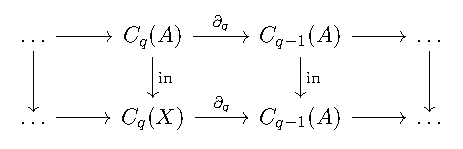
\includegraphics{lectures/0/pictures/cd_4}
    \end{center}
    Это так просто потому, что если у нас был симплекс $f\colon T^{q} \to A$, то его граница тоже целиком лежит в $A$,
    то есть $\partial f\colon T^{q - 1} \to A \in C_{q - 1}(A)$.

    Глядя на это, возникает естественная идея дополнить до короткой точной последовательности
    \[ 0 \to C_{q}(A) \to C_{q}(X) \to C_{q}(X)/C_{q}(A) \to 0 \]
    в каждом столбце.

    \begin{definition}
        Факторгруппу $C_{q}(X, A) \eqdef C_{q}(X)/C_{q}(A)$ называют \emph{относительными цепями}. 
    \end{definition}

    Построим цепной комплекс для относительных цепей, для этого надо определить дифференциалы.
    Это делается стандартно, возьмем $x \in C_{q}(A)$, тогда $\partial_{q}(x) \in C_{q - 1}(A)$, а значит
    композиция дифференциала и проекции пропустится через фактор:

    \begin{center}
        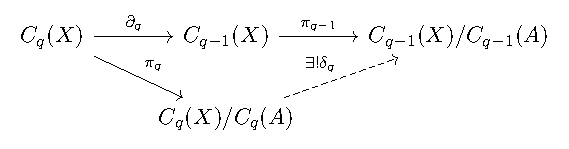
\includegraphics{lectures/0/pictures/cd_5}
    \end{center}

    Проверим теперь, что $\delta^2 = 0$. Действительно, из коммутаивной диаграммы выше мы понимаем, что
    \[ \delta_{q}(\overline{x}) = \delta_{q}(\pi_{q}(x)) = \pi_{q - 1}(\partial_{q}(x)) \Rightarrow \delta_{q - 1}(\delta_{q}(\overline{x})) = \delta_{q - 1}(\pi_{q - 1}(\partial_{q}(x))) = \pi_{q - 2}( \partial_{q - 1}(\partial_{q}(x))) = 0. \]

    Теперь мы построили цепной комплекс и можем определить относительные гомологии.
    \begin{definition}
        Пусть $X \subset A$, тогда относительными гомологиями мы будем называть гомологии комплекса относительных цепей, то есть
        \[ H_{q}(X, A) \eqdef \ker{\delta_{q}}/\Im{\delta_{q + 1}}. \]
    \end{definition}

    Теперь, попробуем получить для гомологий аппарат, идеологически похожий на теорему Зейферта-Ван-Кампена.

    Итак, мы имеем \emph{короткую точную последовательность комплексов}
    \[ 0 \to C_{\bullet}(A) \to C_{\bullet}(X) \to C_{\bullet}(X, A) \to 0\]
    В развёрнутом виде она представляет собой коммутативную диаграмму
    \begin{center}
        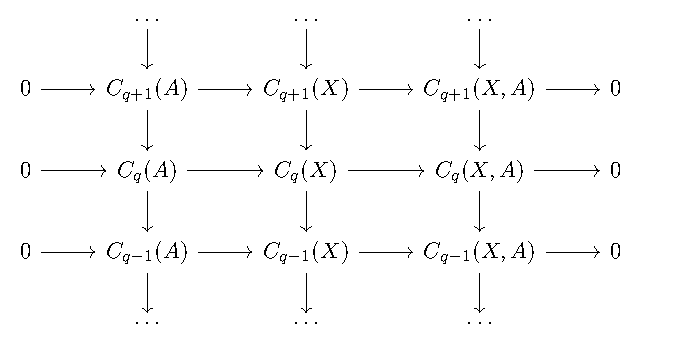
\includegraphics{lectures/0/pictures/cd_6}
    \end{center}
    в которой строки точны, а стлобцы~--- наши комплексы.

    \begin{theorem}[Точная последовательность пары]\label{LongExactSequenceOfPair}
        Существует \emph{связывающий гомоморфизм} $\varphi\colon H_{q}(X, A) \to H_{q - 1}(A)$, и соответственно, имеет место следующая длинная точная последовательность групп гомологий:
        \[ \ldots \to H_{q}(A) \to H_{q}(X) \to H_{q}(X, A) \xrightarrow{\varphi} H_{q - 1}(A) \to H_{q - 1}(X) \to \ldots \]
    \end{theorem}
    \begin{proof}
        На самом деле, это утверждение верно для любой точной последовательности комплексов. А именно, если
        последовательность цепных комплексов
        \[ 0 \to A_{\bullet} \to B_{\bullet} \to C_{\bullet} \to 0\]
        точна, то имеет место следующая длинная точность последовательность гомологий:
        \[ \ldots \to  H_{q}(A) \to H_{q}(B) \to H_{q}(C) \to H_{q - 1}(A) \to H_{q - 1}(B) \to \ldots\]

        Это можно без труда вывести из леммы о змее, проверив точность строк\footnote{\textcolor{magenta}{а так как это делается в абсолютно любом курсе гомологической алгебры, мне лень это сюда писать. }}
    \end{proof}

    \noindent\bf{Упражнение.}
    Докажите, что для $X \supset A \supset B$ имеет место следующая длинная точная последовательность групп гомологий
    \[ \ldots \to H_{q}(A, B) \to H_{q}(X, B) \to H_{q}(X, A) \to H_{q - 1}(A, B) \to \ldots \]

    Посмотрим, что всё это означает геометрически. Относительные циклы~--- это элементы
    \[ \Ker\lr*{C_{q}(X)/X_{q}(A) \to C_{q - 1}(X)/C_{q - 1}(A)}. \]
    Мы взяли представителя в $C_{q}(X)$, взяли границу и после факторизации по $C_{q - 1}(A)$ получили 0,
    а значит граница нашего цикла полностью лежит в $C_{q - 1}(A)$, то есть картинка имеет вид:
    \begin{center}
            \begin{tikzpicture}
            \node at (0,0){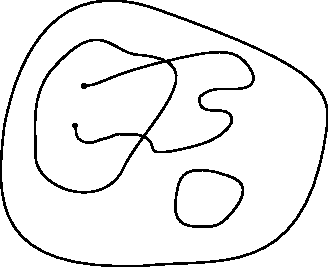
\includegraphics{lectures/0/pictures/pic_3}};
            \node at (-0.5, 0.5){\small \( A \)};
            \node at (3.2, 1.6){\small относительный цикл};
            \node at (-0.5, -1.8){\small абсолютный цикл \( \uparrow \)};
            \node at (1.8, 1.3){\small \( \swarrow \)};
            %	\draw[opacity=0.7] \foreach \x in {-4,...,5} {
	   (\x cm, 0.1) -- (\x cm, -0.1) node[below]{\tiny \x}
	   (\x cm - 0.5cm, 0.08) -- (\x cm - 0.5cm, -0.08)
	   \foreach \t in {1,2,3,4,6,7,8,9} {
	      (\x cm - 0.1 * \t cm, 0.055) -- (\x cm - 0.1 * \t cm, -0.055)
	   }
	};
	\draw[opacity=0.7,rotate=90] \foreach \x in {-3,-2,-1,1,2,3,4} {
	   (\x cm, 0.1) -- (\x cm, -0.1) node[right]{\tiny \x}
	   (\x cm - 0.5cm, 0.08) -- (\x cm - 0.5cm, -0.08)
	   \foreach \t in {1,2,3,4,6,7,8,9} {
	      (\x cm - 0.1 * \t cm, 0.055) -- (\x cm - 0.1 * \t cm, -0.055)
	   }
	};
;
            \end{tikzpicture}
    \end{center}
    С другой стороны, ясно, что $x \in C_{q}(X)/C_{q}(A)$~--- относительная граница, если $x + a = \partial(\ldots)$.

    \begin{remark}
        У связывающего гомоморфизма $H_{q}(X, A) \to H_{q - 1}(A)$ есть очень естественная интерпретация.

    Элементы $H_{q}(X, A)$~--- относительные циклы с точностью до относительных границ. Так как это оносительные $q$-мерные циклы,
    их граница лежит в  $A$, а значит, при взятии границы, мы получим как раз элемент $H_{q - 1}(A)$. То есть, связывающий гомоморфизм
    $H_{q}(X, A) \to H_{q - 1}(A)$~--- взятие границы.
    \end{remark}


    Рассмотрим также еще несколько важных следствий длинной точной последовательности пары. 

    \begin{corollary}\label{ParaCor1}
         Для любого топологического пространства $x$ и любой его точки $x_0 \in X$ мы имеем
        \[ H_{n}(X, x_0) = \widetilde{H}_{n}(X) \ \forall n. \]
    \end{corollary}
    \begin{proof}
        Запишем длинную точную последовательность приведенных гомологий пары $(X, x_0)$
        \[ \ldots \to  \widetilde{H}_{q}(x_0) \to \widetilde{H}_{q}(X) \to \widetilde{H}_{q}(X, x_0) \to \widetilde{H}_{q - 1}(x_0) \to \ldots \]
        Действительно, так как $\widetilde{H}_n(x_0) = 0 \ \forall n$, мы на самом деле имеем
        \[ \ldots \to 0 \to \widetilde{H}_{q}(X) \to \widetilde{H}_{q}(X, x_0) \to 0 \to \ldots, \]
        и из точности следует $\widetilde{H}_{q}(X) \cong \widetilde{H}_{q}(X, x_0) = H_{q}(X, x_0)$.
    \end{proof}

    \begin{corollary}
        Группы $H_{q}(X, A)$ измеряют различие между $H_{q}(X)$ и $H_{q}(A)$, а именно,
        \[ H_{q}(X, A) = 0  \quad \forall{q} \Rightarrow H_{q}(A) = H_{q}(X) \quad \forall q. \]
    \end{corollary}
    \begin{proof}
        Запишем длинную точную последовательность пары $(X, A):$
        \[ \ldots \to  H_{q}(A) \to H_{q}(X) \to H_{q}(X, A) \to H_{q - 1}(A) \to \ldots \]
        В нашем случае она имеет вид:
        \[ \ldots \to  H_{q}(A) \to H_{q}(X) \to H_{q}(X, A) \to H_{q - 1}(A) \to \ldots \]
        и из точности следует, что $H_{q}(A) \cong H_{q}(X)$.
    \end{proof}

    \noindent\bf{Упражнение.} Убедитесь, что верно и обратное утверждение.

    \subsection{Пары Боруска}

    \begin{definition}
        Пусть $X$ -- топологическое пространство, а $A \subset X$ с индуцированной топологией. Тогда говорят, что $(X, A)$ --
        \emph{пара Борсука} (или, \emph{корасслоение})\footnote{Еще говорят <<обладает свойством продолжения гомотопии>>, но это совсем уж длинно.}, если $\forall f \colon X \to Y, \ \forall F \colon A \times I \to Y$ такой, что $F|_{A \times 0} = f|_{A}$
        существует $G\colon X \times I \to Y$, причем такое, что $G|_{X \times 0} = f, \ G|_{A \times I } = F$.
    \end{definition}

    \begin{definition}
        Пара $(X, A)$ называется \emph{клеточной парой}, если $X$~--- клеточное пространство, $A$~--- клеточное подпространство $X$.
    \end{definition}

    \begin{remark}
       Так как очевидно, что $(D^n, \partial D^n)$~--- пара Борсука, клеточная пара является парой Борсука.
    \end{remark}   

    Нам от пар Борсука понадобится несколько базовых утверждений.


    \begin{theorem}[Характеризация пар Борсука]
        Если $(X, A)$~--- пара Борсука, то деформационная ретракция $X \times I$ на $X \cup (A \times I)$.
        Кроме того, если $A$~--- замкнуто, то верно и обратное.
    \end{theorem}
    \begin{proof}
    На картинке это выглядит следующим образом:
        \begin{center}
            \begin{tikzpicture}
            \node at (0,0){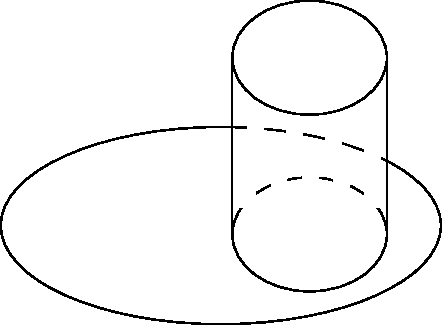
\includegraphics[scale = 0.7]{lectures/0/pictures/pic_4}};
            \node at (2.5, 1){\small \( A \times I \)};
            \node at (-1, -1){\small \( X \)};
            %	\draw[opacity=0.7] \foreach \x in {-4,...,5} {
	   (\x cm, 0.1) -- (\x cm, -0.1) node[below]{\tiny \x}
	   (\x cm - 0.5cm, 0.08) -- (\x cm - 0.5cm, -0.08)
	   \foreach \t in {1,2,3,4,6,7,8,9} {
	      (\x cm - 0.1 * \t cm, 0.055) -- (\x cm - 0.1 * \t cm, -0.055)
	   }
	};
	\draw[opacity=0.7,rotate=90] \foreach \x in {-3,-2,-1,1,2,3,4} {
	   (\x cm, 0.1) -- (\x cm, -0.1) node[right]{\tiny \x}
	   (\x cm - 0.5cm, 0.08) -- (\x cm - 0.5cm, -0.08)
	   \foreach \t in {1,2,3,4,6,7,8,9} {
	      (\x cm - 0.1 * \t cm, 0.055) -- (\x cm - 0.1 * \t cm, -0.055)
	   }
	};

            \end{tikzpicture}
        \end{center}

        Положим $Y = X \cup (A \times I)$, $f\colon X \to Y$~--- вложение. Рассмотрим теперь гомотопию $F_{t}(A) = A \times t$.
        Так как $(X, A)$~--- пара Борсука, существует $G\colon X \times I \to Y\colon G\vert_{A \times I} = F$.

        Докажем теперь в другую сторону:  пусть для $f\colon X \to Y$ есть гомотопия $F_{t}\colon A \to Y$, то
        есть отображение $F\colon X \cup (A \times I) \to Y$. Тогда искомое продолжение гомотопии~---
        композиция $F$ и деформационной ретракции $X \times I \to X \cup (A \times I)$\footnote{вот тут мы пользуемся замкнутостью $A$, так как нам нужно, чтоб покрытие было фундаментальным. }.
    \end{proof}

    \begin{corollary}
        Пара $(D^n, \Int(D^n))$~--- не пара Борсука. 
    \end{corollary}

    Вообще говоря, эта теорема показывает, что было бы хорошо, чтоб  $A$ было замкнутым.

    \begin{remark}
       В нехаусдорфовом случае бывает, что и с незамкнутым $A$ пара $(X, A)$ будет парой Борсука.
    \end{remark}

    \noindent\bf{Упражнение.} Если $(X, A)$~--- пара Борсука и $X$~--- Хаусдорфово, то $A$ замкнуто. 

    \begin{statement}\label{BorsukPairProp}
        Пусть $(X, A)$~--- пара Борсука. Тогда
        \[ X \cup CA \sim (X \cup CA)/CA = X / A.  \]
    \end{statement}
    \begin{proof}
        Рассмотрим вложение $X \to X \cup CA$. Прогомотопируем $A$ в вершину конуса $a$. Так как $(X, A)$~--- пара Борсука,
        эта гомотопия продолжается до гомотопии на $X$. Тогда финальный элемент гомотопии отображает $X \to X \cup CA$ так, что $A \mapsto a$,
        значит, это отображение пропускается через фактор $X/A$. С другой стороны ясно, как устроено обратное отображение $X \cup CA \to X/A$ (стягиваем конус в точку). Нетрудно заметить, что два построенных отображения задают гомотопическую эквивалентность.
    \end{proof}

    \begin{corollary}
         Если $(X, A)$~--- пара Боруска и $A$~--- стягиваемо, то $X \sim X/A$.
    \end{corollary}

    \begin{statement}
        Пара $(CX, X)$~--- всегда пара Борсука.
    \end{statement}

    \subsection{Относительные гомологии как абсолютные (факторизация)}

    Итак, в этом параграфе нас будет интересовать следующее (весьма полезное в вычислениях утверждение):

    \begin{theorem}
        В общем случае отображение $X \to X \cup CA$ индуцирует изоморфизм
        \[ H_{q}(X, A) \to H_{q}(X \cup CA, CA) = H_{q}(X \cup CA, a) = \widetilde{H}_{q}(X \cup CA), \]
        где $a$~--- вершина конуса.

        Если $(X, A)$~--- пара Борсука, то отображение проекции $p\colon X \to X/A, \ A \mapsto a$ индуцирует изоморфизм
        \[ H_{q}(X, A) \xrightarrow{p_{*}} H_{q}(X/A, a) = \widetilde{H}_{q}(X/A). \]
    \end{theorem}

    Вообще говоря, условие на $A$ во второй части теоремы часто опускают и говорят, что это верно для <<хороших пар>>. 
    Мы доказываем для пар Борсука, можно доказывать для случая, когда $A$~--- \emph{окрестностный деформационынй ретракт}.


    Для доказательства этой теоремы нам понадобится несколько важных (в общем контексте) лемм.

    Сначала посмотрим на геометрическую конструкцию \bf{барицентрического подразбиения}, чтоб
    иметь геометрическую интуицию в контексте сингулярных симплексов.

    Рассмотрим симплекс $[v_{0}, \ldots, v_{n}]$. его точки~--- линейные комбинации вида
     \[ \sum_{i = 0}^{n} t_i v_i, \quad \text{где} \sum_{i = 0}^{n} t_i = 1, \ t_i \ge 0. \]
    \begin{definition}
        \emph{Барицентр (центр тяжести)} симплекса~--- это точка $b \in [v_0, \ldots, v_n]$, у которой все барицентрические аоординаты $t_i$ равны, а именно,
        $t_i = \frac{1}{n + 1} \ \forall i$.

        \emph{Барицентрическое подразбиение (подразделение)} симплекса $[v_0, \ldots, v_n]$~--- это разбиение симплекса $[v_0, \ldots, v_n]$ на $n$-мерные симплексы
        $[b, w_0, \ldots, w{n - 1}]$, где по индукции $[w_0, \ldots, w_{n - 1}]$~--- $(n - 1)$-мерный симплекс барицентрического подразбиения грани $[v_0, \ldots, \hat{v}_i, \ldots, v_n]$.
        \begin{itemize}
            \item Индукция начинается с $n = 0$, когда барицентрическое подразбиение точки $[v_0]$ определяется просто, как сама точка $[v_0]$.
            \item В случае $n = 1$
        отрезок $[v_0 v_1]$ бьется на два отрезка $[v_0 b]$, $[b v_1]$, где $b$~--- середина отрезка $[v_0, v_1]$.
            \item В случае $n = 2$ треугольник $[v_0 v_1 v_2]$ бьется на 6 труегольников, образуемых его вершинами и точкой пересечения медиан $b$.
        \end{itemize}

        Из такого индуктивного определения следует, что вершины симплексов в барицентрическом подразбиении симплекса $[v_0 \ldots v_n]$~--- в точности барицентры всех
        $k$-мерных граней $[v_{i_0} \ldots v_{i_k}]$ симплекса $[v_0 \ldots v_n]$ для $0 \le k \le n$.

        При $k = 0$ это даёт нам просто набор вершин $v_i$. Барицентр симплекса $[v_{i_0} \ldots v_{i_k}]$ имеет барицентрические координаты
        $t_i = \frac{1}{k + 1}$ при $i = i_0, \ldots, i_k$ и $t_i = 0$ во всех остальных случаях.

    \end{definition}

    \begin{remark}
       Далее нам это не потребуется, но симплексы барицентрического подразбиения задают на симплексе $T$ структуру симплициального комплекса.
    \end{remark}










    % Лекция 4 (Барицентрическое подразбиение, лемма об измельчении, относительные гомологии, как абсолютные (теорема про H_{q}(X, A) = H_{q}(X/A)))
        \begin{lemma}[О барицентрическом подразбиении]\label{BaricentrLemma}
        Пусть $f\colon T^q \to X$~--- сингулярный симплекс. Тогда его барицентрическое поразбиение~--- это
        \[ \beta\colon C_{q}(X) \to C_{q}(X), \quad  \beta f = \sum_{\tau \in S_{q + 1}}\sign(\tau) f_{\tau}, \]
        где $f_{\tau}$ определяется следующим образом: исходный симплекс $T^{q}$ мы можем барицентрически подразбить на симплексы $T'_{q} = \{ x \ \vert \ x_{\tau(0)} \le x_{\tau(1)} \le \ldots \le x_{\tau(q)}\}$,
        в которых вершины нумеруются согласно размерностям граней. Тогда мы полагаем  $f_{\tau} \eqdef f\vert_{T'_{q}}$.

        Тогда $\partial \beta = \beta \partial$ и  $\beta_{*}([\alpha]) = [\alpha] \ \forall [\alpha] \in H_{q}(X)$. Иными словами,
        барицентрическое подразбиение не влияет на гомологический класс.
    \end{lemma}

    \begin{proof}
        Для первого утверждения достаточно проверить, что в сумме все внутренние грани встречаются с противоположным знаком, это ясно из картинки.
        Первое утверждение даёт нам, что $\beta \in \Hom_{\fC\fh}(C_{\bullet}, C_{\bullet})$.

        Для доказательства второго утверждения мы построим цепную гомотопию $D\colon C_{q}(X) \to C_{q + 1}(X)$ между $\beta$ и постоянным отображением.

        Пусть $f\colon T^{q} \to X$, тогда $D(f)$ определяется следующим образом:
        барицентрически разобьем призму $I \times T^{q}$ на симплексы и рассмотрим проекцию
        \[ p\colon I \times T^q \to T^q. \]
        Тогда $D(f)$~--- это $(q + 1)$-мерный сингулярный симплекс, являющийся суммой композиций $f$ и проекции $p$, суженной на симплексы в разбиении $I \times T^{q}$.
        \begin{center}
            \textcolor{magenta}{можно нарисовать картинку для отрезка, в принципе.}
        \end{center}

        Из того, как устроена нумерация в барицентрическом разбиении призмы, нетрудно видеть, что $D$~--- гомотопия между $\beta$ и $\mathrm{id}$,
        то есть
        \[ f - \beta(f) = D \partial(f) + \partial D(f).  \]
        \textcolor{ForestGreen}{Чтоб понять всё это, надо опять позалипать на эту картиночку с призмой, как в теореме~\ref{HomotopyImpliesHomotopy}.}\footnote{Возможно, всё это место стоит строго формально переписать из Хачтера.}
    \end{proof}

    Следующая лемма говорит нам, что для вычисления сингулярных гомологий достаточно рассматривать лишь \emph{маленькие} сингулярные симплексы.
    В случае симплициальных гомологий это можно было бы формулировать в терминах диаметров, а в случае сингулярных мы будем говорить об этом
    в терминах покрытий.

    \begin{lemma}[Об измельчении]\label{IzmelchLemma}
        Пусть $\cU = \{ U_{\alpha} \}$~--- конечное открытое покрытие $X$.
        Пусть $C_{q}^{\cU}(X)$ порождено сингулярными симплексами $f \in C_{q}(X)$ такими, что $\exists \alpha\colon f(T_{q})  \subset U_{\alpha}$.

        Тогда вложение $i\colon C^{\cU}_{q}(X) \xrightarrow{i} C_{q}(X)$ индуцирует изоморфизм групп гомологий
        $H_{\bullet}(X) \cong H_{\bullet}^{\cU}(X)$.
    \end{lemma}
    \begin{proof}
        Заметим, что для достаточно большого $n$ по лемме Лебега $c \in C_{q}(X) \Rightarrow \beta^n(c) \in C_{q}^{\cU}(X)$.
        Кроме того, по лемме~\ref{BaricentrLemma} $c$ и $\beta^n(c)$ гомологичны (то есть, представляют один м тот же класс гомологий).
        Это даёт нам, что любой гомологический класс мз $H_{q}(C_{\bullet})$ имеет представителя в $C_{q}^{\cU}(X)$, то есть, что
        отображение $H^{\cU}_{q}(X) \to H_{q}(X)$ сюръективно.


        Кроме того, также по лемме~\ref{BaricentrLemma}, если $c$~--- цикл из $C_{q}^{\cU}$, то
        $c - \beta^n(c)$~--- граница цепи из $C_{q + 1}^{U}$, так как
        \[ c - \beta^n(c) =\underbrace{D\partial c}_{ = 0, \text{ так как $c$~--- цикл}} - \partial D c = \partial(-Dc) \in B_{q}\lr*{C_{q}^{\cU}(X)}.\]

        С другой стороны, так как $c$ и $\beta^n(c)$ гомологичны, их разность~--- граница (элемент $B_{q}(C_{q}(X))$).
        Таким образом, если цепь из $C_{q}^{\cU}$ лежит в $B_{q}\lr*{C_{q}(X)}$, то она лежит и в $B_{q}\lr*{C_{q}^{\cU}(X)}$.
        Это даёт нам инъективность отображения $H^{\cU}_{q}(X) \to H_{q}(X)$.
    \end{proof}

    \begin{remark}
       Заметим, что построенные в доказательстве отображения переводят цепи в $A$ в цепи в $A$, а значит, выдерживают факторизацию по $A$.
       Этот факт даёт нам версию леммы об измельчении для относительных гомологий, которым мы и будем пользоваться.
    \end{remark}

    Обзаведемся еще одним полезным фактом:
    Посмотрим на такой факт из гомологической алгебры:

    \begin{lemma}[5-лемма]\label{5-lemma}
        Рассмотрим диаграмму
        \begin{center}
            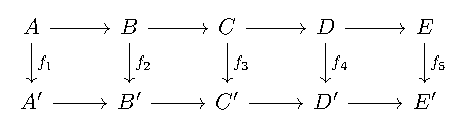
\includegraphics{lectures/0/pictures/cd_7}
        \end{center}
        в которой строки точны, $f_2, f_4$~--- изоморфизмы, $f_1$~--- эпиморфизм, $f_5$~--- мономорфизм.
        Тогда $f_3$~--- изоморфизм.
    \end{lemma}
    \begin{proof}
        Есть в любом курсе гомологической алгебры.
    \end{proof}

    Из неё немедленно следует следующий простой факт:

    \begin{lemma}\label{HomotopyEquivalencePair}
        Если пара $(X, A)$ гомотопически эквивалентна паре $(Y, B)$, то $H_{\bullet}(X, A) = H_{\bullet}(Y, B)$.
    \end{lemma}
    \begin{proof}
        Запишем длинную точную последовательность для обоих пар:
        \begin{center}
            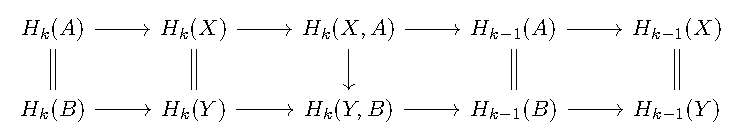
\includegraphics{lectures/0/pictures/cd_8}
        \end{center}
        Тогда всё следует из 5-леммы~\ref{5-lemma}
    \end{proof}

    Наконец, мы можем доказать интересующую нас теорему:

    \begin{theorem}\label{FactorizationTheorem}
        В общем случае отображение $X \to X \cup CA$ индуцирует изоморфизм
        \[ H_{q}(X, A) \to H_{q}(X \cup CA, CA) = H_{q}(X \cup CA, a) = \widetilde{H}_{q}(X \cup CA), \]
        где $a$~--- вершина конуса.

        Если $(X, A)$~--- пара Борсука, то отображение проекции $p\colon X \to X/A, \ A \mapsto a$ индуцирует изоморфизм
        \[ H_{q}(X, A) \xrightarrow{p_{*}} H_{q}(X/A, a) = \widetilde{H}_{q}(X/A). \]
    \end{theorem}

    \begin{proof}
        Рассмотрим открытое покрытие $X \cup CA$ вида:
        \[ X \cup CA \subset ((X \cup CA)\setminus X) \cup (X \cup \overline{C}A), \quad \cU \eqdef \{ (X \cup CA)\setminus X, (X \cup \overline{C}A) \} \]
        где $\overline{C}A$~--- нижняя открытая половина конуса $CA$.

        По лемме~\ref{IzmelchLemma} об измельчении мы вместо $H_{q}(X \cup CA, CA)$ можем рассматривать $H_{q}^{\cU}(X \cup CA, CA)$.

        А теперь, заметим, что по тому, как мы взяли покрытие,
        \[ C_{q}^{\cU}(X \cup CA, CA) = C_{q}^{\cU}(X \cup CA)/C_{q}^{\cU}(CA) = C_{q}\lr*{X \cup \overline{C}A}/C_{q}\lr*{\overline{C}A} = C_{q}\lr*{X \cup \overline{C}A, \overline{C}A}. \]

        А значит, из гомотопической эквивалентности и леммы~\ref{HomotopyEquivalencePair} мы имеем
        \[ H_{q}(X \cup CA, CA) = H_{q}(X \cup \overline{C}A, \overline{C}A) = H_{q}(X, A). \]

        Вторая часть первого равенства из условия теоремы следует из следствия~\ref{ParaCor1}.

        Пусть теперь (X, A)~--- пара Борсука. Тогда по утверждению~\ref{BorsukPairProp} $X \cup CA \sim X/A$, а значит,
        $H_{q}(X, A) \cong \widetilde{H}_{q}(X/A)$.
    \end{proof}

    % Лекция 5 (Вырезание, точная последовательность Майера-Вьеториса, гомологии сфер, гомологии букета и надстройки, гомологии с коэффициентами в абелевой группе)
        \subsection{Вырезание}

    Рассмотрим тройку $B \subset A \subset X$. Тогда вложение индуцирует отображение
    \[ H_{k}(X - B, A - B) \to H_{k}(X, A). \]

    Вообще говоря, вырезание даёт хорошую технику вычисления относительных гомологий:

    \begin{theorem}[О вырезании]\label{CuttingTheorem}
        Пусть даны пространства $Z \subset A \subset X$, причем $\Cl(Z) \subset \Int(A)$. Тогда вложение
        $(X - Z, A - Z) \hookrightarrow (X, A)$ индуцирует изоморфизмы
        \[ H_{n}(X - Z, A - Z) \cong H_{n}(X, A) \]
        для всех $n$. Или, что эквивалентно: для подпространств $A, B \subset X$, внутренности которых покрывают $X$,
        включение $(B, A \cap B) \hookrightarrow (X, A)$  индуцирует изоморфизмы
        \[ H_{n}(B, A \cap B) \cong H_{n}(X, A) \quad \forall n. \]
    \end{theorem}

    \begin{proof}
        Докажем сначала эквивалентность формулировок.  Положим $B = X - Z, \ Z = X - B$.
        Тогда $A \cap B = A - Z$, а условие $\Cl(Z) \subset \Int(A)$ эквивалентно тому, что
        $X = \Int(A) \cup \Int(B)$, так как $X - \Int(B) = \Cl(Z)$. Теперь докажем вторую формулировку.

        Пусть $X = A \cup B$, обозначим соотвествующее покрытие $\cU = \{ A, B \}$. Для краткости будем обозначать группы
        $C^{\cU}_{n}(X)$, как $C_{n}(A + B)$\footnote{что на самом деле логично, так как цепи оттуда состоят из суммы цепей из $A$ и цепей из $B$}.

        Тогда, как мы помним из леммы об измельчении~\ref{IzmelchLemma} включение
        \[ C_{n}(A + B)/C_{n}(A) \hookrightarrow C_{n}(X)/C_{n}(A) \]
        индуцирует изоморфизм групп гомологий $H_{n}(A + B, A) \cong H_{n}(X, A)$.

        Теперь рассмотрим включение
        \[ C_{n}(B)/C_{n}(A \cap B) \hookrightarrow C_{n}(A + B, A). \]
        Оно очевидно индуцирует изоморфизм гомологий, так как обе факторгруппы свободные, а их базис~--- $n$-мерные сингулярные симплексы в $B$, не лежащие в $A$.
        Значит, мы получили требуемый изоморфизм
        \[ H_{n}(B, A \cap B) \cong H_{n}(A + B, A) \cong H_{n}(X, A). \]

    \end{proof}

    \subsection{Точная последовательность Майера-Вьеториса}

    Кроме длинной точной последовательности пары (теорема~\ref{LongExactSequenceOfPair}) для вычисления гомологий пары $(X, A)$
    есть и другая мощная техника для вычисления гомологий пространства $X$, тоже представляющая собой длинную точную последовательность.

    \begin{theorem}[Точная последовательность Майера-Вьеториса, простая версия]\label{Mayer–Vietoris_sequence}
        Пусть $X = A \cup B,$ где $A, B$~--- открытые и $A \cap B  = C \neq \varnothing$.
    Тогда имеет место следующая точная последовательность:
    \[ \ldots  H_{q}(A \cap B) \to H_{q}(A) \oplus H_{q}(B) \to H_{q}(X) \to H_{q - 1}(A \cap B) \to H_{q - 1}(A) \oplus H_{q - 1}(B)  \to \ldots \]
    \end{theorem}
    \begin{proof}
        Рассмотрим короткую точную последовательность  комплексов:
        \[ 0 \to C_{\bullet}(A \cap B) \xrightarrow[\varphi]{c \to (c, -c)} C_{\bullet}(A) \oplus C_{\bullet}(B) \xrightarrow[\psi]{(a, b) \to a + b} C_{\bullet}(A + B) \to 0\]
        Во-первых, заметим, что $\Ker{\varphi} = 0$, так как цепь  в $A \cap B$, которая является нулевой в $A$ (или в $B$) должна быть нулевой цепью.
        Во-вторых, очевидно, что $\psi\varphi = 0 \Rightarrow \Im{\varphi} \subset \Ker{\psi}$. Заметим, что для $(x, y) \in C_{n}(A) \oplus C_{n}(B)$
        имеем $x + y = 0 \Rightarrow y = -x$, а значит $x \in C_{n}(A \cap B)$ и $(x, y) \in \Im{\varphi}$. Это означает, что
        $\Ker{\psi} \subset \Im{\varphi}$. Точность в последнем члене следует просто из определения $C_{n}(A + B)$.

        Тогда эта короткая точная последовательность комплексов даёт нам точную последовательность гомологий. Остается лишь заметить, что
        также, как и в теореме о вырезании, $H_{\bullet}(A + B) = H_{\bullet}(A \cup B)$.
    \end{proof}

    \begin{remark}
       Эта не самая хорошая версия точной последовательности Майера-Вьеториса, так как условие на открытое покрытие серьезно мешает.
    \end{remark}   

    \subsection{Гомологии сфер}

    \begin{theorem}\label{SphereHomology}
        Для $n \neq 0$ гомологии сферы устроены следующим образом:
        \[ H_{i}(S^n) \cong \begin{cases} \Z, \quad i = n  \text{ или } i = n,\\ 0, \quad \text{иначе.}\end{cases} \]
        Или, иными словами,
        \[ \widetilde{H}_{i}(S^n) \cong \begin{cases} \Z, \quad i = n \\ 0, \quad \text{иначе.}\end{cases}\]
    \end{theorem}
    \begin{proof}
        Рассмотрим пару $(X, A) = (D^n, S^{n - 1})$, тогда $X/A \cong S^n$. Запишем для этой пары точную послеоватнльность приведенных гомологий:
        \[ \ldots \to \widetilde{H}_{q}\lr*{D^n} \to \widetilde{H}_{q}\lr*{D^n, S^{n - 1}} \to \widetilde{H}_{q - 1}\lr*{S^{n - 1}} \to \widetilde{H}_{q - 1}\lr*{D^n} \to \ldots \]
        Так как $D^n$ стягиваем, $\widetilde{H}_{q}(D^n) = 0$, а значит, $H_{q}\lr*{D^n, S^{n - 1}} \cong H_{q - 1}(S^n)$. С другой строны, так как $(D^n, \partial D^n) = (D^n, S^{n - 1})$~--- пара Борсука, по теореме о факторизации~\ref{FactorizationTheorem}
        \[ H_{q}\lr*{D^n, S^{n - 1}} \cong \widetilde{H}_{q}\lr*{D^n/S^{n - 1}} \cong \widetilde{H}_{q}\lr*{S^n}. \]

        Остается замеить, что мы знаем, что утверждение верно для $S^0$. Таким образом, мы доказали утверждение по индукции.
    \end{proof}
    
    \begin{corollary}
        Сферы разных размерностей негомеоморфны.
    \end{corollary}

    \subsection{Гомологии букета и надстройки}

    Из стягиваемости конуса сразу следует, что $H_{q}(CX, X) \cong \widetilde{H}_{q}(X)$ (достаточно написать точную последователньность для приведенных гомологий).

    \begin{definition}
        Пусть $X$~--- топологическое пространство. Тогда \emph{надстройкой} над $X$ называется пространство $\Sigma X$,
        определённое, как
        \[ \Sigma X \cong X \times I/\sim, \text{ где } (x, 0) \sim (y, 0) \ \forall x, y \in X \text{ и } (x, 1) \sim (y, 1)  \ \forall x, y \in X. \]
        Иными словами, мы взяли $X \times I$ и стянули $X \times 1$ и $X \times 0$ в точку.
    \end{definition}

    \begin{example}
        Надстройка над окружностью выглядит следующим образом:
        \begin{center}
            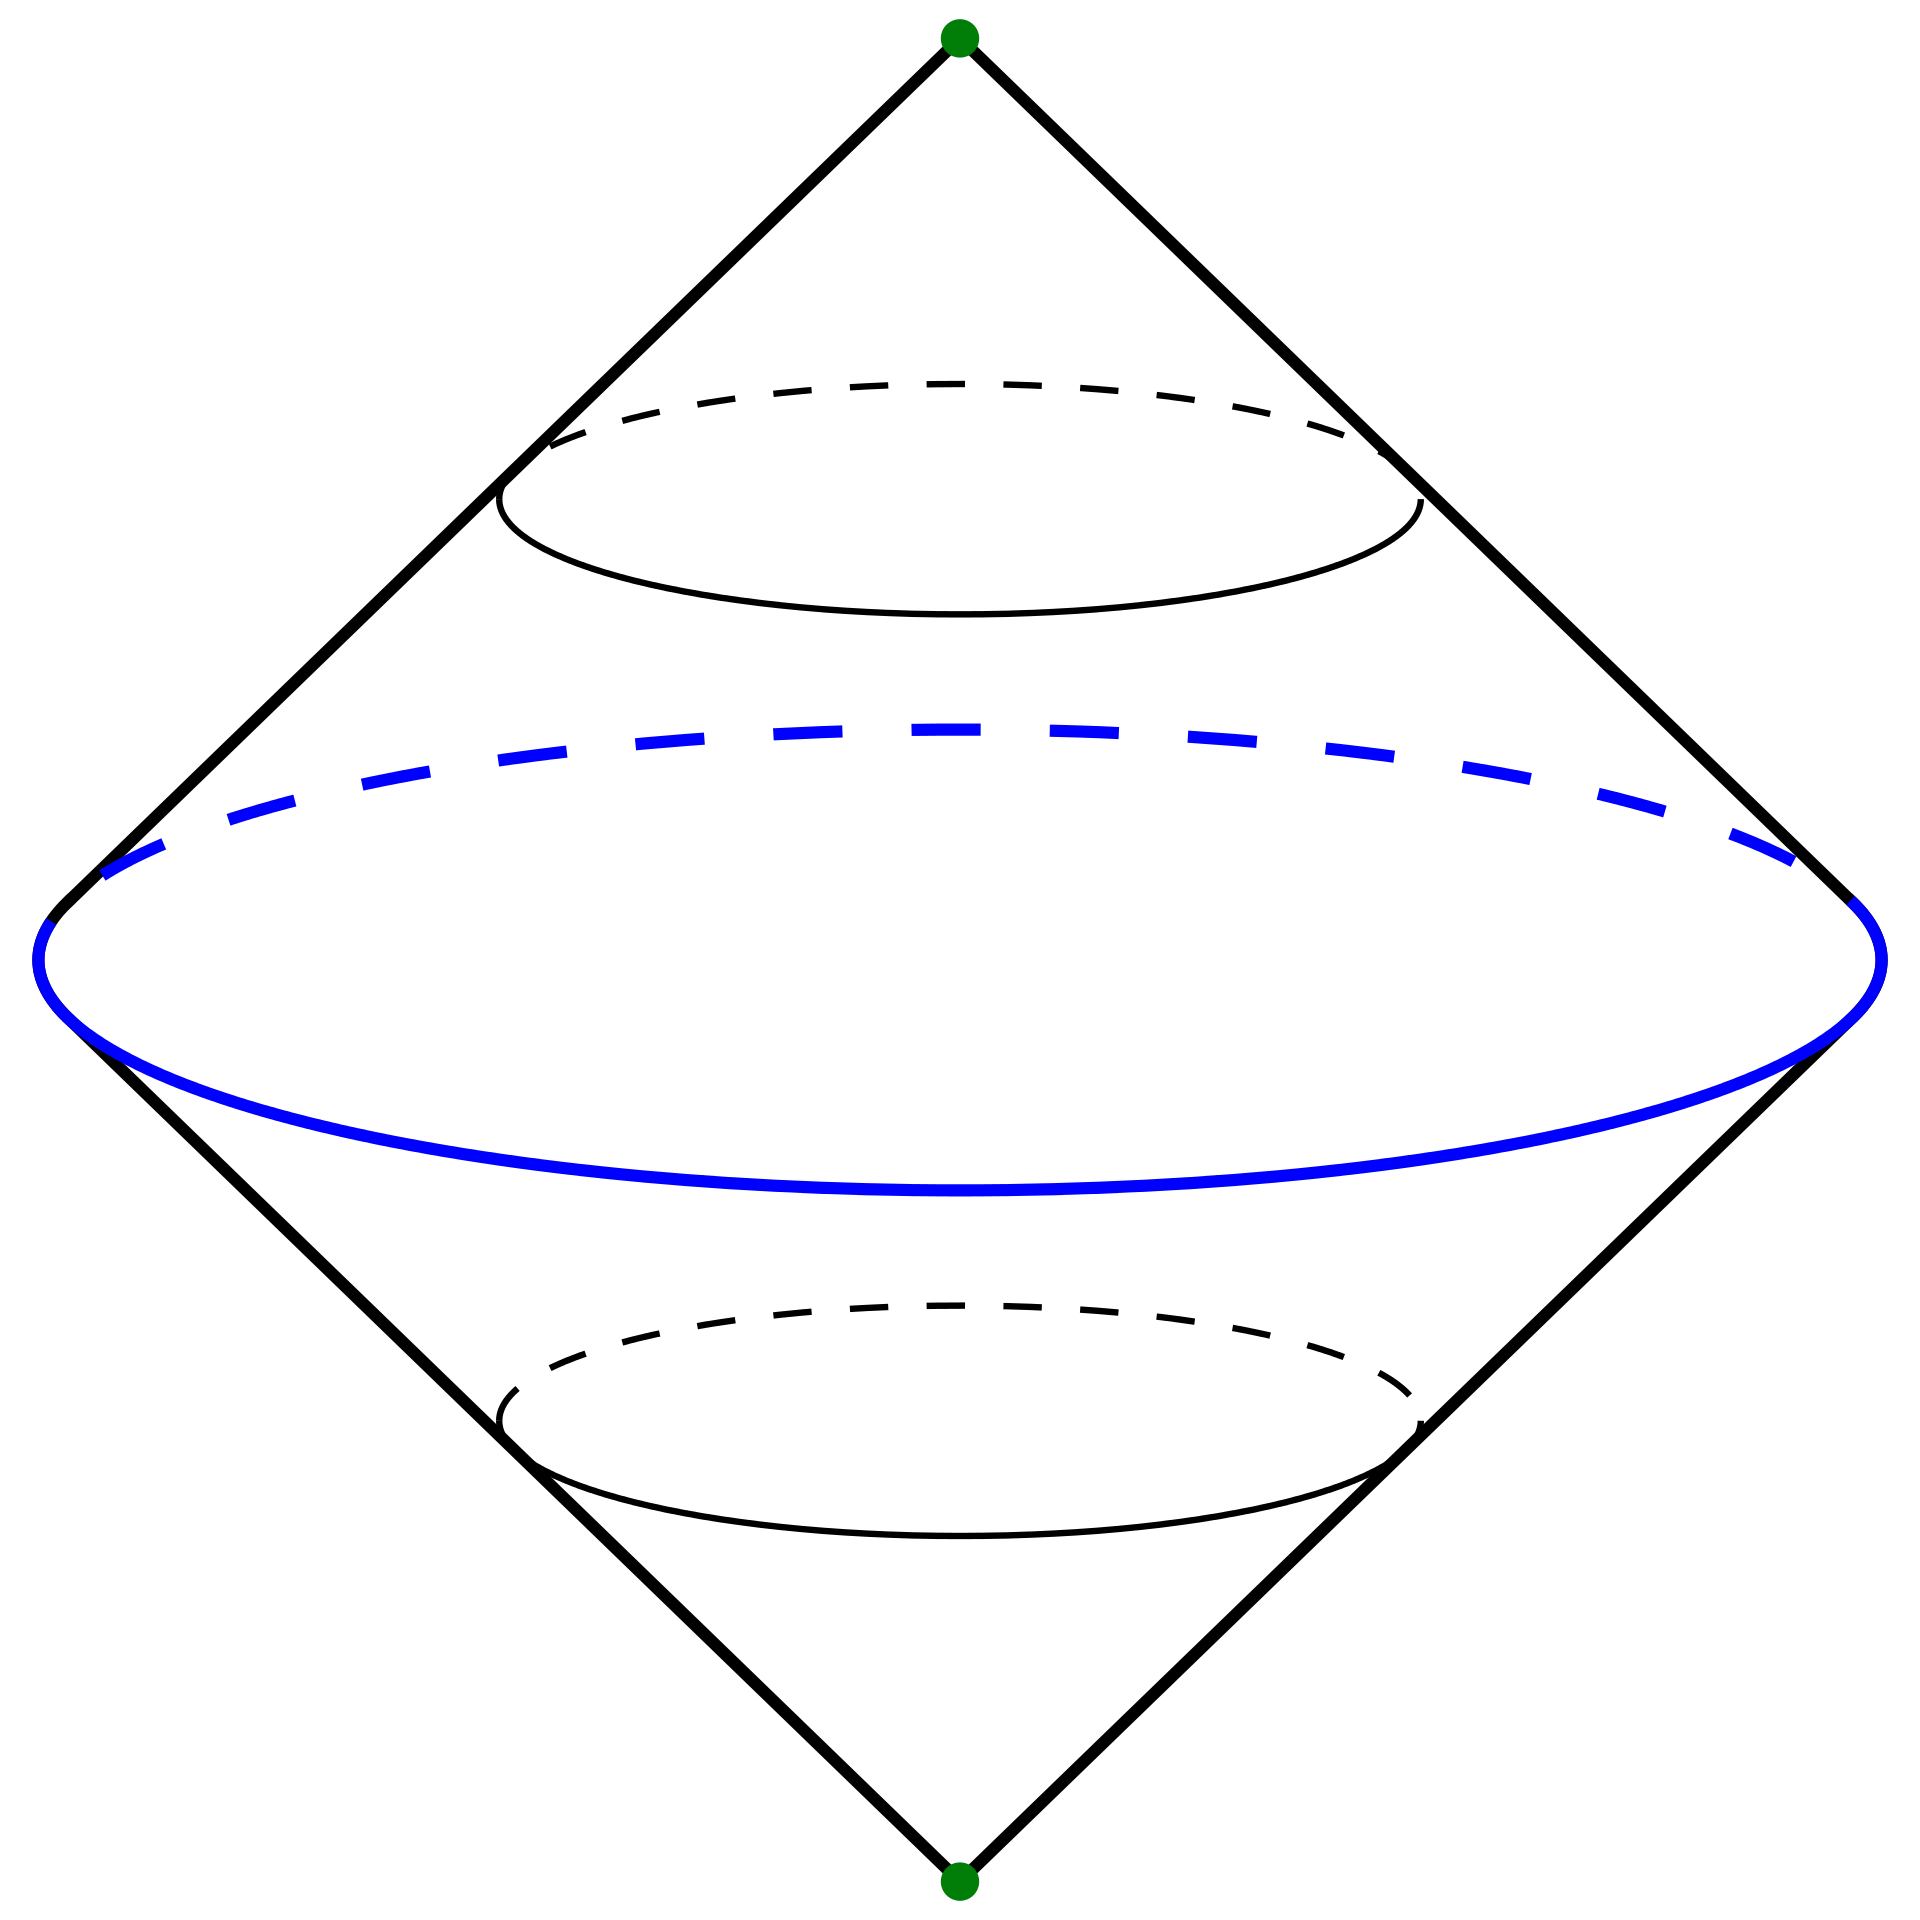
\includegraphics[scale = 0.05]{lectures/0/pictures/pic_5.svg}
        \end{center}
    \end{example}

    Так как надстройка получается факторизацией конуса по нижнему основанию, из теоремы о факторизации~\ref{FactorizationTheorem} следует, что $H_{q + 1}(CX, X) \cong \widetilde{H}_{q + 1}(\Sigma X)$.
    Таким образом, мы получили такое утверждение:
    \begin{theorem}[Гомологии надстройки]
        Справедливо следующее равенство групп гомологий:
        \[ \widetilde{H}_{q}(X) \cong \widetilde{H}_{q + 1}(\Sigma X) \]
    \end{theorem}

    \begin{remark}
       Так как $\Sigma S^n = S^{n + 1}$, мы таким образом получили другое доказательство теоремы~\ref{SphereHomology}.
    \end{remark}

    \begin{theorem}[Гомологии букета]\label{BouqetHomology}
        Для букета пространств $\bigvee_{\alpha} X_{\alpha}$ включения $i_{\alpha}\colon X_{\alpha} \hookrightarrow \bigvee_{\alpha} X_{\alpha}$
        индуцируют изоморфизм гомологий
        \[ \bigoplus_{\alpha} \widetilde{H}_{q} \cong \widetilde{H}_{q}\lr*{\bigvee_{\alpha} X_{\alpha}}. \]
        при условии, что если в букете отождествляются точки $\{ x_{\alpha} \}$, то пары $(X_{\alpha}, x_{\alpha})$~--- пары Борсука.
    \end{theorem}
    \begin{proof}
        Достаточно рассмотреть пару
        \[ (X, A) = \lr*{\bigsqcup_{\alpha} X_{\alpha}, \bigsqcup_{\alpha} x_{\alpha}}, \]
        тогда по тривиальным причинам
        \[ H_{n}(X, A) \cong \bigoplus_{\alpha} \widetilde{H}_{n}(X_{\alpha}) \]
        и по теореме о факторизации
        \[ H_{n}(X, A) \cong \widetilde{H}_{n}\lr*{\bigvee_{\alpha}X_{\alpha}}. \]
    \end{proof}

    \subsection{Гомологии с коэффициентами}

    У рассматриваемой нами до сих пор теории гомологий есть простое обобщение, котрое иногда даёт техническое преимущество.

    Обобщение состоит в рассмотрении цепей $\sum n_i f_i, $ где $f_i$~--- сингулярные симплексы, а коэффициенты $n_i$
    берутся в фиксированной абелевой группе $G$. Такие $n$-мерные цепи образуют абелеву группу $C_{n}(X; G)$ и у неё также есть относительная версия
    $C_{n}(X, A; G) \eqdef C_{n}(X; G)/ C_{n}(A; G)$.

    Дифференциал $\delta$ строится также, как и раньше:
    \[ \partial\lr*{\sum_{i} n_i f_i } = \sum_{i, j} (-1)^j n_i \Gamma_{j}f_i. \]
    Соотвественно, группы $C_{n}(X; G)$ и $C_{n}(X, A; G)$ образуют цепные комплексы и их гомологии обозначают
    $H_{n}(X; G)$ и $H_{n}(X, A; G)$ и называют \emph{гомологиями с коэффициентами в группе $G$}.

    Приведённые группы гомологий $\widetilde{H}(X; G)$ определяются аналогично, аугументация задаётся, как
    \[ \ldots \to C_{0}(X; G) \xrightarrow{\varepsilon} G \to 0, \quad \varepsilon\lr*{\sum_{i} n_i f_i} = \sum_{i} n_i.  \]

    \begin{remark}
       Часто полезно рассматривать гоиологии с коэффициентами в $\Z/2\Z$, так как нужно считать суммы сингулярных симплексов
        с коэффициентами $0$ и $1$, поэтому, отбрасывая члены с коэффициентами $0$, можно представлять себе цепи, как конечные <<объединения>> сингулярных симплексов.

        Кроме того, можно больше не заботиться о знаках в формуле для границы, а так как знаки являются алгебраическим выражением ориентации, мы можем игнорировать и ориентации.
        Это означает, что гомологии с коэффициентами в $\Z/2\Z$~--- наиболее естественный инструмент для вычислений в неориентируемом случае.
    \end{remark}

    Отметим, что вся доказанная выше теория переносится на гомологии с коэффициентами в $G$ без проблем и различия между
    $H_{n}(X; G)$ и $H_{n}(X)$ появляются только, когда начинаются вычисления.

    \begin{example}
        Если $X = *$~--- точка, то нетрудно заметить, что
        \[ H_{n}(*; G) \cong \begin{cases} G, \quad n = 0 \\ 0, \quad \text{иначе} \end{cases}\]

        Аналогично и в случае сфер $S^k$ мы имеем
        \[ \widetilde{H}_{n}(S^k; G) \cong \begin{cases} G, \quad n = k \\ 0, \quad \text{иначе} \end{cases}\]
    \end{example}











    % Лекция 6 (Теорема Брауэра о неподвижной точке, инвариантность размерности, эквивалентность симплициальных и сингулярных гомологий, степень отображения, теорема о Еже, локальность степени)
        \subsection{Приложения теории гомологий}

    \begin{theorem}[Борсук]\label{BorsukTheorem}
        Не существует ретракции диска на граничную сферу.
    \end{theorem}
    \begin{proof}
        Предположим, что ретракция $f\colon D^n \to S^{n - 1}\colon f$~--- непрерывное и $f\vert_{S^{n - 1}} = \mathrm{id}$ существет.
        Рассмотрим отображение $i\colon S^{n - 1} \hookrightarrow D^n$, тогда в гомологиях у нас есть отображение
        \[ H_{n - 1}(S^{n - 1}) \xrightarrow{i_{*}} H_{n - 1}(D^n) \xrightarrow{f_{*}} H_{n - 1}(S^{n - 1}) \]
        или, подставляя известные нам результаты:
        \[ \Z \xrightarrow{i_*} 0 \xrightarrow{f_{*}} \Z. \]
        Так как $f \circ i = \mathrm{id}$, $f_* \circ i_* = \mathrm{id}_* = \mathrm{id}$ и мы приходим к противоречию.
    \end{proof}
    
    \begin{theorem}[Брауэр, о неподвижной точке]
        Пусть $f\colon D^n \to D^n$~--- непрерывное отображение. 
        Тогда у него существует неподвижная точка. 
    \end{theorem}
    \begin{proof}
        Предположим противное, пусть существует непрерывное $f\colon D^n \to D^n$, не имеющее неподвижных точек. Рассмотрим отображение $g$, которое переводит $x \in D^n$
        в точку пересечения $[f(x), x)$ и $\partial D^n$. То есть, $g\colon D^n \to \partial D^n$ и $g\vert_{\partial D^n} = \mathrm{id}$.
        Тогда $g$~--- ретракция $D^n$ на граничную сферу, а этого не бывает по теореме~\ref{BorsukTheorem}.
    \end{proof}
    
    \begin{theorem}[Брауэр, инвариантность размерности]
        Если непустые открытые $U \subset \R^m$, $V \subset \R^n$ открытые и они гомеоморфны, то $m = n$.
    \end{theorem}
    \begin{proof}
        Пусть $h$~--- гомеоморфизм $U \to V$, тогда
        \[ H_{k}(U, U - x) \cong H_{k}(V, V - h(x)). \]
        По теореме о вырезании~\ref{CuttingTheorem} для $(X, A) = (\R^m, \R^m - x)$ и $Z = \R^m - U$:
        \[ H_{k}(\R^m, \R^m - x) \cong H_{k}(U, U - x). \]
        Тогда мы имеем, что
        \[ H_{k}(\R^m, \R^m - x) \cong H_{k}(\R^n, \R^n - h(x)). \]
        Из точной последовательности пары для $(\R^m, \R^m - x)$ мы имеем:
        \[ \ldots \to H_{k}(\R^m) \to H^{k}(\R^m, \R^m - x) \to H_{k - 1}(\R^{m} - x) \to H_{k - 1}(\R^m) \to \ldots \]
        \[ \ldots 0 \to H^{k}(\R^m, \R^m - x) \to H_{k - 1}(\R^{m} - x) \to 0 \to \ldots, \]
        а значит, $H_{k}(\R^m, \R^m - x) \cong H_{k - 1}(\R^m - x) \cong H_{k - 1}(S^{m - 1})$, так как
        $\R^{m} - x$ деформационно ретрагируется на $S^{m - 1}$. Значит, мы получили
        \[ H_{k - 1}(S^{m - 1}) \cong H_{k - 1}(S^{n - 1}), \]
        откуда ясно, что $m = n$.
    \end{proof}

    \subsection{Симплициальные комплексы}

    \textcolor{ForestGreen}{Этот парагарф надо написать из Хатчера}.

    \subsection{Эквивалентность симплициальных и сингулярных гомологий}

    \noindent\bf{Образующая $H_{n}(S^n)$:}

    В этом параграфе будем обозначать $n$-мерный симплекс, как $\Delta^n$. Заметим, что так как $\Delta^n/\partial \Delta^n \cong S^n$, по теореме о факторизации~\ref{FactorizationTheorem}
    мы имеем изоморфизм
    \[ H_{n}\lr*{S^n}\cong H_n\lr*{\Delta^n, \partial \Delta^n}. \]

    Покажем, что образующая $H^{n}(S^n)$~--- это отображение $\Delta^n \xrightarrow{\mathrm{id}} \Delta^n$.
    Нетрудно заметить, что $\Im(\partial f) \subset \partial \Delta^n$, что дает нам, что $\mathrm{id}$ вообще
    представляет какой-то гомологический класс в $H_{n}\lr*{\Delta^n, \partial \Delta^n}$.

    Рассмотрим тройку $\lr*{\Delta^n, \partial \Delta^n, \Lambda}$, где $\Lambda$~--- это
    $\partial \Delta^n$ без одной из граней (например, запоолненный треугольник, граница треугольника и граница треугольника без стороны).
    Напишем точную последовательность тройки:
    \[ \ldots \to H_{n}\lr*{\partial \Delta^n, \Lambda} \to H_{n}\lr*{\Delta^n, \Lambda} \to H_{n}\lr*{\Delta^n, \partial \Delta^n} \to H_{n - 1}\lr*{\partial \Delta^n, \Lambda} \to H_{n - 1}\lr*{\Delta^n, \Lambda} \to \ldots  \]
    Заметим, что так как $\Delta^n$ деформационно ретрагируется на $\Lambda$, $H_{n}\lr*{\Delta^n, \Lambda} \cong H_{n}\lr*{\Lambda, \Lambda} = 0$ и то
    же самое справедливо для $(n - 1)$-х гомологий. То есть, наша последовательность на самом деле имеет вид
    \[ \ldots \to  0 \to H_{n}\lr*{\Delta^n, \partial \Delta^n} \to H_{n - 1}\lr*{\partial \Delta^n, \Lambda} \to 0 \to \ldots  \]
    Теперь заметим, что если грань, которую мы выкинули, мы обозначим за $\Delta'$, то $H_{n - 1}\lr*{\partial \Delta^n, \Lambda} \cong H_{n - 1}\lr*{\Delta', \partial \Delta'}$.

    Это ценно, так как далее мы можем рассуждать по индукции, ведь если образующая $H_{n - 1}\lr*{\Delta', \partial \Delta'}$~--- вложение выкинутой нижней грани $\Delta'$, то
    её прообраз в $H_{n}\lr*{\Delta^n, \partial \Delta^n}$~---- нужное нам тождественное отображение (мы тут пользуемся тем, что
    мы знаем, что связывающий гомоморфизм в длинной точной последовательности пары/тройки~-- это просто взятие границы). А для $S^0$ это утверждение очевидно.

    Обозначим симплиаицльные гомологии пространства $X$ за $H_{k}^{\Delta}(X)$.
    \begin{theorem}
        Пусть $X$~--- конечный симплициальный комплекс. Тогда
        \[ H_{k}^{\mathrm{sing}}(X) \cong H_{k}^{\Delta}(X). \]
    \end{theorem}
    \begin{proof}
        Пусть $X^k$~--- объединение всех симплексов в симплициальном комплексе до размерности $k$ (обозначение аналогично обозначению для $\mathrm{CW}$-комплексов).
        Напишем точную последовательность пары:
        \[ \ldots \to H_{n + 1}^{\Delta}\lr*{X^k, X^{k - 1}} \to H_{n}^{\Delta}\lr*{X^k} \to H_{n}^{\Delta}\lr*{X^k} \to H_{n}^{\Delta}\lr*{X^k, X^{k - 1}} \to \ldots \]
        и заметим, что $H_{n + 1}^{\Delta}\lr*{X^k, X^{k - 1}} \cong H_{n + 1}\lr*{X^k, X^{k - 1}} \cong H_{n + 1}\lr*{\bigvee S^k}$. Действительно, ясно, что
        \[ H_{n + 1}\lr*{X^k, X^{k - 1}} \cong H_{n + 1}\lr*{\bigvee_{\alpha}S^k}, \]
        где $\alpha$ пробегает $k$-мерные симплексы в $X$. Далее,
        \[ H_{n + 1}\lr*{\bigvee_{\alpha}S^k} \cong \begin{cases} 0, \quad \text{ если } n + 1 \neq k \\ \bigoplus_{\alpha} \Z, \quad n + 1 = k \end{cases}\]

        С другой стороны, из определения симплициальных гомологий ясно, что при $n + 1 \neq k$ мы имеем
        $H_{n + 1}^{\Delta}\lr*{X^k, X^{k - 1}} \cong 0$, а при $n + 1 = k$ эта группа~--- свободная абелева группа, порожденная
        всеми $k$-мерными симплексами в $X$, то есть, как и в предыдущем случае
        \[ H_{k}^{\Delta}\lr*{X^k, X^{k - 1}} \cong \bigoplus_{\alpha} \Z. \]
        Остается заметить, что по доказанному в начале параграфа, мы знаем, что у $H_{k}\lr*{\bigvee_{\alpha} S^k}$ такой же набор порождающих.

        Теперь будем вести индукцию по размерности симплициального комплекса. По индукционному предположению мы имеем
        $H_{n}^{\Delta}(X^{k - 1}) \cong H_{n}(X^{k - 1})$ и тогда мы получаем диаграмму из 5-леммы:

        \begin{center}
            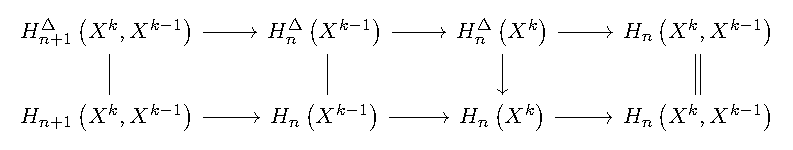
\includegraphics{lectures/0/pictures/cd_9}
        \end{center}
    \end{proof}

    \subsection{Степень отображения}

    \begin{definition}
        Пусть $f\colon S^n \to S^n$~--- непрерывное отображение. Тогда оно индуцирует морфизм в гомологиях:
        \[ f_{*}\colon H_{n}\lr*{S^n} \to H_{n}\lr*{S^n}. \]
        Так как $f_{*}$~--- гомоморфизм бесконечной циклической группы в себя, он должен иметь вид
        \[ f_{*}(\alpha) = d \cdot \alpha \]
        для некоторого фиксированного $d \in \Z$, зависящего только от $f$. Это число называют \emph{степенью отображения $f$}
        и обозначают $\deg{f}$.
    \end{definition}

    \noindent\bf{Базовые свойства степени.}

    \begin{enumerate}
        \item $\deg{\mathrm{id}_{S^n}} = 1$.
        \item Если $f$~--- не сюръекция, то $\deg{f} = 0$, так как мы можем выбрать $x \in S^n\setminus f\lr*{S^n}$  и
        представить $f$ в виде композиции
        \[ S^n \to S^n \setminus \{ x \} \hookrightarrow S^n, \]
        а пространство $S^n \setminus \{ x \}$~--- стягиваемо, значит $H_{n}\lr*{S^n \setminus \{ x \}} = 0$, а значит и $f_{*} = 0$.
        \item Если $f \sim g$, то $\deg{f} = \deg{g}$.
        \item $\deg{f \circ g} = \deg{f} \cdot \deg{g}$.
        \item Если $f$~--- гомотопическая эквивалентность,  то существует $g$ такое, что $f \circ g \sim \mathrm{id} \Rightarrow \deg{f} \deg{g} = 1 \Rightarrow \deg{f} = \pm 1$.
        \item Рассмотрим $f$, которое тождественно действует на первых $n$ координатах и отправляет $x_{n + 1}$ в $-x_{n + 1}$.
        Тогда $\deg{f} = -1$.  Действительно, мы модем реализовать сферу, как склейку двух симплексов $\Delta_{1}^n$ и $\Delta_{2}^n$ по границе.
        Тогда $n$-мерная цепь $\Delta_1^n - \Delta_2^n$ являются образующей $n$-мерных гомологий, а отображение $f$ переставляет местами
        $\Delta_1^n$ и $\Delta_2^n$, то есть действует на образующую умножением на $-1$.
        \item Степень антиподального отображения: $\deg\lr*{x \mapsto -x} = (-1)^{n + 1}$
        \item Если $f \colon S^n \to S^n$ не имеет неподвижных точек, то $f \sim \lr*{x \mapsto -x}$ и соответственно $\deg{f} = (-1)^{n + 1}$.  Действительно, если $f(x) \neq x$, то
        отрезок с концами $f(x)$ и $-x$, который задаётся, как
        \[ t \mapsto (1 - t)f(x) - tx, \ 0 \le t \le 1, \]
        не проходит через начало координат и формула
        \[ H(t, x) = \frac{(1 - t)f(x) - tx}{\| (1 - t)f(x) - tx \|} \]
        определяет гомотопию $f(x)$ в постоянное отображение.
    \end{enumerate}

    \begin{theorem}[О причёсывании ежа]
        $S^n$ допускает непрерывное ненулевое (касательное) векторное поле тогда и только тогда, когда $n$~--- нечетно.
    \end{theorem}
    
    \begin{proof}
        Предположим, что $x \mapsto V(x)$~--- непрерывное поле касательных векторов к сфере. Тогда,
        если рассматривать вектор $V(x)$, как вектор в начале координат, а не в точке касания, то условие касания означает просто, что
        $x \perp V(x)$. Если $V(x) \neq 0$, то мы можем нормализовать веторное поле так, что $\| V(X) \| = 1 \ \forall x$, тогда векторы
        \[ (\cos{t})x  + (\sin{t})V(x) \]
        лежат на единичной окружности в $\Span\lr*{x, V(x)}$.
        Соотвественно, при $t \in [0, \pi]$  мы получаем гомотопию тождественного отображения $\mathrm{id}_{S^n}$ в антиподальное отображение:
        \[ H(t, x) = (\cos{t})x  + (\sin{t})V(x). \]
        Отсюда следует, что $(-1)^{n + 1} = 1$, а значит, $n$ должно быть нечетно. С другой стороны, когда $n = 2k - 1$, мы можем положить
        \[ V(x_1, x_2, \ldots, x_{2k - 1}, 2k) = (-x_2, x_1, \ldots, - x_{2k}, x_{2 k + 1}) \]
        и это даст нам искомое векторное поле.
    \end{proof}

    Опишем теперь метод вычисления, который чаще всего применим на практике.
    Пусть $f\colon S^n \to S^n$ и существует $y \in S^n$ такое, что $f^{-1}(y) = \{ x_1, \ldots, x_k \}$,
    $U_1, \ldots, U_k$~---  непересекающиеся окрестности этих точек, которые $f$ переводит в  окрестность $V$ точки $y$.
    Тогда $f\lr*{U_i \setminus x_i} \subset V \setminus y$ и мы имеем коммутативную диаграмму:
    \begin{center}
        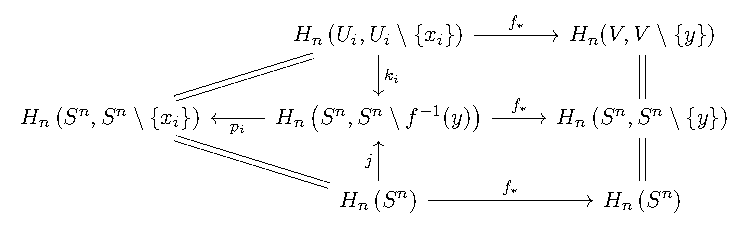
\includegraphics{lectures/0/pictures/cd_10}
    \end{center}

    Все отображения на ней индуцируются включениями. Два ихоморфизма в верхней части диаграммы получаются из теоремы о вырезании~\ref{CuttingTheorem},
    а два в нижней~--- из точной последовательности пары~\ref{LongExactSequenceOfPair}.

    Посредством этих четырех гомоморфизмов две верхние группы можно отождествить с $\Z$, тогда верхний
    гомоморфизм $f_{*}$ становится умножением на число и это число мы будем называть \emph{локальной степенью} отображения $f$
    и обозначать $\deg{f\vert_{x_i}}$.


    \begin{theorem}[Локальность степени]
        Пусть $f\colon S^n \to S^n$ и $y \in S^n$ таково, что $f^{-1}(y) = \{ x_1, \ldots, x_k \}$. Тогда
        \[ \deg{f} = \sum_{i} \deg{f}\vert_{x_i}.\]
    \end{theorem}
    \begin{proof}
        По теореме о выразении~\ref{CuttingTheorem}, группа $H_{n}\lr*{S^n, S^n \setminus f^{-1}(y)}$~--- прямая сумма групп
        $H_{n}\lr*{U_i, U_i \setminus \{ x_i \}}$,  причем $k_i$~--- отображение включения $i$-го слагаемого, а $p_i$~--- проекция на $i$-е слагаемое.
        Из коммутативности нижнего треугольника мы получаем, что
        \[ p_i \circ j (1) = 1, \]
        а значит, $j(1) = (1, \ldots, 1) = \sum_{i} k_i(1)$. Коммутативность верхнего квадрата говорит, что $f_*$ отображает $k_i(1)$ в $\deg{f\vert_{x_i}}$,
        а коммутативность нижнего квадрата уже дает нам формулу
        \[ \deg{f} = \sum_{i} \deg{f\vert_{x_i}}. \]
    \end{proof}
    % Лекция 7 (Клеточные гомологии, теорема сравнения. Приложения клеточных гомологий -- гомологии поверохностей. Пространства Мура (не написал). Теоремы о вложениях дисков и сфер. )
        \subsection{Клеточные гомологии}

    \begin{lemma}
        Пусть $X$~--- конечный $\CW$-комплекс. Тогда:
        \begin{enumerate}
            \item[a)]\label{a} $H_{k}\lr*{X^n, X^{n - 1}} = 0,$ если $k \neq n$ и изоморфно мвободной абелевой группе, если $k = n$.
            Образующие этой группы~--- клетки размерности $n$.
            \item[b)] $H_{k}\lr*{X^n} = 0$, если $k > n$. В частности, если комплекс конечномерен, то $H_{k}(X) = 0 \ \forall k > \dim{X}$.
            \item[c)] Вложение $i\colon X^n \hookrightarrow X$ индуцирует изоморфизм $i_{*}\colon H_{k}(X^n) \to H_{k}(X)$ при $k < n$ и эпиморфизм
            при $k = n$.
        \end{enumerate}
    \end{lemma}
    
    \begin{proof}
        Во-первых, мы знаем, что $\lr*{X^n, X^{n - 1}}$~--- пара Борсука. Кроме того, $X^n/X^{n - 1} \cong \bigvee_{\alpha} S^n$, где $\alpha$ пробегает все $n$-мерные клетки.
        Тогда факт a) следует из теоремы о факторизации~\ref{FactorizationTheorem} и теоремы~\ref{BouqetHomology}.

        Теперь рассмотрим длинную точную последовательность пары
        \[ \ldots \to H_{k + 1}\lr*{X^n, X^{n - 1}} \to H_{k}\lr*{X^{n - 1}} \to H_{k}\lr*{X^n} \to H_{k}\lr*{X^n, X^{n - 1}} \to \ldots. \]
        Если $k \neq n$ или $n - 1$, то обе внешние группы равны нулю, как группы гомологий букета $n$-мерных сфер, поэтому мы получаем изоморфизм
        \[ H_{k}\lr*{X^{n - 1}} \cong H_{k}\lr*{X^n}, \quad k \neq n, n - 1.\]

        Тогда, если $k > n$, то
        \[ H_{k}\lr*{X^n} \cong H_{k}\lr*{X^{n - 1}} \cong \ldots H_{k}\lr*{X^0} = 0, \]
        что доказывает пункт b). Если же $k < m$, то тогда
        \[ H_{k}\lr*{X^n} \cong H_{k}\lr*{X^{n + 1}} \cong \ldots \cong H_{k}\lr*{X^{n + m}} \ \forall m \ge 0,\]
        что доказывает c) в случае конечномерного комплекса. 
    \end{proof}
    
    \begin{remark}
       Утверждение c) верно и для бесконечномерных $\CW$-комплкесов (идея состоит в том, что каждая сингулярная цепь имеет компактный образ, а значит пересекается лишь с конечным числом клеток).
       (Доказательство можно посмотреть в Хатчере).
    \end{remark}

    Теперь мы определим клеточные гомологи~--- более продвинутый способ вычислять гомологии клеточных пространств. Начнем с такой коммутативной диаграммы:

    \begin{center}
        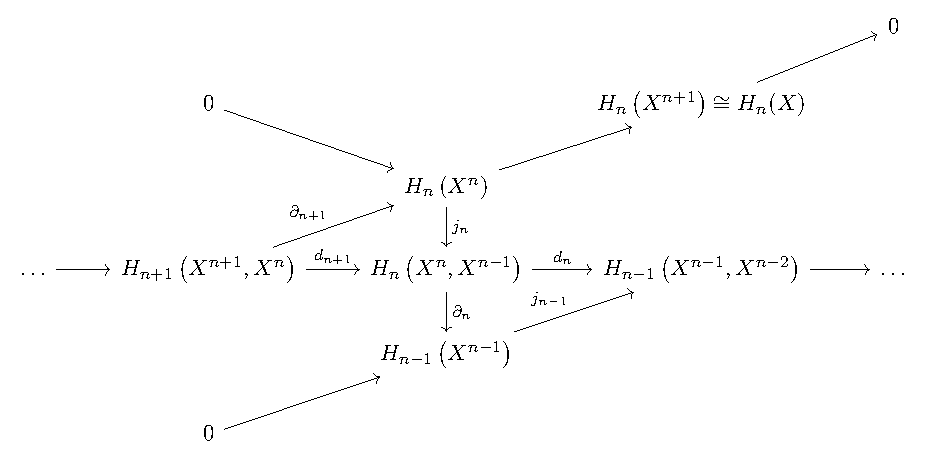
\includegraphics{lectures/0/pictures/cd_11}
    \end{center}

    Её мы получили из точных последовательностей для пар $\lr*{X^{n + 1}, X^{n}}, \lr*{X^n, X^{n - 1}}, \lr*{X^{n - 1}, X^{n - 2}}$.
    Морфизмы в нижней строчке определяются, как $d_{n + 1} \eqdef j_n \circ \partial_{n + 1}$. Нетрудно заметить, что из точности мы получаем $d_n \circ d_{n + 1} = 0$.
    Таким образом, средняя строчка диаграммы является цепным комплексом (его называют \emph{клеточным цепным комплексом для $X$}). Как мы уже замечали в доказательстве леммы выше, группа
    $H_{n}\lr*{X^n, X^{n - 1}}$~--- свободная абелева группа с базисом из $n$-мерных клеток в $X$.

    \begin{definition}
        Рассмотрим построенный выше цепной комлекс с группой $k$-мерных цепей $C_{k}^{\CW}(X) \eqdef H_{k}\lr*{X^k, X^{k - 1}}$. Гомологии этого комплекса называют
        \emph{клеточным гомологиями пространства $X$} и обозначают $H_{n}^{\CW}(X)$.
    \end{definition}

    \begin{remark}
       В самом деле, всё происходящее вполне логично~--- в случае симплициальных гомологий мы рассматриваем свободные абелевы группы, порожденные
        симплексами всех размерностей, а тут~--- клетками всех размерностей. 
    \end{remark}

    \begin{theorem}
        Пусть $X$~--- $\CW$-комплекс. Тогда имеет место изоморфизм $H_{n}^{\CW}(X) \cong H_{n}(X)$.
    \end{theorem}

    \begin{proof}
        Из точности и теоремы о гомоморфимзе мы имеем изоморфизм
        \[ H_{n}(X) \cong H_{n}\lr*{X^n}/\Im{\partial_{n + 1}}.\]
        Так как $j_n$~--- инъекция, $\Im{\partial_{n + 1}} \cong \Im{j_n \circ \partial_{n + 1}} = \Im{d_{n + 1}}$.
        С другой стороны, $\Im{j_n} \cong \Ker{\partial_n}$. Из инъективности $j_{n - 1}$ мы имеем $\Ker{\partial_n} \cong \Ker{d_n}$.
        Значит, $j_n$ индуцирует изоморфизм факторгруппы:
        \[ H_{n}(X) \cong H_{n}\lr*{X^n}/\Im{\partial_{n + 1}} \cong \Ker{d_n}/\Im{d_{n + 1}}. \]
    \end{proof}

    \begin{corollary}\label{CellularHomologyCorollary}
        Пусть $X$~--- $\CW$-комплекс, тогда:
        \begin{enumerate}
            \item $H_{n}\lr*{X} \cong 0$, если в $X$ нет $n$-мерных клеток.
            \item Если $X$~--- $\CW$-комплекс с $k$ клетками размерности $n$, то группа $H_{n}(X)$ порождена не более чем $k$ элементами.
                В самом деле, так как $H_{n}\lr*{X^n, X^{n - 1}}$~--- группа с $k$ образующими, у подгруппы $\Ker{d_n}$ никак не может быть больше образующих, а значит и в факторгруппе
                $\Ker{d_n}/\Im{d_{n + 1}}$ тоже.
            \item Если $X$~--- $\CW$-комплекс, у которого нет пар клеток в соседних размерностях, то $H_{n}(X)$~--- свободная абелева группа с базисом из $n$-мерных клеток.
        \end{enumerate}
    \end{corollary}

    \begin{example}
        Последний пункт следствия~\ref{CellularHomologyCorollary} применим, например, к $\C \mathrm{P}^n$, так как клеточная структура для $\C \mathrm{P}^n$
        имеет по одной клетке каждой четной размерности до $2n$ (действительно, это заметно из того, что $\C \mathrm{P}^n = \C^n \cup \C \mathrm{P}^{n - 1}$). Значит, клеточный цепной комплекс для $\C \mathrm{P}^n$ имеет вид:
        \[ \Z \to 0 \to \Z \to 0 \to \ldots \to 0 \to \Z \to 0 \]
        Также при помощи этого же факта можно посчитать гомологии $S^n \times S^n$.
    \end{example}

    Рассмотрим теперь подробнее клеточный оператор границы $d_n$. При $n = 1$ это легко, так как
    \[ d_1\colon H_{1}\lr*{X^1, X^0} \to H_{0}\lr*{X^0}\]
    и это просто обычное граничное отображение.

    В случае, когда комплекс $X$ связен и имеет лишь одну нульмерную клетку, $d_1 = 0$, так как
    иначе $H_{0}\lr*{X} \neq \Z$. В общем случае формула для клеточного оператора границы имеет следующий вид:

    \begin{statement}
        Имеет место равенство:
        \[ d_n\lr*{e_{\alpha}^n} = \sum_{\beta} d_{\alpha \beta} e_{\beta}^{n - 1}, \]
        где $d_{\alpha \beta}$~--- степень отображения $S^{n - 1}_{\alpha} \to X^{n - 1} \to S_{\beta}^{n - 1}$, которое является композицией
        отображения приклеивания клетки $e_{\alpha}^n$ по границе и отображения фаткоризации, стягивающего $X^{n - 1}\setminus e_{\beta}^{n - 1}$ в точку.
    \end{statement}

    \begin{proof}
        Для получения этой формулы рассмотрим такую коммутативную диаграмму:
        \begin{center}
            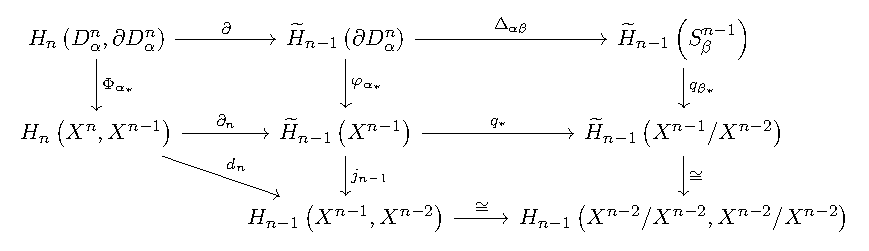
\includegraphics{lectures/0/pictures/cd_12}
        \end{center}
        Проясним, что за стрелки на ней:
        \begin{itemize}
            \item $\Phi_{\alpha}$~--- характеристическое отображение клетки $e_{\alpha}^n$, $\varphi_{\alpha}$~--- её отображение приклеивания.
            \item $q\colon X^{n - 1} \to X^{n - 1}/X^{n - 2}$~--- отображение факторизации.
            \item $q_{\beta}\colon X^{n - 1}/X^{n - 2} \to S_{\beta}^{n - 2}$~--- стягивание дополнения клетки $e_{\beta}^{n - 1}$ в точку и отождествление
            получишейся сферы с $S_{\beta}^{n - 1} = D_{\beta}^{n - 1}/\partial D_{\beta}^{n - 1}$.
            \item $\Delta_{\alpha \beta} = q_{\beta} q \varphi_{\alpha}$.
        \end{itemize}

        Отображение $\Phi_{\alpha_{*}}$ переводит образующую $[D_{\alpha}^n] \in H_{n}\lr*{D_{\alpha}^n, \partial D_{\alpha}^n}$ в образующую слагаемого
        $\Z$ группы $H_{n}\lr*{X^n, X^{n - 1}}$, соответствующего клетке $e_{\alpha}^n$ (действительно, такие клетки образуют базис $H_{n}\lr*{X^n, X^{n - 1}}$).
        Коммутативность левой половины диаграммы даёт нам, что
        \[ d_{n}\lr*{e_{\alpha}^n} = j_{n - 1}\varphi_{\alpha_{*}}\partial [D_{\alpha}^n]. \]

        Базис группы $H_{n - 1}\lr*{X^{n - 1}, X^{n - 2}}$ состоит из $(n - 1)$-мерных клеток, а отображение $q_{\beta_{*}}$~--- это проекция группы
        $\widetilde{H}_{n - 1}\lr*{X^{n - 1}/X^{n - 2}}$ (которая, как группа гомологий букета окружностей суть прямая сумма $\Z$, где каждое слагаемое соотвествует $(n - 1)$-мерной клетке)
        на её слагаемое $\Z$, соответсвующее $e_{\beta}^{n - 1}$.

        Теперь формула следует непосредственно из коммутативности правой верхней части диаграммы7
    \end{proof}


    \subsection{Гомологии поверхностей}

    В данном параграфе, пользуясь клеточными гомологиями, мы вычислим гомологии поверхностей.

    Пусть $M_{g}$~--- компактная ориентируемая поверхность с $g$ ручками. Реализуем её, как склейку $4g$-угольника:
    \begin{center}
            \begin{tikzpicture}
            \node at (0,0){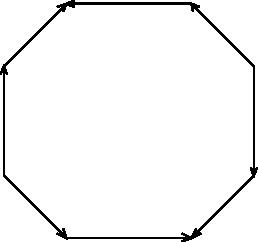
\includegraphics{lectures/0/pictures/pic_5}};
            \node at (-2.3, 0){\small \( a \)};
            \node at (2.3, 0){\small \( c \)};
            \node at (-1.75, 1.6){\small \( b \)};
            \node at (0, 2.2){\small \( a \)};
            \node at (0, -2.2){\small \( c \)};
            \node at (1.75, 1.6){\small \( b \)};
            \node at (1.75, -1.6){\small \( d \)};
            \node at (-1.75, -1.6){\small \( d \)};
            %	\draw[opacity=0.7] \foreach \x in {-4,...,5} {
	   (\x cm, 0.1) -- (\x cm, -0.1) node[below]{\tiny \x}
	   (\x cm - 0.5cm, 0.08) -- (\x cm - 0.5cm, -0.08)
	   \foreach \t in {1,2,3,4,6,7,8,9} {
	      (\x cm - 0.1 * \t cm, 0.055) -- (\x cm - 0.1 * \t cm, -0.055)
	   }
	};
	\draw[opacity=0.7,rotate=90] \foreach \x in {-3,-2,-1,1,2,3,4} {
	   (\x cm, 0.1) -- (\x cm, -0.1) node[right]{\tiny \x}
	   (\x cm - 0.5cm, 0.08) -- (\x cm - 0.5cm, -0.08)
	   \foreach \t in {1,2,3,4,6,7,8,9} {
	      (\x cm - 0.1 * \t cm, 0.055) -- (\x cm - 0.1 * \t cm, -0.055)
	   }
	};
;
            \end{tikzpicture}
    \end{center}

    Тогда в её клеточном разбиении:
    \begin{itemize}
        \item 1 двумерная клетка, приклеенная по произведению коммутаторов $[a_1, b_1] \ldots [a_{g}, b_{g}]$.
        \item $2g$ одномерных клеток.
        \item 1 нульмерная клетка.
    \end{itemize}

    Значит, цепной клеточный комплекс для $M_g$ будет иметь вид:
    \[ 0 \to \Z \xrightarrow{d_2} \Z^{2g} \xrightarrow{d_1} \Z \to 0 \]

    Так как комплекс связен и имеет лишь одну нульмерную клетку, $d_1 = 0$. Кроме того, каждое ребро $[a_1, a_2], \ [a_{g}, b_{g}]$
    появляется в произведении коммутаторов вместе со своим обратным, а значит, $\Delta_{\alpha \beta}$ гомотопны постоянным отображениям, из чего следует, что $d_{2} = 0$.

    Таким образом, мы имеем
    \[ H_{k}\lr*{M_{g}} = \begin{cases} \Z, \quad k = 0 \text{ или } k = 2, \\ \Z^{2g}, \quad k = 1 \\ 0, \quad \text{иначе}\end{cases}\]

    Теперь вычислим гомологии неориентируемой замкнутой поверхности рода $g$. Она имеет такую клеточную структуру:
    \begin{itemize}
        \item Одна нульмерная клетка.
        \item $g$ одномерных клеток.
        \item Одна двумерная клетка, приклеенная по слову $a_{1}^{2}\ldots a_{g}^{2}$.
    \end{itemize}
    Тогда клеточный цепной комплекс имеет вид:
    \[ 0 \to \Z \xrightarrow{d_2} \Z^{g} \xrightarrow{d_1} \Z \to 0 \]
    Аналогично предыдущему разу, $d_{1} = 0$, а вот $d_{2}$ задаётся уравнением
    \[ d_{2}(1) = (2, \ldots, 2), \]
    так как  каждое ребро $a_i$ появляется в слове приклеивания двумерной клетки со степенью 2, а это значит, что каждое отображение
    $\Delta_{\alpha \beta}$ гомотопно отображению степени 2. Значит, $d_{2}$ инъективно и
    \[ H_{2}(N_{g}) = 0. \]

    Выберем в $\Z^{g}$ такой базис: $(1, 0, \ldots, 0), (0, 1, 0, \ldots, 0), \ldots, (0, \ldots, 1, 0), (1, 1, \ldots 1)$. Тогда нетрудно заметить, что
    \[ H_{1}\lr*{N_{g}} \cong \Z^{g - 1} \oplus \Z/2\Z. \]

    \subsection{Пространства Мура}

    Допишу позже вместе с пространствами Эйленберга-Маклейна.

    \subsection{Теорема о вложении дисков и сфер}

    Напомним, что топологическое вложение~--- гомеоморфизм на образ.

    \begin{theorem}
        Пусть $h\colon D^k \to S^n$~--- вложение. Тогда
        \[ \widetilde{H}_{i}\lr*{S^n \setminus h\lr*{D^k}} = 0 \ \forall i. \]
        Кроме того, если $h\colon S^k \to S^n$~--- вложение (и $k < n$), то
        \[ \widetilde{H}_{i}\lr*{S^n \setminus h\lr*{S^k}} = \Z, \ i = n - k - 1 \text{ и } 0 \text{ иначе. }\]
    \end{theorem}
    \begin{proof}
        Проведём индукцию по $k$. Случай $k = 0$ тривиален:
        \[ S^n \setminus h\lr*{D^0} = \R^n. \]
        Теперь докажем индукционный переход от противного. Рассмотрим покрытие нашего пространства двумя множествами:
        \[ A = S^n \setminus h\lr*{I^k \times \left[0, \frac{1}{2}\right]}, \quad B = S^n \setminus h\lr*{I^k \times \left[\frac{1}{2}, 1\right]}. \]
        Заметим, что $A \cup B = S^n \setminus \lr*{h\lr*{I^k \times \left[0, \frac{1}{2}\right]} \cap h\lr*{I^k \times \left[\frac{1}{2}, 1\right]}} = S^n \setminus h\lr*{I^k \times \frac{1}{2}}$ и
        \[ \widetilde{H}_{i}(A \cup B) \cong \widetilde{H}_{i}\lr*{S^n \setminus h\lr*{I^k \times \frac{1}{2}}} = 0,\]
        по индукционному предположению.
        Напишем теперь точную последовательность Майера-Вьеториса (\ref{Mayer–Vietoris_sequence}):
        \[ \ldots \to H_{n}(A \cap B) \to H_{n}(A) \oplus H_{n}(B) \to H_{n}(X) \to H_{n - 1}(A \cap B) \to \ldots \]
        \[\ldots \to  H_{n}\lr*{S^n \setminus h\lr*{I^{k + 1}}} \to H_{n}(A) \oplus H_{n}(B) \to \underbrace{H_{n}\lr*{S^n \setminus h\lr*{I^k \times \frac{1}{2}}}}_{\cong 0} \to H_{n - 1}\lr*{S^n \setminus h\lr*{I^{k + 1}}} \to \ldots \]
        \[ \]
        значит если в $\widetilde{H}_{i}\lr*{A \cap B} = \widetilde{H}_{i}\lr*{S^n \setminus \lr*{I^{k} \times I}}$ есть ненулевой класс $a$, его образ $(a, -a)$ в  $\widetilde{H}_n(A) \oplus \widetilde{H}_n(B)$ будет ненулевым, а значит, в  $\widetilde{H}_{i}(A)$ или $\widetilde{H}_{i}(B)$  тоже будет ненулевым.
        Далее мы можем также разбить на две части интервал в $A$ или в $B$ (в зависимости от того, где не ноль) и проделать всё полностью аналогично.
        Таким образом мы получим последовательность вложенных интервалов $I_n$ таких, что
        \[ \widetilde{H}_{i}\lr*{S^n \setminus h\lr*{I^{k} \times I_n}} \neq 0, \ a \in \widetilde{H}_{i}\lr*{S^n \setminus h\lr*{I^{k} \times I_n}}. \]
        Тогда, если $p = \bigcap I_n$, то по индукционному предположению
        \[ \widetilde{H}_{i}\lr*{S^n \setminus h\lr*{I^k \times p}},  \]
        то есть $a$ представляет ноль в этих гомологиях. Но это означает, что он является чьей-то границей, но тогда он является границей и в допредельном случае, что даёт нам противоречие.

        Докажем теперь второй пункт. Представим сферу ввиде объединения двух дисков (полусфер):
        \[ S^k = D^k_{+} \cup D^k_{-}, \quad D_{-}^{k} \cap D_{+}^{k} = S^{k - 1}. \]
        тогда $S^n \setminus h\lr*{S^k} = S^n \setminus h\lr*{D^{k}_{+} \cup D^{k}_{-}} = S^n \setminus h\lr*{D_{-}^k} \cap S^n \setminus h\lr*{D_{+}^k}$.
        Запишем опять точную последовательность Майера-Вьеториса~\ref{Mayer–Vietoris_sequence}, полагая
        \[ A = S^n \setminus h\lr*{D_{+}^k}, \quad B = S^n \setminus h\lr*{D_{+}^k}. \]:
        \[ \ldots \to H_{i}\lr*{S^n \setminus h\lr*{S^{k}}} \to \underbrace{H_{i}\lr*{S^n \setminus h\lr*{D^k_{-}}}}_{= 0} \oplus \underbrace{H_{i}\lr*{S^n \setminus h\lr*{D^k_{+}}}}_{= 0} \to H_{i}\lr*{S^n \setminus h\lr*{S^{k - 1}}} \to \ldots  \]
        Нулевые элементы в точной последовательности у нас их первого утверждения теоремы. Теперь видно, что мы можем вести индукцию по $k$.
    \end{proof}


    % Лекция 8 -- закрытие дыр за прошлые лекции. 
    % Лекция 9 (Определение когомологий, умножение в когомологиях)
        \subsection{Когомологии}

    Итак, рассмотрим цепной комплекс абелевых групп $(C_{\bullet}, \partial)$
    \[ \ldots \to C_{k} \to C_{k - 1} \to C_{k - 2} \to \ldots \]
    Тогда мы можем рассмотреть группы $C^{k} \eqdef \Hom\lr*{C_{k}, G}$, где $G$~--- фиксированная абелева группа.\footnote{В нашем, топологическом контексте, это группа коэффициентов.}
    Тогда мы получаем цепной комплекс
    \[ \ldots \leftarrow C^{k + 1} \xleftarrow{\delta} C^{k} \xleftarrow{\delta} C^{k - 1} \xleftarrow{\delta} \ldots \]
    Естественно, стрелки развернулись, так как мы подействовали на комплекс контравариантным функтором $\Hom(\_, G)$.
    Действие оператора $\delta$ определяется естественным образом:
    \[ \varphi \in C^{k}, \ \delta\varphi\colon C_{k + 1} \xrightarrow{\partial} C_{k} \xrightarrow{\varphi} G, \ \delta\varphi = \varphi \circ \partial. \]
    \begin{remark}
       Сразу же нетрудно заметить, что $\delta^2 = 0$, то есть построенный комплекс действительно будет комплексом. Действительно,
        \[ \delta_{k} \circ \delta_{k - 1}(\varphi(c)) = \delta_k(\varphi(\partial_{k - 1}c)) = \varphi(\partial_{k}\partial_{k - 1}c) = 0. \]
    \end{remark}

    \begin{definition}
        Группы гомологий коцепного комплекса $(C^{\bullet}, \delta) = (\Hom(C_{\bullet}), G), \delta)$ называют \emph{группами когомологий} комплекса $(C_{\bullet}, \partial)$ с коэффициентами в группе $G$ и обозначаются
    $H^{k}(C_{\bullet}; G)$. Как и в случае с гомологиями, $\Im{\delta_k}$ называют $k$-мерными кограницами, $\Ker{\delta_{k}}$~--- $k$-мерными коциклами, а  $C^k$~--- $k$-мерными коцепями.
    \end{definition}

    Таким образом, мы определили и \emph{сингулярные когомологии} пространства  $X$ (так как они строятся по сингулярным гомологиям).
    Заметим, что так как функтор $\Hom$ контравариантен, логично ожидать, что и когомологии будут контраваринатным функтором. Действительно,
    если $f\colon X \to Y$~--- непрерывное отображение, то у нас есть индуцированный морфизм
    \[ f_{*} \colon C_{k}(X) \to C_{k}(Y) \]
    и действием функтора $\Hom$ мы получаем индуцированный морфизм $f^{*}\colon C^{k}(Y) \to C^{k}(X)$:
    \[  \varphi \in C^{k}(Y), \ \varphi \colon C^{k}(Y) \to G, \ f^{*}(\varphi) \eqdef \varphi \circ f \colon C^{k}(X) \to G, \ f^{*}(\varphi) \in C^{k}(X). \]
    Покажем теперь, что у нас будет и индуцированный морфизм в когомологиях:
    \[ f^{*}\colon H^{k}(Y) \to H^{k}(X) \]
    Для этого надо проверить, что  отображение уважает добавление кограницы, то есть, если мы выберем
    другого представителя того же когомологического класса, мы полужем тот же образ, что и до этого. Действительно,
    \[ f^{*}(c_k + \delta c_{k - 1}) = f^{*}(c_k) + \delta f^{*}(c_{k - 1}) \]

    \begin{remark}
       Формально, как и в гомологиях, нам надо проверить, что $f^{*}\delta = \delta f^{*}$. Действительно, пусть $\varphi \in C^{k}(X)$, тогда
        \[ f^{*}(\delta \varphi) = f^{*}(\varphi  \partial)  = \varphi \partial f = \varphi f \partial = \delta f^{*}(\varphi). \]
        В третьем равенстве мы пользуемся тем, что в начале курса мы уже проверяли, что граничный оператор коммутирует с непрерывными отображениями.
    \end{remark}

    \subsection{Формула универсальных коэффициентов для когомологий}

    \begin{example}\label{TorsionCohomology}
        Рассмотрим следующий комплекс:
        \[ 0 \to \underbrace{\Z}_{C_{3}} \xrightarrow{\cdot 0} \underbrace{\Z}_{C_2} \xrightarrow{\cdot 2} \underbrace{\Z}_{C_1} \xrightarrow{\cdot 0} \underbrace{\Z}_{C_0} \to 0 \]
        После применения функтора $\Hom(\_, \Z)$ мы получим такой комплекс:
        \[ 0 \leftarrow \underbrace{\Z}_{C^3} \xleftarrow{} \underbrace{\Z}_{C^2} \xleftarrow{} \underbrace{\Z}_{C^1} \xleftarrow{} \underbrace{\Z}_{C^0} \leftarrow 0\]
        Посмотрим, какие в новом комплексе отображения. Действительно, пусть $\varphi\colon C_{1} \to \Z $, $\psi\colon C_2 \to C_1, \psi(x) = 2x$, тогда
        $\varphi \psi\colon C_2 \to \Z \in C^{2}$. Нетрудно заметить, что $\varphi(\psi(x)) = \varphi(2x) = 2\varphi(x)$.
        Значит, мы получили вот такой комплекс:
        \[ 0 \leftarrow \underbrace{\Z}_{C^3} \xleftarrow{\cdot 0} \underbrace{\Z}_{C^2} \xleftarrow{\cdot 2} \underbrace{\Z}_{C^1} \xleftarrow{\cdot 0} \underbrace{\Z}_{C^0} \leftarrow 0\]
        Вычислим сначала гомологии:
        \[ H_{0}(C_{\bullet}) = \Z, \ H_{1}(C_{\bullet}) = \Z/2\Z, \ H_{2}(C_{\bullet}) = 0, \ H_{3}(C_{\bullet}) = \Z. \]
        Теперь вычислим когомологии:
        \[ H^{0}(C_{\bullet}) = \Z, \ H^{1}(C_{\bullet}) = 0,\  H_{2}(C_{\bullet}) = \Z/2\Z,\  H_{3}(C_{\bullet}) = \Z. \]

        То есть, сами группы не изменились, но изменилась градуировка.

        Это вполне естественно, так как, на самом деле, любой цепной комплекс конечно-порожденных свободных абелевых групп является прямой суммой
        комплексов
        \[ 0 \to \Z \to 0 \text{ и } 0 \to \Z \xrightarrow{\cdot m} \Z \to 0 \]
        и в силу того, что функтор $\Hom$ аддитивен на конечных копроизведениях, применяя $\Hom(\_, \Z)$ к исходному комплексу, мы получаем прямую  сумму комплексов
        \[ 0 \leftarrow \Z \leftarrow 0 \text{ и } 0 \leftarrow \Z \xleftarrow{\cdot m} \Z \leftarrow 0 \]

        Таким образом, мораль всего этого дела в том, что группы когомологий~--- тоже самое, что группы гомологий, за исключением того, что кручение смещается на олну размерность.
    \end{example}

    \begin{statement}
        Пусть $(C_{\bullet}, \partial)$~--- цепной комплекс. Тогда существует гомоморфизм
        \[ h\colon H^{n}(C; G) \to \Hom\lr*{H_n(C), G}. \]
    \end{statement}
    \begin{proof}
        Рассмотрим когомологический класс  $[\varphi] \in H^{n}(C_{\bullet}; G)$, $\varphi\colon C_n \to G$, $\delta \varphi = 0$.
        \[ \delta \varphi = \varphi \partial \Leftrightarrow \varphi\vert_{\Im{\partial_{n + 1}}} = 0\]
        Ограничение $\varphi_0 = \varphi\vert_{\Ker{\partial_{n}}} \colon \Ker{\partial_n} \to G$ индуцирует гомоморфизм факторизации
        \[ \overline{\varphi_0} \colon \Ker{\partial_n}/\Im{\partial_{n + 1}} \to G, \quad \overline{\varphi_0} \in \Hom\lr{H_{n}(C_{\bullet}), G}.\]
        Таким образом, полагая $h(\varphi) = \overline{\varphi}_0$, мы получаем нужное.
    \end{proof}

    \bf{Упражнение.} $h$~--- эпиморфизм.

    Рассмотрим теперь короткую точную последовательность
    \[ 0 \to Z_{n + 1} \to C_{n + 1} \xrightarrow{\partial} B_{n} \to 0\]
    Применяя функтор $\Hom(-, G)$ мы получаем точную последовательность
    \[ 0 \leftarrow Z^{n + 1} \leftarrow C^{n + 1} \leftarrow B^{n + 1} \leftarrow 0 \]
    На самом деле, мы имеем коммутативную диаграмму
    \begin{center}
        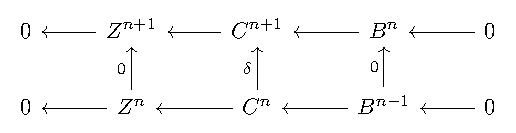
\includegraphics{lectures/0/pictures/cd_13}
    \end{center}

    Видно, что эта диаграмма~--- часть короткой точной последовательности комплексов. Она даёт нам длинную точную последовательность:
    \[ \ldots \leftarrow B^{n} \leftarrow Z^{n} \leftarrow H^n\lr*{C_{\bullet}, G} \leftarrow B^{n - 1} \leftarrow Z^{n - 1} \leftarrow \ldots \]
    Разбивая длинную точную последовательность на короткие точные последовательности мы получаем:
    \[ 0 \leftarrow \Ker\lr*{Z^n \to B^n} \xleftarrow{h} H^n\lr*{C_{\bullet}; G} \leftarrow \Coker\lr*{Z^{n - 1} \to B^{n - 1}} \leftarrow 0\]
    А теперь заметим, что  $\Ker\lr*{Z^n \to B^n} = \Hom\lr*{H_{n}(C_{\bullet}), G}$. Таким образом, мы получаем  расщепимую точную последовательность:
    \[ 0 \to \Coker\lr*{Z^{n - 1} \to B^{n - 1}}  \to H^n\lr*{C_{\bullet}; G} \to \Hom\lr*{H_{n}(C_{\bullet}), G} \to 0. \]
    
    \begin{definition}
        Пусть $H$~--- абелева группа. Тогда её \emph{свободная резольвента}~--- это точная последовательность
        \[ \ldots \to F_{2} \xrightarrow{f_2} F_{1} \xrightarrow{f_1} F_0 \xrightarrow{f_0} H \to 0, \]
        в которой каждая группа $F_n$ свободная.
    \end{definition}

    Применяя к этой точной последовательности функтор $\Hom(-, G)$  мы можем потерять точность, но во всяком случае, получим цепной комплекс:
    \[ \leftarrow F_2^* \xleftarrow{f_2^*} F_1^* \xleftarrow{f_1^*} F_0^* \xleftarrow{f_0^*} H^* \leftarrow 0\]

    Будем обозначать группы когомологий свободной резольвенты, как $H^n(F, G)$. Нам понадобится следующее утверждение из гомологической алгебры:

    \begin{lemma}\label{FreeResolventProp}
        Пусть даны свободные резольвенты $F$ и $F'$ абелевых групп $H$ и $H'$. Тогда любой гомоморфизм $\alpha\colon H \to H'$
        можно продолжить до цепного отображения $F \to F'$. Кроме того, любые два таких цепных отображения, продолжающие гомоморфизм $\alpha$, цепно гомотопны.

        Для любых двух свободных резольвент $F$ и $F'$ группы $H$ существуют канонические изоморфизмы
        \[ H^n(F; G) \cong H^n(F'; G). \]
    \end{lemma}

    У любой абелевой группы $H$ есть свободная резольвента вида
    \[ 0 \to F_1 \to F_0 \to H \to 0 \]
    с $F_i = 0$ при $i > 1$, которую мы сейчас построим.

    Выберем в $H$ набор образующих и пусть $F_0$~--- группа, свободно порожденная этими образующими.
    Тогда у нас есть сюръективный гомоморфизм $f_0\colon F_0 \to H$, переводящий элементы базиса в образующие $H$. Его ядро будет свободно, как
    подгруппа свободной группы, поэтому мы можем положить $F_1 = \Ker{f_0}$, а в качестве $f_1$ взять включение $\Ker{f_0} \hookrightarrow F_0$.

    Для этой свободной резольвенты мы имеем $H^n(F; G) = 0 \ \forall n > 1$, поэтому, из леммы~\ref{FreeResolventProp}  мы получаем, что это
    должно быть верно для всех свободных резольвент.

    Таким образом, единственная интересная группа из $H^n(F; G)$~--- это $H^1(F; G)$. Эта группа зависит лишь от $H$ и $G$, поэтому
    обычно её обозначают $\Ext(H, G)$\footnote{Вообще говоря, в гомологической алгебре функтор $\Ext$ обычно интерпретируют, как множество классов эквивалентности расширений $G$ посредством $H$, но в алгебраической топологии такая интерпретация редко нужна. }.

    Так вот, из построения свободной резольвенты для группы $H$ и определения когомологий мы теперь наконец можем заметить, что
    \[ \Coker\lr*{Z^{n - 1} \to B^{n - 1}} = \Ext\lr*{H_{n - 1}(C_{\bullet}), G}. \]

    Теперь мы наконец можем заключить, что мы доказали формулу универсальных коэффициентов для когомологий:

    \begin{theorem}[Об универсальных коээфициентах для когомологий]
        Пусть $C_{\bullet}$~--- цепной комплекс. Тогда его группы когомологий определяются расщепимыми короткими точными последовательностями
        \[ 0 \to \Ext\lr*{H_{n - 1}(C_{\bullet}), G} \to H^{n}(C; G) \to \Hom\lr*{H_{n}(C), G} \to 0 \]
    \end{theorem}

    Вообще говоря, это утверждение достаточно полезно, потому что на конечнопорожденных абелевых группах функтор $\Ext$ несложно посчитать:
    \begin{itemize}
        \item $\Ext\lr*{H \oplus H', G} \cong \Ext\lr*{H, G} \oplus \Ext\lr*{H', G}$.
        \item $\Ext\lr*{H, G} = 0$, если $H$~--- свободна.
        \item $\Ext(\Z/n\Z, G) \cong G/nG$.
        \item Если $H$ конечно порождена, то имеет место изоморфизм
         \[ \Ext(H, \Z) \cong \mathrm{Tor}\lr*{H}. \]
    \end{itemize}

    Кроме того, теорема об универсальных коэффициентов позволяет вычислять когомологии, зная только гомологии.
    \begin{corollary}
        Если группы гомологий $H_n(C)$ и $H_{n - 1}(C)$ комплекса $C$, состоящего из свободных абелевых групп, конечно порождены и $T_n \subset H_n$ и $T_{n - 1} \subset H_{n - 1}$~--- подгруппы кручения, то
        \[ H^{n}\lr*{C; \Z} \cong (H_{n - 1}(C)/T_n) \oplus T_{n - 1}.\]
    \end{corollary}

    Это следствие даёт нам обобщение и формализацию примера~\ref{TorsionCohomology}.

    Кроме того, из всего этого дела есть еще одно замечательное следствие:

    \begin{corollary}
        Если $f\colon C_{\bullet} \to C_{\bullet}'$ индуцирует изоморфизм всех групп гомологий $H_{k}(C_{\bullet}) \cong H_{k}\lr*{C_{\bullet}'}$.
        Тогда отображения $f^{*}\colon H^{k}\lr*{C_{\bullet}; G} \cong H^{k}\lr*{C_{\bullet}'; G}$.
    \end{corollary}
    \begin{proof}
        Действительно, достаточно заметить, что из свойств свободной резольвенты мы знаем, что отобрежение цепных комплексов индуцирует такую вот диаграмму:
        \begin{center}
            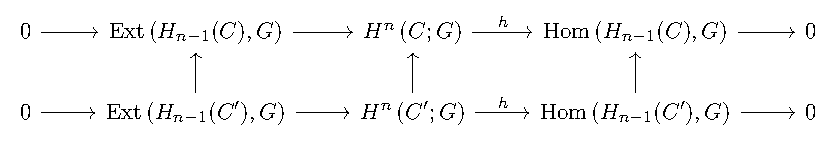
\includegraphics{lectures/0/pictures/cd_14}
        \end{center}
        Применяя 5-лемму и индукцию, мы получаем нужное.
    \end{proof}

    \subsection{Умножение в когомологиях}

    Пусть $R$~--- коммутативное и ассоциативное кольцо.

    Пусть $\varphi \in C^{k}\lr*{X; R}, \ \psi \in C^{\ell}\lr*{X; R}$. Тогда их произведением определяется таким образом:
    \[ \varphi \smile \psi \in C^{k + \ell}, \quad (\varphi \smile \psi)(\sigma) = \varphi(\sigma\vert_{[v_0 \ldots v_k]}) \cdot \psi(\sigma\vert_{[v_k \ldots v_{k + \ell}]}), \]
    где $\sigma\colon \Delta^{k + \ell} \to X$~--- сингулярный симплекс.

    \begin{lemma}
        Для кограницы $\smile$-произвения справедлива следующая формула:
        \[ \delta(\varphi \smile \psi) = \delta \varphi \smile \psi + (-1)^k \varphi \smile \delta \psi. \]
    \end{lemma}

    \begin{proof}
        Пусть $\sigma\colon \Delta^{k + \ell} \to X$~--- сингулярный симплекс. Тогда
        \[ (\delta \varphi \smile \psi)(\sigma) = \sum_{i = 0}^{k + 1} (-1)^{i} \varphi(\sigma\vert_{[v_0, \ldots, \hat{v_i}, \ldots, v_{k + 1}]}) \psi(\sigma\vert_{[v_{k + 1} \ldots v_{k + \ell + 1}]})\]
        Распишем теперь второй кусок:
        \[ (-1)^k (\varphi \smile \delta \psi) = \sum_{i = k}^{k + \ell + 1} (-1)^i \varphi(\sigma\vert_{[v_0 \ldots v_k]}) \psi(\sigma\vert_{[v_{k}, \ldots, \hat{v_i}, \ldots, v_{k + \ell + 1}]}) \]
        Когда мы сложим эти две суммы, последнее слагаемое первой суммы сократится с первым слагаемым второй, а всё, что останется~--- как раз $\delta(\varphi \smile \psi)(\sigma) = (\varphi \smile \psi)(\partial \sigma)$.
    \end{proof}
    
    \begin{remark}
       Таким образом, $\delta (\varphi \smile \psi) = \delta \varphi \smile \psi \pm \delta \psi \smile \varphi$. Из этого следует, что произведение коциклов~--- коцикл.
       Также это сразу даёт нам, что произведение коцикла и кограницы (в любом порядке)~--- кограница:
        \[ \varphi \smile \delta \psi = \pm \delta(\varphi \smile \psi)\]

        Это даёт нам ассоциативное дистрибутивное умножение
        \[ \smile \colon H^{k}\lr*{X; R} \times H^{\ell} \to H^{k + \ell} \lr*{X; R}. \]
        Таким образом, при помощи $\smile$-произведения, мы наделили \[ H^{*}\lr*{X; R} = \bigoplus_{n = 0}^{\infty} H^{n}\lr*{X; R} \] структурой кольца (а на самом деле, градуированной алгебры).

        Если в кольце $R$ есть единица, то единицей относительно $\smile$-произведения будет нольмерный коцикл $1 \in H^{0}\lr*{X; R}$, принимающий значение 1 на любом нульмерном сингулярном симплексе.
        
    \end{remark}
    
    \begin{remark}
       Это показывает нам отдельную пользу когомологий: например, у $\C \mathrm{P}^2$ и $S^4 \vee S^2$  все группы гомологий и группы когомлогий совпадают, а кольца когомологий отличаются.
    \end{remark}   
    









    \newpage
    \section{Комплексная алгебраическая геометрия}
    % Комплексные многообразия, касательное пространство, якобиан голоморфного отображения. Векторные расслоения, дифференциальные формы.
        \subsection{Комплексные многообразия}

    \begin{definition}
        \emph{Комплексным многообразием} $M$ называется гладкое многообразие, допускающее
        такое открытое покрытие $\{ U_{\alpha} \}_{\alpha \in I}$ и такие координатные отображения
        $\varphi_{\alpha}\colon U_{\alpha} \to \C^n$, что все функции перехода $\varphi_{\alpha} \circ \varphi_{\beta}^{-1}$
        голоморфны на $\varphi_{\beta}(U_{\alpha} \cap U_{\beta})$.

        Функция $f$ на открытом подмножестве $U \subset M$ называется \emph{голоморфной}, если $\forall \alpha \in I$
        функция $f \circ \varphi^{-1}_{\alpha}$ голоморфна в $\varphi_{\alpha}(U_{\alpha} \cap U)$.

        Набор $z = (z_1, \ldots, z_n)$ функций на $U \subset M$ называется \emph{голоморфной системой координат}, если $\varphi_{\alpha} \circ z^{-1}$ и $z \circ \varphi^{-1}_{\alpha}$ голоморфны на $z(U \cap U_{\alpha})$ и $\varphi_{\alpha}(U \cap U_{\alpha})$
        для всех $\alpha$.

        Отображение $f\colon M \to N$, где $M$ и $N$~--- комплексные многообразия, называется \emph{голоморфным}, если в голоморфных локальных координатах оно
        задаётся голоморфными функциями.
    \end{definition}

    \begin{example}[Примеры комплексных многообразий]
        Приведём какие-нибудь примеры комплексных многообразий:

        \begin{enumerate}
            \item Одномерное комплексное многообразие называют \bf{римановой поверхностью}.

            \item $P\mathbb{C}^n  = (\C^{n + 1}\setminus \{ 0 \})/\{ z \sim \lambda z \} = \mathbb{P}^n$~--- комплексное проективное пространство.
            Это пространство компактно, так как есть непрерывное сюръективное отображение $S^n \subset \C^{n + 1} \to \mathbb{P}^n$.

            \item Пусть $\Lambda = \Z^{k} \subset \mathbb{C}^n$~--- дискретная решётка. Факторгруппа $\C^n/\Lambda$ обладает структурой
            комплексного многообразия, которую индуцирует проекция $\pi\colon \C^n \to \C^n/\Lambda$.
            Это многообразие компактно тогда и только тогда, когда $k = 2n$ и в этом случае $\C^n / \Lambda$ называется \bf{комплексным тором}.

            \item \textcolor{magenta}{Тут был еще пример, что при неразветвлённом накрытии структура комплексного многообразия наследуется, но я хз, что такое разветвлённое накрытие.}
        \end{enumerate}
    \end{example}

    \noindent\bf{Касательное пространство к комплексному многообразию.}

        Пусть $M$~--- комплексное многообразие, $p \in M$, а $z = (z_{1}, \ldots, z_n)$~--- система голоморфных координат в окрестности $p$.
        В случае комплексного многообразия имеются три различных понятия \emph{касательного пространства} к $M$ в точке $p \in M$.

        \begin{enumerate}
            \item Рассмотрим $M$, как вещественное $2n$-многообразие. Тогда $T_{\R, p}M$~--- пространство
            $\R$-линейных дифференцирований кольца $C^{\infty}(M, \R)$ (с носителем в окрестности $p$).
            Если мы представим голоморфные координаты в виде $z_j = x_j + i y_j$, то $T_{\R, p}M$ будет иметь базис
            $\{ \frac{\partial }{\partial x_j}, \ \frac{\partial}{\partial y_j}\}$, как векторное пространство над $\R$.

            \item Пространство  $T_{\R, p}M$ можно комплексифицировать при помощи расширения скаляров, то есть рассмотреть
            \[ T_{\C, p}M \eqdef T_{\R, p}M \otimes_{\R} \C. \]
            $T_{\C, p}M$ называют \emph{комплексифицированным касательным пространством} к $M$ в точке $p$.
            Его можно реализовать, как пространство $\C$-линейных дифференцирований кольца $C^{\infty}(M, \C)$ (опять же, фукнции с носителем в окрестности $p$).
            Соотвественно, там можно выбрать базис $\{ \frac{\partial}{\partial x_j}, \frac{\partial}{\partial y_j}\}$, а при замене базиса на комлпексные обозначения
            \[ \frac{\partial}{\partial z_j} = \frac{1}{2} \lr*{\frac{\partial}{\partial x_j} - i \frac{\partial}{\partial y_j}}, \ \frac{\partial}{\partial\overline{z_j}} = \frac{1}{2}\lr*{\frac{\partial}{\partial x_j} + i \frac{\partial}{\partial y_j}}. \]
            <<более стандартный>> базис $\{ \frac{\partial}{\partial z_j}, \ \frac{\partial}{\partial \overline{z_j}}\}$.

            \item Подпространство $T'_{p}M = \Span\{ \frac{\partial }{\partial z_j} \} \le T_{\C, p}M$ называется  \emph{голоморфным касательным пространством} к $M$
            в точке $p$. Оно может быть реализовано, как подпространство в $T_{\C, p}M$, состоящее из дифференцирований, обращающихся в ноль на антиголоморфных функциях (таких $f$, что $\overline{f}$~--- голоморфна).
            Соответственно, подпространство $T''_{p}M = \Span \{ \frac{\partial }{\partial \overline{z_j}}\}$ называется \emph{антиголоморфным касательным пространством} к $M$ в точке $p$.
            Ясно, что
            \[ T_{\C, p}M = T'_{p}M \oplus T''_{p}M. \]
        \end{enumerate}

        Заметим, что для  комплексных многообразий $M, N$ любое $f \in C^{\infty}(M, N)$ индуцирует линейное отображение
        \[ f_{*}\colon T_{\R, p}M \to T_{\R, f(p)}N \]
        а значит и линейное отображение
        \[ f_{*}\colon T_{\C, p}M \to T_{\C, f(p)}N, \]
        но не отображение $T'_{p}M \to T'_{f'(p)}N$ для всех $p \in M$.

    На самом деле, отображение $f\colon M \to N$ голоморфно тогда и только тогда, когда
    \[ f_{*}(T'_{p}M) \subset T'_{f(p)}N \quad \forall p \in M. \]
    То есть, когда голоморфное касательное пространство отображается в голоморфное.

    Заметим, что также, поскольку $T_{\C, p}M = T_{\R, p}M \otimes \C$, операция сопряжения, переводящая
    \[ \frac{\partial}{\partial z_j} \mapsto \frac{\partial}{\partial \overline{z_j}} \]
    корректно определена на $T_{\C, p}M$ и, как нетрудно заметить, $T''_{p}M = \overline{T'_{p}M}$. Отсюда следует, что проекция
    \[ T_{\R, p}M \to T_{\C, p}M \to T'_{p}M \]
    есть $\R$-линейный изоморфизм.
    
    Это обстоятельство позволяет заниматься геометрией исключительно в голоморфном касательном пространстве.
    
    \begin{example}
        Пусть $z(t) \colon [0, 1] \to \C$~--- гладкая кривая.  Тогда $z(t) = x(t) + iy(t)$ и в качестве касательной мы можем взять
        \[ x'(t) \frac{\partial}{\partial x} + y'(t) \frac{\partial}{\partial y} \text{ в } T_{\R}\C \text{, либо } z'(t) \frac{\partial}{\partial z} \text{ в } T'\C. \]
    \end{example}


    \begin{definition}
        Пусть теперь $M, N$~--- комплексные многообразия, $z = (z_1, \ldots, z_n)$~--- голомрфные координаты в окрестности
    точки $p \in M$, а $(w_1, \ldots, w_n)$~--- голоморфные координаты в окрестности точки $q = f(p)$, где $f\colon M \to N$~--- голоморфное отображение.
    В связи с различными понятиями касательных пространств, мы имеем и различные понятия \emph{якобиана} $f$.

    \begin{enumerate}
        \item Пусть $z_j = x_j + i y_j, \ w_{k} = u_{k} + i v_{k}$. Тогда в базисах
        $\{ \frac{\partial}{\partial x_j}, \frac{\partial}{\partial y_j}\}$ и $\{ \frac{\partial}{\partial u_k}, \frac{\partial}{\partial v_k}\}$ пространств
        $T_{\R, p}M$ и $T_{\R, q}N$ линейное отображение $f_{*}$ задаётся $2m \times 2n$-матрицей
        \[ \cJ_{\R}(f) = \begin{pmatrix} \frac{\partial u_k}{\partial x_j} & \frac{\partial u_k}{\partial y_j} \\ \frac{\partial v_k}{\partial x_j} & \frac{\partial v_k}{\partial y_j} \end{pmatrix}. \]

        В базисах $\{ \frac{\partial}{\partial z_j}, \frac{\partial}{\partial \overline{z_j}}\}$ и $\{ \frac{\partial}{\partial w_j}, \frac{\partial}{\partial \overline{w_k}}\}$ пространств
        $T_{\C, p}M$ и $T_{\C, q}N$ отображение $f_{*}$ задаётся матрицей
        \[ \cJ_{\C}(f) = \begin{pmatrix} \cJ(f) & 0 \\ 0 & \overline{\cJ(f)} \end{pmatrix}, \text{ где } \cJ(f) = \lr*{ \frac{\partial w_k}{\partial z_j} }_{k, j}. \]
    \end{enumerate}

    \end{definition}

    \begin{remark}\label{rem1}
       В частности, отметим, что $\rank \cJ_{\R}(f) = 2 \rank \cJ(f)$ и в случае $m = n$
       \[ \det\cJ_{\R}(f) = \det \cJ(f) \det \overline{\cJ(f)} = \left\lvert \det{\cJ(f)}\right\rvert^2 \ge 0, \]
        то есть голоморфные отображения \bf{сохраняют ориентацию}.
    \end{remark}

    Мы будем считать, что пространство $\C^n$ естественно ориентированно $2n$-формой
    \[ \lr*{\frac{i}{2}}^n (\mathrm{d}z_{1} \wedge \mathrm{d}\overline{z_1}) \wedge (\mathrm{d}z_{2} \wedge \mathrm{d}\overline{z_2}) \wedge \ldots \wedge (\mathrm{d}z_n \wedge \mathrm{d}\overline{z_n}) = \mathrm{d}x_1 \wedge \mathrm{d}y_1 \wedge \ldots \wedge \mathrm{d}x_n \wedge \mathrm{d}y_n. \]

    Ясно, что если $\varphi_{\alpha}\colon U_{\alpha} \to \C^n$ и $\varphi_{\beta}\colon U_{\beta} \to \C^n$~--- голоморфные координатные отображения на
    комплексном многообразии $M$, то прообразы при $\varphi_{\alpha}$ и $\varphi_{\beta}$
    естественной ориентации на  $\C^n$ согласованы на $U_{\alpha} \cap U_{\beta}$.

    Соотвественно, любое комплексное многообразие \bf{имеет естественную ориентацию}, которая сохраняется
    при голоморфных отображениях.


    % Теорема об обратной функции, теорема о неявной функции, подмногообразия.
    \subsection{Когомологии де Рама и компактные когомологии}

	\begin{definition} 
		Комплекс $\Omega^{\bullet}(\R^n)$ вместе с оператором $\mathrm{d}$ называется \emph{комплексом де Рама} на $\R^n$.

		Соответственно, когомологии этого комлпекса называют \emph{когомологиями Де Рама} $\R^n$:
		\[
			H^{q}_{\mathrm{dR}}(\R^n) = \ker\lr*{\mathrm{d} \colon \Omega^{q}((\R^n)) \to \Omega^{q + 1}(\R^n)}/\mathrm{Im}\lr*{ \mathrm{d} \colon \Omega^{q - 1}(\R^n) \to \Omega^{q}(\R^n)}. 
		\]
	\end{definition}

	\begin{remark}
		То, что это комплекс, гарантируется тем, что $\mathrm{d}^2 = 0$ (и, соотвественно, в связи с этим мы имеем $\ker{\mathrm{d}} \supset \Im{\mathrm{d}}$).
	\end{remark}


	\begin{remark}
		Видно $\ker{\mathrm{d}}$~--- это замкнутые формы, а образ $\mathrm{d}$~--- точные формы. 	
		Например, $f(x, y) \mathrm{d}x + g(x, y) \mathrm{d}y$ замкнута тогда и только тогда, когда 
		\[
			\frac{\partial f}{\partial y} - \frac{\partial g}{\partial x} = 0.
		\]
	\end{remark}

	Класс когомологий формы $\omega$ мы будем обозначать $[\omega]$. 

	\begin{remark}
		Всё то же самое можно делать для открытого $U \subset \R^n$ таким образом: 
		\[
			\Omega^{\bullet}(U) = C^{\infty}(U) \otimes_{\R} \Omega^{\bullet}(\R^n).
		\]
		Таким образом, мы можем говорить о когомологиях де-Рама $H^{q}_{\dR}(U)$ для любого открытого подмножества $\R^n$. 
	\end{remark}

	Заметим, что гладкое отображение $f\colon U \to V$, где $U, V$~--- открытые  подмножества $\R^n$, индуцирует отображение на формах 
	\[
		f^{*}\colon \Omega^{q}(V) \to \Omega^{q}(U), \ \omega \mapsto f^{*}(\omega),
	\]
	а так как дифференциал коммутирует с пуллбеком (т.е. $\mathrm{d} f^{*}(\omega) = f^{*}(\mathrm{d}\omega)$, $f^{*}$ даст нам цепное отображение $\Omega^{\bullet}(V) \to \Omega^{\bullet}(U)$:


	\begin{center}
		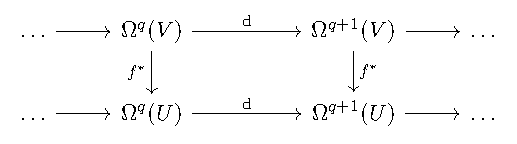
\includegraphics{lectures/7/pictures/cd_2.pdf}
	\end{center}

	\begin{definition} 
		\emph{Когомологии с компактным носителем} определяются следующим образом: рассмотрим комплекс дифференциальных форм с компактным носителем: 
		\[
			\Omega_{c}^{\bullet}(\R^n) \eqdef C^{\infty}_{0}(\R^n) \otimes_{\R} \Omega^{\bullet}(\R^n).
		\]
		Тогда когомологии с компактным носителем~--- это когомологии этого комплекса, мы будем обозначать их  $H^{q}_{c}(\R^n)$. 
	\end{definition}

	\begin{remark}
		Тут всё также корректно, так как $\mathrm{d}^2 = 0$. Но тут есть свои тонкости: нужно поступать аккуратнее с пуллбэком, так как пуллбэк формы с компактным носителем не обязан иметь компактный носитель. С другой стороны, если мы рассматриваем пулл-бэк при собственном отображении (т.е. таком, что прообраз компакта -- компакт), то всё выживает.  
	\end{remark}

	\begin{example}
		Вычислим $H^{\bullet}_{\dR}(\R)$.

		\begin{center}
			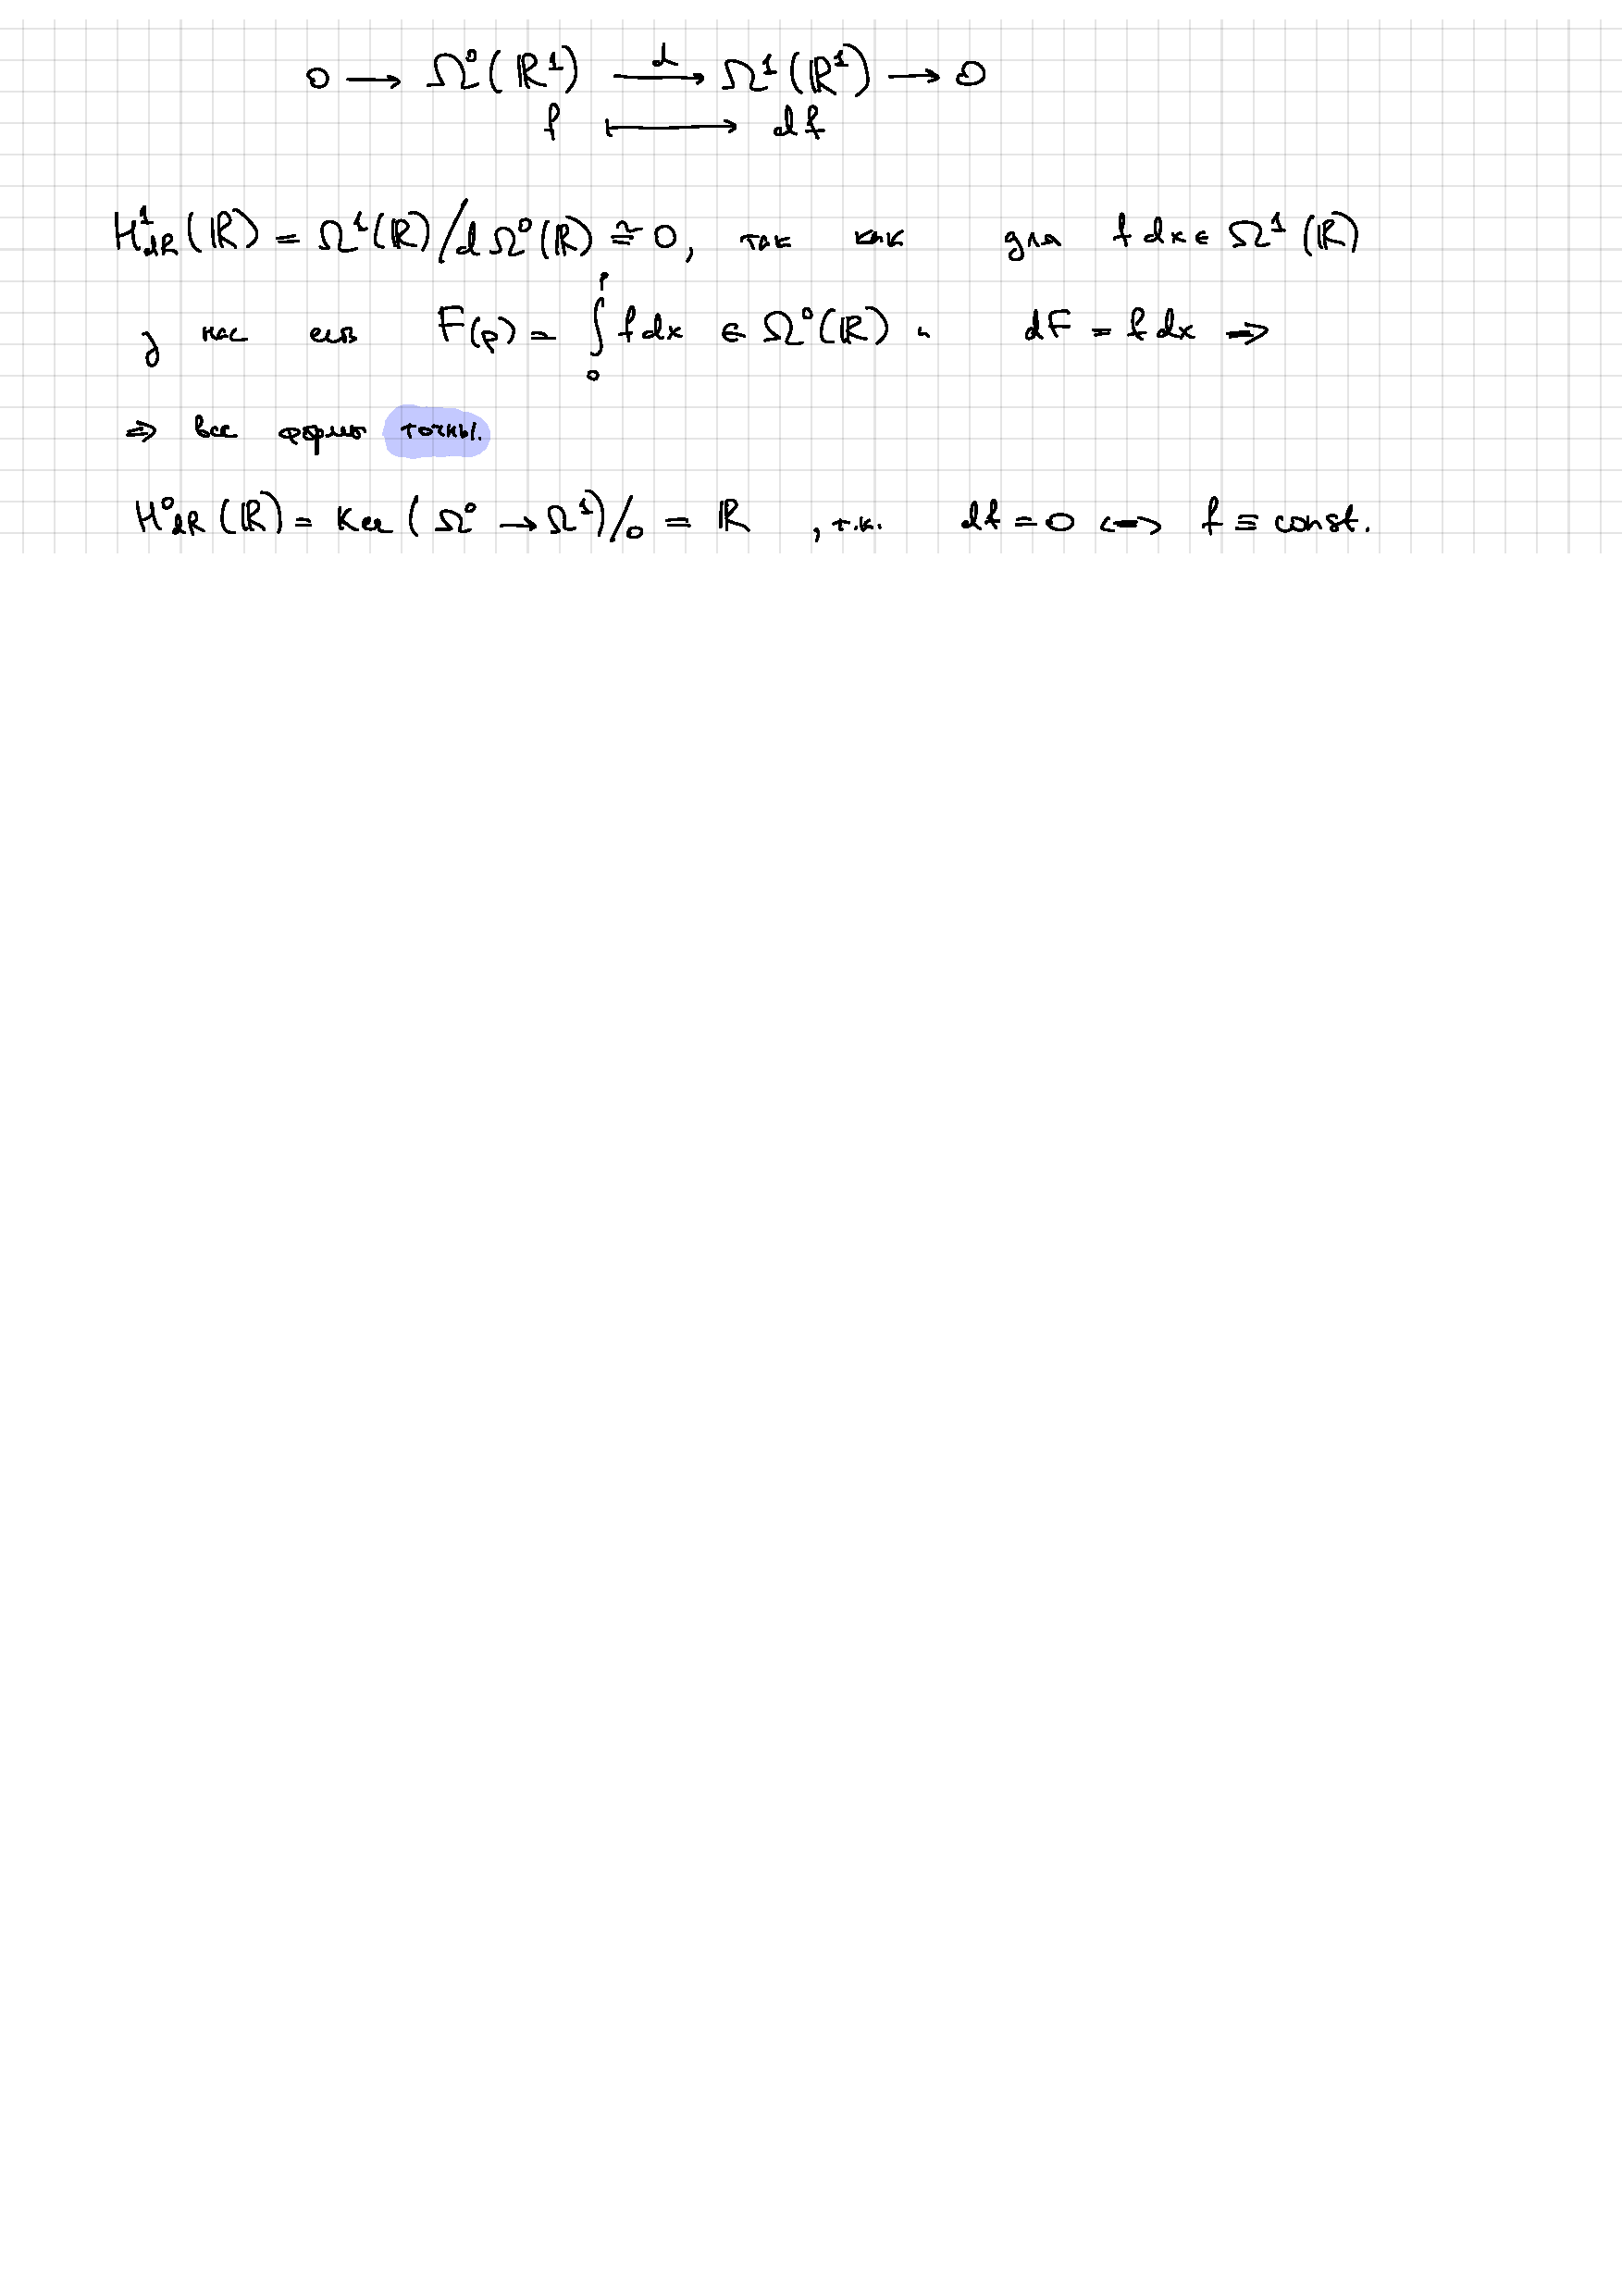
\includegraphics[scale = 0.6]{lectures/7/pictures/line_de_Rham.pdf}
		\end{center}

		Теперь вычислим компактные когомологии $H^{\bullet}_{c}(\R)$:
		\begin{center}
			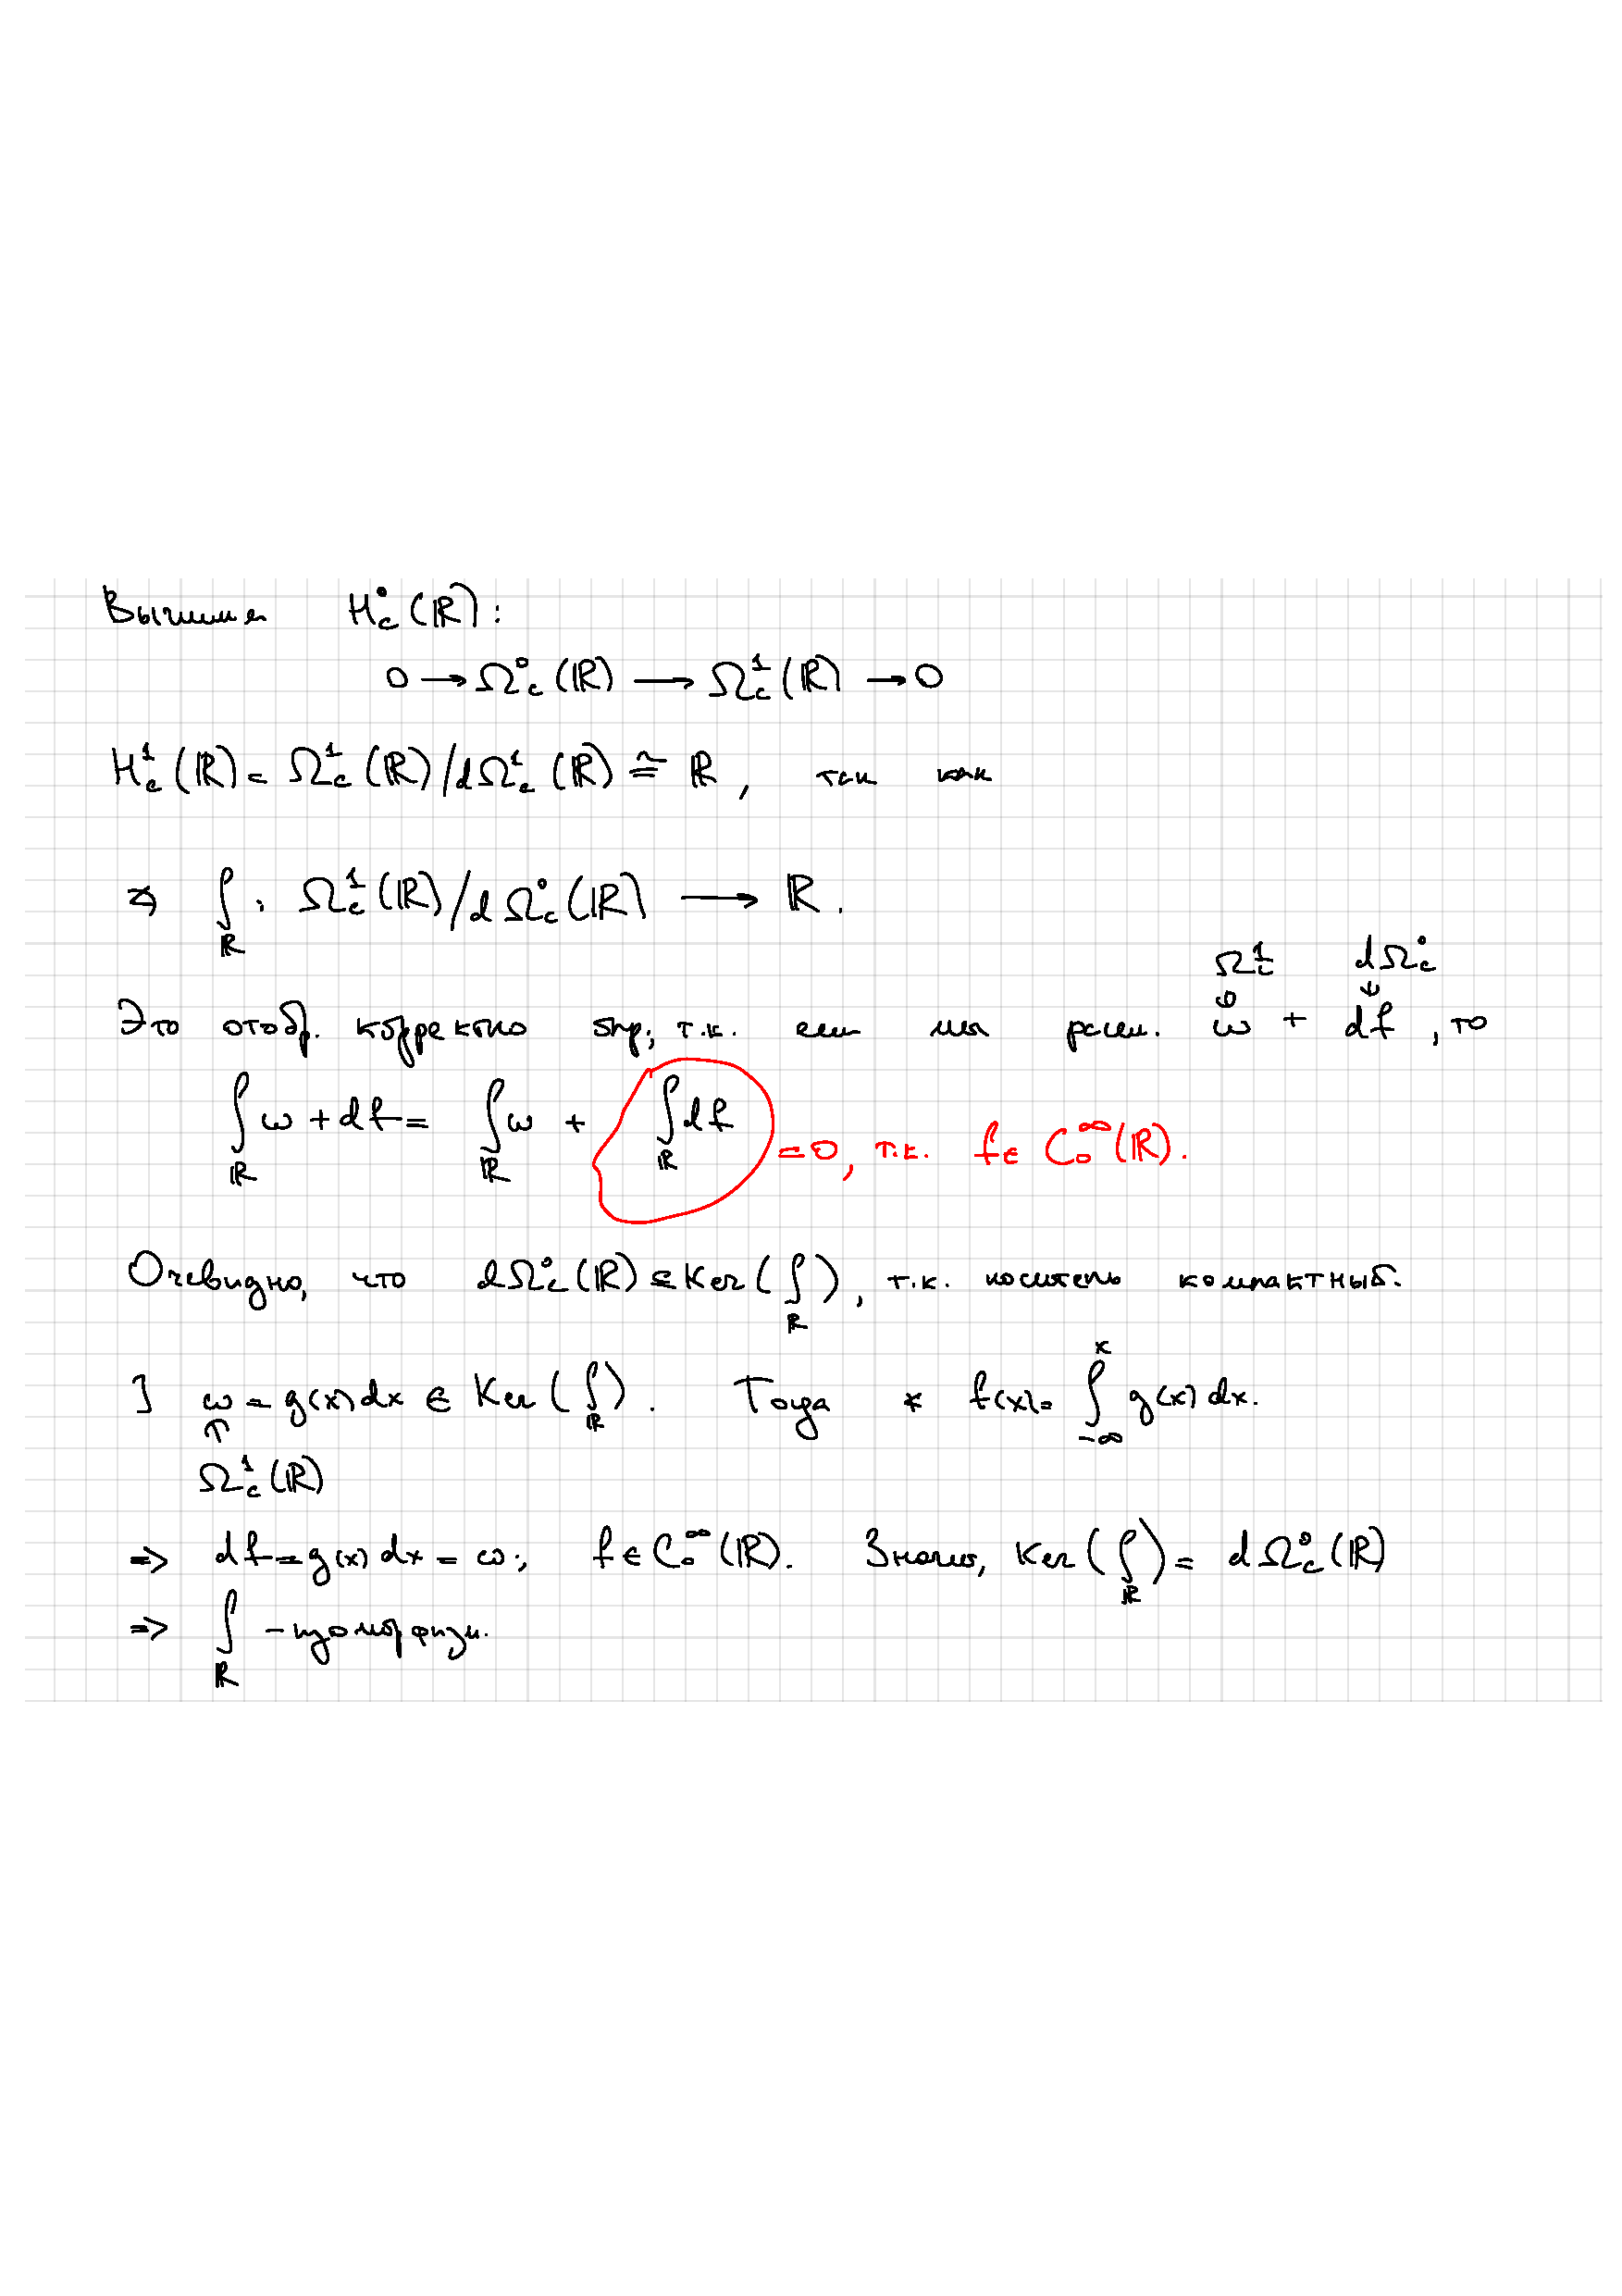
\includegraphics[scale = 0.6]{lectures/7/pictures/line_de_Rham_2.pdf}
		\end{center}

	\end{example}

	\subsection{Дифференциальные формы на многообразиях}

	На самом деле, тот факт, что гладкое отображение $f\colon U \to V$ индуцирует морфизм $f^* \colon \Omega^{\bullet}(V) \to \Omega^{\bullet}(U)$ (т.е., что дифференциал коммутирует с пуллбэком) на более изысканном языке означает, что $\Omega^*$ является контравариантным функтором из категории евклидовых пространств (и гладких отображений между ними) в категорию коммутативных дифференциальных градуированных алгебр. Коммутативность тут имеется в виду кососимметричная, то есть
	\[
		\tau \wedge \omega = (-1)^{\deg{\tau} \cdot \deg{\omega}} \omega \wedge \tau
	\]

	Более того, единственный такой функтор, совпадающий в нулевом члене с $C^{\infty}(\R^n)$~---  это как раз $\Omega^{\bullet}$.

	Действительно, из-за того, что $\Omega^{0}(\R^n) = C^{\infty}(\R^n)$, у нас сразу фиксирован базис из нужных $\mathrm{d}x_i$ (после того, как мы выбрали координатыне функции $x_i$), а дальше по линейности мы получаем всё те же 1-формы (и дальше по индукции). 
 

 	Этот функтор однозначно продолжается на категорию гладких многообразий. 

 	\begin{definition} 
 		Пусть $M$~--- гладкое многообразие, покрытое картами $\{ (U_{\alpha}, \varphi_{\alpha}) \}_{\alpha}$. Тогда дифференциальная форма $\omega$ на $M$ задаётся набором форм $\omega_{\alpha}$, каждая из которых задана в карте $U_{\alpha} \cong \R^n$, причём они согласованы на пересечении. 

 		Формальнее, у нас есть отображения 
 		\begin{center}
 			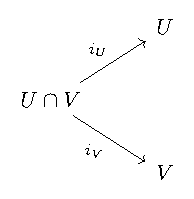
\includegraphics{lectures/7/pictures/cd_3.pdf}
 		\end{center}
 		и мы требуем, чтоб $i^*_{U} \omega_U = i^*_V \omega_V$ на $U \cap V$. 
 	\end{definition}

 	\begin{example}
 		Приведём несколько примером дифференциальных форм на многообразиях: 


 	\end{example}

 	\subsection{Точная последовательность Майера-Виеториса}

 	Начнём с напоминания про пуллбэк: если $f\colon M \to N$, причем в $M$ координаты $x_1, \ldots, x_m$,  а в $N$ координаты $y_1, \ldots, y_n$, то 
 	\[
 		f^{*}(\mathrm{d}y_i) = \sum_{j = 1}^n \frac{\partial y_i}{\partial x_j} \mathrm{d}x_j.
 	\] 

 	Тогда мы сможем считать и пуллбэки форм: 
 	\[
 		f^{*}(F(y_1, \ldots, y_n) \mathrm{d}y_1 \wedge \ldots \wedge \mathrm{d}y_k) = F(y_1(x_1, \ldots, x_m), \ldots) f^{*}(\mathrm{d}y_1) \wedge \ldots \wedge f^{*}(\mathrm{d}y_k).
 	\]

 	Но можно говорить и иначе (мы немного говорили про этот подход в первом параграфе). А именно, как мы помним, формы $\mathrm{d}y_i$ можно вычислять на касательных векоторах $\sum a_j \frac{\partial}{\partial y_j}$, как 
 	\[
 		\mathrm{d} y_i \lr*{\sum a_j \frac{\partial}{\partial y_j}} = a_i. 
 	\]
 	Тогда $k$-формы у нас действуют на наборах из $k$ векторов (как элемент $\Lambda^k T^*M$).

 	Пусть $f_* = \mathrm{d}f\colon TM \to TN$, тогда 
 	\[
 	 	f_*\lr*{\frac{\partial}{\partial x_j}} = \lr*{ \frac{\partial y_1}{\partial x_j}, \ldots, \frac{\partial y_n}{\partial x_j} }. 
 	 \] 
 	 Соответственно, пуллбэк  $f^*(\omega)$ мы тогда можем определить, как $k$-форму, действующую на наборах из $k$ векторов следующим образом: 
 	 \[
 	 	f^*(\omega)(v_1, \ldots, v_k) \eqdef \omega(f_*v_1, \ldots, f_* v_k). 
 	 \]
 	 Проверим, что для 1-форм это определение совпадает с предыдущим: 
 	 \[
 	 	f^*(\mathrm{d}y_i) = \sum a_j \mathrm{d}x_j, \quad a_j = \mathrm{d}y_i\lr*{f_* \frac{\partial}{\partial x_j}} = \mathrm{d}y_i\lr*{ \frac{\partial y_1}{\partial x_j}, \ldots, \frac{\partial y_n}{\partial x_j} } = \frac{\partial y_i}{\partial x_j},
 	 \]
 	  а этот коэффициент совпадает с тем, который был в предыдущем определении. Отсюда сразу следует, что это определение совпадает предыдущим и для  $k$-форм. 

 	  \begin{remark} 
 	  	Как мы уже отмечали, для форм с компактным носителем пулбэк определён только для собственных отображений. Зато определён \emph{пушфорвадр} (т.е. отображение в другую сторону) для открытых вложений (и, соответственно, пуллбэк для обратных отображений). Отсюда следует, в частности, что мы можем корректно (и так же как в обычном случае) определять формы с компактным носителем для многообразий. 
 	  \end{remark}

 	  Перейдём к \bf{точной последовательности Майера-Виеториса:}\\

 	  Пусть $M = U \cup V$, $U$  и $V$~--- открытые. Тогда у нас есть диаграммы: 

 	  \begin{center}
 	  	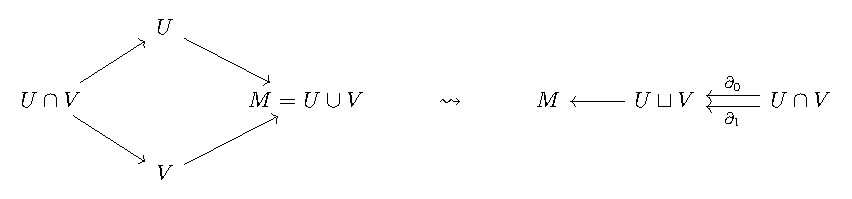
\includegraphics{lectures/7/pictures/cd_4.pdf}
 	  \end{center}

 	  Применяя функтор $\Omega^{\bullet}$, имеем 
 	  \begin{center}
 	  	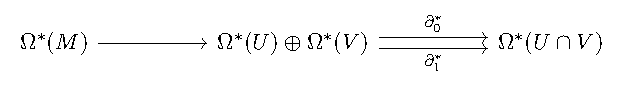
\includegraphics{lectures/7/pictures/cd_5.pdf}
 	  \end{center}

 	  \emph{Последовательностью Майера-Вьеториса} называется последовательность комплексов 
 	  \begin{center}
 	  		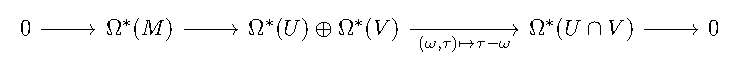
\includegraphics{lectures/7/pictures/cd_6.pdf}
 	  \end{center}

 	  \begin{remark}
 	  	Стрелка $\Omega^*(M) \to \Omega^*(U) \oplus \Omega^*(V)$~--- это сужение: $\omega \mapsto \omega\vert_U \oplus \omega\vert_{V}$. И, в следующей стрелке, когда мы берём разность, её мы тоже сужаем на $U \cap V$. 

 	  	Отметим, что под сужением на подмногообразие мы понимаем пулбек индуцированный вложением. 
 	  \end{remark}

 	  \begin{lemma} 
 	  	Последовательность Майера-Виеториса точна. 
 	  \end{lemma}
 	  \begin{proof}
 	  	Точность в первых двух членах очевидна (дольше писать, чем думать): 

 	  	 Проверим, что стрелка $\Omega^*(M) \to \Omega^*(U) \oplus \Omega^*(V)$ инъективна. Действительно, если $\omega\vert_{U} = 0$ и $\omega\vert_{V} = 0$, то $\omega = 0$ (так как $M = U \cup V$). 

 	  	 Теперь проверим точность в среднем члене. $\Ker\lr*{\Omega^*(U) \oplus \Omega^*(V) \to \Omega^*(U \cap V)} $~--- это формы $\tau \in \Omega^*(V)$ и $\omega \in \Omega^*(U)$, которые совпадают на $U \cap V$. Тогда просто по определению, так как формы согласованы на пересечении, из них можно склеить одну на $M$ (это доказывает включение $\Ker\lr*{\Omega^*(U) \oplus \Omega^*(V) \to \Omega^*(U \cap V)}  \subset \Im\lr*{ \Omega^*(M)  \to \Omega^*(U) \oplus \Omega^*(V)}$). С другой же стороны, если мы возьмём $\omega \in \Omega^*(M)$ и пройдём по двум стрелкам подряд, мы получим ноль: 
 	  	 \[
 	  	 	\omega \mapsto (\omega\vert_U, \omega\vert_V) \mapsto \lr*{\omega\vert_U - \omega\vert_V}\vert_{U \cap V} = \omega\vert_{U \cap V} - \omega\vert_{U \cap V} = 0. 
 	  	 \]
 	  	 Так мы получаем, что $\Im\lr*{ \Omega^*(M)  \to \Omega^*(U) \oplus \Omega^*(V)} \subset \Ker\lr*{\Omega^*(U) \oplus \Omega^*(V) \to \Omega^*(U \cap V)}$. 

 	  	 Теперь докажем точность в правом члене. Для этого воспользуемся разбиением единицы. 

 	  	 Докажем сначала для функций (для форм отсюда будет следовать афтоматически). Пусть $f \in \Omega^0(U \cap V)$, представим её в виде разности функций из $\Omega^0(U)$ и $\Omega^0(V)$. Пусть $\{ \rho_U, \rho_V \}$~--- разбиение единицы, подчиненное покрытию $\{ U, V \}$. Тогда мы определим $f_U = f \cdot \rho_V$, $f_V = - f \cdot \rho_U$. Тогда 
 	  	 \[
 	  	 	f \rho_V - (-f \rho_U) = f \cdot (\rho_U + \rho _V) = f \text{ на } U \cap V. 
 	  	 \]

 	  	 
 	  \end{proof}

 	  Теперь вспомним, что короткая точная последовательность комплексов индуцирует длинную точную последовательность когомологий. 

 	  \begin{center}
 	  		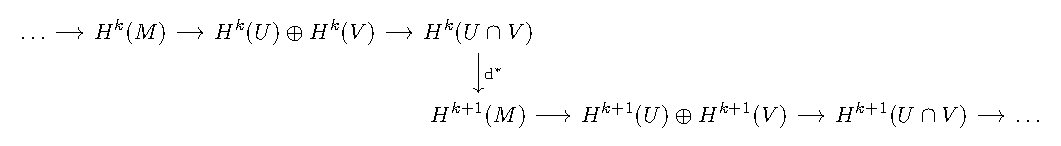
\includegraphics{lectures/7/pictures/cd_8.pdf}
 	  \end{center}

 	  Её также называют \bf{точной последовательностью Майера-Виеториса}. 

 	  Опишем явно, как выглядит связывающий кограничный гомоморфизм). Для этого нужно выполнить несложный диаграммный поиск. А именно, возьмём класс когомологий $[\omega] \in H^k(U \cap V)$ и выберем какого-то представителя $\omega \in \Omega^k(U \cap V)$. Отправим его наверх; так как это класс когомологий, $\mathrm{d}\omega = 0$. Теперь посмотрим из кого он пришёл и снова перейдём вверх. Так мы получим, что из пара форм $(\mathrm{d}(\rho_V \omega), - \mathrm{d}\rho_U \omega))$ согласована на пересечении и приходит из некоторой формы, которая и является $\mathrm{d}^*\omega$. 

 	  \begin{center}
 	  	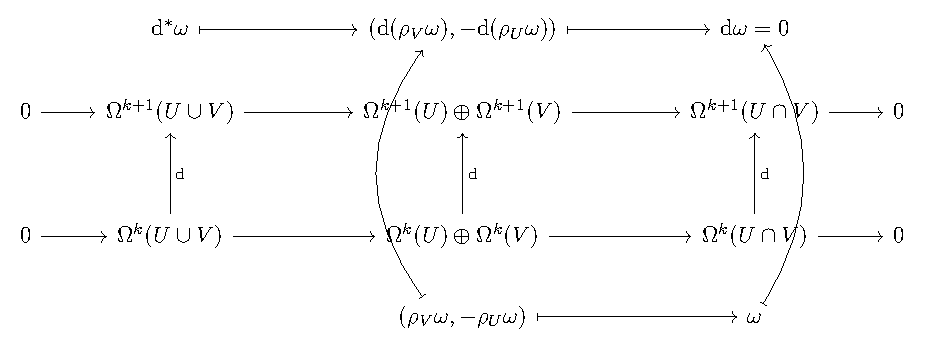
\includegraphics{lectures/7/pictures/cd_7.pdf}
 	  \end{center}

 	  Более того, слово <<некоторый>> тут исключительно в художественных целях, на самом то деле, как легко видеть из диаграммного поиска: 

 	  \[
 	  	\mathrm{d}^*[\omega] = \begin{cases} [-\mathrm{d}(\rho_V \omega)] \text{ на } U \\ [\mathrm{d}(\rho_U \omega)], \text{ на } V \end{cases}. 
 	  \]

	\noindent\bf{Последовательность Майера-Виеториса для форм с компактным носителем:}

	Напомним, что функтор $\Omega^{\bullet}_{c}(\_)$ удовлетворяет таким свойствам: 

	\begin{itemize}
		\item $\Omega^{\bullet}_{c}(\_)$ является контравариантным функтором относительно \emph{собственных отображений}. 

		\item $\Omega^{\bullet}_{c}(\_)$ является ковариантным функтором относительно \emph{открытых вложений}. 
	\end{itemize}


	В дальнейшем мы будем использовать именно ковариантную версию этого функтора. Тогда диаграмма 
	\begin{center}
		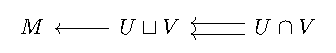
\includegraphics{lectures/7/pictures/cd_9.pdf}
	\end{center}
	индуцирует короткую точную последовательность комплексов 

	\begin{center}
		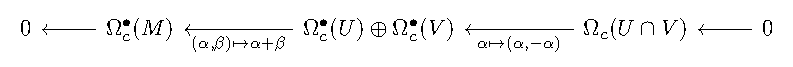
\includegraphics{lectures/7/pictures/cd_10.pdf}
	\end{center}

	\begin{lemma} 
		Последовательность Майера-Виеториса для форм с компактным носителем точна. 
	\end{lemma}
	\begin{proof}
		Здесь всё гораздо проще, чем в предыдущий раз. Обсудим точность в последнем члене. Гомоморфизм $\Omega^{\bullet}_{c}(M) \leftarrow \Omega_{c}^{\bullet}(U) \oplus \Omega_{c}^{\bullet}(V)$ сюръективен, так как прообразом формы $\omega$ является пара $(\rho_U \omega, \rho_V \omega)$ (где $\{ \rho_U, \rho_V \}$~--- разбиение единицы, подчинённое покрытию $\{ U, V \}$). 
	\end{proof}

	\begin{remark}
		Отметим, что в случае последовательности Майера-Виеториса для всех форм из формы на многообразии форму на кусочках мы получали так: 
		\[
			\omega \mapsto (\rho_V \omega, - \rho_U \omega).
		\]
		В то же время, в компактном случае мы поступаем несколько иначе 
		\[
			(\omega \rho_U, \omega\rho_V) \mapsto \omega. 
		\]
	\end{remark}
 	  
 	Тогда короткая точная последовательность комплексов индуцирует длинную точную последовательность когомологий (но, в другую сторону!)
 	\begin{center}
 		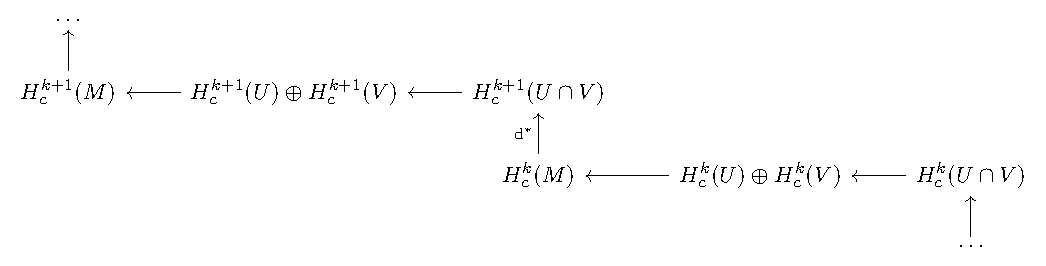
\includegraphics{lectures/7/pictures/cd_11.pdf}
 	\end{center}

 	\begin{example}
 		Переписать из книжки пример про окружность. 
 	\end{example}

 	
 	









    % Когомологии де Рама и Дольбо. 
       \subsection{Когомологии де Рама и Дольбо}

    Пусть $M$~--- гладкое многообразие. Обозначим за $A^{p}(M; \R)$
    пространство дифференциальных форм степени $p$ на $M$, а через $Z^{p}(M; \R)$
    подпространство замкнутых $p$-форм.

    Так как $d^2 = 0$, у нас есть (ко)цепной комплекс
    \[ A^{0}(M; \R) \to \ldots \to A^{p}(M; \R) \to A^{p + 1}(M; \R) \to \ldots \]
    а его группы когомологий называются группами \emph{когомологий де Рама} многообразия $M$.

    Иными словами, группы когомологий де Рама~--- это факторгруппы замкнутых форм по модулю точных
    \[ H_{\textrm{DR}}^{p}(M; \R)  = Z^{p}(M; \R) / d A^{p - 1}(M). \]

    Совершенно также мы можем рассматривать комплекснозначные формы и давать все соотвествующие определения (используя обозначения $ A^{p}(M)$ и аналогичные, то
    есть без коэффициентов):
    \[ H_{\mathrm{DR}}^{p}(M) = Z^{p}(M)/d A^{p - 1}(M) \]

    \begin{remark}
       Нетрудно заметить, что как и всегда с коэффициентами,
        \[ H^{p}_{\mathrm{DR}}(M) = H_{\mathrm{DR}}^{p}(M; \R) \otimes \C. \]
    \end{remark}

    Как мы заметили в самом первом параграфе, комплексифицированное кокасательное пространство раскладывается в голоморфную и антиголоморфную часть:
    \[ T^{*}_{\C, z}M = T_{z}^{*'} M \oplus T_{z}^{*''} M,  \]
    что дает нам разложение
    \[ \Lambda^n T^{*}_{\C, z}M = \bigoplus_{p + q = n}\lr*{ \Lambda^{p} T^{*'}_{z}(M) \otimes \Lambda^{q} T_{z}^{*''}(M)}, \]
    а это (по определению внешних форм) даёт нам
    \[ A^{n}(M) = \bigoplus_{p + q = n} A^{p, q}(M), \text{где }\]
    \[ A^{p, q}(M) = \{ \varphi \in A^{n}(M) \ \vert \ \varphi(z) \in \Lambda^{p}T_{z}^{*'}(M) \otimes \Lambda^q T_{z}^{*''}(M) \ \forall z \in M \}. \]

    Соотвественно, форму $\varphi \in A^{p, q}$ называют формой типа $(p, q)$. Обозначим за $\pi^{(p, q)}$ проекцию
    \[ A^{*}(M) \to A^{p, q}(M), \]
    так что для $\varphi \in A^{*}(M)$ имеем $\varphi = \sum \pi^{(p, q)}\varphi$.

    Если $\varphi A^{p, q}(M)$, то для любого $z \in M$
    \[ \mathrm{d}\varphi(z) \in \lr*{\Lambda^{p} T_{z}^{*'}M \otimes \Lambda^{q} T^{*''}_{z}M} \wedge T^{*}_{\C, z}M, \]
    \[ \mathrm{d}\varphi \in A^{p + 1, q}(M) \oplus A^{p, q + 1}(M). \]
    Определоим теперь для этих замечательных дифференциальных форма операторы
    \[ \overline{\partial}\colon A^{p, q}(M) \to A^{p, q + 1}, \quad \partial \colon A^{p, q}(M) \to A^{p + 1, q}(M) \]
    \[ \overline{\partial} = \pi^{(p, q + 1)} \circ \mathrm{d}, \quad \partial = \pi^{(p + 1, q)} \circ \mathrm{d}, \text{ то есть } d = \partial + \overline{\partial}. \]

    В локальных координатах $z = (z_{1}, \ldots, z_{n})$ форма $\varphi \in A^{n}(M)$ имеет тип  $(p, q)$, если она имеет
    представление в виде
    \[ \varphi(z) = \sum_{I, J} \varphi_{I, J}(z) \mathrm{d}z_{I} \wedge \mathrm{d}\overline{z}_{J} \]

    \begin{remark}
       Короче говоря, вся эта страшная белиберда была, чтоб сказать, что бывают не только голоморфные дифференциальные формы, но и такие, где
        один кусок голоморфный, а другой антиголоморфный.
    \end{remark}

   Дифференцировать эти формы можно вполне естественным образом:
    \[ \overline{\partial}\varphi(z) = \sum_{I, J, j} \frac{\partial}{\partial \overline{z_{j}}} \varphi_{I J}(z) \mathrm{d}\overline{z}_{j} \wedge \mathrm{d}z_{I} \wedge \mathrm{d}\overline{z}_{J}, \quad \partial \varphi(z) = \sum_{I, J, i} \frac{\partial \varphi}{\partial z_i} \varphi_{I J}(z) \mathrm{d}z_{i} \wedge \mathrm{d}z_{I} \wedge \mathrm{d}\overline{z}_{J}.  \]

    В частности, форма типа $(q, 0)$ называется \emph{голоморфной}, если $\overline{\partial}\varphi = 0$. Ясно, что это имеет место тогда и только тогда, когда 
    \[
       \varphi(z) = \sum_{I\colon |I| = q} \varphi_{I}(z) \mathrm{d}z_{I}, \text{ где }
    \]
    функции $\varphi_{I}(z)$ голоморфны. 

    Отметим, что поскольку разложение $T^{*}_{\C, z} = T^{*'}_{z} \oplus T_{z}^{*''}$ сохраняется при голоморфных отображениях, тоже самое будет верно и для $A^{\bullet} = \bigoplus_{(p, q)} A^{(p, q)}$. Действительно, если $f\colon M \to N$~--- голоморфное отображение комплексных многообразий, то $f^{*}\lr*{A^{p, q}(N)} \subset A^{p, q}(M)$ и $\overline{\partial} \circ f^{*} = f^{*} \circ \overline{\partial}$.

    Пусть $Z^{p, q}_{\overline{\partial}}(M)$~--- пространство $\partial$-замкнутых форм типа $(p, q)$. Тогда, так как
    \[
       \frac{\partial^2}{\partial\overline{z_i}\partial\overline{z_j}} = \frac{\partial^2}{\partial\overline{z_j}\partial\overline{z_i}}
    \]
    мы будем иметь $\overline{\partial}^2 = 0$ на $A^{(p, q)}$, откуда мы получим 
    \[
        \overline{\partial}\lr*{A^{p, q}(M)} \subset Z^{p, q + 1}_{\overline{\partial}}(M),
     \] 
     что позволяет определить \emph{группы когомологий Дольбо} как 
     \[
        H^{p, q}_{\overline{\partial}}(M) = Z^{p, q}_{\overline{\partial}}(M)/\overline{\partial}\lr*{A^{p, q - 1}(M)}
     \]

     \begin{theorem}[$\overline{\partial}$-лемма Пуанкаре] 
        Для полидиска $\Delta = \Delta(r) \subset \C^n$ имеет место равенство 
        \[
           H_{\overline{\partial}}^{p, q}(\Delta) = 0, q \ge 1.
        \]
     \end{theorem}
     \begin{proof}
        \textcolor{Emerald}{Какое-то очень уж неприятное. Лучше сначала узнать, как обычная лемма Пуанкаре про то, что в односвзяной области замкнутая форма точна, доказыватся.}
     \end{proof}

     \subsection{Пучки и когомологии}

     \begin{definition} 
        Пусть $X$~--- топологическое пространство. \emph{Пучок $\cF$} на $X$ сопоставляет каждому открытому множеству $U \subset X$ группу (или кольцо) $\cF(U)$ (которое мы будем называть группой \emph{сечений} $\cF$ над $U$) и каждой паре $U \subset V$ открытых подмножеств $X$ гомоморфизм $r_{VU}\colon \cF(V) \to \cF(U)$\footnote{тут буква $r$ от слова \emph{restriction}.}, называемый \emph{гомоморфизмом ограничения}, причём так, что

        \begin{enumerate}
           \item Для любой тройки $U \subset V \subset W$ открытых множеств выполняется
           \[
              r_{WU} = r_{WV} \circ r_{VU}.
           \]
           В силу этого соотношения по аналогии с ограничениями функций принято писать $r_{WU}(\sigma) = \sigma\vert_{U}$ (в общем $r_{WU}$~--- гомомрфизм сужения с $V$ на $U$).

           \item $r_{UU} = \id, \ \cF(\varnothing) = 0$.

           \item Для любой пары открытых множеств $U, V \subset M$ и сечений $\sigma \in \cF(U)$, $\tau \in \cF(V)$, таких что $\sigma\vert_{U \cap V} = \tau\vert_{U \cap V}$ найдётся такое сечение $\rho \in \cF(U \cup V)$, что 
           \[
              \rho\vert_{U} = \sigma, \quad \rho\vert_{V} = \tau.
           \]
           \item Если $\sigma \in \cF(U \cup V)$ и $\sigma\vert_{U} = \sigma\vert_{V} = 0$, то $\sigma = 0$.
        \end{enumerate}
     \end{definition}

     \noindent\bf{Очень хорошие пучки, которые мы будем часто встречать:}

     \begin{enumerate}
        \item 
     \end{enumerate}


    




\end{document}
